\documentclass[twoside]{book}

% Packages required by doxygen
\usepackage{fixltx2e}
\usepackage{calc}
\usepackage{doxygen}
\usepackage[export]{adjustbox} % also loads graphicx
\usepackage{graphicx}
\usepackage[utf8]{inputenc}
\usepackage{makeidx}
\usepackage{multicol}
\usepackage{multirow}
\PassOptionsToPackage{warn}{textcomp}
\usepackage{textcomp}
\usepackage[nointegrals]{wasysym}
\usepackage[table]{xcolor}

% Font selection
\usepackage[T1]{fontenc}
\usepackage[scaled=.90]{helvet}
\usepackage{courier}
\usepackage{amssymb}
\usepackage{sectsty}
\renewcommand{\familydefault}{\sfdefault}
\allsectionsfont{%
  \fontseries{bc}\selectfont%
  \color{darkgray}%
}
\renewcommand{\DoxyLabelFont}{%
  \fontseries{bc}\selectfont%
  \color{darkgray}%
}
\newcommand{\+}{\discretionary{\mbox{\scriptsize$\hookleftarrow$}}{}{}}

% Page & text layout
\usepackage{geometry}
\geometry{%
  a4paper,%
  top=2.5cm,%
  bottom=2.5cm,%
  left=2.5cm,%
  right=2.5cm%
}
\tolerance=750
\hfuzz=15pt
\hbadness=750
\setlength{\emergencystretch}{15pt}
\setlength{\parindent}{0cm}
\setlength{\parskip}{0.2cm}
\makeatletter
\renewcommand{\paragraph}{%
  \@startsection{paragraph}{4}{0ex}{-1.0ex}{1.0ex}{%
    \normalfont\normalsize\bfseries\SS@parafont%
  }%
}
\renewcommand{\subparagraph}{%
  \@startsection{subparagraph}{5}{0ex}{-1.0ex}{1.0ex}{%
    \normalfont\normalsize\bfseries\SS@subparafont%
  }%
}
\makeatother

% Headers & footers
\usepackage{fancyhdr}
\pagestyle{fancyplain}
\fancyhead[LE]{\fancyplain{}{\bfseries\thepage}}
\fancyhead[CE]{\fancyplain{}{}}
\fancyhead[RE]{\fancyplain{}{\bfseries\leftmark}}
\fancyhead[LO]{\fancyplain{}{\bfseries\rightmark}}
\fancyhead[CO]{\fancyplain{}{}}
\fancyhead[RO]{\fancyplain{}{\bfseries\thepage}}
\fancyfoot[LE]{\fancyplain{}{}}
\fancyfoot[CE]{\fancyplain{}{}}
\fancyfoot[RE]{\fancyplain{}{\bfseries\scriptsize Generated on Sun Aug 16 2015 15\+:14\+:16 for My Project by Doxygen }}
\fancyfoot[LO]{\fancyplain{}{\bfseries\scriptsize Generated on Sun Aug 16 2015 15\+:14\+:16 for My Project by Doxygen }}
\fancyfoot[CO]{\fancyplain{}{}}
\fancyfoot[RO]{\fancyplain{}{}}
\renewcommand{\footrulewidth}{0.4pt}
\renewcommand{\chaptermark}[1]{%
  \markboth{#1}{}%
}
\renewcommand{\sectionmark}[1]{%
  \markright{\thesection\ #1}%
}

% Indices & bibliography
\usepackage{natbib}
\usepackage[titles]{tocloft}
\setcounter{tocdepth}{3}
\setcounter{secnumdepth}{5}
\makeindex

% Hyperlinks (required, but should be loaded last)
\usepackage{ifpdf}
\ifpdf
  \usepackage[pdftex,pagebackref=true]{hyperref}
\else
  \usepackage[ps2pdf,pagebackref=true]{hyperref}
\fi
\hypersetup{%
  colorlinks=true,%
  linkcolor=blue,%
  citecolor=blue,%
  unicode%
}

% Custom commands
\newcommand{\clearemptydoublepage}{%
  \newpage{\pagestyle{empty}\cleardoublepage}%
}


%===== C O N T E N T S =====

\begin{document}

% Titlepage & ToC
\hypersetup{pageanchor=false,
             bookmarks=true,
             bookmarksnumbered=true,
             pdfencoding=unicode
            }
\pagenumbering{roman}
\begin{titlepage}
\vspace*{7cm}
\begin{center}%
{\Large My Project }\\
\vspace*{1cm}
{\large Generated by Doxygen 1.8.10}\\
\vspace*{0.5cm}
{\small Sun Aug 16 2015 15:14:16}\\
\end{center}
\end{titlepage}
\clearemptydoublepage
\tableofcontents
\clearemptydoublepage
\pagenumbering{arabic}
\hypersetup{pageanchor=true}

%--- Begin generated contents ---
\chapter{Back Off Language Model(s) for S\+M\+T}
\label{md__r_e_a_d_m_e}
\hypertarget{md__r_e_a_d_m_e}{}
\#$\ast$$\ast$\+The Basic Phrase-\/\+Based Statistical Machine Translation Tool$\ast$$\ast$

{\bfseries Author\+:} \href{https://nl.linkedin.com/in/zapreevis}{\tt Dr. Ivan S. Zapreev}

{\bfseries Project pages\+:} \href{https://github.com/ivan-zapreev/Back-Off-Language-Model-SMT}{\tt Git-\/\+Hub-\/\+Project}

\subsection*{Introduction}

This is a fork project from the Back Off Language Model(s) for S\+M\+T project aimed at creating the entire phrase-\/based S\+M\+T translation infrastructure. This project follows a client/server architecture based on Web Sockets for C++ and consists of the three main applications\+:


\begin{DoxyItemize}
\item {\bfseries bpbd-\/client} -\/ is a thin client to send the translation job requests to the translation server and obtain results
\item {\bfseries bpbd-\/server} -\/ the the translation server consisting of the following main components\+:
\begin{DoxyItemize}
\item {\itshape Decoder} -\/ the decoder component responsible for translating text from one language into another
\item {\itshape L\+M} -\/ the language model implementation allowing for seven different trie implementations and responsible for estimating the target language phrase probabilities.
\item {\itshape T\+M} -\/ the translation model implementation required for providing source to target language phrase translation and the probabilities thereof.
\item {\itshape R\+M} -\/ the reordering model implementation required for providing the possible translation order changes and the probabilities thereof
\end{DoxyItemize}
\item {\bfseries lm-\/query} -\/ a stand-\/alone language model query tool that allows to perform language model queries and estimate the joint phrase probabilities.
\end{DoxyItemize}

To keep a clear view of the used terminology further we will provide some details on the phrase based statistical machine translation as given on the picture below, taken from \href{http://www.slideshare.net/TAUS/10-april-2013-taus-mt-showcase-mt-for-southeast-asian-languages-aw-ai-ti-institute-for-infocomm-18665069}{\tt T\+A\+U\+S M\+T S\+H\+O\+W\+C\+A\+S\+E slides}.



The entire phrase-\/based statistical machine translation is based on learned statistical correlations between words and phrases of an example translation text, also called parallel corpus or corpora. Clearly, if the training corpora is large enough then it allows to cover most source/target language words and phrases and shall have enough information for approximating a translation of an arbitrary text. However, before this information can be extracted, the parallel corpora undergoes the process called {\itshape word alignment} which is aimed at estimating which words/phrases in the source language correspond to which words/phrases in the target language. As a result, we obtain two statistical models\+:


\begin{DoxyEnumerate}
\item The Translation model -\/ providing phrases in the source language with learned possible target language translations and the probabilities thereof.
\item The Reordering model -\/ storing information about probable translation orders of the phrases within the source text, based on the observed source and target phrases and alignment thereof.
\end{DoxyEnumerate}

The last model, possibly learned from a different corpus in a target language, is the Language model. Its purpose is to reflect the likelihood of this or that phrase in the target language to occur. In other words it is used to evaluate the obtained translation for being {\itshape sound} in the target language.

With these three models at hand one can perform decoding, which is a synonym to a translation process. S\+M\+T decoding is performed by exploring the state space of all possible translations and reordering of the source language phrases within one sentence and then looking for the most probable translations, as indicated at the bottom part of the picture above.

The rest of the document is organized as follows\+:


\begin{DoxyEnumerate}
\item \href{#project-structure}{\tt Project structure} -\/ Gives the file and folder structure of the project
\item \href{#supported-platforms}{\tt Supported platforms} -\/ Indicates the project supported platforms
\item \href{#building-the-project}{\tt Building the project} -\/ Describes the process of building the project
\item \href{#using-software}{\tt Using software} -\/ Explain how the software is to be used
\item \href{#input-file-formats}{\tt Input file formats} -\/ Provides examples of the input file formats
\item \href{#code-documentation}{\tt Code documentation} -\/ Refers to the project documentation
\item \href{#external-libraries}{\tt External libraries} -\/ Lists the included external libraries
\item \href{#performance-evaluation}{\tt Performance evaluation} -\/ Contains performance evaluation results
\item \href{#general-design}{\tt General design} -\/ Outlines the general software design
\item \href{#software-details}{\tt Software details} -\/ Goes about some of the software details
\item \href{#literature-and-references}{\tt Literature and references} -\/ Presents the list of used literature
\item \href{#licensing}{\tt Licensing} -\/ States the licensing strategy of the project
\item \href{#history}{\tt History} -\/ Stores a short history of this document
\end{DoxyEnumerate}

\subsection*{Project structure}

This is a Netbeans 8.\+0.\+2 project, based on cmake, and its top-\/level structure is as follows\+:


\begin{DoxyItemize}
\item $\ast$$\ast${\ttfamily \mbox{[}Project-\/\+Folder\mbox{]}}$\ast$$\ast$/
\begin{DoxyItemize}
\item {\bfseries docs/} -\/ contains the project-\/related documents including the Doxygen-\/generated code documentation and images
\item {\bfseries ext/} -\/ stores the external header only libraries used in the project
\item {\bfseries inc/} -\/ stores the C++ header files of the implementation
\item {\bfseries src/} -\/ stores the C++ source files of the implementation
\item {\bfseries nbproject/} -\/ stores the Netbeans project data, such as makefiles
\item {\bfseries data/} -\/ stores the test-\/related data such as test models and query input files, as well as some experimental results
\item default.\+cfg -\/ an example server configuration file
\item L\+I\+C\+E\+N\+S\+E -\/ the code license (G\+P\+L 2.\+0)
\item C\+Make\+Lists.\+txt -\/ the cmake build script for generating the project\textquotesingle{}s make files
\item \hyperlink{_r_e_a_d_m_e_8md}{R\+E\+A\+D\+M\+E.\+md} -\/ this document
\item Doxyfile -\/ the Doxygen configuration file
\end{DoxyItemize}
\end{DoxyItemize}

\subsection*{Supported platforms}

This project supports two major platforms\+: Linux and Mac Os X. It has been successfully build and tested on\+:


\begin{DoxyItemize}
\item {\bfseries Centos 6.\+6 64-\/bit} -\/ Complete functionality.
\item {\bfseries Ubuntu 15.\+04 64-\/bit} -\/ Complete functionality.
\item {\bfseries Mac O\+S X Yosemite 10.\+10 64-\/bit} -\/ Limited by inability to collect memory-\/usage statistics.
\end{DoxyItemize}

{\bfseries Notes\+:}


\begin{DoxyEnumerate}
\item There was only a limited testing performed on 32-\/bit systems.
\item The project must be possible to build on Windows platform under \href{https://www.cygwin.com/}{\tt Cygwin}.
\end{DoxyEnumerate}

\subsection*{Building the project}

Building this project requires {\bfseries gcc} version $>$= {\itshape 4.\+9.\+1} and {\bfseries cmake} version $>$= 2.\+8.\+12.\+2.

The first two steps before building the project, to be performed from the Linux command line console, are\+:


\begin{DoxyItemize}
\item {\ttfamily cd \mbox{[}Project-\/\+Folder\mbox{]}}
\item {\ttfamily mkdir build}
\end{DoxyItemize}

Further the project can be build in two ways\+:


\begin{DoxyItemize}
\item From the Netbeans environment by running Build in the I\+D\+E
\begin{DoxyItemize}
\item In Netbeans menu\+: {\ttfamily Tools/\+Options/\char`\"{}\+C/\+C++\char`\"{}} make sure that the cmake executable is properly set.
\item Netbeans will always run cmake for the D\+E\+B\+U\+G version of the project
\item To build project in R\+E\+L\+E\+A\+S\+E version use building from Linux console
\end{DoxyItemize}
\item From the Linux command-\/line console by following the next steps
\begin{DoxyItemize}
\item {\ttfamily cd \mbox{[}Project-\/\+Folder\mbox{]}/build}
\item {\ttfamily cmake -\/\+D\+C\+M\+A\+K\+E\+\_\+\+B\+U\+I\+L\+D\+\_\+\+T\+Y\+P\+E=Release ..} O\+R {\ttfamily cmake -\/\+D\+C\+M\+A\+K\+E\+\_\+\+B\+U\+I\+L\+D\+\_\+\+T\+Y\+P\+E=Debug ..}
\item {\ttfamily make -\/j \mbox{[}N\+U\+M\+B\+E\+R-\/\+O\+F-\/\+T\+H\+R\+E\+A\+D\+S\mbox{]}} add {\ttfamily V\+E\+R\+B\+O\+S\+E=1} to make the compile-\/time options visible
\end{DoxyItemize}
\end{DoxyItemize}

The binaries will be generated and placed into $\ast$./build/$\ast$ folder. In order to clean the project from the command line run {\ttfamily make clean}. Cleaning from Netbeans is as simple calling the {\ttfamily Clean and Build} from the {\ttfamily Run} menu.

\subsubsection*{Project compile-\/time parameters}

For the sake of performance optimizations, the project has a number of compile-\/time parameters that are to be set before the project is build and can not be modified in the runtime. Let us consider the most important of them and indicate where all of them are to be found.

{\bfseries Logging level\+:} Logging is important when debugging software or providing an additional user information during the program\textquotesingle{}s runtime. Yet additional output actions come at a price and can negatively influence the program\textquotesingle{}s performance. This is why it is important to be able to disable certain logging levels within the program not only during its runtime but also at compile time. The possible range of project\textquotesingle{}s logging levels, listed incrementally, is\+: E\+R\+R\+O\+R, W\+A\+R\+N\+I\+N\+G, U\+S\+A\+G\+E, R\+E\+S\+U\+L\+T, I\+N\+F\+O, I\+N\+F\+O1, I\+N\+F\+O2, I\+N\+F\+O3, D\+E\+B\+U\+G, D\+E\+B\+U\+G1, D\+E\+B\+U\+G2, D\+E\+B\+U\+G3, D\+E\+B\+U\+G4. One can limit the logging level range available at runtime by setting the {\ttfamily L\+O\+G\+E\+R\+\_\+\+M\+\_\+\+G\+R\+A\+M\+\_\+\+L\+E\+V\+E\+L\+\_\+\+M\+A\+X} constant value in the {\ttfamily ./inc/common/utils/logging/logger.hpp} header file. The default value is I\+N\+F\+O3.

{\bfseries Sanity checks\+:} When program is not running as expected, it could be caused by the internal software errors that are potentially detectable at runtime. This software has a number of build-\/in sanity checks that can be enabled/disabled at compile time by setting the {\ttfamily D\+O\+\_\+\+S\+A\+N\+I\+T\+Y\+\_\+\+C\+H\+E\+C\+K\+S} boolean flag in the {\ttfamily ./inc/common/utils/exceptions.hpp} header file. Note that enabling the sanity checks does not guarantee that the internal error will be found but will have a negative effect on the program\textquotesingle{}s performance. Yet, it might help to identify some of the errors with e.\+g. input file formats and alike.

{\bfseries Server configs\+:} There is a number of translation server common parameters used in decoding, translation, reordering and language models. Those are to be found in the {\ttfamily ./inc/server/server\+\_\+configs.hpp}\+:


\begin{DoxyItemize}
\item {\ttfamily U\+N\+K\+N\+O\+W\+N\+\_\+\+L\+O\+G\+\_\+\+P\+R\+O\+B\+\_\+\+W\+E\+I\+G\+H\+T} -\/ The value used for the unknown probability weight \+\_\+(log10 scale)\+\_\+
\item {\ttfamily Z\+E\+R\+O\+\_\+\+L\+O\+G\+\_\+\+P\+R\+O\+B\+\_\+\+W\+E\+I\+G\+H\+T} -\/ The value used for the \textquotesingle{}zero\textquotesingle{} probability weight \+\_\+(log10 scale)\+\_\+
\item {\ttfamily tm\+::\+N\+U\+M\+\_\+\+T\+M\+\_\+\+F\+E\+A\+T\+U\+R\+E\+S} -\/ The number of the translation model features, which defines the exact number of features read per entry from the translation model input file
\item {\ttfamily tm\+::\+T\+M\+\_\+\+M\+A\+X\+\_\+\+T\+A\+R\+G\+E\+T\+\_\+\+P\+H\+R\+A\+S\+E\+\_\+\+L\+E\+N} -\/ The maximum length of the target phrase to be considered, this defines the maximum number of tokens to be stored per translation entry
\item {\ttfamily lm\+::\+N\+U\+M\+\_\+\+L\+M\+\_\+\+F\+E\+A\+T\+U\+R\+E\+S} -\/ The number of language model features, the program currently supports only one value\+: {\ttfamily 1}
\item {\ttfamily lm\+::\+L\+M\+\_\+\+M\+\_\+\+G\+R\+A\+M\+\_\+\+L\+E\+V\+E\+L\+\_\+\+M\+A\+X} -\/ The language model maximum level, the maximum number of words in the language model phrase
\item {\ttfamily lm\+::\+L\+M\+\_\+\+H\+I\+S\+T\+O\+R\+Y\+\_\+\+L\+E\+N\+\_\+\+M\+A\+X} -\/ {\bfseries do not change} this parameter
\item {\ttfamily lm\+::\+L\+M\+\_\+\+M\+A\+X\+\_\+\+Q\+U\+E\+R\+Y\+\_\+\+L\+E\+N} -\/ {\bfseries do not change} this parameter
\item {\ttfamily lm\+::\+D\+E\+F\+\_\+\+U\+N\+K\+\_\+\+W\+O\+R\+D\+\_\+\+L\+O\+G\+\_\+\+P\+R\+O\+B\+\_\+\+W\+E\+I\+G\+H\+T} -\/ The default unknown word probability weight, for the case the {\ttfamily $<$unk$>$} entry is not present in the language model file \+\_\+(log10 scale)\+\_\+
\item {\ttfamily rm\+::\+N\+U\+M\+\_\+\+R\+M\+\_\+\+F\+E\+A\+T\+U\+R\+E\+S} -\/ The number of reordering model features, the only two currently supported values are\+: {\ttfamily 6} and {\ttfamily 8}
\end{DoxyItemize}

{\bfseries Decoder configs\+:} The decoder-\/specific parameters are located in {\ttfamily ./inc/server/decoder/de\+\_\+configs.hpp}\+:


\begin{DoxyItemize}
\item {\ttfamily M\+A\+X\+\_\+\+W\+O\+R\+D\+S\+\_\+\+P\+E\+R\+\_\+\+S\+E\+N\+T\+E\+N\+C\+E} -\/ The maximum allowed number of words/tokens per sentence to translate.
\end{DoxyItemize}

{\bfseries L\+M configs\+:} The Language-\/model-\/specific parameters located in {\ttfamily ./inc/server/lm/lm\+\_\+configs.hpp}\+:


\begin{DoxyItemize}
\item {\ttfamily lm\+\_\+word\+\_\+index} -\/ the word index type to be used, the possible values are\+:
\begin{DoxyItemize}
\item {\ttfamily basic\+\_\+word\+\_\+index} -\/ the basic word index that just loads the uni-\/grams in the same order as in the L\+M model file and gives them consecutive id values.
\item {\ttfamily counting\+\_\+word\+\_\+index} -\/ the basic word index that counts the number of times the uni-\/gram occurs in the L\+M model file and gives lower ids to the more frequent uni-\/grams. This ensures some performance boost (within 10\%) when querying certain types of language models but requires longer loading times.
\item {\ttfamily optimizing\+\_\+word\+\_\+index$<$basic\+\_\+word\+\_\+index$>$} -\/ the optimizing word index is based on the linear probing hash map so it is the fastest, it uses a basic word index as a bootstrap word index for issuing the ids.
\item {\ttfamily optimizing\+\_\+word\+\_\+index$<$counting\+\_\+word\+\_\+index$>$} -\/ the optimizing word index is based on the linear probing hash map so it is the fastest, it uses a counting word index as a bootstrap word index for issuing the ids.
\item {\ttfamily hashing\+\_\+word\+\_\+index} -\/ the hashing word index is a discontinuous word index that does not issue the uni-\/gram ids consequently but rather associates each uni-\/gram with its hash value, the latter is taken to be a unique identifier. This is the only type of index supported by the hash-\/based {\ttfamily h2d\+\_\+map\+\_\+trie}.
\end{DoxyItemize}
\item {\ttfamily lm\+\_\+model\+\_\+type} -\/ the trie model type to be used, the possible values (trie types) are as follows, for a performance comparison thereof see \href{#performance-evaluation}{\tt Performance Evaluation}\+:
\begin{DoxyItemize}
\item {\ttfamily c2d\+\_\+hybrid\+\_\+trie$<$lm\+\_\+word\+\_\+index$>$} -\/ contains the context-\/to-\/data mapping trie implementation based on {\ttfamily std\+::unordered} map and ordered arrays
\item {\ttfamily c2d\+\_\+map\+\_\+trie$<$lm\+\_\+word\+\_\+index$>$} -\/ contains the context-\/to-\/data mapping trie implementation based on {\ttfamily std\+::unordered map}
\item {\ttfamily c2w\+\_\+array\+\_\+trie$<$lm\+\_\+word\+\_\+index$>$} -\/ contains the context-\/to-\/word mapping trie implementation based on ordered arrays
\item {\ttfamily g2d\+\_\+map\+\_\+trie$<$lm\+\_\+word\+\_\+index$>$} -\/ contains the m-\/gram-\/to-\/data mapping trie implementation based on self-\/made hash maps
\item {\ttfamily h2d\+\_\+map\+\_\+trie$<$lm\+\_\+word\+\_\+index$>$} -\/ contains the hash-\/to-\/data mapping trie based on the linear probing hash map implementation
\item {\ttfamily w2c\+\_\+array\+\_\+trie$<$lm\+\_\+word\+\_\+index$>$} -\/ contains the word-\/to-\/context mapping trie implementation based on ordered arrays
\item {\ttfamily w2c\+\_\+hybrid\+\_\+trie$<$lm\+\_\+word\+\_\+index$>$} -\/ contains the word-\/to-\/context mapping trie implementation based on {\ttfamily std\+::unordered} map and ordered arrays
\end{DoxyItemize}
\item {\ttfamily lm\+\_\+model\+\_\+reader} -\/ the model reader is basically the file reader type one can use to load the model, currently there are three model reader types available, with {\ttfamily cstyle\+\_\+file\+\_\+reader} being the default\+:
\begin{DoxyItemize}
\item {\ttfamily file\+\_\+stream\+\_\+reader} -\/ uses the C++ streams to read from files, the slowest
\item {\ttfamily cstyle\+\_\+file\+\_\+reader} -\/ uses C-\/style file reading functions, faster than {\ttfamily file\+\_\+stream\+\_\+reader}
\item {\ttfamily memory\+\_\+mapped\+\_\+file\+\_\+reader} -\/ uses memory-\/mapped files which are faster than the {\ttfamily cstyle\+\_\+file\+\_\+reader} but consume twice the file size memory (virtual R\+A\+M).
\end{DoxyItemize}
\item {\ttfamily lm\+\_\+builder\+\_\+type} -\/ currently there is just one builder type available\+: {\ttfamily lm\+\_\+basic\+\_\+builder$<$lm\+\_\+model\+\_\+reader$>$}.
\end{DoxyItemize}

Note that not all of the combinations of the {\ttfamily lm\+\_\+word\+\_\+index} and {\ttfamily lm\+\_\+model\+\_\+type} can work together, this is reported runtime after the program is build. Some additional details on the preferred configurations can be also found in the {\ttfamily ./inc/server/lm/lm\+\_\+consts.hpp} header file comments. The default, and the most optimal performance/memory ratio configuration, is\+:


\begin{DoxyItemize}
\item {\ttfamily lm\+\_\+word\+\_\+index} being set to {\ttfamily hashing\+\_\+word\+\_\+index}
\item {\ttfamily lm\+\_\+model\+\_\+type} begin set to {\ttfamily h2d\+\_\+map\+\_\+trie$<$lm\+\_\+word\+\_\+index$>$}.
\end{DoxyItemize}

{\bfseries T\+M configs\+:} The Translation-\/model-\/specific parameters are located in {\ttfamily ./inc/server/tm/tm\+\_\+configs.hpp}\+:


\begin{DoxyItemize}
\item {\ttfamily tm\+\_\+model\+\_\+type} -\/ currently there is just one model type available\+: {\ttfamily tm\+\_\+basic\+\_\+model}
\item {\ttfamily tm\+\_\+model\+\_\+reader} -\/ the same as {\ttfamily lm\+\_\+model\+\_\+reader} for \+\_\+\char`\"{}\+L\+M configs\char`\"{}\+\_\+, see above
\item {\ttfamily tm\+\_\+builder\+\_\+type} -\/ currently there is just one builder type available\+: {\ttfamily tm\+\_\+basic\+\_\+builder$<$tm\+\_\+model\+\_\+reader$>$}
\end{DoxyItemize}

{\bfseries R\+M configs\+:} The Reordering-\/model-\/specific parameters are located in {\ttfamily ./inc/server/rm/rm\+\_\+configs.hpp}\+:


\begin{DoxyItemize}
\item {\ttfamily rm\+\_\+model\+\_\+type} -\/ currently there is just one model type available\+: {\ttfamily rm\+\_\+basic\+\_\+model}
\item {\ttfamily rm\+\_\+model\+\_\+reader} -\/ the same as {\ttfamily lm\+\_\+model\+\_\+reader} for \+\_\+\char`\"{}\+L\+M configs\char`\"{}\+\_\+, see above
\item {\ttfamily rm\+\_\+builder\+\_\+type} -\/ currently there is just one builder type available\+: {\ttfamily rm\+\_\+basic\+\_\+builder$<$rm\+\_\+model\+\_\+reader$>$}
\end{DoxyItemize}

\subsection*{Using software}

This section briefly covers how the provided software can be used for performing text translations. We begin with the {\bfseries bpbd-\/server} and the {\bfseries bpbd-\/client} then briefly talk about the {\bfseries lm-\/query}. For information on the L\+M, T\+M and R\+M model file formats and others see section \href{#input-file-formats}{\tt Input file formats}

\subsubsection*{Translation server\+: {\itshape bpbd-\/server}}

The translation server is used to load language, translation and reordering models for a given source/target language pair and to process the translation requests coming from the translation client. When started from a command line without any parameters, {\bfseries bpbd-\/server} reports on the available command-\/line options\+:


\begin{DoxyCode}
1 $ bpbd-server
2 <...>
3 PARSE ERROR:  
4              Required argument missing: config
5 
6 Brief USAGE: 
7    bpbd-server  [-d <error|warn|usage|result|info|info1|info2|info3>] -c
8                 <server configuration file> [--] [--version] [-h]
9 
10 For complete USAGE and HELP type: 
11    bpbd-server --help
\end{DoxyCode}
 There are to complementing ways to configure the {\bfseries bpbd-\/server}, the first one is the {\itshape configuration file} and another is the {\itshape server console}. We consider both of them below in more details.

\paragraph*{Configuration file}

In order to start the server one must have a valid configuration file for it. The latter stores the minimum set of parameter values needed to run the translation server. Among other things, this config file specifies the location of the language, translation and reordering models, the number of translation threads, and the web socket port through which the server will accept requests. An example configuration file can be found in\+: {\ttfamily \mbox{[}Project-\/\+Folder\mbox{]}/default.cfg} and in {\ttfamily \mbox{[}Project-\/\+Folder\mbox{]}/data}. The content of this file is self explanatory and contains a significant amount of comments.

When run with a properly formed configuration file, {\bfseries bpbd-\/server} gives the following output. Note the {\ttfamily -\/d info1} option ensuring additional information output during loading the models.


\begin{DoxyCode}
1 $ bpbd-server -c ../data/default-1-3.000.000.cfg -d info1
2 <...>
3 USAGE: The requested debug level is: 'INFO1', the maximum build level is 'INFO3' the set level is 'INFO1'
4 USAGE: Loading the server configuration option from: ../data/default-1-3.000.000.cfg
5 USAGE: Translation server from 'German' into 'English' on port: '9002' translation threads: '25'
6 INFO: LM parameters: [ conn\_string = ../data/models/e\_30\_2564372.lm, num\_lm\_feature\_weights = 1,
       lm\_feature\_weights = [ 1 ] ]
7 INFO: TM parameters: [ conn\_string = ../data/models/de-en-1-3.000.000.tm, num\_tm\_feature\_weights = 4,
       tm\_feature\_weights = [ 1|1|1|1 ], translation\_limit = 30, min\_trans\_prob = 1e-20 ]
8 INFO: RM parameters: [ conn\_string = ../data/models/de-en-1-3.000.000.rm, num\_rm\_feature\_weights = 6,
       rm\_feature\_weights = [ 1|1|1|1|1|1 ] ]
9 INFO: DE parameters: [ distortion = 5, ext\_dist\_left = 1, num\_best\_trans = 10, pruning\_threshold = 1.1,
       stack\_capacity = 100, word\_penalty = -0.3, phrase\_penalty = 1.2, max\_source\_phrase\_len = 7,
       max\_target\_phrase\_len = 7 ]
10 USAGE: --------------------------------------------------------
11 USAGE: Start creating and loading the Language Model ...
12 USAGE: Language Model is located in: ../data/models/e\_30\_2564372.lm
13 USAGE: Using the <cstyle\_file\_reader.hpp> file reader!
14 USAGE: Using the <h2d\_map\_trie.hpp> model.
15 INFO: The <h2d\_map\_trie.hpp> model's buckets factor: 2
16 INFO: Expected number of M-grams per level: [ 199164 4202658 15300577 26097321 31952150 ]
17 INFO1: Pre-allocating memory:  0 hour(s) 0 minute(s) 0 second(s) 
18 INFO1: Reading ARPA 1-Grams:  0 hour(s) 0 minute(s) 0 second(s) 
19 INFO1: Reading ARPA 2-Grams:  0 hour(s) 0 minute(s) 5 second(s) 
20 INFO1: Reading ARPA 3-Grams:  0 hour(s) 0 minute(s) 27 second(s) 
21 INFO1: Reading ARPA 4-Grams:  0 hour(s) 0 minute(s) 56 second(s) 
22 INFO1: Reading ARPA 5-Grams:  0 hour(s) 1 minute(s) 16 second(s) 
23 USAGE: Reading the Language Model took 170.276 CPU seconds.
24 USAGE: Action: 'Loading the Language Model' memory change:
25 USAGE: vmsize=+1770 Mb, vmpeak=+1770 Mb, vmrss=+1771 Mb, vmhwm=+1771 Mb
26 USAGE: --------------------------------------------------------
27 USAGE: Start creating and loading the Translation Model ...
28 USAGE: Translation Model is located in: ../data/models/de-en-1-3.000.000.tm
29 USAGE: Using the <cstyle\_file\_reader.hpp> file reader!
30 USAGE: Using the hash-based translation model: tm\_basic\_model.hpp
31 INFO1: Counting phrase translations:  0 hour(s) 0 minute(s) 10 second(s) 
32 INFO: The number of valid TM source entries is: 1620524
33 INFO1: Building translation model:  0 hour(s) 0 minute(s) 43 second(s) 
34 USAGE: Reading the Translation Model took 58.8196 CPU seconds.
35 USAGE: Action: 'Loading the Translation Model' memory change:
36 USAGE: vmsize=+550 Mb, vmpeak=+550 Mb, vmrss=+550 Mb, vmhwm=+550 Mb
37 USAGE: --------------------------------------------------------
38 USAGE: Start creating and loading the Reordering Model ...
39 USAGE: Reordering Model is located in: ../data/models/de-en-1-3.000.000.rm
40 USAGE: Using the <cstyle\_file\_reader.hpp> file reader!
41 USAGE: Using the hash-based reordering model: rm\_basic\_model.hpp
42 INFO1: Counting reordering entries:  0 hour(s) 0 minute(s) 6 second(s) 
43 INFO: The number of RM source/target entries matching TM is: 2567397
44 INFO1: Building reordering model:  0 hour(s) 0 minute(s) 12 second(s) 
45 USAGE: Reading the Reordering Model took 21.6754 CPU seconds.
46 USAGE: Action: 'Loading the Reordering Model' memory change:
47 USAGE: vmsize=+78 Mb, vmpeak=+61 Mb, vmrss=+78 Mb, vmhwm=+61 Mb
48 USAGE: The server is started!
49 <...>
\end{DoxyCode}
 In the first seven lines we see information loaded from the configuration file. Further, the L\+M, T\+M, and R\+M, models are loaded and the information thereof is provided. Note that for less output one can simply run {\ttfamily bpbd-\/server -\/c ../data/default-\/1-\/3.000.\+000.\+cfg}.

There is a few important things to note about the configuration file at the moment\+:


\begin{DoxyItemize}
\item {\ttfamily \mbox{[}Translation Models\mbox{]}/tm\+\_\+feature\+\_\+weights} -\/ the number of features must be equal to the value of {\ttfamily tm\+::\+N\+U\+M\+\_\+\+T\+M\+\_\+\+F\+E\+A\+T\+U\+R\+E\+S}, see \href{#project-compile-time-parameters}{\tt Project compile-\/time parameters}.
\item {\ttfamily \mbox{[}Translation Models\mbox{]}/tm\+\_\+unk\+\_\+features} -\/ the number of features must be equal to the value of {\ttfamily tm\+::\+N\+U\+M\+\_\+\+T\+M\+\_\+\+F\+E\+A\+T\+U\+R\+E\+S}, see \href{#project-compile-time-parameters}{\tt Project compile-\/time parameters}.
\item {\ttfamily \mbox{[}Reordering Models\mbox{]}/rm\+\_\+feature\+\_\+weights} -\/ the number of features must be equal to the value of {\ttfamily lm\+::\+N\+U\+M\+\_\+\+R\+M\+\_\+\+F\+E\+A\+T\+U\+R\+E\+S}, see \href{#project-compile-time-parameters}{\tt Project compile-\/time parameters}.
\item {\ttfamily \mbox{[}Language Models\mbox{]}/lm\+\_\+feature\+\_\+weights} -\/ the number of features must be equal to the value of {\ttfamily lm\+::\+N\+U\+M\+\_\+\+L\+M\+\_\+\+F\+E\+A\+T\+U\+R\+E\+S}, see \href{#project-compile-time-parameters}{\tt Project compile-\/time parameters}.
\end{DoxyItemize}

\paragraph*{Server console}

Once the server is started it is not run as a Linux daemon but is a simple multi-\/threaded application that has its own interactive console allowing to manage some of the configuration file parameters and obtain some run-\/time information about the server. The list of available server console commands is given in the listing below\+:


\begin{DoxyCode}
1 $ bpbd-server -c ../data/default-1-3.000.000.cfg -d info2
2 <...>
3 USAGE: The server is started!
4 USAGE: Available server commands: 
5 USAGE:  'q & <enter>'  - to exit.
6 USAGE:  'h & <enter>'  - print HELP info.
7 USAGE:  'r & <enter>'  - run-time statistics.
8 USAGE:  'p & <enter>'  - print server parameters.
9 USAGE:  'set ll <level> & <enter>'  - set log level.
10 USAGE:  'set nt  <positive integer> & <enter>'  - set the number of worker threads.
11 USAGE:  'set nbt <unsigned integer> & <enter>'  - set the number of best translations.
12 USAGE:  'set d <integer> & <enter>'  - set the distortion limit.
13 USAGE:  'set edl <unsigned integer> & <enter>'  - set the extra left distortion.
14 USAGE:  'set pt <unsigned float> & <enter>'  - set pruning threshold.
15 USAGE:  'set sc <integer> & <enter>'  - set stack capacity.
16 USAGE:  'set wp <float> & <enter>'  - set word penalty.
17 USAGE:  'set pp <float> & <enter>'  - set phrase penalty.
18 >> 
\end{DoxyCode}
 Note that, the commands allowing to change the translation process, e.\+g. the stack capacity, are to be used with great care. For the sake of memory optimization, {\bfseries bpbd-\/server} has just one copy of the server runtime parameters used from all the translation processes. So in case of active translation process, changing these parameters can cause disruptions thereof starting from an inability to perform translation and ending with memory leaks. All newly scheduled or finished translation tasks however will not experience any disruptions.

\subsubsection*{Translation client\+: {\itshape bpbd-\/client}}

The translation client is used to communicate with the server by sending translation job requests and receiving the translation results. When started from a command line without any parameters, {\bfseries bpbd-\/client} reports on the available command-\/line options\+:


\begin{DoxyCode}
1 $bpbd-client
2 <...>
3 PARSE ERROR:  
4              Required arguments missing: output-file, input-lang, input-file
5 
6 Brief USAGE: 
7    bpbd-client  [-d <error|warn|usage|result|info|info1|info2|info3>] [-t]
8                 [-l <min #sentences per request>] [-u <max #sentences per
9                 request>] [-p <server port>] [-s <server address>] [-o
10                 <target language>] -O <target file name> -i <source
11                 language> -I <source file name> [--] [--version] [-h]
12 
13 For complete USAGE and HELP type: 
14    bpbd-client --help
\end{DoxyCode}
 The translation client makes a web socket connection to the translation server, reads text from the input file and splits it into a number of translation job requests which are sent to the translation server. Note that, the input file is expected to have one source language sentence per line. The client has a basic algorithm for tokenising strings and putting them into the lower case, i.\+e. preparing the text for translation. Each translation job sent to the server consists of a number of sentences called translation tasks. The maximum and minimum number of translation tasks per a translation job is configurable via additional client parameters. For more info run\+: {\ttfamily bpbd-\/client -\/-\/help}.

Once the translations are performed the resulting text is written to the output file. Each translated sentence is put on a separate line in the same order it was seen in the input file. Each line is prefixed with a translation status having a form\+: {\ttfamily $<$status$>$}. If a translation task was cancelled, or an error has occurred then it is indicated by the status and the information about that is also placed in the output file on the corresponding sentence line.

As always, running {\bfseries bpbd-\/client} with higher logging levels will give more insight into the translation process and functioning of the client. It is also important to note that, the source-\/language text in the input file is required to be in the utf8 encoding.

\subsubsection*{Language model query tool\+: {\itshape lm-\/query}}

The language model query tool is used for querying stand alone language models to obtain the joint m-\/gram probabilities. When started from a command line without any parameters, {\bfseries lm-\/query} reports on the available command-\/line options\+:


\begin{DoxyCode}
1 $ lm-query 
2 <...>
3 PARSE ERROR:  
4              Required arguments missing: query, model
5 
6 Brief USAGE: 
7    lm-query  [-l <lm lambda weight>] [-d <error|warn|usage|result|info
8              |info1|info2|info3>] -q <query file name> -m <model file name>
9              [--] [--version] [-h]
10 
11 For complete USAGE and HELP type: 
12    lm-query --help
\end{DoxyCode}
 The language query tool has not changed much since the split-\/off from its official repository \href{https://github.com/ivan-zapreev/Back-Off-Language-Model-SMT}{\tt Back Off Language Model S\+M\+T}. The tool\textquotesingle{}s input file formats have not changed either, except for what is mentioned below. The main tool\textquotesingle{}s changes are\+:


\begin{DoxyItemize}
\item Now it is not possible to have just a single m-\/gram probability query. The tool always computes the joint probability of all the m-\/grams in the query starting from 1 up to N and then with a sliding window of the N-\/grams where N is the maximum language model level. However, the information over the intermediate single m-\/gram probabilities is still provided in the tool\textquotesingle{}s output.
\item The length of the L\+M query is not limited by the maximum language model level N but is limited by a compile-\/time constant {\ttfamily lm\+::\+L\+M\+\_\+\+M\+A\+X\+\_\+\+Q\+U\+E\+R\+Y\+\_\+\+L\+E\+N}, see \href{#project-compile-time-parameters}{\tt Project compile-\/time parameters}.
\end{DoxyItemize}

\subsection*{Input file formats}

In this section we briefly discuss the model file formats supported by the tools. We shall occasionally reference the other tools supporting the same file formats and external third-\/party web pages with extended format descriptions.

\subsubsection*{Translation model\+: {\ttfamily $\ast$.tm}}

The translation-\/model file stores the phrase pairs in the source and target languages and the pre-\/computed probability weights in the following strict format\+:


\begin{DoxyCode}
1 <source-phrase> ||| <target-phrase> ||| <prob-1> <prob-2> <prob-3> <prob-4>
\end{DoxyCode}


As generated by, e.\+g. \href{http://www.statmt.org/moses/?n=Moses.Tutorial}{\tt Moses}. In general the source and target phrases and target phrase and probability weight sections are separated by five symbols\+: one space three vertical lines and one space. Source and target space words must be space separated, as well as the probability weights. At the moment, everything followed after the fourth probability, until the end of the line, is ignored. The tool supports {\ttfamily 4} translation probabilities and the supported number of weights is defined by the {\ttfamily tm\+::\+N\+U\+M\+\_\+\+T\+M\+\_\+\+F\+E\+A\+T\+U\+R\+E\+S} constant value, see \href{#project-compile-time-parameters}{\tt Project compile-\/time parameters}. If the format is not followed, the program\textquotesingle{}s behavior is not specified.

\subsubsection*{Reordering model\+: {\ttfamily $\ast$.rm}}

The reordering-\/model file stores the phrase pairs in the source and target languages and the reordering weights in the following strict format\+:


\begin{DoxyCode}
1 <source-phrase> ||| <target-phrase> ||| <weight-1> <weight-2> ... <weight-k>
\end{DoxyCode}


As generated by, e.\+g. \href{http://www.statmt.org/moses/?n=FactoredTraining.BuildReorderingModel}{\tt Moses}. In general the source and target phrases and target phrase and probability weight sections are separated by five symbols\+: one space three vertical lines and one space. Source and target space words must be space separated, as well as the probability weights. At the moment, everything followed after the last probability, until the end of the line, is ignored. The number weights {\ttfamily k} is fixed per model file. The tool supports {\ttfamily 6} or {\ttfamily 8} reordering weights and the supported number of weights is defined by the {\ttfamily rm\+::\+N\+U\+M\+\_\+\+R\+M\+\_\+\+F\+E\+A\+T\+U\+R\+E\+S} constant value, see \href{#project-compile-time-parameters}{\tt Project compile-\/time parameters}. If the format is not followed, the program\textquotesingle{}s behavior is not specified.

\subsubsection*{Language model\+: {\ttfamily $\ast$.lm}}

The language model file is a U\+T\+F8 text file in a well known A\+R\+P\+A format, see e.\+g. details on \href{https://msdn.microsoft.com/en-us/library/office/hh378460%28v=office.14%29.aspx}{\tt M\+S\+D\+N help} or \href{http://www.speech.sri.com/projects/srilm/manpages/ngram-format.5.html}{\tt Speech Technology and Research (S\+T\+A\+R) Laboratory}. An example A\+R\+P\+A file is given below\+:


\begin{DoxyCode}
1 <header - information ignored by applications>
2 
3 \(\backslash\)data\(\backslash\)
4 ngram 1=9
5 ngram 2=11
6 ngram 3=3
7 
8 \(\backslash\)1-grams:
9 -0.8953 <unk>        -0.7373
10 -0.7404 </s> -0.6515
11 -0.7861 <s>   -0.1764
12 -1.0414 When -0.4754
13 -1.0414 will -0.1315
14 -0.9622 the   0.0080
15 -1.4393 Stock        -0.3100
16 -1.0414 Go    -0.3852
17 -0.9622 Up    -0.1286
18 
19 \(\backslash\)2-grams:
20 -0.3626 <s> When     0.1736
21 -1.2765 <s> the      0.0000
22 -1.2765 <s> Up       0.0000
23 -0.2359 When will    0.1011
24 -1.0212 will </s>    0.0000
25 -0.4191 will the     0.0000
26 -1.1004 the </s>     0.0000
27 -1.1004 the Go       0.0000
28 -0.6232 Stock Go     0.0000
29 -0.2359 Go Up        0.0587
30 -0.4983 Up </s>      
31 
32 \(\backslash\)3-grams:
33 -0.4260 <s> When will      
34 -0.6601 When will the      
35 -0.6601 Go Up </s>   
36 
37 \(\backslash\)end\(\backslash\)
\end{DoxyCode}
 Note that the format is expected to be followed in a very strict way. The headers can be skipped, the empty lines must be empty, the M-\/gram entry\+:


\begin{DoxyCode}
1 <probability>    <word-1> <word-2> ... <word-m>    <back-off-weight>
\end{DoxyCode}
 Must have one {\itshape tabulation} symbol after the {\ttfamily $<$probability$>$}, single space between any two words, and a single {\itshape tabulation} symbol before the {\ttfamily $<$back-\/off-\/weight$>$}. If the format is not followed, the program\textquotesingle{}s behavior is not specified. The maximum allowed language model level, the maximum value of N in the N-\/gram, is defined by the compile-\/time parameter {\ttfamily lm\+::\+L\+M\+\_\+\+M\+\_\+\+G\+R\+A\+M\+\_\+\+L\+E\+V\+E\+L\+\_\+\+M\+A\+X}, see \href{#project-compile-time-parameters}{\tt Project compile-\/time parameters}.

\subsection*{Code documentation}

At present the documentation is done in the Java-\/\+Doc style that is successfully accepted by Doxygen with the Doxygen option {\itshape J\+A\+V\+A\+D\+O\+C\+\_\+\+A\+U\+T\+O\+B\+R\+I\+E\+F} set to {\itshape Y\+E\+S}. The generated documentation is located in two folders\+:


\begin{DoxyItemize}
\item {\ttfamily \mbox{[}Project-\/\+Folder\mbox{]}/docs/html}
\begin{DoxyItemize}
\item Open the {\itshape index.\+html} file located in this folder with your favorite web browser.
\end{DoxyItemize}
\item {\ttfamily \mbox{[}Project-\/\+Folder\mbox{]}/docs/latex}
\begin{DoxyItemize}
\item Open the {\itshape refman.\+pdf} file located in this folder with your favorite pdf viewer.
\end{DoxyItemize}
\end{DoxyItemize}

The {\ttfamily \mbox{[}Project-\/\+Folder\mbox{]}/\+Doxyfile} can be used to re-\/generate the documentation at any given time, for more details see \href{www.doxygen.org/}{\tt Doxygen}.


\begin{DoxyItemize}
\item To re-\/build the Latex documentation run the following commands from the Linux console\+:
\begin{DoxyItemize}
\item {\ttfamily cd \mbox{[}Project-\/\+Folder\mbox{]}/docs/latex}
\item {\ttfamily make}
\end{DoxyItemize}
\end{DoxyItemize}

\subsection*{External libraries}

At present this project uses the following external/third-\/party header-\/only libraries\+:

\begin{TabularC}{5}
\hline
\rowcolor{lightgray}{\bf Library Name }&\PBS\centering {\bf Purpose }&\PBS\centering {\bf Website }&\PBS\centering {\bf Version }&\PBS\centering {\bf Licence  }\\\cline{1-5}
Feather ini parser&\PBS\centering \+\_\+\+Fast, lightweight, header, portable I\+N\+I/configuration file parser for A\+N\+S\+I C++.\+\_\+&\PBS\centering \href{https://github.com/Turbine1991/feather-ini-parser}{\tt link}&\PBS\centering 1.\+40&\PBS\centering \href{http://www.linfo.org/mitlicense.html}{\tt M\+I\+T} \\\cline{1-5}
Web\+Socket++&\PBS\centering \+\_\+\+Is an open source, header only C++ library implementing R\+F\+C6455 (The Web\+Socket Protocol).\+\_\+&\PBS\centering \href{http://www.zaphoyd.com/websocketpp}{\tt link}&\PBS\centering 0.\+6.\+0&\PBS\centering \href{http://www.linfo.org/bsdlicense.html}{\tt B\+S\+D} \\\cline{1-5}
Asio C++ Library&\PBS\centering \+\_\+\+A cross-\/platform C++ library for network and low-\/level I/\+O programming\+\_\+&\PBS\centering \href{http://think-async.com/}{\tt link}&\PBS\centering 1.\+10.\+6&\PBS\centering \href{http://www.boost.org/users/license.html}{\tt Boost} \\\cline{1-5}
Tclap&\PBS\centering \+\_\+\+A small and flexible library that provides a simple interface for defining and accessing command line arguments\+\_\+&\PBS\centering \href{http://tclap.sourceforge.net/}{\tt link}&\PBS\centering 1.\+2.\+1&\PBS\centering \href{http://www.linfo.org/mitlicense.html}{\tt M\+I\+T} \\\cline{1-5}
\end{TabularC}
\subsection*{Performance evaluation}

In this section we provide an empirical comparison of the developed L\+M query tool with two other well known tools, namely \href{http://www.speech.sri.com/projects/srilm/}{\tt S\+R\+I\+L\+M} and \href{https://kheafield.com/code/kenlm/}{\tt Ken\+L\+M}, both of which provide language model implementations that can be queried. The additional information on the compared tools is to be found in \href{#appendix-tests}{\tt Appendix Tests}

\subsubsection*{Test set-\/up}

The main target of this experimental comparison is to evaluate memory consumption and query times of the implemented tries. For doing that we do not rely on the time and memory statis-\/ tics reported by the tools but rather, for the sake of uniform and independent opinion, rely on the Linux standard time utility available in the {\ttfamily zsh} Linux shell. The latter provides system-\/ measured statistics about the program run. We choose to measure\+:


\begin{DoxyItemize}
\item {\bfseries M\+R\+S\+S} -\/ the maximum resident memory usage of the program
\item {\bfseries C\+P\+U time} -\/ the C\+P\+U time in seconds
\end{DoxyItemize}

We chose to measure maximum resident memory usage as this is what defines the amount of R\+A\+M needed to run the program. Also, the C\+P\+U times are the actual times that the program was executed on the C\+P\+U. Measuring C\+P\+U times allows for a fair comparison as excludes possible results influence by the other system processes.

The experiments were set up to be run with different-\/size 5-\/gram language models given in the A\+R\+P\+A format with two types of inputs\+:


\begin{DoxyEnumerate}
\item The single 5-\/gram query that defines the baseline
\item The file input with 100,000,000 of 5-\/gram queries
\end{DoxyEnumerate}

The delta in execution C\+P\+U times between the baseline and the 100,000,000 query files defines the pure query execution time of the tool. Note that, the query files were produced from the text corpus different from the one used to produce the considered language models. The M\+R\+S\+S values are reported in gigabytes (Gb) and the C\+P\+U times are measured in seconds. The plots provide M\+R\+S\+S and C\+P\+U times relative to the input model size in Gb.

The test hardware configuration and the model/query files\textquotesingle{} data is to be found in \href{#appendix-tests}{\tt Appendix Tests}

\subsubsection*{Experimental results}

The experimental results are present in the following two pictures. The first one indicates the changes in the M\+R\+S\+S depending on the model size\+:



The second one shows the query C\+P\+U times depending on the model sizes\+:



The results show that the developed L\+M model trie representations are highly compatible with the available state of the art tools. We also give the following usage guidelines for the implemented tries\+:


\begin{DoxyItemize}
\item {\bfseries w2ca} and {\bfseries c2wa} tries are beneficial for the machines with limited R\+A\+M. If low memory usage is very critical then bitmap hash caching can also be disabled.
\item {\bfseries c2dm} trie provides the fastest performance with moderate memory consumption. This is recommended when high performance is needed but one should be aware of possible m-\/gram id collisions.\+10
\item {\bfseries c2dh} trie is preferable if performance, as well as moderate memory consumption, is needed. This is the second-\/fastest trie which, unlike {\bfseries c2dm}, is fully reliable.
\item {\bfseries w2ch} trie did not show itself useful and {\bfseries g2dm} is yet to be re-\/worked and improved for better performance and memory usage.
\item {\bfseries h2dm} following the intuitions of the Ken\+L\+M implementation, realizes the hash-\/map based trie using the linear probing hash map which turns to be the fastest trie with one of the best memory consumption. This tries type is used as a default one
\end{DoxyItemize}

\subsection*{General design}

This section describes the ultimate and the current designs of the provided software. Note that the designs below are schematic only and the actual implementation might deviate. Yet, they are sufficient to reflect the overall structure of the software. We first provide the ultimate design we are going to work for and then give some insights into the currently implemented version thereof. The designs were created using \href{http://www.uml.org/}{\tt Unified Modeling Language (U\+M\+L)} with the help of the online U\+M\+L tool called \href{http://www.umletino.com/}{\tt U\+M\+Letino}.

\subsubsection*{The ultimate design}

Consider the deployment diagram below. It shows the ultimate design we are aiming at.



This design\textquotesingle{}s main feature is that it is fully distributed, and consists of three, vertical, layers.


\begin{DoxyEnumerate}
\item {\itshape The first layer}, located on the left side, is the front desk-\/load balancing piece of software who\textquotesingle{}s responsibility is receiving the translation job requests from one language to another and then forwarding them to the second layer of the design performing load balancing.
\item {\itshape The second layer}, located in the middle of the picture, id a number of decoding servers that perform translation jobs. These servers can run decoders performing one-\/to-\/one language translation each, and there may be multiple instances of decoders for the same source/target language pair. Alternatively, each decoder might be able to translate from a bunch of languages into a bunch of languages and all the middle level server instances run multiple copies of such decoders. Of course an intermediate variant is also possible.
\item {\itshape The third layer}, located on the right side, is the layer of various instances of the Language, Translation, and Reordering models. Once again, there can be multiple instances of the same model running to distribute the workload. Any decoder is free to use any and any number of model instances running in the third layer.
\end{DoxyEnumerate}

The communication between the layers here is suggested to be done using Web sockets as the fastest available asynchronous communication protocol available at the moment. In case of significant network communication overhead some of the system components can be run locally on the same physical computing unit or even be build into a monolith application for complete avoidance of the socket communications. The latter can be achieved by simply providing a local implementation of the needed system component. This approach is taken in the first version of the implemented software discussed in the next sub-\/section.

\subsubsection*{The current design}

Due to the limited time and as a proof of concept, the first version of the project follows the simplified version of the ultimate design given by the deployment diagram below.



As one can notice, in this figure the first layer is removed, i.\+e. there is no load-\/balancing entity. Also the Language, Translation, and Reordering models have local interface implementations only and are compiled together with the decoder in a single application. One can easily extend this design towards the ultimate one by simply providing the remove implementations for the L\+M, T\+M and R\+M models using the existing libraries used in the current implementation.

Let us now briefly consider the two most complicated components of the software, the {\itshape Decoder} and the {\itshape Language model}.

\paragraph*{The decoder component}

The class diagram of the decoder component is given below. The decoder has a multi-\/threaded implementation, where each translation job ({\itshape a number of sentences to translate}) gets split into a number of translations tasks ({\itshape one task is one sentence}). Every translation task is executed in a separate thread. The number of translation threads is configurable at any moment of time.



Let us consider the main classes from the diagram\+:

The {\itshape Decoder Impl} is responsible for\+: receiving the Web socket session open and close requests; parsing the translation requests into translation jobs; scheduling the translation jobs to the {\itshape Job\+Pool}; receiving the finished job notification; and sending the finished job reply to the client.

The {\itshape Job\+Pool} stores all the scheduled translation jobs and splits them into the translation tasks scheduled by the {\itshape Task\+Pool}. Once all the translation tasks of a translation job are finished the Job\+Pool notifies the {\itshape Decoder Impl}.

The {\itshape Task\+Pool} contains the queue of scheduled translation tasks and a limited number of translation worker threads to perform translations. In essence this is a thread pool entity with a queue of thread tasks.

The {\itshape Translation\+Task} is a sentence translation entity, its responsibility is to retrieve the preliminary information from the Language, Translation, and Reordering models and then to perform translations using the translation multi-\/\+\_\+\+Stack\+\_\+, and instances of {\itshape Level} and {\itshape State} classes. The latter represents the translation expansion hypothesis. At present the translation algorithm supports\+:


\begin{DoxyItemize}
\item Beam search
\item Future cost estimates
\item Threshold pruning of hypothesis
\item Histogram pruning of hypothesis
\item Hypothesis recombination
\end{DoxyItemize}

\paragraph*{The L\+M component}

Let us now consider the L\+M implementation class/package diagram on the figure below\+:



The design of the Language model has not changed since the split off from the \href{https://github.com/ivan-zapreev/Back-Off-Language-Model-SMT}{\tt Back Off Language Model S\+M\+T} project. So for more details we refer to the \href{https://github.com/ivan-zapreev/Back-Off-Language-Model-SMT/blob/master/README.md#implementation-details}{\tt Implementation Details section} of the \hyperlink{_r_e_a_d_m_e_8md}{R\+E\+A\+D\+M\+E.\+md} thereof. Please note that, recently the project class, file and folder names have changed slightly to become more uniform across the L\+M, T\+M, and R\+M implementations. The latter can be a minor source of confusion when relating this diagram back to the source code. Still, the overall conceptual design is remained intact and is reflected by the diagram in a perfect way.

\subsection*{Software details}

In this section we provide some additional details on the structure of the provided software. We shall begin with the common packages and then move on to the binary specific ones. The discussion will not go into details and will be kept at the level of source file folder, explaining their content.

Note that, to the possible extend the software is implemented via the header files located in the {\ttfamily \mbox{[}Project-\/\+Folder\mbox{]}/inc}. Due to the C++ language restrictions some of the header files do have corresponding C++ source files located in {\ttfamily \mbox{[}Project-\/\+Folder\mbox{]}/src}. The latter, to the necessary extend, follows the structure and file names found in {\ttfamily \mbox{[}Project-\/\+Folder\mbox{]}/inc}. Therefore, further we will only concentrate on the content of the {\ttfamily \mbox{[}Project-\/\+Folder\mbox{]}/inc} folder.

Additional information about the source code implementation classes can be found in the project\textquotesingle{}s \href{#code-documentation}{\tt Code documentation}.

\subsubsection*{\+\_\+common packages\+\_\+}

The project\textquotesingle{}s common packages are located in {\ttfamily \mbox{[}Project-\/\+Folder\mbox{]}/inc/common}\+:


\begin{DoxyItemize}
\item {\ttfamily /messaging} -\/ web-\/socket message related classes common for the bpbd server and client
\item {\ttfamily /utils} -\/ various utility classes and libraries needed for logging and etc.
\begin{DoxyItemize}
\item {\ttfamily /containers} -\/ some container type classes
\item {\ttfamily /file} -\/ file-\/reading related classes
\item {\ttfamily /logging} -\/ logging classes
\item {\ttfamily /monitor} -\/ memory usage and C\+P\+U times monitor classes
\end{DoxyItemize}
\end{DoxyItemize}

\subsubsection*{\+\_\+bpbd-\/client\+\_\+}

All of the {\itshape bpbd-\/client} specific implementation classes are located in {\ttfamily \mbox{[}Project-\/\+Folder\mbox{]}/inc/client}.

\subsubsection*{\+\_\+bpbd-\/server\+\_\+}

All of the {\itshape bpbd-\/server} specific implementation classes are located in {\ttfamily \mbox{[}Project-\/\+Folder\mbox{]}/inc/server}\+:


\begin{DoxyItemize}
\item {\ttfamily /common} -\/ classes common to all server components
\begin{DoxyItemize}
\item {\ttfamily /models} -\/ model-\/related classes common to all server components
\end{DoxyItemize}
\item {\ttfamily /decoder} -\/ classes used in the decoder component
\begin{DoxyItemize}
\item {\ttfamily sentence} -\/ classes related to the top-\/level sentence decoding algorithms
\item {\ttfamily stack} -\/ the multi-\/stack classes related to the stack-\/based decoding algorithms
\end{DoxyItemize}
\item {\ttfamily /tm} -\/ the translation model classes
\begin{DoxyItemize}
\item {\ttfamily builders} -\/ the model builder classes needed for reading the models
\item {\ttfamily models} -\/ the model representation classes
\item {\ttfamily proxy} -\/ the proxy objects implementing the local and/or remote model interface
\end{DoxyItemize}
\item {\ttfamily /rm} -\/ the reordering model classes
\begin{DoxyItemize}
\item The same as for {\ttfamily /tm}.
\end{DoxyItemize}
\item {\ttfamily /lm} -\/ the language model classes
\begin{DoxyItemize}
\item Similar to {\ttfamily /tm} and {\ttfamily /rm} but has some differences, see the next sub-\/section.
\end{DoxyItemize}
\end{DoxyItemize}

\subsubsection*{\+\_\+lm-\/query\+\_\+}

All of the {\itshape lm-\/query} specific implementation classes are located in {\ttfamily \mbox{[}Project-\/\+Folder\mbox{]}/inc/server/lm/}. The structure of this folder follows the general patters of that of {\ttfamily \mbox{[}Project-\/\+Folder\mbox{]}/inc/server/tm/} and {\ttfamily \mbox{[}Project-\/\+Folder\mbox{]}/inc/server/rm/} but has the following additional sub-\/folders\+:


\begin{DoxyItemize}
\item {\ttfamily /dictionaries} -\/ dictionary/word-\/index related classes
\item {\ttfamily /mgrams} -\/ model and query m-\/gram related classes.
\end{DoxyItemize}

\subsection*{Literature and references}

This project is originally based on the following literature\+:


\begin{DoxyItemize}
\item Kenneth Heafield. \char`\"{}\+Kenlm\+: Faster and smaller language model queries.\char`\"{} \href{./docs/bibtex/Heafield_WMT11.bib}{\tt Bib\+Tex}
\item Philipp Koehn. \char`\"{}\+Statistical Machine Translation\char`\"{}. \href{./docs/bibtex/Koehn_SMT_Book10.bib}{\tt Bib\+Tex}
\item Mark Jan Nederhof, Giorgio Satta. \char`\"{}\+Prefix Probability for Probabilistic Synchronous Context-\/\+Free Grammars\char`\"{} \href{./docs/bibtex/NederhofSatta_NLP11.bib}{\tt Bib\+Tex}
\item Adam Pauls, Dan Klein. \char`\"{}\+Faster and Smaller N-\/\+Gram Language Models\char`\"{} \href{./docs/bibtex/PaulsKlein_ACL11.bib}{\tt Bib\+Tex}
\item Daniel Robenek, Jan Platos, Vaclav Snasel. \char`\"{}\+Efficient In-\/memory Data Structures for n-\/grams Indexing\char`\"{} \href{./docs/bibtex/RobenekPlatosSnasel_DATESO13.bib}{\tt Bib\+Tex}
\item Andreas Stolcke, Jing Zheng, Wen Wang, Victor Abrash. \char`\"{}\+S\+R\+I\+L\+M at Sixteen\+: Update and Outlook\char`\"{} \href{./docs/bibtex/StolckeZhengWangAbrash_ASRU11.bib}{\tt Bib\+Tex}
\item Matthew Szudzik. \char`\"{}\+An Elegant Pairing Function\char`\"{} \href{./docs/bibtex/Szudzik_NKS06.bib}{\tt Bib\+Tex}
\end{DoxyItemize}

\subsection*{Licensing}

This is a free software\+: you can redistribute it and/or modify it under the terms of the G\+N\+U General Public License as published by the Free Software Foundation, either version 3 of the License, or (at your option) any later version.

This software is distributed in the hope that it will be useful, but W\+I\+T\+H\+O\+U\+T A\+N\+Y W\+A\+R\+R\+A\+N\+T\+Y; without even the implied warranty of M\+E\+R\+C\+H\+A\+N\+T\+A\+B\+I\+L\+I\+T\+Y or F\+I\+T\+N\+E\+S\+S F\+O\+R A P\+A\+R\+T\+I\+C\+U\+L\+A\+R P\+U\+R\+P\+O\+S\+E. See the G\+N\+U General Public License for more details.

You should have received a copy of the G\+N\+U General Public License along with this program. If not, see \href{http://www.gnu.org/licenses/}{\tt http\+://www.\+gnu.\+org/licenses/}.

\subsection*{History}


\begin{DoxyItemize}
\item {\bfseries 21.\+04.\+2015} -\/ Created
\item {\bfseries 27.\+07.\+2015} -\/ Changed project name and some to-\/do\textquotesingle{}s
\item {\bfseries 21.\+09.\+2015} -\/ Updated with the latest developments preparing for the version 1, Owl release.
\item {\bfseries 11.\+03.\+2016} -\/ Updated to reflect the latest project status.
\end{DoxyItemize}

\subsection*{Appendix Tests}

\subsubsection*{S\+R\+I\+L\+M}

Is a toolkit for building and applying statistical language models (L\+Ms), primarily for use in speech recognition, statistical tagging and segmentation, and machine translation. It has been under development in the S\+R\+I Speech Technology and Research Laboratory since 1995. The employed tool version is {\bfseries 1.\+7.\+0}. The tool is run with the following command-\/line options\+: 
\begin{DoxyCode}
1 % ngram -lm model-file -order 5 -ppl queries-file \(\backslash\)
2       -no-sos -no-eos -memuse -debug 0
\end{DoxyCode}
 No changes were done to the tool’s source code.

\subsubsection*{Ken\+L\+M}

Ken\+L\+M is a tool for estimating, filtering, and querying language models. The tool does not have clear version indication, so we used the tool’s Git\+Hub snapshot of the Git revision\+:

{\itshape 0f 306088c3d8b3a668c934f 605e21b693b959d4d}

Ken\+L\+M does not allow to switch off the probability reports from the command line. Therefore we had to modify the tool’s code. In the {\ttfamily kenlm/lm/ngram query.\+hh} file we commented out the output code lines as follows\+:


\begin{DoxyCode}
1 struct BasicPrint \{
2   void Word(StringPiece, WordIndex, const FullScoreReturn &) const \{\}
3   void Line(uint64\_t oov, float total) const \{
4     //std::cout << "Total: " << total << " OOV: " << oov << ’\(\backslash\)n’;
5   \}
6   void Summary(double, double, uint64\_t, uint64\_t) \{\}
7 \};
8 struct FullPrint : public BasicPrint \{
9   void Word(StringPiece surface, WordIndex vocab,
10             const FullScoreReturn &ret) const \{
11     //std::cout << surface << ’=’ << vocab << ’ ’
12     //<< static\_cast<unsigned int>(ret.ngram\_length)
13     //<< ’ ’ << ret.prob << ’\(\backslash\)t’;
14 \}
15   void Summary(double ppl\_including\_oov, double ppl\_excluding\_oov,
16                uint64\_t corpus\_oov, uint64\_t corpus\_tokens) \{
17     std::cout <<
18       "Perplexity including OOVs:\(\backslash\)t" << ppl\_including\_oov << "\(\backslash\)n"
19       "Perplexity excluding OOVs:\(\backslash\)t" << ppl\_excluding\_oov << "\(\backslash\)n"
20       "OOVs:\(\backslash\)t" << corpus\_oov << "\(\backslash\)n"
21       "Tokens:\(\backslash\)t" << corpus\_tokens << ’\(\backslash\)n’
22       ;
23 \} \};
\end{DoxyCode}
 After this change, the tool was run with the following command-\/line options\+: 18 
\begin{DoxyCode}
1 % query -n model-file < queries-file
\end{DoxyCode}


\subsubsection*{Hardware configuration}

The experiments were run on the following machine configuration\+:


\begin{DoxyCode}
1 [~ smt7 ~]$ lscpu
2 Architecture:          x86\_64
3 CPU op-mode(s):        32-bit, 64-bit
4 Byte Order:            Little Endian
5 CPU(s):                40
6 On-line CPU(s) list:   0-39
7 Thread(s) per core:    2
8 Core(s) per socket:    10
9 Socket(s):             2
10 NUMA node(s):          2
11 Vendor ID:             GenuineIntel
12 CPU family:            6
13 Model:                 62
14 Stepping:              4
15 CPU MHz:               1200.000
16 BogoMIPS:              4999.23
17 Virtualization:        VT-x
18 L1d cache:             32K
19 L1i cache:             32K
20 L2 cache:              256K
21 L3 cache:              25600K
22 NUMA node0 CPU(s):     0-9,20-29
23 NUMA node1 CPU(s):     10-19,30-39
24 [~ smt7 ~]$ lsb\_release -irc
25 Distributor ID: CentOS
26 Release:    6.7
27 Codename:   Final
28 [~ smt7 ~]$ grep MemTotal /proc/meminfo
29 MemTotal:       264496688 kB
\end{DoxyCode}


\subsubsection*{Language models and query files}

The considered language models and their sizes (in bytes) are\+:


\begin{DoxyCode}
1 [~ smt10~]$ ls -al *.lm
2 -rw-r--r-- 1     937792965 Sep 21 15:55 e\_10\_641093.lm
3 -rw-r--r-- 1    1708763123 Sep 21 17:36 e\_20\_1282186.lm
4 -rw-r--r-- 1    3148711562 Sep 21 17:45 e\_30\_2564372.lm
5 -rw-r--r-- 1    5880154140 Sep 21 18:09 e\_40\_5128745.lm
6 -rw-r--r-- 1   10952178505 Sep 21 18:29 e\_50\_10257490.lm
7 -rw-r--r-- 1   15667577793 Sep 21 20:22 e\_60\_15386235.lm
8 -rw-r--r-- 1   20098725535 Sep 21 20:37 e\_70\_20514981.lm
9 -rw-r--r-- 1   48998103628 Sep 21 21:08 e\_80\_48998103628.lm
\end{DoxyCode}


The considered query files and their sizes are\+:


\begin{DoxyCode}
1 [~ smt10 ~]$ ls -al q\_5\_gram\_1*.txt
2 -rw-r--r-- 1   2697064872 Sep 21 15:47 q\_5\_gram\_100.000.000.txt
3 -rw-r--r-- 1           35 Sep 21 15:57 q\_5\_gram\_1.txt
4 [~ smt10 ~]$ 
\end{DoxyCode}


The number of m-\/grams per model is\+:

\subparagraph*{e\+\_\+10\+\_\+641093.\+lm}


\begin{DoxyCode}
1 [~ smt10 ~]$ head -n 15 e\_10\_641093.lm
2 \(\backslash\)data\(\backslash\)
3 ngram 1=105682
4 ngram 2=1737132
5 ngram 3=5121040
6 ngram 4=7659442
7 ngram 5=8741158
\end{DoxyCode}


\subparagraph*{e\+\_\+20\+\_\+1282186.\+lm}


\begin{DoxyCode}
1 [~ smt10 ~]$ head -n 8 e\_20\_1282186.lm
2 \(\backslash\)data\(\backslash\)
3 ngram 1=143867
4 ngram 2=2707890
5 ngram 3=8886067
6 ngram 4=14188078
7 ngram 5=16757214
\end{DoxyCode}


\#\#\#\#\#e\+\_\+30\+\_\+2564372.\+lm 
\begin{DoxyCode}
1 [~ smt10 ~]$ head -n 8 e\_30\_2564372.lm
2 \(\backslash\)data\(\backslash\)
3 ngram 1=199164
4 ngram 2=4202658
5 ngram 3=15300577
6 ngram 4=26097321
7 ngram 5=31952150
\end{DoxyCode}


\subparagraph*{e\+\_\+40\+\_\+5128745.\+lm}


\begin{DoxyCode}
1 [~ smt10 ~]$ head -n 8 e\_40\_5128745.lm
2 \(\backslash\)data\(\backslash\)
3 ngram 1=298070
4 ngram 2=6675818
5 ngram 3=26819467
6 ngram 4=48897704
7 ngram 5=62194729
\end{DoxyCode}


\subparagraph*{e\+\_\+50\+\_\+10257490.\+lm}


\begin{DoxyCode}
1 [~ smt10 ~]$ head -n 8 e\_50\_10257490.lm
2 \(\backslash\)data\(\backslash\)
3 ngram 1=439499
4 ngram 2=10447874
5 ngram 3=46336705
6 ngram 4=90709359
7 ngram 5=120411272
\end{DoxyCode}


\subparagraph*{e\+\_\+60\+\_\+15386235.\+lm}


\begin{DoxyCode}
1 [~ smt10 ~]$ head -n 8 e\_60\_15386235.lm
2 \(\backslash\)data\(\backslash\)
3 ngram 1=568105
4 ngram 2=13574606
5 ngram 3=63474074
6 ngram 4=129430409
7 ngram 5=176283104
\end{DoxyCode}


\subparagraph*{e\+\_\+70\+\_\+20514981.\+lm}


\begin{DoxyCode}
1 [~ smt10 ~]$ head -n 8 e\_70\_20514981.lm
2 \(\backslash\)data\(\backslash\)
3 ngram 1=676750
4 ngram 2=16221298
5 ngram 3=78807519
6 ngram 4=165569280
7 ngram 5=229897626
\end{DoxyCode}


\subparagraph*{e\+\_\+80\+\_\+48998103628.\+lm}


\begin{DoxyCode}
1 [~ smt10 ~]$ head -n 8 e\_80\_48998103628.lm
2 \(\backslash\)data\(\backslash\)
3 ngram 1=2210728
4 ngram 2=67285057
5 ngram 3=183285165
6 ngram 4=396600722
7 ngram 5=563533665
\end{DoxyCode}




{\itshape Powered by \href{https://github.com/adam-p/markdown-here/wiki/Markdown-Cheatsheet}{\tt Markdown-\/\+Cheatsheet}} 
\chapter{Namespace Index}
\section{Namespace List}
Here is a list of all namespaces with brief descriptions\+:\begin{DoxyCompactList}
\item\contentsline{section}{\hyperlink{namespacehashing}{hashing} }{\pageref{namespacehashing}}{}
\item\contentsline{section}{\hyperlink{namespacetries}{tries} }{\pageref{namespacetries}}{}
\item\contentsline{section}{\hyperlink{namespacetries_1_1ngrams}{tries\+::ngrams} }{\pageref{namespacetries_1_1ngrams}}{}
\end{DoxyCompactList}

\chapter{Hierarchical Index}
\section{Class Hierarchy}
This inheritance list is sorted roughly, but not completely, alphabetically\+:\begin{DoxyCompactList}
\item \contentsline{section}{tries\+:\+:A\+Trie$<$ N, do\+Cache $>$}{\pageref{classtries_1_1_a_trie}}{}
\begin{DoxyCompactList}
\item \contentsline{section}{tries\+:\+:Hash\+Map\+Trie$<$ N, do\+Cache $>$}{\pageref{classtries_1_1_hash_map_trie}}{}
\end{DoxyCompactList}
\item exception\begin{DoxyCompactList}
\item \contentsline{section}{Exception}{\pageref{class_exception}}{}
\end{DoxyCompactList}
\item \contentsline{section}{Logger}{\pageref{class_logger}}{}
\item \contentsline{section}{tries\+:\+:ngrams\+:\+:N\+Gram\+Builder$<$ N, do\+Cache $>$}{\pageref{classtries_1_1ngrams_1_1_n_gram_builder}}{}
\item \contentsline{section}{tries\+:\+:S\+Frequency\+Result$<$ N $>$}{\pageref{structtries_1_1_s_frequency_result}}{}
\item \contentsline{section}{Statistics\+Monitor}{\pageref{class_statistics_monitor}}{}
\item \contentsline{section}{T\+App\+Params}{\pageref{struct_t_app_params}}{}
\item \contentsline{section}{T\+Memoty\+Usage}{\pageref{struct_t_memoty_usage}}{}
\item \contentsline{section}{tries\+:\+:Trie\+Builder$<$ N, do\+Cache $>$}{\pageref{classtries_1_1_trie_builder}}{}
\end{DoxyCompactList}

\chapter{Class Index}
\section{Class List}
Here are the classes, structs, unions and interfaces with brief descriptions\+:\begin{DoxyCompactList}
\item\contentsline{section}{\hyperlink{classuva_1_1utils_1_1file_1_1afile__reader}{uva\+::utils\+::file\+::afile\+\_\+reader} }{\pageref{classuva_1_1utils_1_1file_1_1afile__reader}}{}
\item\contentsline{section}{\hyperlink{classuva_1_1smt_1_1bpbd_1_1server_1_1lm_1_1dictionary_1_1aword__index}{uva\+::smt\+::bpbd\+::server\+::lm\+::dictionary\+::aword\+\_\+index} }{\pageref{classuva_1_1smt_1_1bpbd_1_1server_1_1lm_1_1dictionary_1_1aword__index}}{}
\item\contentsline{section}{\hyperlink{classuva_1_1smt_1_1bpbd_1_1server_1_1lm_1_1dictionary_1_1basic__word__index}{uva\+::smt\+::bpbd\+::server\+::lm\+::dictionary\+::basic\+\_\+word\+\_\+index} }{\pageref{classuva_1_1smt_1_1bpbd_1_1server_1_1lm_1_1dictionary_1_1basic__word__index}}{}
\item\contentsline{section}{\hyperlink{classuva_1_1smt_1_1bpbd_1_1server_1_1lm_1_1caching_1_1_bitmap_hash_cache}{uva\+::smt\+::bpbd\+::server\+::lm\+::caching\+::\+Bitmap\+Hash\+Cache} }{\pageref{classuva_1_1smt_1_1bpbd_1_1server_1_1lm_1_1caching_1_1_bitmap_hash_cache}}{}
\item\contentsline{section}{\hyperlink{classuva_1_1smt_1_1bpbd_1_1server_1_1lm_1_1m__grams_1_1m__gram__id_1_1_byte___m___gram___id}{uva\+::smt\+::bpbd\+::server\+::lm\+::m\+\_\+grams\+::m\+\_\+gram\+\_\+id\+::\+Byte\+\_\+\+M\+\_\+\+Gram\+\_\+\+Id$<$ T\+Word\+Id\+Type $>$} }{\pageref{classuva_1_1smt_1_1bpbd_1_1server_1_1lm_1_1m__grams_1_1m__gram__id_1_1_byte___m___gram___id}}{}
\item\contentsline{section}{\hyperlink{classuva_1_1smt_1_1bpbd_1_1server_1_1lm_1_1c2d__hybrid__trie}{uva\+::smt\+::bpbd\+::server\+::lm\+::c2d\+\_\+hybrid\+\_\+trie$<$ Word\+Index\+Type $>$} }{\pageref{classuva_1_1smt_1_1bpbd_1_1server_1_1lm_1_1c2d__hybrid__trie}}{}
\item\contentsline{section}{\hyperlink{classuva_1_1smt_1_1bpbd_1_1server_1_1lm_1_1c2d__map__trie}{uva\+::smt\+::bpbd\+::server\+::lm\+::c2d\+\_\+map\+\_\+trie$<$ Word\+Index\+Type $>$} }{\pageref{classuva_1_1smt_1_1bpbd_1_1server_1_1lm_1_1c2d__map__trie}}{}
\item\contentsline{section}{\hyperlink{classuva_1_1smt_1_1bpbd_1_1server_1_1lm_1_1c2w__array__trie}{uva\+::smt\+::bpbd\+::server\+::lm\+::c2w\+\_\+array\+\_\+trie$<$ Word\+Index\+Type $>$} }{\pageref{classuva_1_1smt_1_1bpbd_1_1server_1_1lm_1_1c2w__array__trie}}{}
\item\contentsline{section}{\hyperlink{classuva_1_1utils_1_1containers_1_1circular__queue}{uva\+::utils\+::containers\+::circular\+\_\+queue$<$ elem\+\_\+type, capacity $>$} }{\pageref{classuva_1_1utils_1_1containers_1_1circular__queue}}{}
\item\contentsline{section}{\hyperlink{structuva_1_1smt_1_1bpbd_1_1client_1_1client__config}{uva\+::smt\+::bpbd\+::client\+::client\+\_\+config} }{\pageref{structuva_1_1smt_1_1bpbd_1_1client_1_1client__config}}{}
\item\contentsline{section}{\hyperlink{classuva_1_1smt_1_1bpbd_1_1server_1_1lm_1_1dictionary_1_1counting__word__index}{uva\+::smt\+::bpbd\+::server\+::lm\+::dictionary\+::counting\+\_\+word\+\_\+index} }{\pageref{classuva_1_1smt_1_1bpbd_1_1server_1_1lm_1_1dictionary_1_1counting__word__index}}{}
\item\contentsline{section}{\hyperlink{classuva_1_1utils_1_1file_1_1cstyle__file__reader}{uva\+::utils\+::file\+::cstyle\+\_\+file\+\_\+reader} }{\pageref{classuva_1_1utils_1_1file_1_1cstyle__file__reader}}{}
\item\contentsline{section}{\hyperlink{classuva_1_1smt_1_1bpbd_1_1server_1_1decoder_1_1de__configurator}{uva\+::smt\+::bpbd\+::server\+::decoder\+::de\+\_\+configurator} }{\pageref{classuva_1_1smt_1_1bpbd_1_1server_1_1decoder_1_1de__configurator}}{}
\item\contentsline{section}{\hyperlink{structuva_1_1smt_1_1bpbd_1_1server_1_1decoder_1_1de__parameters__struct}{uva\+::smt\+::bpbd\+::server\+::decoder\+::de\+\_\+parameters\+\_\+struct} }{\pageref{structuva_1_1smt_1_1bpbd_1_1server_1_1decoder_1_1de__parameters__struct}}{}
\item\contentsline{section}{\hyperlink{classuva_1_1utils_1_1containers_1_1dynamic__stack__array}{uva\+::utils\+::containers\+::dynamic\+\_\+stack\+\_\+array$<$ E\+L\+E\+M\+E\+N\+T\+\_\+\+T\+Y\+P\+E, I\+D\+X\+\_\+\+D\+A\+T\+A\+\_\+\+T\+Y\+P\+E, I\+N\+I\+T\+I\+A\+L\+\_\+\+C\+A\+P\+A\+C\+I\+T\+Y, D\+E\+S\+T\+R\+U\+C\+T\+O\+R $>$} }{\pageref{classuva_1_1utils_1_1containers_1_1dynamic__stack__array}}{}
\item\contentsline{section}{\hyperlink{structuva_1_1utils_1_1containers_1_1_e_l_e_m_e_n_t___d_e_a_l_l_o_c___f_u_n_c}{uva\+::utils\+::containers\+::\+E\+L\+E\+M\+E\+N\+T\+\_\+\+D\+E\+A\+L\+L\+O\+C\+\_\+\+F\+U\+N\+C$<$ E\+L\+E\+M\+\_\+\+T\+Y\+P\+E $>$} }{\pageref{structuva_1_1utils_1_1containers_1_1_e_l_e_m_e_n_t___d_e_a_l_l_o_c___f_u_n_c}}{}
\item\contentsline{section}{\hyperlink{classuva_1_1utils_1_1file_1_1file__stream__reader}{uva\+::utils\+::file\+::file\+\_\+stream\+\_\+reader} }{\pageref{classuva_1_1utils_1_1file_1_1file__stream__reader}}{}
\item\contentsline{section}{\hyperlink{classuva_1_1utils_1_1containers_1_1fixed__size__hashmap}{uva\+::utils\+::containers\+::fixed\+\_\+size\+\_\+hashmap$<$ E\+L\+E\+M\+E\+N\+T\+\_\+\+T\+Y\+P\+E, K\+E\+Y\+\_\+\+T\+Y\+P\+E, I\+D\+X\+\_\+\+T\+Y\+P\+E $>$} }{\pageref{classuva_1_1utils_1_1containers_1_1fixed__size__hashmap}}{}
\item\contentsline{section}{\hyperlink{classuva_1_1smt_1_1bpbd_1_1server_1_1lm_1_1g2d__map__trie}{uva\+::smt\+::bpbd\+::server\+::lm\+::g2d\+\_\+map\+\_\+trie$<$ Word\+Index\+Type $>$} }{\pageref{classuva_1_1smt_1_1bpbd_1_1server_1_1lm_1_1g2d__map__trie}}{}
\item\contentsline{section}{\hyperlink{classuva_1_1smt_1_1bpbd_1_1server_1_1lm_1_1generic__trie__base}{uva\+::smt\+::bpbd\+::server\+::lm\+::generic\+\_\+trie\+\_\+base$<$ Trie\+Type, Word\+Index\+Type, B\+I\+T\+M\+A\+P\+\_\+\+H\+A\+S\+H\+\_\+\+C\+A\+C\+H\+E\+\_\+\+B\+U\+C\+K\+E\+T\+S\+\_\+\+F\+A\+C\+T\+O\+R $>$} }{\pageref{classuva_1_1smt_1_1bpbd_1_1server_1_1lm_1_1generic__trie__base}}{}
\item\contentsline{section}{\hyperlink{classuva_1_1utils_1_1containers_1_1alloc_1_1greedy__memory__allocator}{uva\+::utils\+::containers\+::alloc\+::greedy\+\_\+memory\+\_\+allocator$<$ T $>$} }{\pageref{classuva_1_1utils_1_1containers_1_1alloc_1_1greedy__memory__allocator}}{}
\item\contentsline{section}{\hyperlink{classuva_1_1utils_1_1containers_1_1greedy__memory__storage}{uva\+::utils\+::containers\+::greedy\+\_\+memory\+\_\+storage} }{\pageref{classuva_1_1utils_1_1containers_1_1greedy__memory__storage}}{}
\item\contentsline{section}{\hyperlink{classuva_1_1smt_1_1bpbd_1_1server_1_1lm_1_1h2d__map__trie}{uva\+::smt\+::bpbd\+::server\+::lm\+::h2d\+\_\+map\+\_\+trie$<$ Word\+Index\+Type $>$} }{\pageref{classuva_1_1smt_1_1bpbd_1_1server_1_1lm_1_1h2d__map__trie}}{}
\item\contentsline{section}{\hyperlink{classuva_1_1smt_1_1bpbd_1_1server_1_1lm_1_1dictionary_1_1hashing__word__index}{uva\+::smt\+::bpbd\+::server\+::lm\+::dictionary\+::hashing\+\_\+word\+\_\+index} }{\pageref{classuva_1_1smt_1_1bpbd_1_1server_1_1lm_1_1dictionary_1_1hashing__word__index}}{}
\item\contentsline{section}{\hyperlink{classuva_1_1smt_1_1bpbd_1_1common_1_1messaging_1_1id__manager}{uva\+::smt\+::bpbd\+::common\+::messaging\+::id\+\_\+manager$<$ id\+\_\+type $>$} }{\pageref{classuva_1_1smt_1_1bpbd_1_1common_1_1messaging_1_1id__manager}}{}
\item\contentsline{section}{\hyperlink{classuva_1_1smt_1_1bpbd_1_1server_1_1lm_1_1layered__trie__base}{uva\+::smt\+::bpbd\+::server\+::lm\+::layered\+\_\+trie\+\_\+base$<$ Trie\+Type, Word\+Index\+Type, B\+I\+T\+M\+A\+P\+\_\+\+H\+A\+S\+H\+\_\+\+C\+A\+C\+H\+E\+\_\+\+B\+U\+C\+K\+E\+T\+S\+\_\+\+F\+A\+C\+T\+O\+R $>$} }{\pageref{classuva_1_1smt_1_1bpbd_1_1server_1_1lm_1_1layered__trie__base}}{}
\item\contentsline{section}{\hyperlink{classuva_1_1smt_1_1bpbd_1_1server_1_1lm_1_1arpa_1_1lm__basic__builder}{uva\+::smt\+::bpbd\+::server\+::lm\+::arpa\+::lm\+\_\+basic\+\_\+builder$<$ trie\+\_\+type, reader\+\_\+type $>$} }{\pageref{classuva_1_1smt_1_1bpbd_1_1server_1_1lm_1_1arpa_1_1lm__basic__builder}}{}
\item\contentsline{section}{\hyperlink{classuva_1_1smt_1_1bpbd_1_1server_1_1lm_1_1lm__configurator}{uva\+::smt\+::bpbd\+::server\+::lm\+::lm\+\_\+configurator} }{\pageref{classuva_1_1smt_1_1bpbd_1_1server_1_1lm_1_1lm__configurator}}{}
\item\contentsline{section}{\hyperlink{structuva_1_1smt_1_1bpbd_1_1server_1_1lm_1_1____executor_1_1lm__exec__params}{uva\+::smt\+::bpbd\+::server\+::lm\+::\+\_\+\+\_\+executor\+::lm\+\_\+exec\+\_\+params} }{\pageref{structuva_1_1smt_1_1bpbd_1_1server_1_1lm_1_1____executor_1_1lm__exec__params}}{}
\item\contentsline{section}{\hyperlink{classuva_1_1smt_1_1bpbd_1_1server_1_1lm_1_1proxy_1_1lm__fast__query__proxy}{uva\+::smt\+::bpbd\+::server\+::lm\+::proxy\+::lm\+\_\+fast\+\_\+query\+\_\+proxy} }{\pageref{classuva_1_1smt_1_1bpbd_1_1server_1_1lm_1_1proxy_1_1lm__fast__query__proxy}}{}
\item\contentsline{section}{\hyperlink{classuva_1_1smt_1_1bpbd_1_1server_1_1lm_1_1proxy_1_1lm__fast__query__proxy__local}{uva\+::smt\+::bpbd\+::server\+::lm\+::proxy\+::lm\+\_\+fast\+\_\+query\+\_\+proxy\+\_\+local$<$ trie\+\_\+type $>$} }{\pageref{classuva_1_1smt_1_1bpbd_1_1server_1_1lm_1_1proxy_1_1lm__fast__query__proxy__local}}{}
\item\contentsline{section}{\hyperlink{classuva_1_1smt_1_1bpbd_1_1server_1_1lm_1_1arpa_1_1lm__gram__builder}{uva\+::smt\+::bpbd\+::server\+::lm\+::arpa\+::lm\+\_\+gram\+\_\+builder$<$ Word\+Index\+Type, C\+U\+R\+R\+\_\+\+L\+E\+V\+E\+L, is\+\_\+mult\+\_\+weight $>$} }{\pageref{classuva_1_1smt_1_1bpbd_1_1server_1_1lm_1_1arpa_1_1lm__gram__builder}}{}
\item\contentsline{section}{\hyperlink{classuva_1_1smt_1_1bpbd_1_1server_1_1lm_1_1arpa_1_1lm__gram__builder__factory}{uva\+::smt\+::bpbd\+::server\+::lm\+::arpa\+::lm\+\_\+gram\+\_\+builder\+\_\+factory$<$ Trie\+Type $>$} }{\pageref{classuva_1_1smt_1_1bpbd_1_1server_1_1lm_1_1arpa_1_1lm__gram__builder__factory}}{}
\item\contentsline{section}{\hyperlink{structuva_1_1smt_1_1bpbd_1_1server_1_1lm_1_1lm__parameters}{uva\+::smt\+::bpbd\+::server\+::lm\+::lm\+\_\+parameters} }{\pageref{structuva_1_1smt_1_1bpbd_1_1server_1_1lm_1_1lm__parameters}}{}
\item\contentsline{section}{\hyperlink{classuva_1_1smt_1_1bpbd_1_1server_1_1lm_1_1proxy_1_1lm__proxy}{uva\+::smt\+::bpbd\+::server\+::lm\+::proxy\+::lm\+\_\+proxy} }{\pageref{classuva_1_1smt_1_1bpbd_1_1server_1_1lm_1_1proxy_1_1lm__proxy}}{}
\item\contentsline{section}{\hyperlink{classuva_1_1smt_1_1bpbd_1_1server_1_1lm_1_1proxy_1_1lm__proxy__local}{uva\+::smt\+::bpbd\+::server\+::lm\+::proxy\+::lm\+\_\+proxy\+\_\+local} }{\pageref{classuva_1_1smt_1_1bpbd_1_1server_1_1lm_1_1proxy_1_1lm__proxy__local}}{}
\item\contentsline{section}{\hyperlink{classuva_1_1smt_1_1bpbd_1_1server_1_1lm_1_1proxy_1_1lm__slow__query__proxy}{uva\+::smt\+::bpbd\+::server\+::lm\+::proxy\+::lm\+\_\+slow\+\_\+query\+\_\+proxy} }{\pageref{classuva_1_1smt_1_1bpbd_1_1server_1_1lm_1_1proxy_1_1lm__slow__query__proxy}}{}
\item\contentsline{section}{\hyperlink{classuva_1_1smt_1_1bpbd_1_1server_1_1lm_1_1proxy_1_1lm__slow__query__proxy__local}{uva\+::smt\+::bpbd\+::server\+::lm\+::proxy\+::lm\+\_\+slow\+\_\+query\+\_\+proxy\+\_\+local$<$ trie\+\_\+type $>$} }{\pageref{classuva_1_1smt_1_1bpbd_1_1server_1_1lm_1_1proxy_1_1lm__slow__query__proxy__local}}{}
\item\contentsline{section}{\hyperlink{classuva_1_1utils_1_1logging_1_1logger}{uva\+::utils\+::logging\+::logger} }{\pageref{classuva_1_1utils_1_1logging_1_1logger}}{}
\item\contentsline{section}{\hyperlink{structuva_1_1utils_1_1logging_1_1logging__synch}{uva\+::utils\+::logging\+::logging\+\_\+synch} }{\pageref{structuva_1_1utils_1_1logging_1_1logging__synch}}{}
\item\contentsline{section}{\hyperlink{structuva_1_1smt_1_1bpbd_1_1server_1_1lm_1_1m__grams_1_1m__gram__payload__s}{uva\+::smt\+::bpbd\+::server\+::lm\+::m\+\_\+grams\+::m\+\_\+gram\+\_\+payload\+\_\+s} }{\pageref{structuva_1_1smt_1_1bpbd_1_1server_1_1lm_1_1m__grams_1_1m__gram__payload__s}}{}
\item\contentsline{section}{\hyperlink{classuva_1_1smt_1_1bpbd_1_1server_1_1lm_1_1m__gram__query}{uva\+::smt\+::bpbd\+::server\+::lm\+::m\+\_\+gram\+\_\+query} }{\pageref{classuva_1_1smt_1_1bpbd_1_1server_1_1lm_1_1m__gram__query}}{}
\item\contentsline{section}{\hyperlink{classuva_1_1utils_1_1containers_1_1mem__increase__strategy}{uva\+::utils\+::containers\+::mem\+\_\+increase\+\_\+strategy} }{\pageref{classuva_1_1utils_1_1containers_1_1mem__increase__strategy}}{}
\item\contentsline{section}{\hyperlink{classuva_1_1utils_1_1file_1_1memory__mapped__file__reader}{uva\+::utils\+::file\+::memory\+\_\+mapped\+\_\+file\+\_\+reader} }{\pageref{classuva_1_1utils_1_1file_1_1memory__mapped__file__reader}}{}
\item\contentsline{section}{\hyperlink{structuva_1_1utils_1_1monitor_1_1memory__usage}{uva\+::utils\+::monitor\+::memory\+\_\+usage} }{\pageref{structuva_1_1utils_1_1monitor_1_1memory__usage}}{}
\item\contentsline{section}{\hyperlink{classuva_1_1smt_1_1bpbd_1_1server_1_1lm_1_1m__grams_1_1model__m__gram}{uva\+::smt\+::bpbd\+::server\+::lm\+::m\+\_\+grams\+::model\+\_\+m\+\_\+gram} }{\pageref{classuva_1_1smt_1_1bpbd_1_1server_1_1lm_1_1m__grams_1_1model__m__gram}}{}
\item\contentsline{section}{\hyperlink{classuva_1_1smt_1_1bpbd_1_1server_1_1decoder_1_1stack_1_1multi__stack}{uva\+::smt\+::bpbd\+::server\+::decoder\+::stack\+::multi\+\_\+stack} }{\pageref{classuva_1_1smt_1_1bpbd_1_1server_1_1decoder_1_1stack_1_1multi__stack}}{}
\item\contentsline{section}{\hyperlink{classuva_1_1smt_1_1bpbd_1_1server_1_1lm_1_1dictionary_1_1optimizing__word__index}{uva\+::smt\+::bpbd\+::server\+::lm\+::dictionary\+::optimizing\+\_\+word\+\_\+index$<$ sub\+\_\+word\+\_\+index\+\_\+type $>$} }{\pageref{classuva_1_1smt_1_1bpbd_1_1server_1_1lm_1_1dictionary_1_1optimizing__word__index}}{}
\item\contentsline{section}{\hyperlink{classuva_1_1smt_1_1bpbd_1_1server_1_1lm_1_1m__grams_1_1phrase__base}{uva\+::smt\+::bpbd\+::server\+::lm\+::m\+\_\+grams\+::phrase\+\_\+base$<$ M\+A\+X\+\_\+\+P\+H\+R\+A\+S\+E\+\_\+\+L\+E\+N\+G\+T\+H, M\+A\+X\+\_\+\+P\+H\+R\+A\+S\+E\+\_\+\+I\+D\+\_\+\+L\+E\+N\+G\+T\+H $>$} }{\pageref{classuva_1_1smt_1_1bpbd_1_1server_1_1lm_1_1m__grams_1_1phrase__base}}{}
\item\contentsline{section}{\hyperlink{structuva_1_1smt_1_1bpbd_1_1server_1_1decoder_1_1sentence_1_1phrase__data__entry}{uva\+::smt\+::bpbd\+::server\+::decoder\+::sentence\+::phrase\+\_\+data\+\_\+entry} }{\pageref{structuva_1_1smt_1_1bpbd_1_1server_1_1decoder_1_1sentence_1_1phrase__data__entry}}{}
\item\contentsline{section}{\hyperlink{classuva_1_1smt_1_1bpbd_1_1server_1_1lm_1_1m__grams_1_1query__m__gram}{uva\+::smt\+::bpbd\+::server\+::lm\+::m\+\_\+grams\+::query\+\_\+m\+\_\+gram} }{\pageref{classuva_1_1smt_1_1bpbd_1_1server_1_1lm_1_1m__grams_1_1query__m__gram}}{}
\item\contentsline{section}{\hyperlink{structuva_1_1utils_1_1containers_1_1alloc_1_1greedy__memory__allocator_1_1rebind}{uva\+::utils\+::containers\+::alloc\+::greedy\+\_\+memory\+\_\+allocator$<$ T $>$\+::rebind$<$ U $>$} }{\pageref{structuva_1_1utils_1_1containers_1_1alloc_1_1greedy__memory__allocator_1_1rebind}}{}
\item\contentsline{section}{\hyperlink{classuva_1_1smt_1_1bpbd_1_1server_1_1rm_1_1builders_1_1rm__basic__builder}{uva\+::smt\+::bpbd\+::server\+::rm\+::builders\+::rm\+\_\+basic\+\_\+builder$<$ model\+\_\+type, reader\+\_\+type $>$} }{\pageref{classuva_1_1smt_1_1bpbd_1_1server_1_1rm_1_1builders_1_1rm__basic__builder}}{}
\item\contentsline{section}{\hyperlink{classuva_1_1smt_1_1bpbd_1_1server_1_1rm_1_1models_1_1rm__basic__model}{uva\+::smt\+::bpbd\+::server\+::rm\+::models\+::rm\+\_\+basic\+\_\+model} }{\pageref{classuva_1_1smt_1_1bpbd_1_1server_1_1rm_1_1models_1_1rm__basic__model}}{}
\item\contentsline{section}{\hyperlink{classuva_1_1smt_1_1bpbd_1_1server_1_1rm_1_1rm__configurator}{uva\+::smt\+::bpbd\+::server\+::rm\+::rm\+\_\+configurator} }{\pageref{classuva_1_1smt_1_1bpbd_1_1server_1_1rm_1_1rm__configurator}}{}
\item\contentsline{section}{\hyperlink{classuva_1_1smt_1_1bpbd_1_1server_1_1rm_1_1models_1_1rm__entry__temp}{uva\+::smt\+::bpbd\+::server\+::rm\+::models\+::rm\+\_\+entry\+\_\+temp$<$ num\+\_\+features $>$} }{\pageref{classuva_1_1smt_1_1bpbd_1_1server_1_1rm_1_1models_1_1rm__entry__temp}}{}
\item\contentsline{section}{\hyperlink{structuva_1_1smt_1_1bpbd_1_1server_1_1rm_1_1rm__parameters}{uva\+::smt\+::bpbd\+::server\+::rm\+::rm\+\_\+parameters} }{\pageref{structuva_1_1smt_1_1bpbd_1_1server_1_1rm_1_1rm__parameters}}{}
\item\contentsline{section}{\hyperlink{classuva_1_1smt_1_1bpbd_1_1server_1_1rm_1_1proxy_1_1rm__proxy}{uva\+::smt\+::bpbd\+::server\+::rm\+::proxy\+::rm\+\_\+proxy} }{\pageref{classuva_1_1smt_1_1bpbd_1_1server_1_1rm_1_1proxy_1_1rm__proxy}}{}
\item\contentsline{section}{\hyperlink{classuva_1_1smt_1_1bpbd_1_1server_1_1rm_1_1proxy_1_1rm__proxy__local}{uva\+::smt\+::bpbd\+::server\+::rm\+::proxy\+::rm\+\_\+proxy\+\_\+local} }{\pageref{classuva_1_1smt_1_1bpbd_1_1server_1_1rm_1_1proxy_1_1rm__proxy__local}}{}
\item\contentsline{section}{\hyperlink{classuva_1_1smt_1_1bpbd_1_1server_1_1rm_1_1models_1_1rm__query}{uva\+::smt\+::bpbd\+::server\+::rm\+::models\+::rm\+\_\+query$<$ model\+\_\+type $>$} }{\pageref{classuva_1_1smt_1_1bpbd_1_1server_1_1rm_1_1models_1_1rm__query}}{}
\item\contentsline{section}{\hyperlink{classuva_1_1smt_1_1bpbd_1_1server_1_1rm_1_1proxy_1_1rm__query__proxy}{uva\+::smt\+::bpbd\+::server\+::rm\+::proxy\+::rm\+\_\+query\+\_\+proxy} }{\pageref{classuva_1_1smt_1_1bpbd_1_1server_1_1rm_1_1proxy_1_1rm__query__proxy}}{}
\item\contentsline{section}{\hyperlink{classuva_1_1smt_1_1bpbd_1_1server_1_1rm_1_1proxy_1_1rm__query__proxy__local}{uva\+::smt\+::bpbd\+::server\+::rm\+::proxy\+::rm\+\_\+query\+\_\+proxy\+\_\+local$<$ model\+\_\+type $>$} }{\pageref{classuva_1_1smt_1_1bpbd_1_1server_1_1rm_1_1proxy_1_1rm__query__proxy__local}}{}
\item\contentsline{section}{\hyperlink{structuva_1_1smt_1_1bpbd_1_1server_1_1lm_1_1_____h2_d_map_trie_1_1_s___m___gram_data}{uva\+::smt\+::bpbd\+::server\+::lm\+::\+\_\+\+\_\+\+H2\+D\+Map\+Trie\+::\+S\+\_\+\+M\+\_\+\+Gram\+Data$<$ T\+Payload\+Type $>$} }{\pageref{structuva_1_1smt_1_1bpbd_1_1server_1_1lm_1_1_____h2_d_map_trie_1_1_s___m___gram_data}}{}
\item\contentsline{section}{\hyperlink{structuva_1_1smt_1_1bpbd_1_1server_1_1lm_1_1_____w2_c_array_trie_1_1_s___m___gram_data}{uva\+::smt\+::bpbd\+::server\+::lm\+::\+\_\+\+\_\+\+W2\+C\+Array\+Trie\+::\+S\+\_\+\+M\+\_\+\+Gram\+Data$<$ P\+A\+Y\+L\+O\+A\+D\+\_\+\+T\+Y\+P\+E $>$} }{\pageref{structuva_1_1smt_1_1bpbd_1_1server_1_1lm_1_1_____w2_c_array_trie_1_1_s___m___gram_data}}{}
\item\contentsline{section}{\hyperlink{structuva_1_1smt_1_1bpbd_1_1server_1_1lm_1_1_____g2_d_map_trie_1_1_s___m___gram_data}{uva\+::smt\+::bpbd\+::server\+::lm\+::\+\_\+\+\_\+\+G2\+D\+Map\+Trie\+::\+S\+\_\+\+M\+\_\+\+Gram\+Data$<$ T\+Payload\+Type, T\+Word\+Id\+Type $>$} }{\pageref{structuva_1_1smt_1_1bpbd_1_1server_1_1lm_1_1_____g2_d_map_trie_1_1_s___m___gram_data}}{}
\item\contentsline{section}{\hyperlink{classuva_1_1smt_1_1bpbd_1_1server_1_1decoder_1_1sentence_1_1sentence__decoder}{uva\+::smt\+::bpbd\+::server\+::decoder\+::sentence\+::sentence\+\_\+decoder} }{\pageref{classuva_1_1smt_1_1bpbd_1_1server_1_1decoder_1_1sentence_1_1sentence__decoder}}{}
\item\contentsline{section}{\hyperlink{structuva_1_1smt_1_1bpbd_1_1server_1_1server__parameters}{uva\+::smt\+::bpbd\+::server\+::server\+\_\+parameters} }{\pageref{structuva_1_1smt_1_1bpbd_1_1server_1_1server__parameters}}{}
\item\contentsline{section}{\hyperlink{structuva_1_1smt_1_1bpbd_1_1server_1_1decoder_1_1stack_1_1stack__data}{uva\+::smt\+::bpbd\+::server\+::decoder\+::stack\+::stack\+\_\+data} }{\pageref{structuva_1_1smt_1_1bpbd_1_1server_1_1decoder_1_1stack_1_1stack__data}}{}
\item\contentsline{section}{\hyperlink{classuva_1_1smt_1_1bpbd_1_1server_1_1decoder_1_1stack_1_1stack__level}{uva\+::smt\+::bpbd\+::server\+::decoder\+::stack\+::stack\+\_\+level} }{\pageref{classuva_1_1smt_1_1bpbd_1_1server_1_1decoder_1_1stack_1_1stack__level}}{}
\item\contentsline{section}{\hyperlink{classuva_1_1smt_1_1bpbd_1_1server_1_1decoder_1_1stack_1_1stack__state__templ}{uva\+::smt\+::bpbd\+::server\+::decoder\+::stack\+::stack\+\_\+state\+\_\+templ$<$ N\+U\+M\+\_\+\+W\+O\+R\+D\+S\+\_\+\+P\+E\+R\+\_\+\+S\+E\+N\+T\+E\+N\+C\+E, M\+A\+X\+\_\+\+H\+I\+S\+T\+O\+R\+Y\+\_\+\+L\+E\+N\+G\+T\+H, M\+A\+X\+\_\+\+M\+\_\+\+G\+R\+A\+M\+\_\+\+Q\+U\+E\+R\+Y\+\_\+\+L\+E\+N\+G\+T\+H $>$} }{\pageref{classuva_1_1smt_1_1bpbd_1_1server_1_1decoder_1_1stack_1_1stack__state__templ}}{}
\item\contentsline{section}{\hyperlink{classuva_1_1utils_1_1monitor_1_1stat__monitor}{uva\+::utils\+::monitor\+::stat\+\_\+monitor} }{\pageref{classuva_1_1utils_1_1monitor_1_1stat__monitor}}{}
\item\contentsline{section}{\hyperlink{structuva_1_1smt_1_1bpbd_1_1server_1_1decoder_1_1stack_1_1state__data__templ}{uva\+::smt\+::bpbd\+::server\+::decoder\+::stack\+::state\+\_\+data\+\_\+templ$<$ N\+U\+M\+\_\+\+W\+O\+R\+D\+S\+\_\+\+P\+E\+R\+\_\+\+S\+E\+N\+T\+E\+N\+C\+E, M\+A\+X\+\_\+\+H\+I\+S\+T\+O\+R\+Y\+\_\+\+L\+E\+N\+G\+T\+H, M\+A\+X\+\_\+\+M\+\_\+\+G\+R\+A\+M\+\_\+\+Q\+U\+E\+R\+Y\+\_\+\+L\+E\+N\+G\+T\+H $>$} }{\pageref{structuva_1_1smt_1_1bpbd_1_1server_1_1decoder_1_1stack_1_1state__data__templ}}{}
\item\contentsline{section}{\hyperlink{structuva_1_1smt_1_1bpbd_1_1server_1_1lm_1_1m__grams_1_1m__gram__id_1_1_t___gram___id___key}{uva\+::smt\+::bpbd\+::server\+::lm\+::m\+\_\+grams\+::m\+\_\+gram\+\_\+id\+::\+T\+\_\+\+Gram\+\_\+\+Id\+\_\+\+Key} }{\pageref{structuva_1_1smt_1_1bpbd_1_1server_1_1lm_1_1m__grams_1_1m__gram__id_1_1_t___gram___id___key}}{}
\item\contentsline{section}{\hyperlink{structuva_1_1utils_1_1containers_1_1utils_1_1_t___i_s___c_o_m_p_a_r_e___f_u_n_c}{uva\+::utils\+::containers\+::utils\+::\+T\+\_\+\+I\+S\+\_\+\+C\+O\+M\+P\+A\+R\+E\+\_\+\+F\+U\+N\+C$<$ E\+L\+E\+M\+\_\+\+T\+Y\+P\+E $>$} }{\pageref{structuva_1_1utils_1_1containers_1_1utils_1_1_t___i_s___c_o_m_p_a_r_e___f_u_n_c}}{}
\item\contentsline{section}{\hyperlink{structuva_1_1smt_1_1bpbd_1_1server_1_1lm_1_1arpa_1_1_t_add_gram_funct}{uva\+::smt\+::bpbd\+::server\+::lm\+::arpa\+::\+T\+Add\+Gram\+Funct$<$ Word\+Index\+Type $>$} }{\pageref{structuva_1_1smt_1_1bpbd_1_1server_1_1lm_1_1arpa_1_1_t_add_gram_funct}}{}
\item\contentsline{section}{\hyperlink{structuva_1_1smt_1_1bpbd_1_1server_1_1lm_1_1_____c2_w_array_trie_1_1_t_ctx_id_prob_data}{uva\+::smt\+::bpbd\+::server\+::lm\+::\+\_\+\+\_\+\+C2\+W\+Array\+Trie\+::\+T\+Ctx\+Id\+Prob\+Data} }{\pageref{structuva_1_1smt_1_1bpbd_1_1server_1_1lm_1_1_____c2_w_array_trie_1_1_t_ctx_id_prob_data}}{}
\item\contentsline{section}{\hyperlink{classuva_1_1utils_1_1file_1_1text__piece__reader}{uva\+::utils\+::file\+::text\+\_\+piece\+\_\+reader} }{\pageref{classuva_1_1utils_1_1file_1_1text__piece__reader}}{}
\item\contentsline{section}{\hyperlink{classuva_1_1smt_1_1bpbd_1_1server_1_1tm_1_1builders_1_1tm__basic__builder}{uva\+::smt\+::bpbd\+::server\+::tm\+::builders\+::tm\+\_\+basic\+\_\+builder$<$ model\+\_\+type, reader\+\_\+type $>$} }{\pageref{classuva_1_1smt_1_1bpbd_1_1server_1_1tm_1_1builders_1_1tm__basic__builder}}{}
\item\contentsline{section}{\hyperlink{classuva_1_1smt_1_1bpbd_1_1server_1_1tm_1_1models_1_1tm__basic__model}{uva\+::smt\+::bpbd\+::server\+::tm\+::models\+::tm\+\_\+basic\+\_\+model} }{\pageref{classuva_1_1smt_1_1bpbd_1_1server_1_1tm_1_1models_1_1tm__basic__model}}{}
\item\contentsline{section}{\hyperlink{classuva_1_1smt_1_1bpbd_1_1server_1_1tm_1_1tm__configurator}{uva\+::smt\+::bpbd\+::server\+::tm\+::tm\+\_\+configurator} }{\pageref{classuva_1_1smt_1_1bpbd_1_1server_1_1tm_1_1tm__configurator}}{}
\item\contentsline{section}{\hyperlink{structuva_1_1smt_1_1bpbd_1_1server_1_1tm_1_1tm__parameters}{uva\+::smt\+::bpbd\+::server\+::tm\+::tm\+\_\+parameters} }{\pageref{structuva_1_1smt_1_1bpbd_1_1server_1_1tm_1_1tm__parameters}}{}
\item\contentsline{section}{\hyperlink{classuva_1_1smt_1_1bpbd_1_1server_1_1tm_1_1proxy_1_1tm__proxy}{uva\+::smt\+::bpbd\+::server\+::tm\+::proxy\+::tm\+\_\+proxy} }{\pageref{classuva_1_1smt_1_1bpbd_1_1server_1_1tm_1_1proxy_1_1tm__proxy}}{}
\item\contentsline{section}{\hyperlink{classuva_1_1smt_1_1bpbd_1_1server_1_1tm_1_1proxy_1_1tm__proxy__local}{uva\+::smt\+::bpbd\+::server\+::tm\+::proxy\+::tm\+\_\+proxy\+\_\+local} }{\pageref{classuva_1_1smt_1_1bpbd_1_1server_1_1tm_1_1proxy_1_1tm__proxy__local}}{}
\item\contentsline{section}{\hyperlink{classuva_1_1smt_1_1bpbd_1_1server_1_1tm_1_1models_1_1tm__query}{uva\+::smt\+::bpbd\+::server\+::tm\+::models\+::tm\+\_\+query$<$ model\+\_\+type $>$} }{\pageref{classuva_1_1smt_1_1bpbd_1_1server_1_1tm_1_1models_1_1tm__query}}{}
\item\contentsline{section}{\hyperlink{classuva_1_1smt_1_1bpbd_1_1server_1_1tm_1_1proxy_1_1tm__query__proxy}{uva\+::smt\+::bpbd\+::server\+::tm\+::proxy\+::tm\+\_\+query\+\_\+proxy} }{\pageref{classuva_1_1smt_1_1bpbd_1_1server_1_1tm_1_1proxy_1_1tm__query__proxy}}{}
\item\contentsline{section}{\hyperlink{classuva_1_1smt_1_1bpbd_1_1server_1_1tm_1_1proxy_1_1tm__query__proxy__local}{uva\+::smt\+::bpbd\+::server\+::tm\+::proxy\+::tm\+\_\+query\+\_\+proxy\+\_\+local$<$ model\+\_\+type $>$} }{\pageref{classuva_1_1smt_1_1bpbd_1_1server_1_1tm_1_1proxy_1_1tm__query__proxy__local}}{}
\item\contentsline{section}{\hyperlink{classuva_1_1smt_1_1bpbd_1_1server_1_1tm_1_1models_1_1tm__source__entry}{uva\+::smt\+::bpbd\+::server\+::tm\+::models\+::tm\+\_\+source\+\_\+entry} }{\pageref{classuva_1_1smt_1_1bpbd_1_1server_1_1tm_1_1models_1_1tm__source__entry}}{}
\item\contentsline{section}{\hyperlink{classuva_1_1smt_1_1bpbd_1_1server_1_1tm_1_1models_1_1tm__target__entry__temp}{uva\+::smt\+::bpbd\+::server\+::tm\+::models\+::tm\+\_\+target\+\_\+entry\+\_\+temp$<$ max\+\_\+num\+\_\+features $>$} }{\pageref{classuva_1_1smt_1_1bpbd_1_1server_1_1tm_1_1models_1_1tm__target__entry__temp}}{}
\item\contentsline{section}{\hyperlink{structuva_1_1smt_1_1bpbd_1_1client_1_1trans__job}{uva\+::smt\+::bpbd\+::client\+::trans\+\_\+job} }{\pageref{structuva_1_1smt_1_1bpbd_1_1client_1_1trans__job}}{}
\item\contentsline{section}{\hyperlink{classuva_1_1smt_1_1bpbd_1_1server_1_1trans__job}{uva\+::smt\+::bpbd\+::server\+::trans\+\_\+job} }{\pageref{classuva_1_1smt_1_1bpbd_1_1server_1_1trans__job}}{}
\item\contentsline{section}{\hyperlink{classuva_1_1smt_1_1bpbd_1_1common_1_1messaging_1_1trans__job__code}{uva\+::smt\+::bpbd\+::common\+::messaging\+::trans\+\_\+job\+\_\+code} }{\pageref{classuva_1_1smt_1_1bpbd_1_1common_1_1messaging_1_1trans__job__code}}{}
\item\contentsline{section}{\hyperlink{classuva_1_1smt_1_1bpbd_1_1server_1_1trans__job__pool}{uva\+::smt\+::bpbd\+::server\+::trans\+\_\+job\+\_\+pool} }{\pageref{classuva_1_1smt_1_1bpbd_1_1server_1_1trans__job__pool}}{}
\item\contentsline{section}{\hyperlink{classuva_1_1smt_1_1bpbd_1_1common_1_1messaging_1_1trans__job__request}{uva\+::smt\+::bpbd\+::common\+::messaging\+::trans\+\_\+job\+\_\+request} }{\pageref{classuva_1_1smt_1_1bpbd_1_1common_1_1messaging_1_1trans__job__request}}{}
\item\contentsline{section}{\hyperlink{classuva_1_1smt_1_1bpbd_1_1common_1_1messaging_1_1trans__job__response}{uva\+::smt\+::bpbd\+::common\+::messaging\+::trans\+\_\+job\+\_\+response} }{\pageref{classuva_1_1smt_1_1bpbd_1_1common_1_1messaging_1_1trans__job__response}}{}
\item\contentsline{section}{\hyperlink{classuva_1_1smt_1_1bpbd_1_1client_1_1trans__job__status}{uva\+::smt\+::bpbd\+::client\+::trans\+\_\+job\+\_\+status} }{\pageref{classuva_1_1smt_1_1bpbd_1_1client_1_1trans__job__status}}{}
\item\contentsline{section}{\hyperlink{classuva_1_1smt_1_1bpbd_1_1server_1_1trans__manager}{uva\+::smt\+::bpbd\+::server\+::trans\+\_\+manager} }{\pageref{classuva_1_1smt_1_1bpbd_1_1server_1_1trans__manager}}{}
\item\contentsline{section}{\hyperlink{classuva_1_1smt_1_1bpbd_1_1client_1_1trans__manager}{uva\+::smt\+::bpbd\+::client\+::trans\+\_\+manager} }{\pageref{classuva_1_1smt_1_1bpbd_1_1client_1_1trans__manager}}{}
\item\contentsline{section}{\hyperlink{classuva_1_1smt_1_1bpbd_1_1server_1_1trans__task}{uva\+::smt\+::bpbd\+::server\+::trans\+\_\+task} }{\pageref{classuva_1_1smt_1_1bpbd_1_1server_1_1trans__task}}{}
\item\contentsline{section}{\hyperlink{classuva_1_1smt_1_1bpbd_1_1server_1_1trans__task__pool}{uva\+::smt\+::bpbd\+::server\+::trans\+\_\+task\+\_\+pool} }{\pageref{classuva_1_1smt_1_1bpbd_1_1server_1_1trans__task__pool}}{}
\item\contentsline{section}{\hyperlink{classuva_1_1smt_1_1bpbd_1_1server_1_1trans__task__pool__worker}{uva\+::smt\+::bpbd\+::server\+::trans\+\_\+task\+\_\+pool\+\_\+worker} }{\pageref{classuva_1_1smt_1_1bpbd_1_1server_1_1trans__task__pool__worker}}{}
\item\contentsline{section}{\hyperlink{classuva_1_1smt_1_1bpbd_1_1client_1_1translation__client}{uva\+::smt\+::bpbd\+::client\+::translation\+\_\+client} }{\pageref{classuva_1_1smt_1_1bpbd_1_1client_1_1translation__client}}{}
\item\contentsline{section}{\hyperlink{classuva_1_1smt_1_1bpbd_1_1server_1_1translation__server}{uva\+::smt\+::bpbd\+::server\+::translation\+\_\+server} }{\pageref{classuva_1_1smt_1_1bpbd_1_1server_1_1translation__server}}{}
\item\contentsline{section}{\hyperlink{structuva_1_1smt_1_1bpbd_1_1server_1_1lm_1_1c2w__array__trie_1_1_t_sub_arr_reference}{uva\+::smt\+::bpbd\+::server\+::lm\+::c2w\+\_\+array\+\_\+trie$<$ Word\+Index\+Type $>$\+::\+T\+Sub\+Arr\+Reference} }{\pageref{structuva_1_1smt_1_1bpbd_1_1server_1_1lm_1_1c2w__array__trie_1_1_t_sub_arr_reference}}{}
\item\contentsline{section}{\hyperlink{structuva_1_1smt_1_1bpbd_1_1server_1_1lm_1_1_____c2_w_array_trie_1_1_t_word_id_p_b_data}{uva\+::smt\+::bpbd\+::server\+::lm\+::\+\_\+\+\_\+\+C2\+W\+Array\+Trie\+::\+T\+Word\+Id\+P\+B\+Data} }{\pageref{structuva_1_1smt_1_1bpbd_1_1server_1_1lm_1_1_____c2_w_array_trie_1_1_t_word_id_p_b_data}}{}
\item\contentsline{section}{\hyperlink{structuva_1_1smt_1_1bpbd_1_1server_1_1lm_1_1dictionary_1_1____counting__word__index_1_1_t_word_info}{uva\+::smt\+::bpbd\+::server\+::lm\+::dictionary\+::\+\_\+\+\_\+counting\+\_\+word\+\_\+index\+::\+T\+Word\+Info} }{\pageref{structuva_1_1smt_1_1bpbd_1_1server_1_1lm_1_1dictionary_1_1____counting__word__index_1_1_t_word_info}}{}
\item\contentsline{section}{\hyperlink{classuva_1_1utils_1_1containers_1_1upp__diag__matrix}{uva\+::utils\+::containers\+::upp\+\_\+diag\+\_\+matrix$<$ element\+\_\+type $>$} }{\pageref{classuva_1_1utils_1_1containers_1_1upp__diag__matrix}}{}
\item\contentsline{section}{\hyperlink{classuva_1_1utils_1_1exceptions_1_1uva__exception}{uva\+::utils\+::exceptions\+::uva\+\_\+exception} }{\pageref{classuva_1_1utils_1_1exceptions_1_1uva__exception}}{}
\item\contentsline{section}{\hyperlink{classuva_1_1smt_1_1bpbd_1_1server_1_1lm_1_1w2c__array__trie}{uva\+::smt\+::bpbd\+::server\+::lm\+::w2c\+\_\+array\+\_\+trie$<$ Word\+Index\+Type $>$} }{\pageref{classuva_1_1smt_1_1bpbd_1_1server_1_1lm_1_1w2c__array__trie}}{}
\item\contentsline{section}{\hyperlink{classuva_1_1smt_1_1bpbd_1_1server_1_1lm_1_1w2c__hybrid__trie}{uva\+::smt\+::bpbd\+::server\+::lm\+::w2c\+\_\+hybrid\+\_\+trie$<$ Word\+Index\+Type, Storage\+Factory, Storage\+Container $>$} }{\pageref{classuva_1_1smt_1_1bpbd_1_1server_1_1lm_1_1w2c__hybrid__trie}}{}
\item\contentsline{section}{\hyperlink{classuva_1_1smt_1_1bpbd_1_1server_1_1lm_1_1_w2_c_h___u_m___storage}{uva\+::smt\+::bpbd\+::server\+::lm\+::\+W2\+C\+H\+\_\+\+U\+M\+\_\+\+Storage} }{\pageref{classuva_1_1smt_1_1bpbd_1_1server_1_1lm_1_1_w2_c_h___u_m___storage}}{}
\item\contentsline{section}{\hyperlink{classuva_1_1smt_1_1bpbd_1_1server_1_1lm_1_1_w2_c_h___u_m___storage_factory}{uva\+::smt\+::bpbd\+::server\+::lm\+::\+W2\+C\+H\+\_\+\+U\+M\+\_\+\+Storage\+Factory$<$ N $>$} }{\pageref{classuva_1_1smt_1_1bpbd_1_1server_1_1lm_1_1_w2_c_h___u_m___storage_factory}}{}
\item\contentsline{section}{\hyperlink{structuva_1_1smt_1_1bpbd_1_1server_1_1lm_1_1dictionary_1_1____optimizing__word__index_1_1word__index__bucket__entry}{uva\+::smt\+::bpbd\+::server\+::lm\+::dictionary\+::\+\_\+\+\_\+optimizing\+\_\+word\+\_\+index\+::word\+\_\+index\+\_\+bucket\+\_\+entry$<$ word\+\_\+id\+\_\+type $>$} }{\pageref{structuva_1_1smt_1_1bpbd_1_1server_1_1lm_1_1dictionary_1_1____optimizing__word__index_1_1word__index__bucket__entry}}{}
\item\contentsline{section}{\hyperlink{classuva_1_1smt_1_1bpbd_1_1server_1_1lm_1_1word__index__trie__base}{uva\+::smt\+::bpbd\+::server\+::lm\+::word\+\_\+index\+\_\+trie\+\_\+base$<$ Word\+Index $>$} }{\pageref{classuva_1_1smt_1_1bpbd_1_1server_1_1lm_1_1word__index__trie__base}}{}
\item\contentsline{section}{\hyperlink{classuva_1_1smt_1_1bpbd_1_1server_1_1lm_1_1w2c__array__trie_1_1_word_data_entry}{uva\+::smt\+::bpbd\+::server\+::lm\+::w2c\+\_\+array\+\_\+trie$<$ Word\+Index\+Type $>$\+::\+Word\+Data\+Entry$<$ A\+R\+R\+A\+Y\+\_\+\+E\+L\+E\+M\+\_\+\+T\+Y\+P\+E $>$} }{\pageref{classuva_1_1smt_1_1bpbd_1_1server_1_1lm_1_1w2c__array__trie_1_1_word_data_entry}}{}
\end{DoxyCompactList}

\chapter{File Index}
\section{File List}
Here is a list of all files with brief descriptions\+:\begin{DoxyCompactList}
\item\contentsline{section}{inc/\hyperlink{main_8hpp}{main.\+hpp} }{\pageref{main_8hpp}}{}
\item\contentsline{section}{inc/client/\hyperlink{client__config_8hpp}{client\+\_\+config.\+hpp} }{\pageref{client__config_8hpp}}{}
\item\contentsline{section}{inc/client/\hyperlink{client_2trans__job_8hpp}{trans\+\_\+job.\+hpp} }{\pageref{client_2trans__job_8hpp}}{}
\item\contentsline{section}{inc/client/\hyperlink{trans__job__status_8hpp}{trans\+\_\+job\+\_\+status.\+hpp} }{\pageref{trans__job__status_8hpp}}{}
\item\contentsline{section}{inc/client/\hyperlink{client_2trans__manager_8hpp}{trans\+\_\+manager.\+hpp} }{\pageref{client_2trans__manager_8hpp}}{}
\item\contentsline{section}{inc/client/\hyperlink{translation__client_8hpp}{translation\+\_\+client.\+hpp} }{\pageref{translation__client_8hpp}}{}
\item\contentsline{section}{inc/common/messaging/\hyperlink{id__manager_8hpp}{id\+\_\+manager.\+hpp} }{\pageref{id__manager_8hpp}}{}
\item\contentsline{section}{inc/common/messaging/\hyperlink{trans__job__code_8hpp}{trans\+\_\+job\+\_\+code.\+hpp} }{\pageref{trans__job__code_8hpp}}{}
\item\contentsline{section}{inc/common/messaging/\hyperlink{trans__job__id_8hpp}{trans\+\_\+job\+\_\+id.\+hpp} }{\pageref{trans__job__id_8hpp}}{}
\item\contentsline{section}{inc/common/messaging/\hyperlink{trans__job__request_8hpp}{trans\+\_\+job\+\_\+request.\+hpp} }{\pageref{trans__job__request_8hpp}}{}
\item\contentsline{section}{inc/common/messaging/\hyperlink{trans__job__response_8hpp}{trans\+\_\+job\+\_\+response.\+hpp} }{\pageref{trans__job__response_8hpp}}{}
\item\contentsline{section}{inc/common/messaging/\hyperlink{trans__session__id_8hpp}{trans\+\_\+session\+\_\+id.\+hpp} }{\pageref{trans__session__id_8hpp}}{}
\item\contentsline{section}{inc/common/utils/\hyperlink{exceptions_8hpp}{exceptions.\+hpp} }{\pageref{exceptions_8hpp}}{}
\item\contentsline{section}{inc/common/utils/\hyperlink{hashing__utils_8hpp}{hashing\+\_\+utils.\+hpp} }{\pageref{hashing__utils_8hpp}}{}
\item\contentsline{section}{inc/common/utils/\hyperlink{math__utils_8hpp}{math\+\_\+utils.\+hpp} }{\pageref{math__utils_8hpp}}{}
\item\contentsline{section}{inc/common/utils/\hyperlink{string__utils_8hpp}{string\+\_\+utils.\+hpp} }{\pageref{string__utils_8hpp}}{}
\item\contentsline{section}{inc/common/utils/\hyperlink{threads_8hpp}{threads.\+hpp} }{\pageref{threads_8hpp}}{}
\item\contentsline{section}{inc/common/utils/containers/\hyperlink{array__utils_8hpp}{array\+\_\+utils.\+hpp} }{\pageref{array__utils_8hpp}}{}
\item\contentsline{section}{inc/common/utils/containers/\hyperlink{circular__queue_8hpp}{circular\+\_\+queue.\+hpp} }{\pageref{circular__queue_8hpp}}{}
\item\contentsline{section}{inc/common/utils/containers/\hyperlink{dynamic__memory__arrays_8hpp}{dynamic\+\_\+memory\+\_\+arrays.\+hpp} }{\pageref{dynamic__memory__arrays_8hpp}}{}
\item\contentsline{section}{inc/common/utils/containers/\hyperlink{fixed__size__hashmap_8hpp}{fixed\+\_\+size\+\_\+hashmap.\+hpp} }{\pageref{fixed__size__hashmap_8hpp}}{}
\item\contentsline{section}{inc/common/utils/containers/\hyperlink{greedy__memory__allocator_8hpp}{greedy\+\_\+memory\+\_\+allocator.\+hpp} }{\pageref{greedy__memory__allocator_8hpp}}{}
\item\contentsline{section}{inc/common/utils/containers/\hyperlink{greedy__memory__storage_8hpp}{greedy\+\_\+memory\+\_\+storage.\+hpp} }{\pageref{greedy__memory__storage_8hpp}}{}
\item\contentsline{section}{inc/common/utils/containers/\hyperlink{upp__diag__matrix_8hpp}{upp\+\_\+diag\+\_\+matrix.\+hpp} }{\pageref{upp__diag__matrix_8hpp}}{}
\item\contentsline{section}{inc/common/utils/file/\hyperlink{afile__reader_8hpp}{afile\+\_\+reader.\+hpp} }{\pageref{afile__reader_8hpp}}{}
\item\contentsline{section}{inc/common/utils/file/\hyperlink{cstyle__file__reader_8hpp}{cstyle\+\_\+file\+\_\+reader.\+hpp} }{\pageref{cstyle__file__reader_8hpp}}{}
\item\contentsline{section}{inc/common/utils/file/\hyperlink{file__stream__reader_8hpp}{file\+\_\+stream\+\_\+reader.\+hpp} }{\pageref{file__stream__reader_8hpp}}{}
\item\contentsline{section}{inc/common/utils/file/\hyperlink{memory__mapped__file__reader_8hpp}{memory\+\_\+mapped\+\_\+file\+\_\+reader.\+hpp} }{\pageref{memory__mapped__file__reader_8hpp}}{}
\item\contentsline{section}{inc/common/utils/file/\hyperlink{text__piece__reader_8hpp}{text\+\_\+piece\+\_\+reader.\+hpp} }{\pageref{text__piece__reader_8hpp}}{}
\item\contentsline{section}{inc/common/utils/logging/\hyperlink{logger_8hpp}{logger.\+hpp} }{\pageref{logger_8hpp}}{}
\item\contentsline{section}{inc/common/utils/monitore/\hyperlink{statistics__monitore_8hpp}{statistics\+\_\+monitore.\+hpp} }{\pageref{statistics__monitore_8hpp}}{}
\item\contentsline{section}{inc/server/\hyperlink{cmd__line__handler_8hpp}{cmd\+\_\+line\+\_\+handler.\+hpp} }{\pageref{cmd__line__handler_8hpp}}{}
\item\contentsline{section}{inc/server/\hyperlink{server__configs_8hpp}{server\+\_\+configs.\+hpp} }{\pageref{server__configs_8hpp}}{}
\item\contentsline{section}{inc/server/\hyperlink{server__consts_8hpp}{server\+\_\+consts.\+hpp} }{\pageref{server__consts_8hpp}}{}
\item\contentsline{section}{inc/server/\hyperlink{server__parameters_8hpp}{server\+\_\+parameters.\+hpp} }{\pageref{server__parameters_8hpp}}{}
\item\contentsline{section}{inc/server/\hyperlink{server_2trans__job_8hpp}{trans\+\_\+job.\+hpp} }{\pageref{server_2trans__job_8hpp}}{}
\item\contentsline{section}{inc/server/\hyperlink{trans__job__pool_8hpp}{trans\+\_\+job\+\_\+pool.\+hpp} }{\pageref{trans__job__pool_8hpp}}{}
\item\contentsline{section}{inc/server/\hyperlink{server_2trans__manager_8hpp}{trans\+\_\+manager.\+hpp} }{\pageref{server_2trans__manager_8hpp}}{}
\item\contentsline{section}{inc/server/\hyperlink{trans__task_8hpp}{trans\+\_\+task.\+hpp} }{\pageref{trans__task_8hpp}}{}
\item\contentsline{section}{inc/server/\hyperlink{trans__task__id_8hpp}{trans\+\_\+task\+\_\+id.\+hpp} }{\pageref{trans__task__id_8hpp}}{}
\item\contentsline{section}{inc/server/\hyperlink{trans__task__pool_8hpp}{trans\+\_\+task\+\_\+pool.\+hpp} }{\pageref{trans__task__pool_8hpp}}{}
\item\contentsline{section}{inc/server/\hyperlink{trans__task__pool__worker_8hpp}{trans\+\_\+task\+\_\+pool\+\_\+worker.\+hpp} }{\pageref{trans__task__pool__worker_8hpp}}{}
\item\contentsline{section}{inc/server/\hyperlink{translation__server_8hpp}{translation\+\_\+server.\+hpp} }{\pageref{translation__server_8hpp}}{}
\item\contentsline{section}{inc/server/common/models/\hyperlink{phrase__uid_8hpp}{phrase\+\_\+uid.\+hpp} }{\pageref{phrase__uid_8hpp}}{}
\item\contentsline{section}{inc/server/decoder/\hyperlink{de__configs_8hpp}{de\+\_\+configs.\+hpp} }{\pageref{de__configs_8hpp}}{}
\item\contentsline{section}{inc/server/decoder/\hyperlink{de__configurator_8hpp}{de\+\_\+configurator.\+hpp} }{\pageref{de__configurator_8hpp}}{}
\item\contentsline{section}{inc/server/decoder/\hyperlink{de__parameters_8hpp}{de\+\_\+parameters.\+hpp} }{\pageref{de__parameters_8hpp}}{}
\item\contentsline{section}{inc/server/decoder/sentence/\hyperlink{sentence__data__map_8hpp}{sentence\+\_\+data\+\_\+map.\+hpp} }{\pageref{sentence__data__map_8hpp}}{}
\item\contentsline{section}{inc/server/decoder/sentence/\hyperlink{sentence__decoder_8hpp}{sentence\+\_\+decoder.\+hpp} }{\pageref{sentence__decoder_8hpp}}{}
\item\contentsline{section}{inc/server/decoder/stack/\hyperlink{multi__stack_8hpp}{multi\+\_\+stack.\+hpp} }{\pageref{multi__stack_8hpp}}{}
\item\contentsline{section}{inc/server/decoder/stack/\hyperlink{stack__data_8hpp}{stack\+\_\+data.\+hpp} }{\pageref{stack__data_8hpp}}{}
\item\contentsline{section}{inc/server/decoder/stack/\hyperlink{stack__level_8hpp}{stack\+\_\+level.\+hpp} }{\pageref{stack__level_8hpp}}{}
\item\contentsline{section}{inc/server/decoder/stack/\hyperlink{stack__state_8hpp}{stack\+\_\+state.\+hpp} }{\pageref{stack__state_8hpp}}{}
\item\contentsline{section}{inc/server/decoder/stack/\hyperlink{state__data_8hpp}{state\+\_\+data.\+hpp} }{\pageref{state__data_8hpp}}{}
\item\contentsline{section}{inc/server/lm/\hyperlink{lm__configs_8hpp}{lm\+\_\+configs.\+hpp} }{\pageref{lm__configs_8hpp}}{}
\item\contentsline{section}{inc/server/lm/\hyperlink{lm__configurator_8hpp}{lm\+\_\+configurator.\+hpp} }{\pageref{lm__configurator_8hpp}}{}
\item\contentsline{section}{inc/server/lm/\hyperlink{lm__consts_8hpp}{lm\+\_\+consts.\+hpp} }{\pageref{lm__consts_8hpp}}{}
\item\contentsline{section}{inc/server/lm/\hyperlink{lm__executor_8hpp}{lm\+\_\+executor.\+hpp} }{\pageref{lm__executor_8hpp}}{}
\item\contentsline{section}{inc/server/lm/\hyperlink{lm__parameters_8hpp}{lm\+\_\+parameters.\+hpp} }{\pageref{lm__parameters_8hpp}}{}
\item\contentsline{section}{inc/server/lm/builders/\hyperlink{lm__basic__builder_8hpp}{lm\+\_\+basic\+\_\+builder.\+hpp} }{\pageref{lm__basic__builder_8hpp}}{}
\item\contentsline{section}{inc/server/lm/builders/\hyperlink{lm__gram__builder_8hpp}{lm\+\_\+gram\+\_\+builder.\+hpp} }{\pageref{lm__gram__builder_8hpp}}{}
\item\contentsline{section}{inc/server/lm/builders/\hyperlink{lm__gram__builder__factory_8hpp}{lm\+\_\+gram\+\_\+builder\+\_\+factory.\+hpp} }{\pageref{lm__gram__builder__factory_8hpp}}{}
\item\contentsline{section}{inc/server/lm/dictionaries/\hyperlink{aword__index_8hpp}{aword\+\_\+index.\+hpp} }{\pageref{aword__index_8hpp}}{}
\item\contentsline{section}{inc/server/lm/dictionaries/\hyperlink{basic__word__index_8hpp}{basic\+\_\+word\+\_\+index.\+hpp} }{\pageref{basic__word__index_8hpp}}{}
\item\contentsline{section}{inc/server/lm/dictionaries/\hyperlink{counting__word__index_8hpp}{counting\+\_\+word\+\_\+index.\+hpp} }{\pageref{counting__word__index_8hpp}}{}
\item\contentsline{section}{inc/server/lm/dictionaries/\hyperlink{hashing__word__index_8hpp}{hashing\+\_\+word\+\_\+index.\+hpp} }{\pageref{hashing__word__index_8hpp}}{}
\item\contentsline{section}{inc/server/lm/dictionaries/\hyperlink{optimizing__word__index_8hpp}{optimizing\+\_\+word\+\_\+index.\+hpp} }{\pageref{optimizing__word__index_8hpp}}{}
\item\contentsline{section}{inc/server/lm/mgrams/\hyperlink{m__gram__id_8hpp}{m\+\_\+gram\+\_\+id.\+hpp} }{\pageref{m__gram__id_8hpp}}{}
\item\contentsline{section}{inc/server/lm/mgrams/\hyperlink{m__gram__id__tables_8hpp}{m\+\_\+gram\+\_\+id\+\_\+tables.\+hpp} }{\pageref{m__gram__id__tables_8hpp}}{}
\item\contentsline{section}{inc/server/lm/mgrams/\hyperlink{m__gram__payload_8hpp}{m\+\_\+gram\+\_\+payload.\+hpp} }{\pageref{m__gram__payload_8hpp}}{}
\item\contentsline{section}{inc/server/lm/mgrams/\hyperlink{model__m__gram_8hpp}{model\+\_\+m\+\_\+gram.\+hpp} }{\pageref{model__m__gram_8hpp}}{}
\item\contentsline{section}{inc/server/lm/mgrams/\hyperlink{query__m__gram_8hpp}{query\+\_\+m\+\_\+gram.\+hpp} }{\pageref{query__m__gram_8hpp}}{}
\item\contentsline{section}{inc/server/lm/models/\hyperlink{bitmap__hash__cache_8hpp}{bitmap\+\_\+hash\+\_\+cache.\+hpp} }{\pageref{bitmap__hash__cache_8hpp}}{}
\item\contentsline{section}{inc/server/lm/models/\hyperlink{c2d__hybrid__trie_8hpp}{c2d\+\_\+hybrid\+\_\+trie.\+hpp} }{\pageref{c2d__hybrid__trie_8hpp}}{}
\item\contentsline{section}{inc/server/lm/models/\hyperlink{c2d__map__trie_8hpp}{c2d\+\_\+map\+\_\+trie.\+hpp} }{\pageref{c2d__map__trie_8hpp}}{}
\item\contentsline{section}{inc/server/lm/models/\hyperlink{c2w__array__trie_8hpp}{c2w\+\_\+array\+\_\+trie.\+hpp} }{\pageref{c2w__array__trie_8hpp}}{}
\item\contentsline{section}{inc/server/lm/models/\hyperlink{g2d__map__trie_8hpp}{g2d\+\_\+map\+\_\+trie.\+hpp} }{\pageref{g2d__map__trie_8hpp}}{}
\item\contentsline{section}{inc/server/lm/models/\hyperlink{generic__trie__base_8hpp}{generic\+\_\+trie\+\_\+base.\+hpp} }{\pageref{generic__trie__base_8hpp}}{}
\item\contentsline{section}{inc/server/lm/models/\hyperlink{h2d__map__trie_8hpp}{h2d\+\_\+map\+\_\+trie.\+hpp} }{\pageref{h2d__map__trie_8hpp}}{}
\item\contentsline{section}{inc/server/lm/models/\hyperlink{layered__trie__base_8hpp}{layered\+\_\+trie\+\_\+base.\+hpp} }{\pageref{layered__trie__base_8hpp}}{}
\item\contentsline{section}{inc/server/lm/models/\hyperlink{m__gram__query_8hpp}{m\+\_\+gram\+\_\+query.\+hpp} }{\pageref{m__gram__query_8hpp}}{}
\item\contentsline{section}{inc/server/lm/models/\hyperlink{w2c__array__trie_8hpp}{w2c\+\_\+array\+\_\+trie.\+hpp} }{\pageref{w2c__array__trie_8hpp}}{}
\item\contentsline{section}{inc/server/lm/models/\hyperlink{w2c__hybrid__trie_8hpp}{w2c\+\_\+hybrid\+\_\+trie.\+hpp} }{\pageref{w2c__hybrid__trie_8hpp}}{}
\item\contentsline{section}{inc/server/lm/models/\hyperlink{w2ch__um__storage_8hpp}{w2ch\+\_\+um\+\_\+storage.\+hpp} }{\pageref{w2ch__um__storage_8hpp}}{}
\item\contentsline{section}{inc/server/lm/models/\hyperlink{word__index__trie__base_8hpp}{word\+\_\+index\+\_\+trie\+\_\+base.\+hpp} }{\pageref{word__index__trie__base_8hpp}}{}
\item\contentsline{section}{inc/server/lm/proxy/\hyperlink{lm__fast__query__proxy_8hpp}{lm\+\_\+fast\+\_\+query\+\_\+proxy.\+hpp} }{\pageref{lm__fast__query__proxy_8hpp}}{}
\item\contentsline{section}{inc/server/lm/proxy/\hyperlink{lm__fast__query__proxy__local_8hpp}{lm\+\_\+fast\+\_\+query\+\_\+proxy\+\_\+local.\+hpp} }{\pageref{lm__fast__query__proxy__local_8hpp}}{}
\item\contentsline{section}{inc/server/lm/proxy/\hyperlink{lm__proxy_8hpp}{lm\+\_\+proxy.\+hpp} }{\pageref{lm__proxy_8hpp}}{}
\item\contentsline{section}{inc/server/lm/proxy/\hyperlink{lm__proxy__local_8hpp}{lm\+\_\+proxy\+\_\+local.\+hpp} }{\pageref{lm__proxy__local_8hpp}}{}
\item\contentsline{section}{inc/server/lm/proxy/\hyperlink{lm__slow__query__proxy_8hpp}{lm\+\_\+slow\+\_\+query\+\_\+proxy.\+hpp} }{\pageref{lm__slow__query__proxy_8hpp}}{}
\item\contentsline{section}{inc/server/lm/proxy/\hyperlink{lm__slow__query__proxy__local_8hpp}{lm\+\_\+slow\+\_\+query\+\_\+proxy\+\_\+local.\+hpp} }{\pageref{lm__slow__query__proxy__local_8hpp}}{}
\item\contentsline{section}{inc/server/rm/\hyperlink{rm__configs_8hpp}{rm\+\_\+configs.\+hpp} }{\pageref{rm__configs_8hpp}}{}
\item\contentsline{section}{inc/server/rm/\hyperlink{rm__configurator_8hpp}{rm\+\_\+configurator.\+hpp} }{\pageref{rm__configurator_8hpp}}{}
\item\contentsline{section}{inc/server/rm/\hyperlink{rm__consts_8hpp}{rm\+\_\+consts.\+hpp} }{\pageref{rm__consts_8hpp}}{}
\item\contentsline{section}{inc/server/rm/\hyperlink{rm__parameters_8hpp}{rm\+\_\+parameters.\+hpp} }{\pageref{rm__parameters_8hpp}}{}
\item\contentsline{section}{inc/server/rm/builders/\hyperlink{rm__basic__builder_8hpp}{rm\+\_\+basic\+\_\+builder.\+hpp} }{\pageref{rm__basic__builder_8hpp}}{}
\item\contentsline{section}{inc/server/rm/models/\hyperlink{rm__basic__model_8hpp}{rm\+\_\+basic\+\_\+model.\+hpp} }{\pageref{rm__basic__model_8hpp}}{}
\item\contentsline{section}{inc/server/rm/models/\hyperlink{rm__entry_8hpp}{rm\+\_\+entry.\+hpp} }{\pageref{rm__entry_8hpp}}{}
\item\contentsline{section}{inc/server/rm/models/\hyperlink{rm__query_8hpp}{rm\+\_\+query.\+hpp} }{\pageref{rm__query_8hpp}}{}
\item\contentsline{section}{inc/server/rm/proxy/\hyperlink{rm__proxy_8hpp}{rm\+\_\+proxy.\+hpp} }{\pageref{rm__proxy_8hpp}}{}
\item\contentsline{section}{inc/server/rm/proxy/\hyperlink{rm__proxy__local_8hpp}{rm\+\_\+proxy\+\_\+local.\+hpp} }{\pageref{rm__proxy__local_8hpp}}{}
\item\contentsline{section}{inc/server/rm/proxy/\hyperlink{rm__query__proxy_8hpp}{rm\+\_\+query\+\_\+proxy.\+hpp} }{\pageref{rm__query__proxy_8hpp}}{}
\item\contentsline{section}{inc/server/rm/proxy/\hyperlink{rm__query__proxy__local_8hpp}{rm\+\_\+query\+\_\+proxy\+\_\+local.\+hpp} }{\pageref{rm__query__proxy__local_8hpp}}{}
\item\contentsline{section}{inc/server/tm/\hyperlink{tm__configs_8hpp}{tm\+\_\+configs.\+hpp} }{\pageref{tm__configs_8hpp}}{}
\item\contentsline{section}{inc/server/tm/\hyperlink{tm__configurator_8hpp}{tm\+\_\+configurator.\+hpp} }{\pageref{tm__configurator_8hpp}}{}
\item\contentsline{section}{inc/server/tm/\hyperlink{tm__consts_8hpp}{tm\+\_\+consts.\+hpp} }{\pageref{tm__consts_8hpp}}{}
\item\contentsline{section}{inc/server/tm/\hyperlink{tm__parameters_8hpp}{tm\+\_\+parameters.\+hpp} }{\pageref{tm__parameters_8hpp}}{}
\item\contentsline{section}{inc/server/tm/builders/\hyperlink{tm__basic__builder_8hpp}{tm\+\_\+basic\+\_\+builder.\+hpp} }{\pageref{tm__basic__builder_8hpp}}{}
\item\contentsline{section}{inc/server/tm/models/\hyperlink{tm__basic__model_8hpp}{tm\+\_\+basic\+\_\+model.\+hpp} }{\pageref{tm__basic__model_8hpp}}{}
\item\contentsline{section}{inc/server/tm/models/\hyperlink{tm__query_8hpp}{tm\+\_\+query.\+hpp} }{\pageref{tm__query_8hpp}}{}
\item\contentsline{section}{inc/server/tm/models/\hyperlink{tm__source__entry_8hpp}{tm\+\_\+source\+\_\+entry.\+hpp} }{\pageref{tm__source__entry_8hpp}}{}
\item\contentsline{section}{inc/server/tm/models/\hyperlink{tm__target__entry_8hpp}{tm\+\_\+target\+\_\+entry.\+hpp} }{\pageref{tm__target__entry_8hpp}}{}
\item\contentsline{section}{inc/server/tm/proxy/\hyperlink{tm__proxy_8hpp}{tm\+\_\+proxy.\+hpp} }{\pageref{tm__proxy_8hpp}}{}
\item\contentsline{section}{inc/server/tm/proxy/\hyperlink{tm__proxy__local_8hpp}{tm\+\_\+proxy\+\_\+local.\+hpp} }{\pageref{tm__proxy__local_8hpp}}{}
\item\contentsline{section}{inc/server/tm/proxy/\hyperlink{tm__query__proxy_8hpp}{tm\+\_\+query\+\_\+proxy.\+hpp} }{\pageref{tm__query__proxy_8hpp}}{}
\item\contentsline{section}{inc/server/tm/proxy/\hyperlink{tm__query__proxy__local_8hpp}{tm\+\_\+query\+\_\+proxy\+\_\+local.\+hpp} }{\pageref{tm__query__proxy__local_8hpp}}{}
\item\contentsline{section}{src/client/\hyperlink{bpbd__client_8cpp}{bpbd\+\_\+client.\+cpp} }{\pageref{bpbd__client_8cpp}}{}
\item\contentsline{section}{src/client/\hyperlink{trans__job__status_8cpp}{trans\+\_\+job\+\_\+status.\+cpp} }{\pageref{trans__job__status_8cpp}}{}
\item\contentsline{section}{src/common/messaging/\hyperlink{trans__job__code_8cpp}{trans\+\_\+job\+\_\+code.\+cpp} }{\pageref{trans__job__code_8cpp}}{}
\item\contentsline{section}{src/common/utils/logging/\hyperlink{logger_8cpp}{logger.\+cpp} }{\pageref{logger_8cpp}}{}
\item\contentsline{section}{src/common/utils/monitore/\hyperlink{statistics__monitor_8cpp}{statistics\+\_\+monitor.\+cpp} }{\pageref{statistics__monitor_8cpp}}{}
\item\contentsline{section}{src/server/\hyperlink{bpbd__server_8cpp}{bpbd\+\_\+server.\+cpp} }{\pageref{bpbd__server_8cpp}}{}
\item\contentsline{section}{src/server/\hyperlink{trans__task__pool_8cpp}{trans\+\_\+task\+\_\+pool.\+cpp} }{\pageref{trans__task__pool_8cpp}}{}
\item\contentsline{section}{src/server/\hyperlink{trans__task__pool__worker_8cpp}{trans\+\_\+task\+\_\+pool\+\_\+worker.\+cpp} }{\pageref{trans__task__pool__worker_8cpp}}{}
\item\contentsline{section}{src/server/decoder/\hyperlink{de__configurator_8cpp}{de\+\_\+configurator.\+cpp} }{\pageref{de__configurator_8cpp}}{}
\item\contentsline{section}{src/server/lm/\hyperlink{lm__configurator_8cpp}{lm\+\_\+configurator.\+cpp} }{\pageref{lm__configurator_8cpp}}{}
\item\contentsline{section}{src/server/lm/\hyperlink{lm__query_8cpp}{lm\+\_\+query.\+cpp} }{\pageref{lm__query_8cpp}}{}
\item\contentsline{section}{src/server/lm/builders/\hyperlink{lm__basic__builder_8cpp}{lm\+\_\+basic\+\_\+builder.\+cpp} }{\pageref{lm__basic__builder_8cpp}}{}
\item\contentsline{section}{src/server/lm/builders/\hyperlink{lm__gram__builder_8cpp}{lm\+\_\+gram\+\_\+builder.\+cpp} }{\pageref{lm__gram__builder_8cpp}}{}
\item\contentsline{section}{src/server/lm/mgrams/\hyperlink{byte__m__gram__id_8cpp}{byte\+\_\+m\+\_\+gram\+\_\+id.\+cpp} }{\pageref{byte__m__gram__id_8cpp}}{}
\item\contentsline{section}{src/server/lm/mgrams/\hyperlink{model__m__gram_8cpp}{model\+\_\+m\+\_\+gram.\+cpp} }{\pageref{model__m__gram_8cpp}}{}
\item\contentsline{section}{src/server/lm/mgrams/\hyperlink{query__m__gram_8cpp}{query\+\_\+m\+\_\+gram.\+cpp} }{\pageref{query__m__gram_8cpp}}{}
\item\contentsline{section}{src/server/lm/models/\hyperlink{c2d__hybrid__trie_8cpp}{c2d\+\_\+hybrid\+\_\+trie.\+cpp} }{\pageref{c2d__hybrid__trie_8cpp}}{}
\item\contentsline{section}{src/server/lm/models/\hyperlink{c2d__map__trie_8cpp}{c2d\+\_\+map\+\_\+trie.\+cpp} }{\pageref{c2d__map__trie_8cpp}}{}
\item\contentsline{section}{src/server/lm/models/\hyperlink{c2w__array__trie_8cpp}{c2w\+\_\+array\+\_\+trie.\+cpp} }{\pageref{c2w__array__trie_8cpp}}{}
\item\contentsline{section}{src/server/lm/models/\hyperlink{g2d__map__trie_8cpp}{g2d\+\_\+map\+\_\+trie.\+cpp} }{\pageref{g2d__map__trie_8cpp}}{}
\item\contentsline{section}{src/server/lm/models/\hyperlink{h2d__map__trie_8cpp}{h2d\+\_\+map\+\_\+trie.\+cpp} }{\pageref{h2d__map__trie_8cpp}}{}
\item\contentsline{section}{src/server/lm/models/\hyperlink{m__gram__query_8cpp}{m\+\_\+gram\+\_\+query.\+cpp} }{\pageref{m__gram__query_8cpp}}{}
\item\contentsline{section}{src/server/lm/models/\hyperlink{w2c__array__trie_8cpp}{w2c\+\_\+array\+\_\+trie.\+cpp} }{\pageref{w2c__array__trie_8cpp}}{}
\item\contentsline{section}{src/server/lm/models/\hyperlink{w2c__hybrid__trie_8cpp}{w2c\+\_\+hybrid\+\_\+trie.\+cpp} }{\pageref{w2c__hybrid__trie_8cpp}}{}
\item\contentsline{section}{src/server/rm/\hyperlink{rm__configurator_8cpp}{rm\+\_\+configurator.\+cpp} }{\pageref{rm__configurator_8cpp}}{}
\item\contentsline{section}{src/server/tm/\hyperlink{tm__configurator_8cpp}{tm\+\_\+configurator.\+cpp} }{\pageref{tm__configurator_8cpp}}{}
\item\contentsline{section}{src/server/tm/models/\hyperlink{tm__target__entry_8cpp}{tm\+\_\+target\+\_\+entry.\+cpp} }{\pageref{tm__target__entry_8cpp}}{}
\end{DoxyCompactList}

\chapter{Namespace Documentation}
\hypertarget{namespaceuva}{}\section{uva Namespace Reference}
\label{namespaceuva}\index{uva@{uva}}
\subsection*{Namespaces}
\begin{DoxyCompactItemize}
\item 
 \hyperlink{namespaceuva_1_1smt}{smt}
\item 
 \hyperlink{namespaceuva_1_1utils}{utils}
\end{DoxyCompactItemize}

\hypertarget{namespaceuva_1_1smt}{}\section{uva\+:\+:smt Namespace Reference}
\label{namespaceuva_1_1smt}\index{uva\+::smt@{uva\+::smt}}
\subsection*{Namespaces}
\begin{DoxyCompactItemize}
\item 
 \hyperlink{namespaceuva_1_1smt_1_1exceptions}{exceptions}
\item 
 \hyperlink{namespaceuva_1_1smt_1_1file}{file}
\item 
 \hyperlink{namespaceuva_1_1smt_1_1hashing}{hashing}
\item 
 \hyperlink{namespaceuva_1_1smt_1_1logging}{logging}
\item 
 \hyperlink{namespaceuva_1_1smt_1_1monitore}{monitore}
\item 
 \hyperlink{namespaceuva_1_1smt_1_1tries}{tries}
\item 
 \hyperlink{namespaceuva_1_1smt_1_1utils}{utils}
\end{DoxyCompactItemize}
\subsection*{Variables}
\begin{DoxyCompactItemize}
\item 
const string \hyperlink{namespaceuva_1_1smt_afb9a44bd9eb3ded951a6f0c41f07c108}{P\+A\+T\+H\+\_\+\+S\+E\+P\+A\+R\+A\+T\+I\+O\+N\+\_\+\+S\+Y\+M\+B\+O\+L\+S} = \char`\"{}/\textbackslash{}\textbackslash{}\char`\"{}
\item 
const char \hyperlink{namespaceuva_1_1smt_a83e439b9599a06adad4132cbfa40e4e3}{T\+O\+K\+E\+N\+\_\+\+D\+E\+L\+I\+M\+I\+T\+E\+R\+\_\+\+C\+H\+A\+R} = \textquotesingle{} \textquotesingle{}
\item 
const uint32\+\_\+t \hyperlink{namespaceuva_1_1smt_a9e39178722f2843c618b9147c32f391b}{E\+X\+P\+E\+C\+T\+E\+D\+\_\+\+N\+U\+M\+B\+E\+R\+\_\+\+O\+F\+\_\+\+A\+R\+G\+U\+M\+E\+N\+T\+S} = 4
\item 
const uint32\+\_\+t \hyperlink{namespaceuva_1_1smt_a290a86fa61cbe01b8f829f3162862b8f}{E\+X\+P\+E\+C\+T\+E\+D\+\_\+\+U\+S\+E\+R\+\_\+\+N\+U\+M\+B\+E\+R\+\_\+\+O\+F\+\_\+\+A\+R\+G\+U\+M\+E\+N\+T\+S} = (\hyperlink{namespaceuva_1_1smt_a9e39178722f2843c618b9147c32f391b}{E\+X\+P\+E\+C\+T\+E\+D\+\_\+\+N\+U\+M\+B\+E\+R\+\_\+\+O\+F\+\_\+\+A\+R\+G\+U\+M\+E\+N\+T\+S} -\/ 1)
\item 
const uint32\+\_\+t \hyperlink{namespaceuva_1_1smt_abbea307ef2994458d86cad741edfe464}{B\+Y\+T\+E\+S\+\_\+\+O\+N\+E\+\_\+\+M\+B} = 1024u
\end{DoxyCompactItemize}


\subsection{Variable Documentation}
\hypertarget{namespaceuva_1_1smt_abbea307ef2994458d86cad741edfe464}{}\index{uva\+::smt@{uva\+::smt}!B\+Y\+T\+E\+S\+\_\+\+O\+N\+E\+\_\+\+M\+B@{B\+Y\+T\+E\+S\+\_\+\+O\+N\+E\+\_\+\+M\+B}}
\index{B\+Y\+T\+E\+S\+\_\+\+O\+N\+E\+\_\+\+M\+B@{B\+Y\+T\+E\+S\+\_\+\+O\+N\+E\+\_\+\+M\+B}!uva\+::smt@{uva\+::smt}}
\subsubsection[{B\+Y\+T\+E\+S\+\_\+\+O\+N\+E\+\_\+\+M\+B}]{\setlength{\rightskip}{0pt plus 5cm}const uint32\+\_\+t uva\+::smt\+::\+B\+Y\+T\+E\+S\+\_\+\+O\+N\+E\+\_\+\+M\+B = 1024u}\label{namespaceuva_1_1smt_abbea307ef2994458d86cad741edfe464}
\hypertarget{namespaceuva_1_1smt_a9e39178722f2843c618b9147c32f391b}{}\index{uva\+::smt@{uva\+::smt}!E\+X\+P\+E\+C\+T\+E\+D\+\_\+\+N\+U\+M\+B\+E\+R\+\_\+\+O\+F\+\_\+\+A\+R\+G\+U\+M\+E\+N\+T\+S@{E\+X\+P\+E\+C\+T\+E\+D\+\_\+\+N\+U\+M\+B\+E\+R\+\_\+\+O\+F\+\_\+\+A\+R\+G\+U\+M\+E\+N\+T\+S}}
\index{E\+X\+P\+E\+C\+T\+E\+D\+\_\+\+N\+U\+M\+B\+E\+R\+\_\+\+O\+F\+\_\+\+A\+R\+G\+U\+M\+E\+N\+T\+S@{E\+X\+P\+E\+C\+T\+E\+D\+\_\+\+N\+U\+M\+B\+E\+R\+\_\+\+O\+F\+\_\+\+A\+R\+G\+U\+M\+E\+N\+T\+S}!uva\+::smt@{uva\+::smt}}
\subsubsection[{E\+X\+P\+E\+C\+T\+E\+D\+\_\+\+N\+U\+M\+B\+E\+R\+\_\+\+O\+F\+\_\+\+A\+R\+G\+U\+M\+E\+N\+T\+S}]{\setlength{\rightskip}{0pt plus 5cm}const uint32\+\_\+t uva\+::smt\+::\+E\+X\+P\+E\+C\+T\+E\+D\+\_\+\+N\+U\+M\+B\+E\+R\+\_\+\+O\+F\+\_\+\+A\+R\+G\+U\+M\+E\+N\+T\+S = 4}\label{namespaceuva_1_1smt_a9e39178722f2843c618b9147c32f391b}
\hypertarget{namespaceuva_1_1smt_a290a86fa61cbe01b8f829f3162862b8f}{}\index{uva\+::smt@{uva\+::smt}!E\+X\+P\+E\+C\+T\+E\+D\+\_\+\+U\+S\+E\+R\+\_\+\+N\+U\+M\+B\+E\+R\+\_\+\+O\+F\+\_\+\+A\+R\+G\+U\+M\+E\+N\+T\+S@{E\+X\+P\+E\+C\+T\+E\+D\+\_\+\+U\+S\+E\+R\+\_\+\+N\+U\+M\+B\+E\+R\+\_\+\+O\+F\+\_\+\+A\+R\+G\+U\+M\+E\+N\+T\+S}}
\index{E\+X\+P\+E\+C\+T\+E\+D\+\_\+\+U\+S\+E\+R\+\_\+\+N\+U\+M\+B\+E\+R\+\_\+\+O\+F\+\_\+\+A\+R\+G\+U\+M\+E\+N\+T\+S@{E\+X\+P\+E\+C\+T\+E\+D\+\_\+\+U\+S\+E\+R\+\_\+\+N\+U\+M\+B\+E\+R\+\_\+\+O\+F\+\_\+\+A\+R\+G\+U\+M\+E\+N\+T\+S}!uva\+::smt@{uva\+::smt}}
\subsubsection[{E\+X\+P\+E\+C\+T\+E\+D\+\_\+\+U\+S\+E\+R\+\_\+\+N\+U\+M\+B\+E\+R\+\_\+\+O\+F\+\_\+\+A\+R\+G\+U\+M\+E\+N\+T\+S}]{\setlength{\rightskip}{0pt plus 5cm}const uint32\+\_\+t uva\+::smt\+::\+E\+X\+P\+E\+C\+T\+E\+D\+\_\+\+U\+S\+E\+R\+\_\+\+N\+U\+M\+B\+E\+R\+\_\+\+O\+F\+\_\+\+A\+R\+G\+U\+M\+E\+N\+T\+S = ({\bf E\+X\+P\+E\+C\+T\+E\+D\+\_\+\+N\+U\+M\+B\+E\+R\+\_\+\+O\+F\+\_\+\+A\+R\+G\+U\+M\+E\+N\+T\+S} -\/ 1)}\label{namespaceuva_1_1smt_a290a86fa61cbe01b8f829f3162862b8f}
\hypertarget{namespaceuva_1_1smt_afb9a44bd9eb3ded951a6f0c41f07c108}{}\index{uva\+::smt@{uva\+::smt}!P\+A\+T\+H\+\_\+\+S\+E\+P\+A\+R\+A\+T\+I\+O\+N\+\_\+\+S\+Y\+M\+B\+O\+L\+S@{P\+A\+T\+H\+\_\+\+S\+E\+P\+A\+R\+A\+T\+I\+O\+N\+\_\+\+S\+Y\+M\+B\+O\+L\+S}}
\index{P\+A\+T\+H\+\_\+\+S\+E\+P\+A\+R\+A\+T\+I\+O\+N\+\_\+\+S\+Y\+M\+B\+O\+L\+S@{P\+A\+T\+H\+\_\+\+S\+E\+P\+A\+R\+A\+T\+I\+O\+N\+\_\+\+S\+Y\+M\+B\+O\+L\+S}!uva\+::smt@{uva\+::smt}}
\subsubsection[{P\+A\+T\+H\+\_\+\+S\+E\+P\+A\+R\+A\+T\+I\+O\+N\+\_\+\+S\+Y\+M\+B\+O\+L\+S}]{\setlength{\rightskip}{0pt plus 5cm}const string uva\+::smt\+::\+P\+A\+T\+H\+\_\+\+S\+E\+P\+A\+R\+A\+T\+I\+O\+N\+\_\+\+S\+Y\+M\+B\+O\+L\+S = \char`\"{}/\textbackslash{}\textbackslash{}\char`\"{}}\label{namespaceuva_1_1smt_afb9a44bd9eb3ded951a6f0c41f07c108}
\hypertarget{namespaceuva_1_1smt_a83e439b9599a06adad4132cbfa40e4e3}{}\index{uva\+::smt@{uva\+::smt}!T\+O\+K\+E\+N\+\_\+\+D\+E\+L\+I\+M\+I\+T\+E\+R\+\_\+\+C\+H\+A\+R@{T\+O\+K\+E\+N\+\_\+\+D\+E\+L\+I\+M\+I\+T\+E\+R\+\_\+\+C\+H\+A\+R}}
\index{T\+O\+K\+E\+N\+\_\+\+D\+E\+L\+I\+M\+I\+T\+E\+R\+\_\+\+C\+H\+A\+R@{T\+O\+K\+E\+N\+\_\+\+D\+E\+L\+I\+M\+I\+T\+E\+R\+\_\+\+C\+H\+A\+R}!uva\+::smt@{uva\+::smt}}
\subsubsection[{T\+O\+K\+E\+N\+\_\+\+D\+E\+L\+I\+M\+I\+T\+E\+R\+\_\+\+C\+H\+A\+R}]{\setlength{\rightskip}{0pt plus 5cm}const char uva\+::smt\+::\+T\+O\+K\+E\+N\+\_\+\+D\+E\+L\+I\+M\+I\+T\+E\+R\+\_\+\+C\+H\+A\+R = \textquotesingle{} \textquotesingle{}}\label{namespaceuva_1_1smt_a83e439b9599a06adad4132cbfa40e4e3}

\hypertarget{namespaceuva_1_1smt_1_1exceptions}{}\section{uva\+:\+:smt\+:\+:exceptions Namespace Reference}
\label{namespaceuva_1_1smt_1_1exceptions}\index{uva\+::smt\+::exceptions@{uva\+::smt\+::exceptions}}
\subsection*{Classes}
\begin{DoxyCompactItemize}
\item 
class \hyperlink{classuva_1_1smt_1_1exceptions_1_1_exception}{Exception}
\end{DoxyCompactItemize}

\hypertarget{namespaceuva_1_1smt_1_1hashing}{}\section{uva\+:\+:smt\+:\+:hashing Namespace Reference}
\label{namespaceuva_1_1smt_1_1hashing}\index{uva\+::smt\+::hashing@{uva\+::smt\+::hashing}}
\subsection*{Typedefs}
\begin{DoxyCompactItemize}
\item 
typedef uint32\+\_\+t \hyperlink{namespaceuva_1_1smt_1_1hashing_adcf22e1982ad09d3a63494c006267469}{T\+Short\+Id}
\item 
typedef uint64\+\_\+t \hyperlink{namespaceuva_1_1smt_1_1hashing_a5992ac0dea0fb3226fb403ede09fad55}{T\+Long\+Id}
\item 
typedef int64\+\_\+t \hyperlink{namespaceuva_1_1smt_1_1hashing_a21827cb807d3f4d2fff506f1e5db5a3c}{T\+S\+Long\+Id}
\end{DoxyCompactItemize}
\subsection*{Functions}
\begin{DoxyCompactItemize}
\item 
uint\+\_\+fast32\+\_\+t \hyperlink{namespaceuva_1_1smt_1_1hashing_a1122f9cea7a46ff058d6e1d1a956ad5c}{hash32} (uint32\+\_\+t key)
\item 
uint\+\_\+fast64\+\_\+t \hyperlink{namespaceuva_1_1smt_1_1hashing_ab2ab5c0482dae95dd76bf3380d064fa2}{hash64} (uint64\+\_\+t key)
\item 
uint\+\_\+fast32\+\_\+t \hyperlink{namespaceuva_1_1smt_1_1hashing_aa43fdcfec1c39ef1651c37a01ea6d239}{hash\+Str} (const char $\ast$data, int len)
\item 
uint\+\_\+fast32\+\_\+t \hyperlink{namespaceuva_1_1smt_1_1hashing_a05470691cb4fdaa03ae388a92cae3c8e}{hash\+Str} (const string \&token)
\item 
uint\+\_\+fast32\+\_\+t \hyperlink{namespaceuva_1_1smt_1_1hashing_ab58ee6072dad2326f67f8a90e62238b6}{basic\+\_\+fnv\+\_\+1} (const char $\ast$data, uint32\+\_\+t len)
\item 
uint32\+\_\+t \hyperlink{namespaceuva_1_1smt_1_1hashing_a801a5a0fcbdd5ce27d8cdb0b61a48325}{basic\+\_\+fnv\+\_\+1} (const string \&token)
\item 
uint\+\_\+fast32\+\_\+t \hyperlink{namespaceuva_1_1smt_1_1hashing_adfac598555f7bc1c5f977534d8c0489b}{basic\+\_\+fnv\+\_\+1a} (const char $\ast$data, uint32\+\_\+t len)
\item 
uint32\+\_\+t \hyperlink{namespaceuva_1_1smt_1_1hashing_ab7815ccec4356d786ef65bb512dca9dd}{basic\+\_\+fnv\+\_\+1a} (const string \&token)
\item 
uint\+\_\+fast32\+\_\+t \hyperlink{namespaceuva_1_1smt_1_1hashing_ab5657e6a0476111854d640e62043c91c}{compute\+X\+X\+Hash32} (const char $\ast$data, uint32\+\_\+t len)
\item 
uint\+\_\+fast32\+\_\+t \hyperlink{namespaceuva_1_1smt_1_1hashing_a074c1b5bc4c4b1d69c28bb100bae6729}{compute\+X\+X\+Hash32} (const string \&token)
\item 
uint\+\_\+fast64\+\_\+t \hyperlink{namespaceuva_1_1smt_1_1hashing_a481534e67432cc3f5a8a35970b351458}{compute\+X\+X\+Hash64} (const char $\ast$data, uint32\+\_\+t len)
\item 
uint\+\_\+fast64\+\_\+t \hyperlink{namespaceuva_1_1smt_1_1hashing_adc422e2a0504d94933794bb1639398fe}{compute\+X\+X\+Hash64} (const string \&token)
\item 
uint\+\_\+fast32\+\_\+t \hyperlink{namespaceuva_1_1smt_1_1hashing_a6c3fa130e885dfb598755d0a0374bb55}{compute\+Paul\+Hsieh\+Hash} (const char $\ast$data, uint32\+\_\+t len)
\item 
uint\+\_\+fast32\+\_\+t \hyperlink{namespaceuva_1_1smt_1_1hashing_a5dddda6049bbe46b8de0196c32b8ed88}{compute\+Paul\+Hsieh\+Hash} (const string \&str)
\item 
uint\+\_\+fast32\+\_\+t \hyperlink{namespaceuva_1_1smt_1_1hashing_a6acd19fa0ec401ebcf83bddb084868a2}{compute\+Djb2\+Hash} (const char $\ast$data, uint32\+\_\+t len)
\item 
uint\+\_\+fast32\+\_\+t \hyperlink{namespaceuva_1_1smt_1_1hashing_a831b522e0defd7f2fb98e4659c238233}{compute\+Djb2\+Hash} (const string \&str)
\item 
uint\+\_\+fast32\+\_\+t \hyperlink{namespaceuva_1_1smt_1_1hashing_aa7ec4be33256ab5f88807cf253aa64f0}{compute\+Primes\+Hash} (const char $\ast$data, uint32\+\_\+t len)
\item 
uint\+\_\+fast32\+\_\+t \hyperlink{namespaceuva_1_1smt_1_1hashing_aba060665a729921116e2d55ec06b571e}{compute\+Primes\+Hash} (const string \&str)
\item 
uint\+\_\+fast32\+\_\+t \hyperlink{namespaceuva_1_1smt_1_1hashing_a769ad382d3dbb50f27cdb8e834c0f8ba}{compute\+R\+S\+Hash} (const char $\ast$data, uint32\+\_\+t len)
\item 
uint\+\_\+fast32\+\_\+t \hyperlink{namespaceuva_1_1smt_1_1hashing_a6fd5b042010c6cb97387719407ca7552}{compute\+R\+S\+Hash} (const string \&str)
\item 
uint\+\_\+fast32\+\_\+t \hyperlink{namespaceuva_1_1smt_1_1hashing_ac90e791feb022e306f9a587f38634929}{stupid\+Hash} (const char $\ast$data, uint32\+\_\+t len)
\item 
uint\+\_\+fast32\+\_\+t \hyperlink{namespaceuva_1_1smt_1_1hashing_a90bf2bab20f065c7693da46a1d776cc3}{stupid\+Hash} (const string \&str)
\item 
{\footnotesize template$<$uint32\+\_\+t seed$>$ }\\uint32\+\_\+t \hyperlink{namespaceuva_1_1smt_1_1hashing_a7f5c6b8537cc241d515c16782d7e7732}{crap\+Wow\+Hash} (const char $\ast$key, uint32\+\_\+t len)
\item 
{\footnotesize template$<$uint64\+\_\+t seed$>$ }\\uint64\+\_\+t \hyperlink{namespaceuva_1_1smt_1_1hashing_aab30ac60ac5c660503b4b736df2896f2}{Murmur\+Hash64\+A} (const void $\ast$key, std\+::size\+\_\+t len)
\item 
{\footnotesize template$<$uint64\+\_\+t seed$>$ }\\uint64\+\_\+t \hyperlink{namespaceuva_1_1smt_1_1hashing_a3da1f706ea51c541ff3c1c1634dadb38}{Murmur\+Hash64\+B} (const void $\ast$key, std\+::size\+\_\+t len)
\item 
uint\+\_\+fast64\+\_\+t \hyperlink{namespaceuva_1_1smt_1_1hashing_aa372dbea8bcfd35b1278598df650a56f}{compute\+Hash} (const char $\ast$data, uint32\+\_\+t len)
\item 
uint\+\_\+fast64\+\_\+t \hyperlink{namespaceuva_1_1smt_1_1hashing_a3dec5678734cb96a27ecf4df41c6f3ce}{compute\+Hash} (const \hyperlink{classuva_1_1smt_1_1file_1_1_text_piece_reader}{Text\+Piece\+Reader} \&token)
\item 
uint\+\_\+fast64\+\_\+t \hyperlink{namespaceuva_1_1smt_1_1hashing_a5d52e69625f3cde0c9d05c17994c4943}{compute\+Hash} (const string \&token)
\item 
uint\+\_\+fast32\+\_\+t \hyperlink{namespaceuva_1_1smt_1_1hashing_a0185c620c3b3707f559c423f366a7f19}{compute\+Bounded\+Hash} (const char $\ast$data, uint32\+\_\+t len, const uint32\+\_\+t limit)
\item 
uint\+\_\+fast32\+\_\+t \hyperlink{namespaceuva_1_1smt_1_1hashing_a387f024518c6907d3a1fca92443bf53d}{compute\+Bounded\+Hash} (const \hyperlink{classuva_1_1smt_1_1file_1_1_text_piece_reader}{Text\+Piece\+Reader} \&token, const uint32\+\_\+t limit)
\item 
uint\+\_\+fast32\+\_\+t \hyperlink{namespaceuva_1_1smt_1_1hashing_a767a9f7163a83984fbc240edaf75b61a}{compute\+Bounded\+Hash} (const string \&token, const uint32\+\_\+t limit)
\item 
\hyperlink{namespaceuva_1_1smt_1_1hashing_a5992ac0dea0fb3226fb403ede09fad55}{T\+Long\+Id} \hyperlink{namespaceuva_1_1smt_1_1hashing_ab870d4db140cd2f763a334f82db0d904}{cantor} (\hyperlink{namespaceuva_1_1smt_1_1hashing_a5992ac0dea0fb3226fb403ede09fad55}{T\+Long\+Id} x, \hyperlink{namespaceuva_1_1smt_1_1hashing_a5992ac0dea0fb3226fb403ede09fad55}{T\+Long\+Id} y)
\item 
void \hyperlink{namespaceuva_1_1smt_1_1hashing_a5c885761adf4c13f267b1d0c1f205daa}{uncantor} (const \hyperlink{namespaceuva_1_1smt_1_1hashing_a5992ac0dea0fb3226fb403ede09fad55}{T\+Long\+Id} z, \hyperlink{namespaceuva_1_1smt_1_1hashing_adcf22e1982ad09d3a63494c006267469}{T\+Short\+Id} \&x, \hyperlink{namespaceuva_1_1smt_1_1hashing_a5992ac0dea0fb3226fb403ede09fad55}{T\+Long\+Id} \&y)
\item 
\hyperlink{namespaceuva_1_1smt_1_1hashing_a5992ac0dea0fb3226fb403ede09fad55}{T\+Long\+Id} \hyperlink{namespaceuva_1_1smt_1_1hashing_aa902304943fda935979f1b3bd0bea64d}{szudzik} (\hyperlink{namespaceuva_1_1smt_1_1hashing_a5992ac0dea0fb3226fb403ede09fad55}{T\+Long\+Id} x, \hyperlink{namespaceuva_1_1smt_1_1hashing_a5992ac0dea0fb3226fb403ede09fad55}{T\+Long\+Id} y)
\item 
void \hyperlink{namespaceuva_1_1smt_1_1hashing_ab81d1f9d50a921d629e445eff89988b3}{unszudzik} (const \hyperlink{namespaceuva_1_1smt_1_1hashing_a5992ac0dea0fb3226fb403ede09fad55}{T\+Long\+Id} z, \hyperlink{namespaceuva_1_1smt_1_1hashing_adcf22e1982ad09d3a63494c006267469}{T\+Short\+Id} \&x, \hyperlink{namespaceuva_1_1smt_1_1hashing_a5992ac0dea0fb3226fb403ede09fad55}{T\+Long\+Id} \&y)
\end{DoxyCompactItemize}
\subsection*{Variables}
\begin{DoxyCompactItemize}
\item 
const std\+::size\+\_\+t \hyperlink{namespaceuva_1_1smt_1_1hashing_a1d75c23c055906113f9c29f0ef93c3be}{fnv\+\_\+prime} = 1099511628211u
\item 
const std\+::size\+\_\+t \hyperlink{namespaceuva_1_1smt_1_1hashing_a114900b041415523076700317d62613a}{fnv\+\_\+offset\+\_\+basis} = 14695981039346656037u
\end{DoxyCompactItemize}


\subsection{Typedef Documentation}
\hypertarget{namespaceuva_1_1smt_1_1hashing_a5992ac0dea0fb3226fb403ede09fad55}{}\index{uva\+::smt\+::hashing@{uva\+::smt\+::hashing}!T\+Long\+Id@{T\+Long\+Id}}
\index{T\+Long\+Id@{T\+Long\+Id}!uva\+::smt\+::hashing@{uva\+::smt\+::hashing}}
\subsubsection[{T\+Long\+Id}]{\setlength{\rightskip}{0pt plus 5cm}typedef uint64\+\_\+t {\bf uva\+::smt\+::hashing\+::\+T\+Long\+Id}}\label{namespaceuva_1_1smt_1_1hashing_a5992ac0dea0fb3226fb403ede09fad55}
\hypertarget{namespaceuva_1_1smt_1_1hashing_adcf22e1982ad09d3a63494c006267469}{}\index{uva\+::smt\+::hashing@{uva\+::smt\+::hashing}!T\+Short\+Id@{T\+Short\+Id}}
\index{T\+Short\+Id@{T\+Short\+Id}!uva\+::smt\+::hashing@{uva\+::smt\+::hashing}}
\subsubsection[{T\+Short\+Id}]{\setlength{\rightskip}{0pt plus 5cm}typedef uint32\+\_\+t {\bf uva\+::smt\+::hashing\+::\+T\+Short\+Id}}\label{namespaceuva_1_1smt_1_1hashing_adcf22e1982ad09d3a63494c006267469}
\hypertarget{namespaceuva_1_1smt_1_1hashing_a21827cb807d3f4d2fff506f1e5db5a3c}{}\index{uva\+::smt\+::hashing@{uva\+::smt\+::hashing}!T\+S\+Long\+Id@{T\+S\+Long\+Id}}
\index{T\+S\+Long\+Id@{T\+S\+Long\+Id}!uva\+::smt\+::hashing@{uva\+::smt\+::hashing}}
\subsubsection[{T\+S\+Long\+Id}]{\setlength{\rightskip}{0pt plus 5cm}typedef int64\+\_\+t {\bf uva\+::smt\+::hashing\+::\+T\+S\+Long\+Id}}\label{namespaceuva_1_1smt_1_1hashing_a21827cb807d3f4d2fff506f1e5db5a3c}


\subsection{Function Documentation}
\hypertarget{namespaceuva_1_1smt_1_1hashing_ab58ee6072dad2326f67f8a90e62238b6}{}\index{uva\+::smt\+::hashing@{uva\+::smt\+::hashing}!basic\+\_\+fnv\+\_\+1@{basic\+\_\+fnv\+\_\+1}}
\index{basic\+\_\+fnv\+\_\+1@{basic\+\_\+fnv\+\_\+1}!uva\+::smt\+::hashing@{uva\+::smt\+::hashing}}
\subsubsection[{basic\+\_\+fnv\+\_\+1(const char $\ast$data, uint32\+\_\+t len)}]{\setlength{\rightskip}{0pt plus 5cm}uint\+\_\+fast32\+\_\+t uva\+::smt\+::hashing\+::basic\+\_\+fnv\+\_\+1 (
\begin{DoxyParamCaption}
\item[{const char $\ast$}]{data, }
\item[{uint32\+\_\+t}]{len}
\end{DoxyParamCaption}
)\hspace{0.3cm}{\ttfamily [inline]}}\label{namespaceuva_1_1smt_1_1hashing_ab58ee6072dad2326f67f8a90e62238b6}
\hypertarget{namespaceuva_1_1smt_1_1hashing_a801a5a0fcbdd5ce27d8cdb0b61a48325}{}\index{uva\+::smt\+::hashing@{uva\+::smt\+::hashing}!basic\+\_\+fnv\+\_\+1@{basic\+\_\+fnv\+\_\+1}}
\index{basic\+\_\+fnv\+\_\+1@{basic\+\_\+fnv\+\_\+1}!uva\+::smt\+::hashing@{uva\+::smt\+::hashing}}
\subsubsection[{basic\+\_\+fnv\+\_\+1(const string \&token)}]{\setlength{\rightskip}{0pt plus 5cm}uint32\+\_\+t uva\+::smt\+::hashing\+::basic\+\_\+fnv\+\_\+1 (
\begin{DoxyParamCaption}
\item[{const string \&}]{token}
\end{DoxyParamCaption}
)\hspace{0.3cm}{\ttfamily [inline]}}\label{namespaceuva_1_1smt_1_1hashing_a801a5a0fcbdd5ce27d8cdb0b61a48325}
\hypertarget{namespaceuva_1_1smt_1_1hashing_adfac598555f7bc1c5f977534d8c0489b}{}\index{uva\+::smt\+::hashing@{uva\+::smt\+::hashing}!basic\+\_\+fnv\+\_\+1a@{basic\+\_\+fnv\+\_\+1a}}
\index{basic\+\_\+fnv\+\_\+1a@{basic\+\_\+fnv\+\_\+1a}!uva\+::smt\+::hashing@{uva\+::smt\+::hashing}}
\subsubsection[{basic\+\_\+fnv\+\_\+1a(const char $\ast$data, uint32\+\_\+t len)}]{\setlength{\rightskip}{0pt plus 5cm}uint\+\_\+fast32\+\_\+t uva\+::smt\+::hashing\+::basic\+\_\+fnv\+\_\+1a (
\begin{DoxyParamCaption}
\item[{const char $\ast$}]{data, }
\item[{uint32\+\_\+t}]{len}
\end{DoxyParamCaption}
)\hspace{0.3cm}{\ttfamily [inline]}}\label{namespaceuva_1_1smt_1_1hashing_adfac598555f7bc1c5f977534d8c0489b}
\hypertarget{namespaceuva_1_1smt_1_1hashing_ab7815ccec4356d786ef65bb512dca9dd}{}\index{uva\+::smt\+::hashing@{uva\+::smt\+::hashing}!basic\+\_\+fnv\+\_\+1a@{basic\+\_\+fnv\+\_\+1a}}
\index{basic\+\_\+fnv\+\_\+1a@{basic\+\_\+fnv\+\_\+1a}!uva\+::smt\+::hashing@{uva\+::smt\+::hashing}}
\subsubsection[{basic\+\_\+fnv\+\_\+1a(const string \&token)}]{\setlength{\rightskip}{0pt plus 5cm}uint32\+\_\+t uva\+::smt\+::hashing\+::basic\+\_\+fnv\+\_\+1a (
\begin{DoxyParamCaption}
\item[{const string \&}]{token}
\end{DoxyParamCaption}
)\hspace{0.3cm}{\ttfamily [inline]}}\label{namespaceuva_1_1smt_1_1hashing_ab7815ccec4356d786ef65bb512dca9dd}
\hypertarget{namespaceuva_1_1smt_1_1hashing_ab870d4db140cd2f763a334f82db0d904}{}\index{uva\+::smt\+::hashing@{uva\+::smt\+::hashing}!cantor@{cantor}}
\index{cantor@{cantor}!uva\+::smt\+::hashing@{uva\+::smt\+::hashing}}
\subsubsection[{cantor(\+T\+Long\+Id x, T\+Long\+Id y)}]{\setlength{\rightskip}{0pt plus 5cm}{\bf T\+Long\+Id} uva\+::smt\+::hashing\+::cantor (
\begin{DoxyParamCaption}
\item[{{\bf T\+Long\+Id}}]{x, }
\item[{{\bf T\+Long\+Id}}]{y}
\end{DoxyParamCaption}
)\hspace{0.3cm}{\ttfamily [inline]}}\label{namespaceuva_1_1smt_1_1hashing_ab870d4db140cd2f763a334f82db0d904}
This function will combine two word references to get one hash map N-\/gram level reference. This is a cantor function used for pairing. \href{http://en.wikipedia.org/wiki/Pairing_function#Cantor_pairing_function}{\tt http\+://en.\+wikipedia.\+org/wiki/\+Pairing\+\_\+function\#\+Cantor\+\_\+pairing\+\_\+function} W\+A\+R\+N\+I\+N\+G\+: does not work good with big numbers! Overflows! 
\begin{DoxyParams}{Parameters}
{\em x} & the key word reference \\
\hline
{\em y} & the previous context \\
\hline
\end{DoxyParams}
\begin{DoxyReturn}{Returns}
the context reference for the next N-\/gram level 
\end{DoxyReturn}
\hypertarget{namespaceuva_1_1smt_1_1hashing_a0185c620c3b3707f559c423f366a7f19}{}\index{uva\+::smt\+::hashing@{uva\+::smt\+::hashing}!compute\+Bounded\+Hash@{compute\+Bounded\+Hash}}
\index{compute\+Bounded\+Hash@{compute\+Bounded\+Hash}!uva\+::smt\+::hashing@{uva\+::smt\+::hashing}}
\subsubsection[{compute\+Bounded\+Hash(const char $\ast$data, uint32\+\_\+t len, const uint32\+\_\+t limit)}]{\setlength{\rightskip}{0pt plus 5cm}uint\+\_\+fast32\+\_\+t uva\+::smt\+::hashing\+::compute\+Bounded\+Hash (
\begin{DoxyParamCaption}
\item[{const char $\ast$}]{data, }
\item[{uint32\+\_\+t}]{len, }
\item[{const uint32\+\_\+t}]{limit}
\end{DoxyParamCaption}
)\hspace{0.3cm}{\ttfamily [inline]}}\label{namespaceuva_1_1smt_1_1hashing_a0185c620c3b3707f559c423f366a7f19}
Allows to compute the hash limited by the given value 
\begin{DoxyParams}{Parameters}
{\em data} & the data to hash \\
\hline
{\em len} & the length of the data to hash \\
\hline
{\em limit} & the upper limit of the resulting hash (non-\/reachable) \\
\hline
\end{DoxyParams}
\begin{DoxyReturn}{Returns}
the resulting hash $<$ limit 
\end{DoxyReturn}
\hypertarget{namespaceuva_1_1smt_1_1hashing_a387f024518c6907d3a1fca92443bf53d}{}\index{uva\+::smt\+::hashing@{uva\+::smt\+::hashing}!compute\+Bounded\+Hash@{compute\+Bounded\+Hash}}
\index{compute\+Bounded\+Hash@{compute\+Bounded\+Hash}!uva\+::smt\+::hashing@{uva\+::smt\+::hashing}}
\subsubsection[{compute\+Bounded\+Hash(const Text\+Piece\+Reader \&token, const uint32\+\_\+t limit)}]{\setlength{\rightskip}{0pt plus 5cm}uint\+\_\+fast32\+\_\+t uva\+::smt\+::hashing\+::compute\+Bounded\+Hash (
\begin{DoxyParamCaption}
\item[{const {\bf Text\+Piece\+Reader} \&}]{token, }
\item[{const uint32\+\_\+t}]{limit}
\end{DoxyParamCaption}
)\hspace{0.3cm}{\ttfamily [inline]}}\label{namespaceuva_1_1smt_1_1hashing_a387f024518c6907d3a1fca92443bf53d}
Allows to compute the hash limited by the given value 
\begin{DoxyParams}{Parameters}
{\em token} & the string to hash \\
\hline
{\em limit} & the upper limit of the resulting hash (non-\/reachable) \\
\hline
\end{DoxyParams}
\begin{DoxyReturn}{Returns}
the resulting hash $<$ limit 
\end{DoxyReturn}
\hypertarget{namespaceuva_1_1smt_1_1hashing_a767a9f7163a83984fbc240edaf75b61a}{}\index{uva\+::smt\+::hashing@{uva\+::smt\+::hashing}!compute\+Bounded\+Hash@{compute\+Bounded\+Hash}}
\index{compute\+Bounded\+Hash@{compute\+Bounded\+Hash}!uva\+::smt\+::hashing@{uva\+::smt\+::hashing}}
\subsubsection[{compute\+Bounded\+Hash(const string \&token, const uint32\+\_\+t limit)}]{\setlength{\rightskip}{0pt plus 5cm}uint\+\_\+fast32\+\_\+t uva\+::smt\+::hashing\+::compute\+Bounded\+Hash (
\begin{DoxyParamCaption}
\item[{const string \&}]{token, }
\item[{const uint32\+\_\+t}]{limit}
\end{DoxyParamCaption}
)\hspace{0.3cm}{\ttfamily [inline]}}\label{namespaceuva_1_1smt_1_1hashing_a767a9f7163a83984fbc240edaf75b61a}
Allows to compute the hash limited by the given value 
\begin{DoxyParams}{Parameters}
{\em token} & the string to hash \\
\hline
{\em limit} & the upper limit of the resulting hash (non-\/reachable) \\
\hline
\end{DoxyParams}
\begin{DoxyReturn}{Returns}
the resulting hash $<$ limit 
\end{DoxyReturn}
\hypertarget{namespaceuva_1_1smt_1_1hashing_a6acd19fa0ec401ebcf83bddb084868a2}{}\index{uva\+::smt\+::hashing@{uva\+::smt\+::hashing}!compute\+Djb2\+Hash@{compute\+Djb2\+Hash}}
\index{compute\+Djb2\+Hash@{compute\+Djb2\+Hash}!uva\+::smt\+::hashing@{uva\+::smt\+::hashing}}
\subsubsection[{compute\+Djb2\+Hash(const char $\ast$data, uint32\+\_\+t len)}]{\setlength{\rightskip}{0pt plus 5cm}uint\+\_\+fast32\+\_\+t uva\+::smt\+::hashing\+::compute\+Djb2\+Hash (
\begin{DoxyParamCaption}
\item[{const char $\ast$}]{data, }
\item[{uint32\+\_\+t}]{len}
\end{DoxyParamCaption}
)\hspace{0.3cm}{\ttfamily [inline]}}\label{namespaceuva_1_1smt_1_1hashing_a6acd19fa0ec401ebcf83bddb084868a2}
This is one of the best known hashing function algorithms (djb2) for the C strings as reported and described in \href{http://www.cse.yorku.ca/~oz/hash.html}{\tt http\+://www.\+cse.\+yorku.\+ca/$\sim$oz/hash.\+html} Note\+: It turned to be not as good as the Primes\+Hash as resulted in collisions on the test data. Note\+: The time complexity of this algorithm is also linear in the length of the input word. 
\begin{DoxyParams}{Parameters}
{\em str} & the string to hash \\
\hline
\end{DoxyParams}
\begin{DoxyReturn}{Returns}
the resulting hash 
\end{DoxyReturn}
\hypertarget{namespaceuva_1_1smt_1_1hashing_a831b522e0defd7f2fb98e4659c238233}{}\index{uva\+::smt\+::hashing@{uva\+::smt\+::hashing}!compute\+Djb2\+Hash@{compute\+Djb2\+Hash}}
\index{compute\+Djb2\+Hash@{compute\+Djb2\+Hash}!uva\+::smt\+::hashing@{uva\+::smt\+::hashing}}
\subsubsection[{compute\+Djb2\+Hash(const string \&str)}]{\setlength{\rightskip}{0pt plus 5cm}uint\+\_\+fast32\+\_\+t uva\+::smt\+::hashing\+::compute\+Djb2\+Hash (
\begin{DoxyParamCaption}
\item[{const string \&}]{str}
\end{DoxyParamCaption}
)\hspace{0.3cm}{\ttfamily [inline]}}\label{namespaceuva_1_1smt_1_1hashing_a831b522e0defd7f2fb98e4659c238233}
\hypertarget{namespaceuva_1_1smt_1_1hashing_aa372dbea8bcfd35b1278598df650a56f}{}\index{uva\+::smt\+::hashing@{uva\+::smt\+::hashing}!compute\+Hash@{compute\+Hash}}
\index{compute\+Hash@{compute\+Hash}!uva\+::smt\+::hashing@{uva\+::smt\+::hashing}}
\subsubsection[{compute\+Hash(const char $\ast$data, uint32\+\_\+t len)}]{\setlength{\rightskip}{0pt plus 5cm}uint\+\_\+fast64\+\_\+t uva\+::smt\+::hashing\+::compute\+Hash (
\begin{DoxyParamCaption}
\item[{const char $\ast$}]{data, }
\item[{uint32\+\_\+t}]{len}
\end{DoxyParamCaption}
)\hspace{0.3cm}{\ttfamily [inline]}}\label{namespaceuva_1_1smt_1_1hashing_aa372dbea8bcfd35b1278598df650a56f}
The function used to compute hash in the application, uses one of the specific hashing functions above. 
\begin{DoxyParams}{Parameters}
{\em data} & the data to hash \\
\hline
{\em len} & the length of the data to hash \\
\hline
\end{DoxyParams}
\begin{DoxyReturn}{Returns}
the resulting hash. 
\end{DoxyReturn}
\hypertarget{namespaceuva_1_1smt_1_1hashing_a3dec5678734cb96a27ecf4df41c6f3ce}{}\index{uva\+::smt\+::hashing@{uva\+::smt\+::hashing}!compute\+Hash@{compute\+Hash}}
\index{compute\+Hash@{compute\+Hash}!uva\+::smt\+::hashing@{uva\+::smt\+::hashing}}
\subsubsection[{compute\+Hash(const Text\+Piece\+Reader \&token)}]{\setlength{\rightskip}{0pt plus 5cm}uint\+\_\+fast64\+\_\+t uva\+::smt\+::hashing\+::compute\+Hash (
\begin{DoxyParamCaption}
\item[{const {\bf Text\+Piece\+Reader} \&}]{token}
\end{DoxyParamCaption}
)\hspace{0.3cm}{\ttfamily [inline]}}\label{namespaceuva_1_1smt_1_1hashing_a3dec5678734cb96a27ecf4df41c6f3ce}
The function used to compute hash in the application, uses one of the specific hashing functions above. 
\begin{DoxyParams}{Parameters}
{\em token} & the string to hash \\
\hline
\end{DoxyParams}
\begin{DoxyReturn}{Returns}
the resulting hash. 
\end{DoxyReturn}
\hypertarget{namespaceuva_1_1smt_1_1hashing_a5d52e69625f3cde0c9d05c17994c4943}{}\index{uva\+::smt\+::hashing@{uva\+::smt\+::hashing}!compute\+Hash@{compute\+Hash}}
\index{compute\+Hash@{compute\+Hash}!uva\+::smt\+::hashing@{uva\+::smt\+::hashing}}
\subsubsection[{compute\+Hash(const string \&token)}]{\setlength{\rightskip}{0pt plus 5cm}uint\+\_\+fast64\+\_\+t uva\+::smt\+::hashing\+::compute\+Hash (
\begin{DoxyParamCaption}
\item[{const string \&}]{token}
\end{DoxyParamCaption}
)\hspace{0.3cm}{\ttfamily [inline]}}\label{namespaceuva_1_1smt_1_1hashing_a5d52e69625f3cde0c9d05c17994c4943}
The function used to compute hash in the application, uses one of the specific hashing functions above. 
\begin{DoxyParams}{Parameters}
{\em token} & the token to compute hash for \\
\hline
\end{DoxyParams}
\begin{DoxyReturn}{Returns}
the resulting hash. 
\end{DoxyReturn}
\hypertarget{namespaceuva_1_1smt_1_1hashing_a6c3fa130e885dfb598755d0a0374bb55}{}\index{uva\+::smt\+::hashing@{uva\+::smt\+::hashing}!compute\+Paul\+Hsieh\+Hash@{compute\+Paul\+Hsieh\+Hash}}
\index{compute\+Paul\+Hsieh\+Hash@{compute\+Paul\+Hsieh\+Hash}!uva\+::smt\+::hashing@{uva\+::smt\+::hashing}}
\subsubsection[{compute\+Paul\+Hsieh\+Hash(const char $\ast$data, uint32\+\_\+t len)}]{\setlength{\rightskip}{0pt plus 5cm}uint\+\_\+fast32\+\_\+t uva\+::smt\+::hashing\+::compute\+Paul\+Hsieh\+Hash (
\begin{DoxyParamCaption}
\item[{const char $\ast$}]{data, }
\item[{uint32\+\_\+t}]{len}
\end{DoxyParamCaption}
)\hspace{0.3cm}{\ttfamily [inline]}}\label{namespaceuva_1_1smt_1_1hashing_a6c3fa130e885dfb598755d0a0374bb55}
\hypertarget{namespaceuva_1_1smt_1_1hashing_a5dddda6049bbe46b8de0196c32b8ed88}{}\index{uva\+::smt\+::hashing@{uva\+::smt\+::hashing}!compute\+Paul\+Hsieh\+Hash@{compute\+Paul\+Hsieh\+Hash}}
\index{compute\+Paul\+Hsieh\+Hash@{compute\+Paul\+Hsieh\+Hash}!uva\+::smt\+::hashing@{uva\+::smt\+::hashing}}
\subsubsection[{compute\+Paul\+Hsieh\+Hash(const string \&str)}]{\setlength{\rightskip}{0pt plus 5cm}uint\+\_\+fast32\+\_\+t uva\+::smt\+::hashing\+::compute\+Paul\+Hsieh\+Hash (
\begin{DoxyParamCaption}
\item[{const string \&}]{str}
\end{DoxyParamCaption}
)\hspace{0.3cm}{\ttfamily [inline]}}\label{namespaceuva_1_1smt_1_1hashing_a5dddda6049bbe46b8de0196c32b8ed88}
The simple function wrapper for the Paul Hsieh Hashing function 
\begin{DoxyParams}{Parameters}
{\em str} & the string to hash \\
\hline
\end{DoxyParams}
\begin{DoxyReturn}{Returns}
the hash value 
\end{DoxyReturn}
\hypertarget{namespaceuva_1_1smt_1_1hashing_aa7ec4be33256ab5f88807cf253aa64f0}{}\index{uva\+::smt\+::hashing@{uva\+::smt\+::hashing}!compute\+Primes\+Hash@{compute\+Primes\+Hash}}
\index{compute\+Primes\+Hash@{compute\+Primes\+Hash}!uva\+::smt\+::hashing@{uva\+::smt\+::hashing}}
\subsubsection[{compute\+Primes\+Hash(const char $\ast$data, uint32\+\_\+t len)}]{\setlength{\rightskip}{0pt plus 5cm}uint\+\_\+fast32\+\_\+t uva\+::smt\+::hashing\+::compute\+Primes\+Hash (
\begin{DoxyParamCaption}
\item[{const char $\ast$}]{data, }
\item[{uint32\+\_\+t}]{len}
\end{DoxyParamCaption}
)\hspace{0.3cm}{\ttfamily [inline]}}\label{namespaceuva_1_1smt_1_1hashing_aa7ec4be33256ab5f88807cf253aa64f0}
\hypertarget{namespaceuva_1_1smt_1_1hashing_aba060665a729921116e2d55ec06b571e}{}\index{uva\+::smt\+::hashing@{uva\+::smt\+::hashing}!compute\+Primes\+Hash@{compute\+Primes\+Hash}}
\index{compute\+Primes\+Hash@{compute\+Primes\+Hash}!uva\+::smt\+::hashing@{uva\+::smt\+::hashing}}
\subsubsection[{compute\+Primes\+Hash(const string \&str)}]{\setlength{\rightskip}{0pt plus 5cm}uint\+\_\+fast32\+\_\+t uva\+::smt\+::hashing\+::compute\+Primes\+Hash (
\begin{DoxyParamCaption}
\item[{const string \&}]{str}
\end{DoxyParamCaption}
)\hspace{0.3cm}{\ttfamily [inline]}}\label{namespaceuva_1_1smt_1_1hashing_aba060665a729921116e2d55ec06b571e}
\hypertarget{namespaceuva_1_1smt_1_1hashing_a769ad382d3dbb50f27cdb8e834c0f8ba}{}\index{uva\+::smt\+::hashing@{uva\+::smt\+::hashing}!compute\+R\+S\+Hash@{compute\+R\+S\+Hash}}
\index{compute\+R\+S\+Hash@{compute\+R\+S\+Hash}!uva\+::smt\+::hashing@{uva\+::smt\+::hashing}}
\subsubsection[{compute\+R\+S\+Hash(const char $\ast$data, uint32\+\_\+t len)}]{\setlength{\rightskip}{0pt plus 5cm}uint\+\_\+fast32\+\_\+t uva\+::smt\+::hashing\+::compute\+R\+S\+Hash (
\begin{DoxyParamCaption}
\item[{const char $\ast$}]{data, }
\item[{uint32\+\_\+t}]{len}
\end{DoxyParamCaption}
)\hspace{0.3cm}{\ttfamily [inline]}}\label{namespaceuva_1_1smt_1_1hashing_a769ad382d3dbb50f27cdb8e834c0f8ba}
\hypertarget{namespaceuva_1_1smt_1_1hashing_a6fd5b042010c6cb97387719407ca7552}{}\index{uva\+::smt\+::hashing@{uva\+::smt\+::hashing}!compute\+R\+S\+Hash@{compute\+R\+S\+Hash}}
\index{compute\+R\+S\+Hash@{compute\+R\+S\+Hash}!uva\+::smt\+::hashing@{uva\+::smt\+::hashing}}
\subsubsection[{compute\+R\+S\+Hash(const string \&str)}]{\setlength{\rightskip}{0pt plus 5cm}uint\+\_\+fast32\+\_\+t uva\+::smt\+::hashing\+::compute\+R\+S\+Hash (
\begin{DoxyParamCaption}
\item[{const string \&}]{str}
\end{DoxyParamCaption}
)\hspace{0.3cm}{\ttfamily [inline]}}\label{namespaceuva_1_1smt_1_1hashing_a6fd5b042010c6cb97387719407ca7552}
\hypertarget{namespaceuva_1_1smt_1_1hashing_ab5657e6a0476111854d640e62043c91c}{}\index{uva\+::smt\+::hashing@{uva\+::smt\+::hashing}!compute\+X\+X\+Hash32@{compute\+X\+X\+Hash32}}
\index{compute\+X\+X\+Hash32@{compute\+X\+X\+Hash32}!uva\+::smt\+::hashing@{uva\+::smt\+::hashing}}
\subsubsection[{compute\+X\+X\+Hash32(const char $\ast$data, uint32\+\_\+t len)}]{\setlength{\rightskip}{0pt plus 5cm}uint\+\_\+fast32\+\_\+t uva\+::smt\+::hashing\+::compute\+X\+X\+Hash32 (
\begin{DoxyParamCaption}
\item[{const char $\ast$}]{data, }
\item[{uint32\+\_\+t}]{len}
\end{DoxyParamCaption}
)\hspace{0.3cm}{\ttfamily [inline]}}\label{namespaceuva_1_1smt_1_1hashing_ab5657e6a0476111854d640e62043c91c}
\hypertarget{namespaceuva_1_1smt_1_1hashing_a074c1b5bc4c4b1d69c28bb100bae6729}{}\index{uva\+::smt\+::hashing@{uva\+::smt\+::hashing}!compute\+X\+X\+Hash32@{compute\+X\+X\+Hash32}}
\index{compute\+X\+X\+Hash32@{compute\+X\+X\+Hash32}!uva\+::smt\+::hashing@{uva\+::smt\+::hashing}}
\subsubsection[{compute\+X\+X\+Hash32(const string \&token)}]{\setlength{\rightskip}{0pt plus 5cm}uint\+\_\+fast32\+\_\+t uva\+::smt\+::hashing\+::compute\+X\+X\+Hash32 (
\begin{DoxyParamCaption}
\item[{const string \&}]{token}
\end{DoxyParamCaption}
)\hspace{0.3cm}{\ttfamily [inline]}}\label{namespaceuva_1_1smt_1_1hashing_a074c1b5bc4c4b1d69c28bb100bae6729}
\hypertarget{namespaceuva_1_1smt_1_1hashing_a481534e67432cc3f5a8a35970b351458}{}\index{uva\+::smt\+::hashing@{uva\+::smt\+::hashing}!compute\+X\+X\+Hash64@{compute\+X\+X\+Hash64}}
\index{compute\+X\+X\+Hash64@{compute\+X\+X\+Hash64}!uva\+::smt\+::hashing@{uva\+::smt\+::hashing}}
\subsubsection[{compute\+X\+X\+Hash64(const char $\ast$data, uint32\+\_\+t len)}]{\setlength{\rightskip}{0pt plus 5cm}uint\+\_\+fast64\+\_\+t uva\+::smt\+::hashing\+::compute\+X\+X\+Hash64 (
\begin{DoxyParamCaption}
\item[{const char $\ast$}]{data, }
\item[{uint32\+\_\+t}]{len}
\end{DoxyParamCaption}
)\hspace{0.3cm}{\ttfamily [inline]}}\label{namespaceuva_1_1smt_1_1hashing_a481534e67432cc3f5a8a35970b351458}
\hypertarget{namespaceuva_1_1smt_1_1hashing_adc422e2a0504d94933794bb1639398fe}{}\index{uva\+::smt\+::hashing@{uva\+::smt\+::hashing}!compute\+X\+X\+Hash64@{compute\+X\+X\+Hash64}}
\index{compute\+X\+X\+Hash64@{compute\+X\+X\+Hash64}!uva\+::smt\+::hashing@{uva\+::smt\+::hashing}}
\subsubsection[{compute\+X\+X\+Hash64(const string \&token)}]{\setlength{\rightskip}{0pt plus 5cm}uint\+\_\+fast64\+\_\+t uva\+::smt\+::hashing\+::compute\+X\+X\+Hash64 (
\begin{DoxyParamCaption}
\item[{const string \&}]{token}
\end{DoxyParamCaption}
)\hspace{0.3cm}{\ttfamily [inline]}}\label{namespaceuva_1_1smt_1_1hashing_adc422e2a0504d94933794bb1639398fe}
\hypertarget{namespaceuva_1_1smt_1_1hashing_a7f5c6b8537cc241d515c16782d7e7732}{}\index{uva\+::smt\+::hashing@{uva\+::smt\+::hashing}!crap\+Wow\+Hash@{crap\+Wow\+Hash}}
\index{crap\+Wow\+Hash@{crap\+Wow\+Hash}!uva\+::smt\+::hashing@{uva\+::smt\+::hashing}}
\subsubsection[{crap\+Wow\+Hash(const char $\ast$key, uint32\+\_\+t len)}]{\setlength{\rightskip}{0pt plus 5cm}template$<$uint32\+\_\+t seed$>$ uint32\+\_\+t uva\+::smt\+::hashing\+::crap\+Wow\+Hash (
\begin{DoxyParamCaption}
\item[{const char $\ast$}]{key, }
\item[{uint32\+\_\+t}]{len}
\end{DoxyParamCaption}
)\hspace{0.3cm}{\ttfamily [inline]}}\label{namespaceuva_1_1smt_1_1hashing_a7f5c6b8537cc241d515c16782d7e7732}
The Crap W\+O\+W hashing function is taken from\+: \href{http://floodyberry.com/noncryptohashzoo/CrapWow.html}{\tt http\+://floodyberry.\+com/noncryptohashzoo/\+Crap\+Wow.\+html} Is expected to be very fast and possess decent properties 
\begin{DoxyParams}{Parameters}
{\em key} & the pointer to the char array \\
\hline
{\em len} & the length of the chaw array \\
\hline
{\em seed} & the seed to use \\
\hline
\end{DoxyParams}
\begin{DoxyReturn}{Returns}
the hash value 
\end{DoxyReturn}
\hypertarget{namespaceuva_1_1smt_1_1hashing_a1122f9cea7a46ff058d6e1d1a956ad5c}{}\index{uva\+::smt\+::hashing@{uva\+::smt\+::hashing}!hash32@{hash32}}
\index{hash32@{hash32}!uva\+::smt\+::hashing@{uva\+::smt\+::hashing}}
\subsubsection[{hash32(uint32\+\_\+t key)}]{\setlength{\rightskip}{0pt plus 5cm}uint\+\_\+fast32\+\_\+t uva\+::smt\+::hashing\+::hash32 (
\begin{DoxyParamCaption}
\item[{uint32\+\_\+t}]{key}
\end{DoxyParamCaption}
)\hspace{0.3cm}{\ttfamily [inline]}}\label{namespaceuva_1_1smt_1_1hashing_a1122f9cea7a46ff058d6e1d1a956ad5c}
\hypertarget{namespaceuva_1_1smt_1_1hashing_ab2ab5c0482dae95dd76bf3380d064fa2}{}\index{uva\+::smt\+::hashing@{uva\+::smt\+::hashing}!hash64@{hash64}}
\index{hash64@{hash64}!uva\+::smt\+::hashing@{uva\+::smt\+::hashing}}
\subsubsection[{hash64(uint64\+\_\+t key)}]{\setlength{\rightskip}{0pt plus 5cm}uint\+\_\+fast64\+\_\+t uva\+::smt\+::hashing\+::hash64 (
\begin{DoxyParamCaption}
\item[{uint64\+\_\+t}]{key}
\end{DoxyParamCaption}
)\hspace{0.3cm}{\ttfamily [inline]}}\label{namespaceuva_1_1smt_1_1hashing_ab2ab5c0482dae95dd76bf3380d064fa2}
\hypertarget{namespaceuva_1_1smt_1_1hashing_aa43fdcfec1c39ef1651c37a01ea6d239}{}\index{uva\+::smt\+::hashing@{uva\+::smt\+::hashing}!hash\+Str@{hash\+Str}}
\index{hash\+Str@{hash\+Str}!uva\+::smt\+::hashing@{uva\+::smt\+::hashing}}
\subsubsection[{hash\+Str(const char $\ast$data, int len)}]{\setlength{\rightskip}{0pt plus 5cm}uint\+\_\+fast32\+\_\+t uva\+::smt\+::hashing\+::hash\+Str (
\begin{DoxyParamCaption}
\item[{const char $\ast$}]{data, }
\item[{int}]{len}
\end{DoxyParamCaption}
)\hspace{0.3cm}{\ttfamily [inline]}}\label{namespaceuva_1_1smt_1_1hashing_aa43fdcfec1c39ef1651c37a01ea6d239}
\hypertarget{namespaceuva_1_1smt_1_1hashing_a05470691cb4fdaa03ae388a92cae3c8e}{}\index{uva\+::smt\+::hashing@{uva\+::smt\+::hashing}!hash\+Str@{hash\+Str}}
\index{hash\+Str@{hash\+Str}!uva\+::smt\+::hashing@{uva\+::smt\+::hashing}}
\subsubsection[{hash\+Str(const string \&token)}]{\setlength{\rightskip}{0pt plus 5cm}uint\+\_\+fast32\+\_\+t uva\+::smt\+::hashing\+::hash\+Str (
\begin{DoxyParamCaption}
\item[{const string \&}]{token}
\end{DoxyParamCaption}
)\hspace{0.3cm}{\ttfamily [inline]}}\label{namespaceuva_1_1smt_1_1hashing_a05470691cb4fdaa03ae388a92cae3c8e}
\hypertarget{namespaceuva_1_1smt_1_1hashing_aab30ac60ac5c660503b4b736df2896f2}{}\index{uva\+::smt\+::hashing@{uva\+::smt\+::hashing}!Murmur\+Hash64\+A@{Murmur\+Hash64\+A}}
\index{Murmur\+Hash64\+A@{Murmur\+Hash64\+A}!uva\+::smt\+::hashing@{uva\+::smt\+::hashing}}
\subsubsection[{Murmur\+Hash64\+A(const void $\ast$key, std\+::size\+\_\+t len)}]{\setlength{\rightskip}{0pt plus 5cm}template$<$uint64\+\_\+t seed$>$ uint64\+\_\+t uva\+::smt\+::hashing\+::\+Murmur\+Hash64\+A (
\begin{DoxyParamCaption}
\item[{const void $\ast$}]{key, }
\item[{std\+::size\+\_\+t}]{len}
\end{DoxyParamCaption}
)}\label{namespaceuva_1_1smt_1_1hashing_aab30ac60ac5c660503b4b736df2896f2}
\hypertarget{namespaceuva_1_1smt_1_1hashing_a3da1f706ea51c541ff3c1c1634dadb38}{}\index{uva\+::smt\+::hashing@{uva\+::smt\+::hashing}!Murmur\+Hash64\+B@{Murmur\+Hash64\+B}}
\index{Murmur\+Hash64\+B@{Murmur\+Hash64\+B}!uva\+::smt\+::hashing@{uva\+::smt\+::hashing}}
\subsubsection[{Murmur\+Hash64\+B(const void $\ast$key, std\+::size\+\_\+t len)}]{\setlength{\rightskip}{0pt plus 5cm}template$<$uint64\+\_\+t seed$>$ uint64\+\_\+t uva\+::smt\+::hashing\+::\+Murmur\+Hash64\+B (
\begin{DoxyParamCaption}
\item[{const void $\ast$}]{key, }
\item[{std\+::size\+\_\+t}]{len}
\end{DoxyParamCaption}
)}\label{namespaceuva_1_1smt_1_1hashing_a3da1f706ea51c541ff3c1c1634dadb38}
\hypertarget{namespaceuva_1_1smt_1_1hashing_ac90e791feb022e306f9a587f38634929}{}\index{uva\+::smt\+::hashing@{uva\+::smt\+::hashing}!stupid\+Hash@{stupid\+Hash}}
\index{stupid\+Hash@{stupid\+Hash}!uva\+::smt\+::hashing@{uva\+::smt\+::hashing}}
\subsubsection[{stupid\+Hash(const char $\ast$data, uint32\+\_\+t len)}]{\setlength{\rightskip}{0pt plus 5cm}uint\+\_\+fast32\+\_\+t uva\+::smt\+::hashing\+::stupid\+Hash (
\begin{DoxyParamCaption}
\item[{const char $\ast$}]{data, }
\item[{uint32\+\_\+t}]{len}
\end{DoxyParamCaption}
)\hspace{0.3cm}{\ttfamily [inline]}}\label{namespaceuva_1_1smt_1_1hashing_ac90e791feb022e306f9a587f38634929}
\hypertarget{namespaceuva_1_1smt_1_1hashing_a90bf2bab20f065c7693da46a1d776cc3}{}\index{uva\+::smt\+::hashing@{uva\+::smt\+::hashing}!stupid\+Hash@{stupid\+Hash}}
\index{stupid\+Hash@{stupid\+Hash}!uva\+::smt\+::hashing@{uva\+::smt\+::hashing}}
\subsubsection[{stupid\+Hash(const string \&str)}]{\setlength{\rightskip}{0pt plus 5cm}uint\+\_\+fast32\+\_\+t uva\+::smt\+::hashing\+::stupid\+Hash (
\begin{DoxyParamCaption}
\item[{const string \&}]{str}
\end{DoxyParamCaption}
)\hspace{0.3cm}{\ttfamily [inline]}}\label{namespaceuva_1_1smt_1_1hashing_a90bf2bab20f065c7693da46a1d776cc3}
\hypertarget{namespaceuva_1_1smt_1_1hashing_aa902304943fda935979f1b3bd0bea64d}{}\index{uva\+::smt\+::hashing@{uva\+::smt\+::hashing}!szudzik@{szudzik}}
\index{szudzik@{szudzik}!uva\+::smt\+::hashing@{uva\+::smt\+::hashing}}
\subsubsection[{szudzik(\+T\+Long\+Id x, T\+Long\+Id y)}]{\setlength{\rightskip}{0pt plus 5cm}{\bf T\+Long\+Id} uva\+::smt\+::hashing\+::szudzik (
\begin{DoxyParamCaption}
\item[{{\bf T\+Long\+Id}}]{x, }
\item[{{\bf T\+Long\+Id}}]{y}
\end{DoxyParamCaption}
)\hspace{0.3cm}{\ttfamily [inline]}}\label{namespaceuva_1_1smt_1_1hashing_aa902304943fda935979f1b3bd0bea64d}
This function will combine two word references to get one hash map N-\/gram level reference. This is a Szudzik\textquotesingle{}s function used for pairing. \href{http://szudzik.com/ElegantPairing.pdf}{\tt http\+://szudzik.\+com/\+Elegant\+Pairing.\+pdf} This function is more efficient that than of Cantor as it uses indexes densely the result of szudzik(\+N,\+M) is $<$= 2$\ast$max(M,N), so the risk of owerflows is much smaller! 
\begin{DoxyParams}{Parameters}
{\em x} & the key word reference \\
\hline
{\em y} & the previous context \\
\hline
\end{DoxyParams}
\begin{DoxyReturn}{Returns}
the context reference for the next N-\/gram level 
\end{DoxyReturn}
\hypertarget{namespaceuva_1_1smt_1_1hashing_a5c885761adf4c13f267b1d0c1f205daa}{}\index{uva\+::smt\+::hashing@{uva\+::smt\+::hashing}!uncantor@{uncantor}}
\index{uncantor@{uncantor}!uva\+::smt\+::hashing@{uva\+::smt\+::hashing}}
\subsubsection[{uncantor(const T\+Long\+Id z, T\+Short\+Id \&x, T\+Long\+Id \&y)}]{\setlength{\rightskip}{0pt plus 5cm}void uva\+::smt\+::hashing\+::uncantor (
\begin{DoxyParamCaption}
\item[{const {\bf T\+Long\+Id}}]{z, }
\item[{{\bf T\+Short\+Id} \&}]{x, }
\item[{{\bf T\+Long\+Id} \&}]{y}
\end{DoxyParamCaption}
)\hspace{0.3cm}{\ttfamily [inline]}}\label{namespaceuva_1_1smt_1_1hashing_a5c885761adf4c13f267b1d0c1f205daa}
This function will invert the cuntor encoded context and split it into two things The previous word and the previous context. This is an inverse cantor function used for unpairing. \href{http://en.wikipedia.org/wiki/Pairing_function#Cantor_pairing_function}{\tt http\+://en.\+wikipedia.\+org/wiki/\+Pairing\+\_\+function\#\+Cantor\+\_\+pairing\+\_\+function} W\+A\+R\+N\+I\+N\+G\+: does not work good with big numbers! Overflows! 
\begin{DoxyParams}{Parameters}
{\em z} & the current context id \\
\hline
{\em x} & the previous word in the context \\
\hline
{\em y} & the context of the previous word \\
\hline
\end{DoxyParams}
\hypertarget{namespaceuva_1_1smt_1_1hashing_ab81d1f9d50a921d629e445eff89988b3}{}\index{uva\+::smt\+::hashing@{uva\+::smt\+::hashing}!unszudzik@{unszudzik}}
\index{unszudzik@{unszudzik}!uva\+::smt\+::hashing@{uva\+::smt\+::hashing}}
\subsubsection[{unszudzik(const T\+Long\+Id z, T\+Short\+Id \&x, T\+Long\+Id \&y)}]{\setlength{\rightskip}{0pt plus 5cm}void uva\+::smt\+::hashing\+::unszudzik (
\begin{DoxyParamCaption}
\item[{const {\bf T\+Long\+Id}}]{z, }
\item[{{\bf T\+Short\+Id} \&}]{x, }
\item[{{\bf T\+Long\+Id} \&}]{y}
\end{DoxyParamCaption}
)\hspace{0.3cm}{\ttfamily [inline]}}\label{namespaceuva_1_1smt_1_1hashing_ab81d1f9d50a921d629e445eff89988b3}
This function will invert the Szudzik\textquotesingle{}s encoded context and split it into two things The previous word and the previous context. This is an inverse Szudzik\textquotesingle{}s function used for unpairing. \href{http://szudzik.com/ElegantPairing.pdf}{\tt http\+://szudzik.\+com/\+Elegant\+Pairing.\+pdf} W\+A\+R\+N\+I\+N\+G\+: does not work good with big numbers! Owerflows! 
\begin{DoxyParams}{Parameters}
{\em z} & the current context id \\
\hline
{\em x} & the previous word in the context \\
\hline
{\em y} & the context of the previous word \\
\hline
\end{DoxyParams}


\subsection{Variable Documentation}
\hypertarget{namespaceuva_1_1smt_1_1hashing_a114900b041415523076700317d62613a}{}\index{uva\+::smt\+::hashing@{uva\+::smt\+::hashing}!fnv\+\_\+offset\+\_\+basis@{fnv\+\_\+offset\+\_\+basis}}
\index{fnv\+\_\+offset\+\_\+basis@{fnv\+\_\+offset\+\_\+basis}!uva\+::smt\+::hashing@{uva\+::smt\+::hashing}}
\subsubsection[{fnv\+\_\+offset\+\_\+basis}]{\setlength{\rightskip}{0pt plus 5cm}const std\+::size\+\_\+t uva\+::smt\+::hashing\+::fnv\+\_\+offset\+\_\+basis = 14695981039346656037u}\label{namespaceuva_1_1smt_1_1hashing_a114900b041415523076700317d62613a}
\hypertarget{namespaceuva_1_1smt_1_1hashing_a1d75c23c055906113f9c29f0ef93c3be}{}\index{uva\+::smt\+::hashing@{uva\+::smt\+::hashing}!fnv\+\_\+prime@{fnv\+\_\+prime}}
\index{fnv\+\_\+prime@{fnv\+\_\+prime}!uva\+::smt\+::hashing@{uva\+::smt\+::hashing}}
\subsubsection[{fnv\+\_\+prime}]{\setlength{\rightskip}{0pt plus 5cm}const std\+::size\+\_\+t uva\+::smt\+::hashing\+::fnv\+\_\+prime = 1099511628211u}\label{namespaceuva_1_1smt_1_1hashing_a1d75c23c055906113f9c29f0ef93c3be}

\hypertarget{namespaceuva_1_1smt_1_1logging}{}\section{uva\+:\+:smt\+:\+:logging Namespace Reference}
\label{namespaceuva_1_1smt_1_1logging}\index{uva\+::smt\+::logging@{uva\+::smt\+::logging}}
\subsection*{Classes}
\begin{DoxyCompactItemize}
\item 
class \hyperlink{classuva_1_1smt_1_1logging_1_1_logger}{Logger}
\end{DoxyCompactItemize}
\subsection*{Variables}
\begin{DoxyCompactItemize}
\item 
const uint \hyperlink{namespaceuva_1_1smt_1_1logging_a0aef8b9433fb2c5b025fd3bd5c713dae}{N\+U\+M\+\_\+\+D\+E\+B\+U\+G\+\_\+\+F\+L\+A\+G\+S} = 9
\end{DoxyCompactItemize}


\subsection{Variable Documentation}
\hypertarget{namespaceuva_1_1smt_1_1logging_a0aef8b9433fb2c5b025fd3bd5c713dae}{}\index{uva\+::smt\+::logging@{uva\+::smt\+::logging}!N\+U\+M\+\_\+\+D\+E\+B\+U\+G\+\_\+\+F\+L\+A\+G\+S@{N\+U\+M\+\_\+\+D\+E\+B\+U\+G\+\_\+\+F\+L\+A\+G\+S}}
\index{N\+U\+M\+\_\+\+D\+E\+B\+U\+G\+\_\+\+F\+L\+A\+G\+S@{N\+U\+M\+\_\+\+D\+E\+B\+U\+G\+\_\+\+F\+L\+A\+G\+S}!uva\+::smt\+::logging@{uva\+::smt\+::logging}}
\subsubsection[{N\+U\+M\+\_\+\+D\+E\+B\+U\+G\+\_\+\+F\+L\+A\+G\+S}]{\setlength{\rightskip}{0pt plus 5cm}const uint uva\+::smt\+::logging\+::\+N\+U\+M\+\_\+\+D\+E\+B\+U\+G\+\_\+\+F\+L\+A\+G\+S = 9}\label{namespaceuva_1_1smt_1_1logging_a0aef8b9433fb2c5b025fd3bd5c713dae}

\hypertarget{namespaceuva_1_1smt_1_1monitore}{}\section{uva\+:\+:smt\+:\+:monitore Namespace Reference}
\label{namespaceuva_1_1smt_1_1monitore}\index{uva\+::smt\+::monitore@{uva\+::smt\+::monitore}}
\subsection*{Classes}
\begin{DoxyCompactItemize}
\item 
class \hyperlink{classuva_1_1smt_1_1monitore_1_1_statistics_monitor}{Statistics\+Monitor}
\item 
struct \hyperlink{structuva_1_1smt_1_1monitore_1_1_t_memoty_usage}{T\+Memoty\+Usage}
\end{DoxyCompactItemize}

\hypertarget{namespaceuva_1_1smt_1_1tries}{}\section{uva\+:\+:smt\+:\+:tries Namespace Reference}
\label{namespaceuva_1_1smt_1_1tries}\index{uva\+::smt\+::tries@{uva\+::smt\+::tries}}
\subsection*{Namespaces}
\begin{DoxyCompactItemize}
\item 
 \hyperlink{namespaceuva_1_1smt_1_1tries_1_1_____a_hash_map_trie}{\+\_\+\+\_\+\+A\+Hash\+Map\+Trie}
\item 
 \hyperlink{namespaceuva_1_1smt_1_1tries_1_1_____context_multi_hash_map_trie}{\+\_\+\+\_\+\+Context\+Multi\+Hash\+Map\+Trie}
\item 
 \hyperlink{namespaceuva_1_1smt_1_1tries_1_1alloc}{alloc}
\item 
 \hyperlink{namespaceuva_1_1smt_1_1tries_1_1arpa}{arpa}
\end{DoxyCompactItemize}
\subsection*{Classes}
\begin{DoxyCompactItemize}
\item 
class \hyperlink{classuva_1_1smt_1_1tries_1_1_a_hash_map_trie}{A\+Hash\+Map\+Trie}
\item 
class \hyperlink{classuva_1_1smt_1_1tries_1_1_a_trie}{A\+Trie}
\item 
class \hyperlink{classuva_1_1smt_1_1tries_1_1_context_multi_hash_map_trie}{Context\+Multi\+Hash\+Map\+Trie}
\item 
class \hyperlink{classuva_1_1smt_1_1tries_1_1_multi_hash_map_trie}{Multi\+Hash\+Map\+Trie}
\item 
struct \hyperlink{structuva_1_1smt_1_1tries_1_1_s_back_off_n_gram}{S\+Back\+Off\+N\+Gram}
\item 
class \hyperlink{classuva_1_1smt_1_1tries_1_1_single_hash_map_trie}{Single\+Hash\+Map\+Trie}
\item 
struct \hyperlink{structuva_1_1smt_1_1tries_1_1_s_prob_result}{S\+Prob\+Result}
\end{DoxyCompactItemize}
\subsection*{Typedefs}
\begin{DoxyCompactItemize}
\item 
typedef pair$<$ \hyperlink{namespaceuva_1_1smt_1_1tries_acd0660255dd9ef5d644f01de49102750}{T\+Log\+Prob\+Back\+Off}, \hyperlink{namespaceuva_1_1smt_1_1tries_acd0660255dd9ef5d644f01de49102750}{T\+Log\+Prob\+Back\+Off} $>$ \hyperlink{namespaceuva_1_1smt_1_1tries_aeca18bf92dfc5ecf2028d93f9ba73981}{T\+Prob\+Back\+Off\+Entry\+Pair}
\item 
typedef unordered\+\_\+map$<$ \hyperlink{namespaceuva_1_1smt_1_1hashing_acdc1f2765e669283f8e9c1ed42705314}{T\+Word\+Hash\+Size}, \hyperlink{namespaceuva_1_1smt_1_1tries_aeca18bf92dfc5ecf2028d93f9ba73981}{T\+Prob\+Back\+Off\+Entry\+Pair} $>$ \hyperlink{namespaceuva_1_1smt_1_1tries_a320b838ead9f4f7ce1ca28f18acef6ec}{T\+B\+Gram\+Entry\+Map}
\item 
typedef unordered\+\_\+map$<$ \hyperlink{namespaceuva_1_1smt_1_1hashing_a6cc10b288b11b76c718a898b022fbdd1}{T\+Reference\+Hash\+Size}, \hyperlink{namespaceuva_1_1smt_1_1tries_aeca18bf92dfc5ecf2028d93f9ba73981}{T\+Prob\+Back\+Off\+Entry\+Pair} $>$ \hyperlink{namespaceuva_1_1smt_1_1tries_a21490f0bf060a75f3e963c580a64a3db}{T\+M\+Gram\+Entry\+Map}
\item 
typedef unordered\+\_\+map$<$ \hyperlink{namespaceuva_1_1smt_1_1hashing_a6cc10b288b11b76c718a898b022fbdd1}{T\+Reference\+Hash\+Size}, \hyperlink{namespaceuva_1_1smt_1_1tries_acd0660255dd9ef5d644f01de49102750}{T\+Log\+Prob\+Back\+Off} $>$ \hyperlink{namespaceuva_1_1smt_1_1tries_a994b61d58b0b25d288c1fb8a6a56a48a}{T\+N\+Gram\+Entry\+Map}
\item 
typedef float \hyperlink{namespaceuva_1_1smt_1_1tries_acd0660255dd9ef5d644f01de49102750}{T\+Log\+Prob\+Back\+Off}
\item 
typedef \hyperlink{classuva_1_1smt_1_1tries_1_1_a_trie}{A\+Trie}$<$ \hyperlink{namespaceuva_1_1smt_1_1tries_ad08b42e58134f38a6aa8af8591035ab9}{M\+A\+X\+\_\+\+N\+G\+R\+A\+M\+\_\+\+L\+E\+V\+E\+L} $>$ \hyperlink{namespaceuva_1_1smt_1_1tries_a55e7eb3ceb4e902809786973cf89aa9c}{T\+Five\+Trie}
\item 
typedef \hyperlink{classuva_1_1smt_1_1tries_1_1_context_multi_hash_map_trie}{Context\+Multi\+Hash\+Map\+Trie}$<$ \hyperlink{namespaceuva_1_1smt_1_1tries_ad08b42e58134f38a6aa8af8591035ab9}{M\+A\+X\+\_\+\+N\+G\+R\+A\+M\+\_\+\+L\+E\+V\+E\+L} $>$ \hyperlink{namespaceuva_1_1smt_1_1tries_a7ed391e3ba96f812885c5b45234b7a66}{T\+Five\+Context\+Multi\+Hash\+Map\+Trie}
\item 
typedef uint16\+\_\+t \hyperlink{namespaceuva_1_1smt_1_1tries_a26064146e98856c7c4185efab0e61a36}{T\+Model\+Level}
\item 
typedef \hyperlink{classuva_1_1smt_1_1tries_1_1_multi_hash_map_trie}{Multi\+Hash\+Map\+Trie}$<$ \hyperlink{namespaceuva_1_1smt_1_1tries_ad08b42e58134f38a6aa8af8591035ab9}{M\+A\+X\+\_\+\+N\+G\+R\+A\+M\+\_\+\+L\+E\+V\+E\+L} $>$ \hyperlink{namespaceuva_1_1smt_1_1tries_a0916c3aed3745b55a6ea956b697d0193}{T\+Five\+Multi\+Hash\+Map\+Trie}
\item 
typedef \hyperlink{classuva_1_1smt_1_1tries_1_1_single_hash_map_trie}{Single\+Hash\+Map\+Trie}$<$ \hyperlink{namespaceuva_1_1smt_1_1tries_ad08b42e58134f38a6aa8af8591035ab9}{M\+A\+X\+\_\+\+N\+G\+R\+A\+M\+\_\+\+L\+E\+V\+E\+L} $>$ \hyperlink{namespaceuva_1_1smt_1_1tries_a193f8f81788ff26920b4a93a34042d0b}{T\+Five\+Single\+Hash\+Map\+Trie}
\end{DoxyCompactItemize}
\subsection*{Variables}
\begin{DoxyCompactItemize}
\item 
const \hyperlink{namespaceuva_1_1smt_1_1tries_a26064146e98856c7c4185efab0e61a36}{T\+Model\+Level} \hyperlink{namespaceuva_1_1smt_1_1tries_a5da2a0c71a6224ade6ea097e6b90bd3a}{B\+G\+R\+A\+M\+\_\+\+L\+E\+V\+E\+L\+\_\+\+V\+A\+L\+U\+E} = 2
\item 
const string \hyperlink{namespaceuva_1_1smt_1_1tries_aadd51d0ad0007db1d97769719dda1ff0}{U\+N\+K\+N\+O\+W\+N\+\_\+\+W\+O\+R\+D\+\_\+\+S\+T\+R} = \char`\"{}$<$unk$>$\char`\"{}
\item 
const \hyperlink{namespaceuva_1_1smt_1_1tries_acd0660255dd9ef5d644f01de49102750}{T\+Log\+Prob\+Back\+Off} \hyperlink{namespaceuva_1_1smt_1_1tries_ac729c4f31fd2bab9e8af8f6370344b87}{L\+O\+G\+\_\+\+P\+R\+O\+B\+\_\+\+W\+E\+I\+G\+H\+T\+\_\+\+B\+A\+S\+E} = 10.\+0
\item 
const \hyperlink{namespaceuva_1_1smt_1_1tries_acd0660255dd9ef5d644f01de49102750}{T\+Log\+Prob\+Back\+Off} \hyperlink{namespaceuva_1_1smt_1_1tries_a60f325085f4d50c378efc2809a6fecc0}{Z\+E\+R\+O\+\_\+\+L\+O\+G\+\_\+\+P\+R\+O\+B\+\_\+\+W\+E\+I\+G\+H\+T} = 0.\+0f
\item 
const \hyperlink{namespaceuva_1_1smt_1_1tries_acd0660255dd9ef5d644f01de49102750}{T\+Log\+Prob\+Back\+Off} \hyperlink{namespaceuva_1_1smt_1_1tries_ae028201dd0a4a32686e5396de9919b07}{U\+N\+D\+E\+F\+I\+N\+E\+D\+\_\+\+L\+O\+G\+\_\+\+P\+R\+O\+B\+\_\+\+W\+E\+I\+G\+H\+T} = 99.\+0f
\item 
const \hyperlink{namespaceuva_1_1smt_1_1tries_acd0660255dd9ef5d644f01de49102750}{T\+Log\+Prob\+Back\+Off} \hyperlink{namespaceuva_1_1smt_1_1tries_a62d201889d19f6e5bad70de0b101ce75}{M\+I\+N\+I\+M\+A\+L\+\_\+\+L\+O\+G\+\_\+\+P\+R\+O\+B\+\_\+\+W\+E\+I\+G\+H\+T} = -\/10.\+0f
\item 
const \hyperlink{namespaceuva_1_1smt_1_1tries_acd0660255dd9ef5d644f01de49102750}{T\+Log\+Prob\+Back\+Off} \hyperlink{namespaceuva_1_1smt_1_1tries_a9592d33e326894227ec9d9c0a443aac6}{Z\+E\+R\+R\+O\+\_\+\+L\+O\+G\+\_\+\+P\+R\+O\+B\+\_\+\+W\+E\+I\+G\+H\+T} = -\/99.\+0f
\item 
const \hyperlink{namespaceuva_1_1smt_1_1hashing_acdc1f2765e669283f8e9c1ed42705314}{T\+Word\+Hash\+Size} \hyperlink{namespaceuva_1_1smt_1_1tries_a9b5fbcd66b62775091f4c2e9c28b1db9}{U\+N\+D\+E\+F\+I\+N\+E\+D\+\_\+\+W\+O\+R\+D\+\_\+\+H\+A\+S\+H} = static\+\_\+cast$<$\hyperlink{namespaceuva_1_1smt_1_1hashing_acdc1f2765e669283f8e9c1ed42705314}{T\+Word\+Hash\+Size}$>$ (0)
\item 
const \hyperlink{namespaceuva_1_1smt_1_1hashing_acdc1f2765e669283f8e9c1ed42705314}{T\+Word\+Hash\+Size} \hyperlink{namespaceuva_1_1smt_1_1tries_ab8e95ae5121d967a11fc70ad49b824cf}{U\+N\+K\+N\+O\+W\+N\+\_\+\+W\+O\+R\+D\+\_\+\+H\+A\+S\+H} = static\+\_\+cast$<$\hyperlink{namespaceuva_1_1smt_1_1hashing_acdc1f2765e669283f8e9c1ed42705314}{T\+Word\+Hash\+Size}$>$ (\hyperlink{namespaceuva_1_1smt_1_1tries_a9b5fbcd66b62775091f4c2e9c28b1db9}{U\+N\+D\+E\+F\+I\+N\+E\+D\+\_\+\+W\+O\+R\+D\+\_\+\+H\+A\+S\+H} + 1)
\item 
const \hyperlink{namespaceuva_1_1smt_1_1hashing_acdc1f2765e669283f8e9c1ed42705314}{T\+Word\+Hash\+Size} \hyperlink{namespaceuva_1_1smt_1_1tries_ad6efe97228b9a8b89f2f0d2a7a2c7ddb}{M\+I\+N\+\_\+\+K\+N\+O\+W\+N\+\_\+\+W\+O\+R\+D\+\_\+\+H\+A\+S\+H} = static\+\_\+cast$<$\hyperlink{namespaceuva_1_1smt_1_1hashing_acdc1f2765e669283f8e9c1ed42705314}{T\+Word\+Hash\+Size}$>$ (\hyperlink{namespaceuva_1_1smt_1_1tries_ab8e95ae5121d967a11fc70ad49b824cf}{U\+N\+K\+N\+O\+W\+N\+\_\+\+W\+O\+R\+D\+\_\+\+H\+A\+S\+H} + 1)
\item 
const \hyperlink{namespaceuva_1_1smt_1_1hashing_acdc1f2765e669283f8e9c1ed42705314}{T\+Word\+Hash\+Size} \hyperlink{namespaceuva_1_1smt_1_1tries_a1b0ab780d7a692242e66beb30e92dfab}{M\+I\+N\+I\+M\+U\+M\+\_\+\+C\+O\+N\+T\+E\+X\+T\+\_\+\+L\+E\+V\+E\+L} = static\+\_\+cast$<$\hyperlink{namespaceuva_1_1smt_1_1tries_a26064146e98856c7c4185efab0e61a36}{T\+Model\+Level}$>$ (2)
\item 
const \hyperlink{namespaceuva_1_1smt_1_1tries_a26064146e98856c7c4185efab0e61a36}{T\+Model\+Level} \hyperlink{namespaceuva_1_1smt_1_1tries_ad08b42e58134f38a6aa8af8591035ab9}{M\+A\+X\+\_\+\+N\+G\+R\+A\+M\+\_\+\+L\+E\+V\+E\+L} = 5u
\item 
const \hyperlink{namespaceuva_1_1smt_1_1tries_a26064146e98856c7c4185efab0e61a36}{T\+Model\+Level} \hyperlink{namespaceuva_1_1smt_1_1tries_aaa0549945bf349e9796dcffd7824ffa1}{M\+I\+N\+\_\+\+N\+G\+R\+A\+M\+\_\+\+L\+E\+V\+E\+L} = 1u
\end{DoxyCompactItemize}


\subsection{Typedef Documentation}
\hypertarget{namespaceuva_1_1smt_1_1tries_a320b838ead9f4f7ce1ca28f18acef6ec}{}\index{uva\+::smt\+::tries@{uva\+::smt\+::tries}!T\+B\+Gram\+Entry\+Map@{T\+B\+Gram\+Entry\+Map}}
\index{T\+B\+Gram\+Entry\+Map@{T\+B\+Gram\+Entry\+Map}!uva\+::smt\+::tries@{uva\+::smt\+::tries}}
\subsubsection[{T\+B\+Gram\+Entry\+Map}]{\setlength{\rightskip}{0pt plus 5cm}typedef unordered\+\_\+map$<${\bf T\+Word\+Hash\+Size}, {\bf T\+Prob\+Back\+Off\+Entry\+Pair}$>$ {\bf uva\+::smt\+::tries\+::\+T\+B\+Gram\+Entry\+Map}}\label{namespaceuva_1_1smt_1_1tries_a320b838ead9f4f7ce1ca28f18acef6ec}
\hypertarget{namespaceuva_1_1smt_1_1tries_a7ed391e3ba96f812885c5b45234b7a66}{}\index{uva\+::smt\+::tries@{uva\+::smt\+::tries}!T\+Five\+Context\+Multi\+Hash\+Map\+Trie@{T\+Five\+Context\+Multi\+Hash\+Map\+Trie}}
\index{T\+Five\+Context\+Multi\+Hash\+Map\+Trie@{T\+Five\+Context\+Multi\+Hash\+Map\+Trie}!uva\+::smt\+::tries@{uva\+::smt\+::tries}}
\subsubsection[{T\+Five\+Context\+Multi\+Hash\+Map\+Trie}]{\setlength{\rightskip}{0pt plus 5cm}typedef {\bf Context\+Multi\+Hash\+Map\+Trie}$<${\bf M\+A\+X\+\_\+\+N\+G\+R\+A\+M\+\_\+\+L\+E\+V\+E\+L}$>$ {\bf uva\+::smt\+::tries\+::\+T\+Five\+Context\+Multi\+Hash\+Map\+Trie}}\label{namespaceuva_1_1smt_1_1tries_a7ed391e3ba96f812885c5b45234b7a66}
\hypertarget{namespaceuva_1_1smt_1_1tries_a0916c3aed3745b55a6ea956b697d0193}{}\index{uva\+::smt\+::tries@{uva\+::smt\+::tries}!T\+Five\+Multi\+Hash\+Map\+Trie@{T\+Five\+Multi\+Hash\+Map\+Trie}}
\index{T\+Five\+Multi\+Hash\+Map\+Trie@{T\+Five\+Multi\+Hash\+Map\+Trie}!uva\+::smt\+::tries@{uva\+::smt\+::tries}}
\subsubsection[{T\+Five\+Multi\+Hash\+Map\+Trie}]{\setlength{\rightskip}{0pt plus 5cm}typedef {\bf Multi\+Hash\+Map\+Trie}$<${\bf M\+A\+X\+\_\+\+N\+G\+R\+A\+M\+\_\+\+L\+E\+V\+E\+L}$>$ {\bf uva\+::smt\+::tries\+::\+T\+Five\+Multi\+Hash\+Map\+Trie}}\label{namespaceuva_1_1smt_1_1tries_a0916c3aed3745b55a6ea956b697d0193}
\hypertarget{namespaceuva_1_1smt_1_1tries_a193f8f81788ff26920b4a93a34042d0b}{}\index{uva\+::smt\+::tries@{uva\+::smt\+::tries}!T\+Five\+Single\+Hash\+Map\+Trie@{T\+Five\+Single\+Hash\+Map\+Trie}}
\index{T\+Five\+Single\+Hash\+Map\+Trie@{T\+Five\+Single\+Hash\+Map\+Trie}!uva\+::smt\+::tries@{uva\+::smt\+::tries}}
\subsubsection[{T\+Five\+Single\+Hash\+Map\+Trie}]{\setlength{\rightskip}{0pt plus 5cm}typedef {\bf Single\+Hash\+Map\+Trie}$<${\bf M\+A\+X\+\_\+\+N\+G\+R\+A\+M\+\_\+\+L\+E\+V\+E\+L}$>$ {\bf uva\+::smt\+::tries\+::\+T\+Five\+Single\+Hash\+Map\+Trie}}\label{namespaceuva_1_1smt_1_1tries_a193f8f81788ff26920b4a93a34042d0b}
\hypertarget{namespaceuva_1_1smt_1_1tries_a55e7eb3ceb4e902809786973cf89aa9c}{}\index{uva\+::smt\+::tries@{uva\+::smt\+::tries}!T\+Five\+Trie@{T\+Five\+Trie}}
\index{T\+Five\+Trie@{T\+Five\+Trie}!uva\+::smt\+::tries@{uva\+::smt\+::tries}}
\subsubsection[{T\+Five\+Trie}]{\setlength{\rightskip}{0pt plus 5cm}typedef {\bf A\+Trie}$<${\bf M\+A\+X\+\_\+\+N\+G\+R\+A\+M\+\_\+\+L\+E\+V\+E\+L}$>$ {\bf uva\+::smt\+::tries\+::\+T\+Five\+Trie}}\label{namespaceuva_1_1smt_1_1tries_a55e7eb3ceb4e902809786973cf89aa9c}
\hypertarget{namespaceuva_1_1smt_1_1tries_acd0660255dd9ef5d644f01de49102750}{}\index{uva\+::smt\+::tries@{uva\+::smt\+::tries}!T\+Log\+Prob\+Back\+Off@{T\+Log\+Prob\+Back\+Off}}
\index{T\+Log\+Prob\+Back\+Off@{T\+Log\+Prob\+Back\+Off}!uva\+::smt\+::tries@{uva\+::smt\+::tries}}
\subsubsection[{T\+Log\+Prob\+Back\+Off}]{\setlength{\rightskip}{0pt plus 5cm}typedef float {\bf uva\+::smt\+::tries\+::\+T\+Log\+Prob\+Back\+Off}}\label{namespaceuva_1_1smt_1_1tries_acd0660255dd9ef5d644f01de49102750}
\hypertarget{namespaceuva_1_1smt_1_1tries_a21490f0bf060a75f3e963c580a64a3db}{}\index{uva\+::smt\+::tries@{uva\+::smt\+::tries}!T\+M\+Gram\+Entry\+Map@{T\+M\+Gram\+Entry\+Map}}
\index{T\+M\+Gram\+Entry\+Map@{T\+M\+Gram\+Entry\+Map}!uva\+::smt\+::tries@{uva\+::smt\+::tries}}
\subsubsection[{T\+M\+Gram\+Entry\+Map}]{\setlength{\rightskip}{0pt plus 5cm}typedef unordered\+\_\+map$<${\bf T\+Reference\+Hash\+Size}, {\bf T\+Prob\+Back\+Off\+Entry\+Pair}$>$ {\bf uva\+::smt\+::tries\+::\+T\+M\+Gram\+Entry\+Map}}\label{namespaceuva_1_1smt_1_1tries_a21490f0bf060a75f3e963c580a64a3db}
\hypertarget{namespaceuva_1_1smt_1_1tries_a26064146e98856c7c4185efab0e61a36}{}\index{uva\+::smt\+::tries@{uva\+::smt\+::tries}!T\+Model\+Level@{T\+Model\+Level}}
\index{T\+Model\+Level@{T\+Model\+Level}!uva\+::smt\+::tries@{uva\+::smt\+::tries}}
\subsubsection[{T\+Model\+Level}]{\setlength{\rightskip}{0pt plus 5cm}typedef uint16\+\_\+t {\bf uva\+::smt\+::tries\+::\+T\+Model\+Level}}\label{namespaceuva_1_1smt_1_1tries_a26064146e98856c7c4185efab0e61a36}
\hypertarget{namespaceuva_1_1smt_1_1tries_a994b61d58b0b25d288c1fb8a6a56a48a}{}\index{uva\+::smt\+::tries@{uva\+::smt\+::tries}!T\+N\+Gram\+Entry\+Map@{T\+N\+Gram\+Entry\+Map}}
\index{T\+N\+Gram\+Entry\+Map@{T\+N\+Gram\+Entry\+Map}!uva\+::smt\+::tries@{uva\+::smt\+::tries}}
\subsubsection[{T\+N\+Gram\+Entry\+Map}]{\setlength{\rightskip}{0pt plus 5cm}typedef unordered\+\_\+map$<${\bf T\+Reference\+Hash\+Size}, {\bf T\+Log\+Prob\+Back\+Off}$>$ {\bf uva\+::smt\+::tries\+::\+T\+N\+Gram\+Entry\+Map}}\label{namespaceuva_1_1smt_1_1tries_a994b61d58b0b25d288c1fb8a6a56a48a}
\hypertarget{namespaceuva_1_1smt_1_1tries_aeca18bf92dfc5ecf2028d93f9ba73981}{}\index{uva\+::smt\+::tries@{uva\+::smt\+::tries}!T\+Prob\+Back\+Off\+Entry\+Pair@{T\+Prob\+Back\+Off\+Entry\+Pair}}
\index{T\+Prob\+Back\+Off\+Entry\+Pair@{T\+Prob\+Back\+Off\+Entry\+Pair}!uva\+::smt\+::tries@{uva\+::smt\+::tries}}
\subsubsection[{T\+Prob\+Back\+Off\+Entry\+Pair}]{\setlength{\rightskip}{0pt plus 5cm}typedef pair$<${\bf T\+Log\+Prob\+Back\+Off}, {\bf T\+Log\+Prob\+Back\+Off}$>$ {\bf uva\+::smt\+::tries\+::\+T\+Prob\+Back\+Off\+Entry\+Pair}}\label{namespaceuva_1_1smt_1_1tries_aeca18bf92dfc5ecf2028d93f9ba73981}


\subsection{Variable Documentation}
\hypertarget{namespaceuva_1_1smt_1_1tries_a5da2a0c71a6224ade6ea097e6b90bd3a}{}\index{uva\+::smt\+::tries@{uva\+::smt\+::tries}!B\+G\+R\+A\+M\+\_\+\+L\+E\+V\+E\+L\+\_\+\+V\+A\+L\+U\+E@{B\+G\+R\+A\+M\+\_\+\+L\+E\+V\+E\+L\+\_\+\+V\+A\+L\+U\+E}}
\index{B\+G\+R\+A\+M\+\_\+\+L\+E\+V\+E\+L\+\_\+\+V\+A\+L\+U\+E@{B\+G\+R\+A\+M\+\_\+\+L\+E\+V\+E\+L\+\_\+\+V\+A\+L\+U\+E}!uva\+::smt\+::tries@{uva\+::smt\+::tries}}
\subsubsection[{B\+G\+R\+A\+M\+\_\+\+L\+E\+V\+E\+L\+\_\+\+V\+A\+L\+U\+E}]{\setlength{\rightskip}{0pt plus 5cm}const {\bf T\+Model\+Level} uva\+::smt\+::tries\+::\+B\+G\+R\+A\+M\+\_\+\+L\+E\+V\+E\+L\+\_\+\+V\+A\+L\+U\+E = 2}\label{namespaceuva_1_1smt_1_1tries_a5da2a0c71a6224ade6ea097e6b90bd3a}
\hypertarget{namespaceuva_1_1smt_1_1tries_ac729c4f31fd2bab9e8af8f6370344b87}{}\index{uva\+::smt\+::tries@{uva\+::smt\+::tries}!L\+O\+G\+\_\+\+P\+R\+O\+B\+\_\+\+W\+E\+I\+G\+H\+T\+\_\+\+B\+A\+S\+E@{L\+O\+G\+\_\+\+P\+R\+O\+B\+\_\+\+W\+E\+I\+G\+H\+T\+\_\+\+B\+A\+S\+E}}
\index{L\+O\+G\+\_\+\+P\+R\+O\+B\+\_\+\+W\+E\+I\+G\+H\+T\+\_\+\+B\+A\+S\+E@{L\+O\+G\+\_\+\+P\+R\+O\+B\+\_\+\+W\+E\+I\+G\+H\+T\+\_\+\+B\+A\+S\+E}!uva\+::smt\+::tries@{uva\+::smt\+::tries}}
\subsubsection[{L\+O\+G\+\_\+\+P\+R\+O\+B\+\_\+\+W\+E\+I\+G\+H\+T\+\_\+\+B\+A\+S\+E}]{\setlength{\rightskip}{0pt plus 5cm}const {\bf T\+Log\+Prob\+Back\+Off} uva\+::smt\+::tries\+::\+L\+O\+G\+\_\+\+P\+R\+O\+B\+\_\+\+W\+E\+I\+G\+H\+T\+\_\+\+B\+A\+S\+E = 10.\+0}\label{namespaceuva_1_1smt_1_1tries_ac729c4f31fd2bab9e8af8f6370344b87}
\hypertarget{namespaceuva_1_1smt_1_1tries_ad08b42e58134f38a6aa8af8591035ab9}{}\index{uva\+::smt\+::tries@{uva\+::smt\+::tries}!M\+A\+X\+\_\+\+N\+G\+R\+A\+M\+\_\+\+L\+E\+V\+E\+L@{M\+A\+X\+\_\+\+N\+G\+R\+A\+M\+\_\+\+L\+E\+V\+E\+L}}
\index{M\+A\+X\+\_\+\+N\+G\+R\+A\+M\+\_\+\+L\+E\+V\+E\+L@{M\+A\+X\+\_\+\+N\+G\+R\+A\+M\+\_\+\+L\+E\+V\+E\+L}!uva\+::smt\+::tries@{uva\+::smt\+::tries}}
\subsubsection[{M\+A\+X\+\_\+\+N\+G\+R\+A\+M\+\_\+\+L\+E\+V\+E\+L}]{\setlength{\rightskip}{0pt plus 5cm}const {\bf T\+Model\+Level} uva\+::smt\+::tries\+::\+M\+A\+X\+\_\+\+N\+G\+R\+A\+M\+\_\+\+L\+E\+V\+E\+L = 5u}\label{namespaceuva_1_1smt_1_1tries_ad08b42e58134f38a6aa8af8591035ab9}
\hypertarget{namespaceuva_1_1smt_1_1tries_ad6efe97228b9a8b89f2f0d2a7a2c7ddb}{}\index{uva\+::smt\+::tries@{uva\+::smt\+::tries}!M\+I\+N\+\_\+\+K\+N\+O\+W\+N\+\_\+\+W\+O\+R\+D\+\_\+\+H\+A\+S\+H@{M\+I\+N\+\_\+\+K\+N\+O\+W\+N\+\_\+\+W\+O\+R\+D\+\_\+\+H\+A\+S\+H}}
\index{M\+I\+N\+\_\+\+K\+N\+O\+W\+N\+\_\+\+W\+O\+R\+D\+\_\+\+H\+A\+S\+H@{M\+I\+N\+\_\+\+K\+N\+O\+W\+N\+\_\+\+W\+O\+R\+D\+\_\+\+H\+A\+S\+H}!uva\+::smt\+::tries@{uva\+::smt\+::tries}}
\subsubsection[{M\+I\+N\+\_\+\+K\+N\+O\+W\+N\+\_\+\+W\+O\+R\+D\+\_\+\+H\+A\+S\+H}]{\setlength{\rightskip}{0pt plus 5cm}const {\bf T\+Word\+Hash\+Size} uva\+::smt\+::tries\+::\+M\+I\+N\+\_\+\+K\+N\+O\+W\+N\+\_\+\+W\+O\+R\+D\+\_\+\+H\+A\+S\+H = static\+\_\+cast$<${\bf T\+Word\+Hash\+Size}$>$ ({\bf U\+N\+K\+N\+O\+W\+N\+\_\+\+W\+O\+R\+D\+\_\+\+H\+A\+S\+H} + 1)}\label{namespaceuva_1_1smt_1_1tries_ad6efe97228b9a8b89f2f0d2a7a2c7ddb}
\hypertarget{namespaceuva_1_1smt_1_1tries_aaa0549945bf349e9796dcffd7824ffa1}{}\index{uva\+::smt\+::tries@{uva\+::smt\+::tries}!M\+I\+N\+\_\+\+N\+G\+R\+A\+M\+\_\+\+L\+E\+V\+E\+L@{M\+I\+N\+\_\+\+N\+G\+R\+A\+M\+\_\+\+L\+E\+V\+E\+L}}
\index{M\+I\+N\+\_\+\+N\+G\+R\+A\+M\+\_\+\+L\+E\+V\+E\+L@{M\+I\+N\+\_\+\+N\+G\+R\+A\+M\+\_\+\+L\+E\+V\+E\+L}!uva\+::smt\+::tries@{uva\+::smt\+::tries}}
\subsubsection[{M\+I\+N\+\_\+\+N\+G\+R\+A\+M\+\_\+\+L\+E\+V\+E\+L}]{\setlength{\rightskip}{0pt plus 5cm}const {\bf T\+Model\+Level} uva\+::smt\+::tries\+::\+M\+I\+N\+\_\+\+N\+G\+R\+A\+M\+\_\+\+L\+E\+V\+E\+L = 1u}\label{namespaceuva_1_1smt_1_1tries_aaa0549945bf349e9796dcffd7824ffa1}
\hypertarget{namespaceuva_1_1smt_1_1tries_a62d201889d19f6e5bad70de0b101ce75}{}\index{uva\+::smt\+::tries@{uva\+::smt\+::tries}!M\+I\+N\+I\+M\+A\+L\+\_\+\+L\+O\+G\+\_\+\+P\+R\+O\+B\+\_\+\+W\+E\+I\+G\+H\+T@{M\+I\+N\+I\+M\+A\+L\+\_\+\+L\+O\+G\+\_\+\+P\+R\+O\+B\+\_\+\+W\+E\+I\+G\+H\+T}}
\index{M\+I\+N\+I\+M\+A\+L\+\_\+\+L\+O\+G\+\_\+\+P\+R\+O\+B\+\_\+\+W\+E\+I\+G\+H\+T@{M\+I\+N\+I\+M\+A\+L\+\_\+\+L\+O\+G\+\_\+\+P\+R\+O\+B\+\_\+\+W\+E\+I\+G\+H\+T}!uva\+::smt\+::tries@{uva\+::smt\+::tries}}
\subsubsection[{M\+I\+N\+I\+M\+A\+L\+\_\+\+L\+O\+G\+\_\+\+P\+R\+O\+B\+\_\+\+W\+E\+I\+G\+H\+T}]{\setlength{\rightskip}{0pt plus 5cm}const {\bf T\+Log\+Prob\+Back\+Off} uva\+::smt\+::tries\+::\+M\+I\+N\+I\+M\+A\+L\+\_\+\+L\+O\+G\+\_\+\+P\+R\+O\+B\+\_\+\+W\+E\+I\+G\+H\+T = -\/10.\+0f}\label{namespaceuva_1_1smt_1_1tries_a62d201889d19f6e5bad70de0b101ce75}
\hypertarget{namespaceuva_1_1smt_1_1tries_a1b0ab780d7a692242e66beb30e92dfab}{}\index{uva\+::smt\+::tries@{uva\+::smt\+::tries}!M\+I\+N\+I\+M\+U\+M\+\_\+\+C\+O\+N\+T\+E\+X\+T\+\_\+\+L\+E\+V\+E\+L@{M\+I\+N\+I\+M\+U\+M\+\_\+\+C\+O\+N\+T\+E\+X\+T\+\_\+\+L\+E\+V\+E\+L}}
\index{M\+I\+N\+I\+M\+U\+M\+\_\+\+C\+O\+N\+T\+E\+X\+T\+\_\+\+L\+E\+V\+E\+L@{M\+I\+N\+I\+M\+U\+M\+\_\+\+C\+O\+N\+T\+E\+X\+T\+\_\+\+L\+E\+V\+E\+L}!uva\+::smt\+::tries@{uva\+::smt\+::tries}}
\subsubsection[{M\+I\+N\+I\+M\+U\+M\+\_\+\+C\+O\+N\+T\+E\+X\+T\+\_\+\+L\+E\+V\+E\+L}]{\setlength{\rightskip}{0pt plus 5cm}const {\bf T\+Word\+Hash\+Size} uva\+::smt\+::tries\+::\+M\+I\+N\+I\+M\+U\+M\+\_\+\+C\+O\+N\+T\+E\+X\+T\+\_\+\+L\+E\+V\+E\+L = static\+\_\+cast$<${\bf T\+Model\+Level}$>$ (2)}\label{namespaceuva_1_1smt_1_1tries_a1b0ab780d7a692242e66beb30e92dfab}
\hypertarget{namespaceuva_1_1smt_1_1tries_ae028201dd0a4a32686e5396de9919b07}{}\index{uva\+::smt\+::tries@{uva\+::smt\+::tries}!U\+N\+D\+E\+F\+I\+N\+E\+D\+\_\+\+L\+O\+G\+\_\+\+P\+R\+O\+B\+\_\+\+W\+E\+I\+G\+H\+T@{U\+N\+D\+E\+F\+I\+N\+E\+D\+\_\+\+L\+O\+G\+\_\+\+P\+R\+O\+B\+\_\+\+W\+E\+I\+G\+H\+T}}
\index{U\+N\+D\+E\+F\+I\+N\+E\+D\+\_\+\+L\+O\+G\+\_\+\+P\+R\+O\+B\+\_\+\+W\+E\+I\+G\+H\+T@{U\+N\+D\+E\+F\+I\+N\+E\+D\+\_\+\+L\+O\+G\+\_\+\+P\+R\+O\+B\+\_\+\+W\+E\+I\+G\+H\+T}!uva\+::smt\+::tries@{uva\+::smt\+::tries}}
\subsubsection[{U\+N\+D\+E\+F\+I\+N\+E\+D\+\_\+\+L\+O\+G\+\_\+\+P\+R\+O\+B\+\_\+\+W\+E\+I\+G\+H\+T}]{\setlength{\rightskip}{0pt plus 5cm}const {\bf T\+Log\+Prob\+Back\+Off} uva\+::smt\+::tries\+::\+U\+N\+D\+E\+F\+I\+N\+E\+D\+\_\+\+L\+O\+G\+\_\+\+P\+R\+O\+B\+\_\+\+W\+E\+I\+G\+H\+T = 99.\+0f}\label{namespaceuva_1_1smt_1_1tries_ae028201dd0a4a32686e5396de9919b07}
\hypertarget{namespaceuva_1_1smt_1_1tries_a9b5fbcd66b62775091f4c2e9c28b1db9}{}\index{uva\+::smt\+::tries@{uva\+::smt\+::tries}!U\+N\+D\+E\+F\+I\+N\+E\+D\+\_\+\+W\+O\+R\+D\+\_\+\+H\+A\+S\+H@{U\+N\+D\+E\+F\+I\+N\+E\+D\+\_\+\+W\+O\+R\+D\+\_\+\+H\+A\+S\+H}}
\index{U\+N\+D\+E\+F\+I\+N\+E\+D\+\_\+\+W\+O\+R\+D\+\_\+\+H\+A\+S\+H@{U\+N\+D\+E\+F\+I\+N\+E\+D\+\_\+\+W\+O\+R\+D\+\_\+\+H\+A\+S\+H}!uva\+::smt\+::tries@{uva\+::smt\+::tries}}
\subsubsection[{U\+N\+D\+E\+F\+I\+N\+E\+D\+\_\+\+W\+O\+R\+D\+\_\+\+H\+A\+S\+H}]{\setlength{\rightskip}{0pt plus 5cm}const {\bf T\+Word\+Hash\+Size} uva\+::smt\+::tries\+::\+U\+N\+D\+E\+F\+I\+N\+E\+D\+\_\+\+W\+O\+R\+D\+\_\+\+H\+A\+S\+H = static\+\_\+cast$<${\bf T\+Word\+Hash\+Size}$>$ (0)}\label{namespaceuva_1_1smt_1_1tries_a9b5fbcd66b62775091f4c2e9c28b1db9}
\hypertarget{namespaceuva_1_1smt_1_1tries_ab8e95ae5121d967a11fc70ad49b824cf}{}\index{uva\+::smt\+::tries@{uva\+::smt\+::tries}!U\+N\+K\+N\+O\+W\+N\+\_\+\+W\+O\+R\+D\+\_\+\+H\+A\+S\+H@{U\+N\+K\+N\+O\+W\+N\+\_\+\+W\+O\+R\+D\+\_\+\+H\+A\+S\+H}}
\index{U\+N\+K\+N\+O\+W\+N\+\_\+\+W\+O\+R\+D\+\_\+\+H\+A\+S\+H@{U\+N\+K\+N\+O\+W\+N\+\_\+\+W\+O\+R\+D\+\_\+\+H\+A\+S\+H}!uva\+::smt\+::tries@{uva\+::smt\+::tries}}
\subsubsection[{U\+N\+K\+N\+O\+W\+N\+\_\+\+W\+O\+R\+D\+\_\+\+H\+A\+S\+H}]{\setlength{\rightskip}{0pt plus 5cm}const {\bf T\+Word\+Hash\+Size} uva\+::smt\+::tries\+::\+U\+N\+K\+N\+O\+W\+N\+\_\+\+W\+O\+R\+D\+\_\+\+H\+A\+S\+H = static\+\_\+cast$<${\bf T\+Word\+Hash\+Size}$>$ ({\bf U\+N\+D\+E\+F\+I\+N\+E\+D\+\_\+\+W\+O\+R\+D\+\_\+\+H\+A\+S\+H} + 1)}\label{namespaceuva_1_1smt_1_1tries_ab8e95ae5121d967a11fc70ad49b824cf}
\hypertarget{namespaceuva_1_1smt_1_1tries_aadd51d0ad0007db1d97769719dda1ff0}{}\index{uva\+::smt\+::tries@{uva\+::smt\+::tries}!U\+N\+K\+N\+O\+W\+N\+\_\+\+W\+O\+R\+D\+\_\+\+S\+T\+R@{U\+N\+K\+N\+O\+W\+N\+\_\+\+W\+O\+R\+D\+\_\+\+S\+T\+R}}
\index{U\+N\+K\+N\+O\+W\+N\+\_\+\+W\+O\+R\+D\+\_\+\+S\+T\+R@{U\+N\+K\+N\+O\+W\+N\+\_\+\+W\+O\+R\+D\+\_\+\+S\+T\+R}!uva\+::smt\+::tries@{uva\+::smt\+::tries}}
\subsubsection[{U\+N\+K\+N\+O\+W\+N\+\_\+\+W\+O\+R\+D\+\_\+\+S\+T\+R}]{\setlength{\rightskip}{0pt plus 5cm}const string uva\+::smt\+::tries\+::\+U\+N\+K\+N\+O\+W\+N\+\_\+\+W\+O\+R\+D\+\_\+\+S\+T\+R = \char`\"{}$<$unk$>$\char`\"{}}\label{namespaceuva_1_1smt_1_1tries_aadd51d0ad0007db1d97769719dda1ff0}
\hypertarget{namespaceuva_1_1smt_1_1tries_a60f325085f4d50c378efc2809a6fecc0}{}\index{uva\+::smt\+::tries@{uva\+::smt\+::tries}!Z\+E\+R\+O\+\_\+\+L\+O\+G\+\_\+\+P\+R\+O\+B\+\_\+\+W\+E\+I\+G\+H\+T@{Z\+E\+R\+O\+\_\+\+L\+O\+G\+\_\+\+P\+R\+O\+B\+\_\+\+W\+E\+I\+G\+H\+T}}
\index{Z\+E\+R\+O\+\_\+\+L\+O\+G\+\_\+\+P\+R\+O\+B\+\_\+\+W\+E\+I\+G\+H\+T@{Z\+E\+R\+O\+\_\+\+L\+O\+G\+\_\+\+P\+R\+O\+B\+\_\+\+W\+E\+I\+G\+H\+T}!uva\+::smt\+::tries@{uva\+::smt\+::tries}}
\subsubsection[{Z\+E\+R\+O\+\_\+\+L\+O\+G\+\_\+\+P\+R\+O\+B\+\_\+\+W\+E\+I\+G\+H\+T}]{\setlength{\rightskip}{0pt plus 5cm}const {\bf T\+Log\+Prob\+Back\+Off} uva\+::smt\+::tries\+::\+Z\+E\+R\+O\+\_\+\+L\+O\+G\+\_\+\+P\+R\+O\+B\+\_\+\+W\+E\+I\+G\+H\+T = 0.\+0f}\label{namespaceuva_1_1smt_1_1tries_a60f325085f4d50c378efc2809a6fecc0}
\hypertarget{namespaceuva_1_1smt_1_1tries_a9592d33e326894227ec9d9c0a443aac6}{}\index{uva\+::smt\+::tries@{uva\+::smt\+::tries}!Z\+E\+R\+R\+O\+\_\+\+L\+O\+G\+\_\+\+P\+R\+O\+B\+\_\+\+W\+E\+I\+G\+H\+T@{Z\+E\+R\+R\+O\+\_\+\+L\+O\+G\+\_\+\+P\+R\+O\+B\+\_\+\+W\+E\+I\+G\+H\+T}}
\index{Z\+E\+R\+R\+O\+\_\+\+L\+O\+G\+\_\+\+P\+R\+O\+B\+\_\+\+W\+E\+I\+G\+H\+T@{Z\+E\+R\+R\+O\+\_\+\+L\+O\+G\+\_\+\+P\+R\+O\+B\+\_\+\+W\+E\+I\+G\+H\+T}!uva\+::smt\+::tries@{uva\+::smt\+::tries}}
\subsubsection[{Z\+E\+R\+R\+O\+\_\+\+L\+O\+G\+\_\+\+P\+R\+O\+B\+\_\+\+W\+E\+I\+G\+H\+T}]{\setlength{\rightskip}{0pt plus 5cm}const {\bf T\+Log\+Prob\+Back\+Off} uva\+::smt\+::tries\+::\+Z\+E\+R\+R\+O\+\_\+\+L\+O\+G\+\_\+\+P\+R\+O\+B\+\_\+\+W\+E\+I\+G\+H\+T = -\/99.\+0f}\label{namespaceuva_1_1smt_1_1tries_a9592d33e326894227ec9d9c0a443aac6}

\hypertarget{namespaceuva_1_1smt_1_1tries_1_1_____a_hash_map_trie}{}\section{uva\+:\+:smt\+:\+:tries\+:\+:\+\_\+\+\_\+\+A\+Hash\+Map\+Trie Namespace Reference}
\label{namespaceuva_1_1smt_1_1tries_1_1_____a_hash_map_trie}\index{uva\+::smt\+::tries\+::\+\_\+\+\_\+\+A\+Hash\+Map\+Trie@{uva\+::smt\+::tries\+::\+\_\+\+\_\+\+A\+Hash\+Map\+Trie}}
\subsection*{Variables}
\begin{DoxyCompactItemize}
\item 
const float \hyperlink{namespaceuva_1_1smt_1_1tries_1_1_____a_hash_map_trie_ad8c7f2e55f1aa93739f8404784918d9a}{U\+M\+\_\+\+W\+O\+R\+D\+\_\+\+I\+N\+D\+E\+X\+\_\+\+M\+E\+M\+O\+R\+Y\+\_\+\+F\+A\+C\+T\+O\+R} = 2.\+6
\end{DoxyCompactItemize}


\subsection{Variable Documentation}
\hypertarget{namespaceuva_1_1smt_1_1tries_1_1_____a_hash_map_trie_ad8c7f2e55f1aa93739f8404784918d9a}{}\index{uva\+::smt\+::tries\+::\+\_\+\+\_\+\+A\+Hash\+Map\+Trie@{uva\+::smt\+::tries\+::\+\_\+\+\_\+\+A\+Hash\+Map\+Trie}!U\+M\+\_\+\+W\+O\+R\+D\+\_\+\+I\+N\+D\+E\+X\+\_\+\+M\+E\+M\+O\+R\+Y\+\_\+\+F\+A\+C\+T\+O\+R@{U\+M\+\_\+\+W\+O\+R\+D\+\_\+\+I\+N\+D\+E\+X\+\_\+\+M\+E\+M\+O\+R\+Y\+\_\+\+F\+A\+C\+T\+O\+R}}
\index{U\+M\+\_\+\+W\+O\+R\+D\+\_\+\+I\+N\+D\+E\+X\+\_\+\+M\+E\+M\+O\+R\+Y\+\_\+\+F\+A\+C\+T\+O\+R@{U\+M\+\_\+\+W\+O\+R\+D\+\_\+\+I\+N\+D\+E\+X\+\_\+\+M\+E\+M\+O\+R\+Y\+\_\+\+F\+A\+C\+T\+O\+R}!uva\+::smt\+::tries\+::\+\_\+\+\_\+\+A\+Hash\+Map\+Trie@{uva\+::smt\+::tries\+::\+\_\+\+\_\+\+A\+Hash\+Map\+Trie}}
\subsubsection[{U\+M\+\_\+\+W\+O\+R\+D\+\_\+\+I\+N\+D\+E\+X\+\_\+\+M\+E\+M\+O\+R\+Y\+\_\+\+F\+A\+C\+T\+O\+R}]{\setlength{\rightskip}{0pt plus 5cm}const float uva\+::smt\+::tries\+::\+\_\+\+\_\+\+A\+Hash\+Map\+Trie\+::\+U\+M\+\_\+\+W\+O\+R\+D\+\_\+\+I\+N\+D\+E\+X\+\_\+\+M\+E\+M\+O\+R\+Y\+\_\+\+F\+A\+C\+T\+O\+R = 2.\+6}\label{namespaceuva_1_1smt_1_1tries_1_1_____a_hash_map_trie_ad8c7f2e55f1aa93739f8404784918d9a}

\hypertarget{namespaceuva_1_1smt_1_1tries_1_1_____context_multi_hash_map_trie}{}\section{uva\+:\+:smt\+:\+:tries\+:\+:\+\_\+\+\_\+\+Context\+Multi\+Hash\+Map\+Trie Namespace Reference}
\label{namespaceuva_1_1smt_1_1tries_1_1_____context_multi_hash_map_trie}\index{uva\+::smt\+::tries\+::\+\_\+\+\_\+\+Context\+Multi\+Hash\+Map\+Trie@{uva\+::smt\+::tries\+::\+\_\+\+\_\+\+Context\+Multi\+Hash\+Map\+Trie}}
\subsection*{Variables}
\begin{DoxyCompactItemize}
\item 
const float \hyperlink{namespaceuva_1_1smt_1_1tries_1_1_____context_multi_hash_map_trie_ab5f843814455e8c03ba0ca80b78fef77}{U\+M\+\_\+\+O\+\_\+\+G\+R\+A\+M\+\_\+\+M\+E\+M\+O\+R\+Y\+\_\+\+F\+A\+C\+T\+O\+R} = 2.\+6
\item 
const float \hyperlink{namespaceuva_1_1smt_1_1tries_1_1_____context_multi_hash_map_trie_a997e5084e13e3c54bbc0c9d092ba1172}{U\+M\+\_\+\+M\+\_\+\+G\+R\+A\+M\+\_\+\+M\+E\+M\+O\+R\+Y\+\_\+\+F\+A\+C\+T\+O\+R} = 2.\+0
\item 
const float \hyperlink{namespaceuva_1_1smt_1_1tries_1_1_____context_multi_hash_map_trie_a7f79947a139d98629cbcd14d39b495d6}{U\+M\+\_\+\+N\+\_\+\+G\+R\+A\+M\+\_\+\+M\+E\+M\+O\+R\+Y\+\_\+\+F\+A\+C\+T\+O\+R} = 2.\+5
\end{DoxyCompactItemize}


\subsection{Variable Documentation}
\hypertarget{namespaceuva_1_1smt_1_1tries_1_1_____context_multi_hash_map_trie_a997e5084e13e3c54bbc0c9d092ba1172}{}\index{uva\+::smt\+::tries\+::\+\_\+\+\_\+\+Context\+Multi\+Hash\+Map\+Trie@{uva\+::smt\+::tries\+::\+\_\+\+\_\+\+Context\+Multi\+Hash\+Map\+Trie}!U\+M\+\_\+\+M\+\_\+\+G\+R\+A\+M\+\_\+\+M\+E\+M\+O\+R\+Y\+\_\+\+F\+A\+C\+T\+O\+R@{U\+M\+\_\+\+M\+\_\+\+G\+R\+A\+M\+\_\+\+M\+E\+M\+O\+R\+Y\+\_\+\+F\+A\+C\+T\+O\+R}}
\index{U\+M\+\_\+\+M\+\_\+\+G\+R\+A\+M\+\_\+\+M\+E\+M\+O\+R\+Y\+\_\+\+F\+A\+C\+T\+O\+R@{U\+M\+\_\+\+M\+\_\+\+G\+R\+A\+M\+\_\+\+M\+E\+M\+O\+R\+Y\+\_\+\+F\+A\+C\+T\+O\+R}!uva\+::smt\+::tries\+::\+\_\+\+\_\+\+Context\+Multi\+Hash\+Map\+Trie@{uva\+::smt\+::tries\+::\+\_\+\+\_\+\+Context\+Multi\+Hash\+Map\+Trie}}
\subsubsection[{U\+M\+\_\+\+M\+\_\+\+G\+R\+A\+M\+\_\+\+M\+E\+M\+O\+R\+Y\+\_\+\+F\+A\+C\+T\+O\+R}]{\setlength{\rightskip}{0pt plus 5cm}const float uva\+::smt\+::tries\+::\+\_\+\+\_\+\+Context\+Multi\+Hash\+Map\+Trie\+::\+U\+M\+\_\+\+M\+\_\+\+G\+R\+A\+M\+\_\+\+M\+E\+M\+O\+R\+Y\+\_\+\+F\+A\+C\+T\+O\+R = 2.\+0}\label{namespaceuva_1_1smt_1_1tries_1_1_____context_multi_hash_map_trie_a997e5084e13e3c54bbc0c9d092ba1172}
\hypertarget{namespaceuva_1_1smt_1_1tries_1_1_____context_multi_hash_map_trie_a7f79947a139d98629cbcd14d39b495d6}{}\index{uva\+::smt\+::tries\+::\+\_\+\+\_\+\+Context\+Multi\+Hash\+Map\+Trie@{uva\+::smt\+::tries\+::\+\_\+\+\_\+\+Context\+Multi\+Hash\+Map\+Trie}!U\+M\+\_\+\+N\+\_\+\+G\+R\+A\+M\+\_\+\+M\+E\+M\+O\+R\+Y\+\_\+\+F\+A\+C\+T\+O\+R@{U\+M\+\_\+\+N\+\_\+\+G\+R\+A\+M\+\_\+\+M\+E\+M\+O\+R\+Y\+\_\+\+F\+A\+C\+T\+O\+R}}
\index{U\+M\+\_\+\+N\+\_\+\+G\+R\+A\+M\+\_\+\+M\+E\+M\+O\+R\+Y\+\_\+\+F\+A\+C\+T\+O\+R@{U\+M\+\_\+\+N\+\_\+\+G\+R\+A\+M\+\_\+\+M\+E\+M\+O\+R\+Y\+\_\+\+F\+A\+C\+T\+O\+R}!uva\+::smt\+::tries\+::\+\_\+\+\_\+\+Context\+Multi\+Hash\+Map\+Trie@{uva\+::smt\+::tries\+::\+\_\+\+\_\+\+Context\+Multi\+Hash\+Map\+Trie}}
\subsubsection[{U\+M\+\_\+\+N\+\_\+\+G\+R\+A\+M\+\_\+\+M\+E\+M\+O\+R\+Y\+\_\+\+F\+A\+C\+T\+O\+R}]{\setlength{\rightskip}{0pt plus 5cm}const float uva\+::smt\+::tries\+::\+\_\+\+\_\+\+Context\+Multi\+Hash\+Map\+Trie\+::\+U\+M\+\_\+\+N\+\_\+\+G\+R\+A\+M\+\_\+\+M\+E\+M\+O\+R\+Y\+\_\+\+F\+A\+C\+T\+O\+R = 2.\+5}\label{namespaceuva_1_1smt_1_1tries_1_1_____context_multi_hash_map_trie_a7f79947a139d98629cbcd14d39b495d6}
\hypertarget{namespaceuva_1_1smt_1_1tries_1_1_____context_multi_hash_map_trie_ab5f843814455e8c03ba0ca80b78fef77}{}\index{uva\+::smt\+::tries\+::\+\_\+\+\_\+\+Context\+Multi\+Hash\+Map\+Trie@{uva\+::smt\+::tries\+::\+\_\+\+\_\+\+Context\+Multi\+Hash\+Map\+Trie}!U\+M\+\_\+\+O\+\_\+\+G\+R\+A\+M\+\_\+\+M\+E\+M\+O\+R\+Y\+\_\+\+F\+A\+C\+T\+O\+R@{U\+M\+\_\+\+O\+\_\+\+G\+R\+A\+M\+\_\+\+M\+E\+M\+O\+R\+Y\+\_\+\+F\+A\+C\+T\+O\+R}}
\index{U\+M\+\_\+\+O\+\_\+\+G\+R\+A\+M\+\_\+\+M\+E\+M\+O\+R\+Y\+\_\+\+F\+A\+C\+T\+O\+R@{U\+M\+\_\+\+O\+\_\+\+G\+R\+A\+M\+\_\+\+M\+E\+M\+O\+R\+Y\+\_\+\+F\+A\+C\+T\+O\+R}!uva\+::smt\+::tries\+::\+\_\+\+\_\+\+Context\+Multi\+Hash\+Map\+Trie@{uva\+::smt\+::tries\+::\+\_\+\+\_\+\+Context\+Multi\+Hash\+Map\+Trie}}
\subsubsection[{U\+M\+\_\+\+O\+\_\+\+G\+R\+A\+M\+\_\+\+M\+E\+M\+O\+R\+Y\+\_\+\+F\+A\+C\+T\+O\+R}]{\setlength{\rightskip}{0pt plus 5cm}const float uva\+::smt\+::tries\+::\+\_\+\+\_\+\+Context\+Multi\+Hash\+Map\+Trie\+::\+U\+M\+\_\+\+O\+\_\+\+G\+R\+A\+M\+\_\+\+M\+E\+M\+O\+R\+Y\+\_\+\+F\+A\+C\+T\+O\+R = 2.\+6}\label{namespaceuva_1_1smt_1_1tries_1_1_____context_multi_hash_map_trie_ab5f843814455e8c03ba0ca80b78fef77}

\hypertarget{namespaceuva_1_1smt_1_1tries_1_1alloc}{}\section{uva\+:\+:smt\+:\+:tries\+:\+:alloc Namespace Reference}
\label{namespaceuva_1_1smt_1_1tries_1_1alloc}\index{uva\+::smt\+::tries\+::alloc@{uva\+::smt\+::tries\+::alloc}}
\subsection*{Classes}
\begin{DoxyCompactItemize}
\item 
class \hyperlink{classuva_1_1smt_1_1tries_1_1alloc_1_1_greedy_memory_allocator}{Greedy\+Memory\+Allocator}
\item 
class \hyperlink{classuva_1_1smt_1_1tries_1_1alloc_1_1_greedy_memory_storage}{Greedy\+Memory\+Storage}
\end{DoxyCompactItemize}
\subsection*{Functions}
\begin{DoxyCompactItemize}
\item 
{\footnotesize template$<$typename T\+Contaner , typename T\+Allocator $>$ }\\void \hyperlink{namespaceuva_1_1smt_1_1tries_1_1alloc_a06a0b287f69168d8f3eaa4eafd7a8513}{allocate\+\_\+container} (T\+Contaner $\ast$$\ast$pp\+Container, T\+Allocator $\ast$$\ast$pp\+Allocator, const size\+\_\+t num\+Entries, const string ct\+Name, const float factor)
\item 
{\footnotesize template$<$typename T\+Contaner , typename T\+Allocator $>$ }\\void \hyperlink{namespaceuva_1_1smt_1_1tries_1_1alloc_a2c181932d57f2889db12f245097d3b96}{reserve\+\_\+mem\+\_\+unordered\+\_\+map} (T\+Contaner $\ast$$\ast$pp\+Container, T\+Allocator $\ast$$\ast$pp\+Allocator, const size\+\_\+t num\+Entries, const string ct\+Name, const float factor=U\+N\+O\+R\+D\+E\+R\+E\+D\+\_\+\+M\+A\+P\+\_\+\+M\+E\+M\+O\+R\+Y\+\_\+\+F\+A\+C\+T\+O\+R)
\item 
{\footnotesize template$<$typename T\+Contaner , typename T\+Allocator $>$ }\\void \hyperlink{namespaceuva_1_1smt_1_1tries_1_1alloc_a8f63d24e724796c5c4daa555ee1f3bc7}{deallocate\+\_\+container} (T\+Contaner $\ast$$\ast$pp\+Container, T\+Allocator $\ast$$\ast$pp\+Allocator)
\item 
{\footnotesize template$<$typename T , typename U $>$ }\\bool \hyperlink{namespaceuva_1_1smt_1_1tries_1_1alloc_a9e2fd05ee524012c1fd4398fe457e5dc}{operator==} (const \hyperlink{classuva_1_1smt_1_1tries_1_1alloc_1_1_greedy_memory_allocator}{Greedy\+Memory\+Allocator}$<$ T $>$ \&, const \hyperlink{classuva_1_1smt_1_1tries_1_1alloc_1_1_greedy_memory_allocator}{Greedy\+Memory\+Allocator}$<$ U $>$ \&)
\item 
{\footnotesize template$<$typename T $>$ }\\bool \hyperlink{namespaceuva_1_1smt_1_1tries_1_1alloc_a4148e630799431da09b14782fea4cc96}{operator==} (const \hyperlink{classuva_1_1smt_1_1tries_1_1alloc_1_1_greedy_memory_allocator}{Greedy\+Memory\+Allocator}$<$ T $>$ \&, const \hyperlink{classuva_1_1smt_1_1tries_1_1alloc_1_1_greedy_memory_allocator}{Greedy\+Memory\+Allocator}$<$ T $>$ \&)
\item 
{\footnotesize template$<$typename T , typename U $>$ }\\bool \hyperlink{namespaceuva_1_1smt_1_1tries_1_1alloc_a49f57a5b2c27ce6e2b8da7f15d1d44ad}{operator!=} (const \hyperlink{classuva_1_1smt_1_1tries_1_1alloc_1_1_greedy_memory_allocator}{Greedy\+Memory\+Allocator}$<$ T $>$ \&, const \hyperlink{classuva_1_1smt_1_1tries_1_1alloc_1_1_greedy_memory_allocator}{Greedy\+Memory\+Allocator}$<$ U $>$ \&)
\item 
{\footnotesize template$<$typename T $>$ }\\bool \hyperlink{namespaceuva_1_1smt_1_1tries_1_1alloc_ad691046a976d11527099d8792bb93e21}{operator!=} (const \hyperlink{classuva_1_1smt_1_1tries_1_1alloc_1_1_greedy_memory_allocator}{Greedy\+Memory\+Allocator}$<$ T $>$ \&, const \hyperlink{classuva_1_1smt_1_1tries_1_1alloc_1_1_greedy_memory_allocator}{Greedy\+Memory\+Allocator}$<$ T $>$ \&)
\end{DoxyCompactItemize}


\subsection{Function Documentation}
\hypertarget{namespaceuva_1_1smt_1_1tries_1_1alloc_a06a0b287f69168d8f3eaa4eafd7a8513}{}\index{uva\+::smt\+::tries\+::alloc@{uva\+::smt\+::tries\+::alloc}!allocate\+\_\+container@{allocate\+\_\+container}}
\index{allocate\+\_\+container@{allocate\+\_\+container}!uva\+::smt\+::tries\+::alloc@{uva\+::smt\+::tries\+::alloc}}
\subsubsection[{allocate\+\_\+container(\+T\+Contaner $\ast$$\ast$pp\+Container, T\+Allocator $\ast$$\ast$pp\+Allocator, const size\+\_\+t num\+Entries, const string ct\+Name, const float factor)}]{\setlength{\rightskip}{0pt plus 5cm}template$<$typename T\+Contaner , typename T\+Allocator $>$ void uva\+::smt\+::tries\+::alloc\+::allocate\+\_\+container (
\begin{DoxyParamCaption}
\item[{T\+Contaner $\ast$$\ast$}]{pp\+Container, }
\item[{T\+Allocator $\ast$$\ast$}]{pp\+Allocator, }
\item[{const size\+\_\+t}]{num\+Entries, }
\item[{const string}]{ct\+Name, }
\item[{const float}]{factor}
\end{DoxyParamCaption}
)}\label{namespaceuva_1_1smt_1_1tries_1_1alloc_a06a0b287f69168d8f3eaa4eafd7a8513}
This is helper function that allows to allocate the container, allocator and the actual data storage Note that, this functions is meant to be used with the unordered\+\_\+map allocator 
\begin{DoxyParams}{Parameters}
{\em pp\+Container} & the pointer to the container pointer \\
\hline
{\em pp\+Allocator} & the pointer to the allocator pointer \\
\hline
\end{DoxyParams}
\hypertarget{namespaceuva_1_1smt_1_1tries_1_1alloc_a8f63d24e724796c5c4daa555ee1f3bc7}{}\index{uva\+::smt\+::tries\+::alloc@{uva\+::smt\+::tries\+::alloc}!deallocate\+\_\+container@{deallocate\+\_\+container}}
\index{deallocate\+\_\+container@{deallocate\+\_\+container}!uva\+::smt\+::tries\+::alloc@{uva\+::smt\+::tries\+::alloc}}
\subsubsection[{deallocate\+\_\+container(\+T\+Contaner $\ast$$\ast$pp\+Container, T\+Allocator $\ast$$\ast$pp\+Allocator)}]{\setlength{\rightskip}{0pt plus 5cm}template$<$typename T\+Contaner , typename T\+Allocator $>$ void uva\+::smt\+::tries\+::alloc\+::deallocate\+\_\+container (
\begin{DoxyParamCaption}
\item[{T\+Contaner $\ast$$\ast$}]{pp\+Container, }
\item[{T\+Allocator $\ast$$\ast$}]{pp\+Allocator}
\end{DoxyParamCaption}
)}\label{namespaceuva_1_1smt_1_1tries_1_1alloc_a8f63d24e724796c5c4daa555ee1f3bc7}
This is helper function that allows to deallocate the container allocator and actual data storage 
\begin{DoxyParams}{Parameters}
{\em pp\+Container} & the pointer to the container pointer \\
\hline
{\em pp\+Allocator} & the pointer to the allocator pointer \\
\hline
{\em pp\+Storage} & the pointer to the storage pointer \\
\hline
\end{DoxyParams}
\hypertarget{namespaceuva_1_1smt_1_1tries_1_1alloc_a49f57a5b2c27ce6e2b8da7f15d1d44ad}{}\index{uva\+::smt\+::tries\+::alloc@{uva\+::smt\+::tries\+::alloc}!operator"!=@{operator"!=}}
\index{operator"!=@{operator"!=}!uva\+::smt\+::tries\+::alloc@{uva\+::smt\+::tries\+::alloc}}
\subsubsection[{operator"!=(const Greedy\+Memory\+Allocator$<$ T $>$ \&, const Greedy\+Memory\+Allocator$<$ U $>$ \&)}]{\setlength{\rightskip}{0pt plus 5cm}template$<$typename T , typename U $>$ bool uva\+::smt\+::tries\+::alloc\+::operator!= (
\begin{DoxyParamCaption}
\item[{const {\bf Greedy\+Memory\+Allocator}$<$ T $>$ \&}]{, }
\item[{const {\bf Greedy\+Memory\+Allocator}$<$ U $>$ \&}]{}
\end{DoxyParamCaption}
)}\label{namespaceuva_1_1smt_1_1tries_1_1alloc_a49f57a5b2c27ce6e2b8da7f15d1d44ad}
\hypertarget{namespaceuva_1_1smt_1_1tries_1_1alloc_ad691046a976d11527099d8792bb93e21}{}\index{uva\+::smt\+::tries\+::alloc@{uva\+::smt\+::tries\+::alloc}!operator"!=@{operator"!=}}
\index{operator"!=@{operator"!=}!uva\+::smt\+::tries\+::alloc@{uva\+::smt\+::tries\+::alloc}}
\subsubsection[{operator"!=(const Greedy\+Memory\+Allocator$<$ T $>$ \&, const Greedy\+Memory\+Allocator$<$ T $>$ \&)}]{\setlength{\rightskip}{0pt plus 5cm}template$<$typename T $>$ bool uva\+::smt\+::tries\+::alloc\+::operator!= (
\begin{DoxyParamCaption}
\item[{const {\bf Greedy\+Memory\+Allocator}$<$ T $>$ \&}]{, }
\item[{const {\bf Greedy\+Memory\+Allocator}$<$ T $>$ \&}]{}
\end{DoxyParamCaption}
)}\label{namespaceuva_1_1smt_1_1tries_1_1alloc_ad691046a976d11527099d8792bb93e21}
\hypertarget{namespaceuva_1_1smt_1_1tries_1_1alloc_a9e2fd05ee524012c1fd4398fe457e5dc}{}\index{uva\+::smt\+::tries\+::alloc@{uva\+::smt\+::tries\+::alloc}!operator==@{operator==}}
\index{operator==@{operator==}!uva\+::smt\+::tries\+::alloc@{uva\+::smt\+::tries\+::alloc}}
\subsubsection[{operator==(const Greedy\+Memory\+Allocator$<$ T $>$ \&, const Greedy\+Memory\+Allocator$<$ U $>$ \&)}]{\setlength{\rightskip}{0pt plus 5cm}template$<$typename T , typename U $>$ bool uva\+::smt\+::tries\+::alloc\+::operator== (
\begin{DoxyParamCaption}
\item[{const {\bf Greedy\+Memory\+Allocator}$<$ T $>$ \&}]{, }
\item[{const {\bf Greedy\+Memory\+Allocator}$<$ U $>$ \&}]{}
\end{DoxyParamCaption}
)}\label{namespaceuva_1_1smt_1_1tries_1_1alloc_a9e2fd05ee524012c1fd4398fe457e5dc}
\hypertarget{namespaceuva_1_1smt_1_1tries_1_1alloc_a4148e630799431da09b14782fea4cc96}{}\index{uva\+::smt\+::tries\+::alloc@{uva\+::smt\+::tries\+::alloc}!operator==@{operator==}}
\index{operator==@{operator==}!uva\+::smt\+::tries\+::alloc@{uva\+::smt\+::tries\+::alloc}}
\subsubsection[{operator==(const Greedy\+Memory\+Allocator$<$ T $>$ \&, const Greedy\+Memory\+Allocator$<$ T $>$ \&)}]{\setlength{\rightskip}{0pt plus 5cm}template$<$typename T $>$ bool uva\+::smt\+::tries\+::alloc\+::operator== (
\begin{DoxyParamCaption}
\item[{const {\bf Greedy\+Memory\+Allocator}$<$ T $>$ \&}]{, }
\item[{const {\bf Greedy\+Memory\+Allocator}$<$ T $>$ \&}]{}
\end{DoxyParamCaption}
)}\label{namespaceuva_1_1smt_1_1tries_1_1alloc_a4148e630799431da09b14782fea4cc96}
\hypertarget{namespaceuva_1_1smt_1_1tries_1_1alloc_a2c181932d57f2889db12f245097d3b96}{}\index{uva\+::smt\+::tries\+::alloc@{uva\+::smt\+::tries\+::alloc}!reserve\+\_\+mem\+\_\+unordered\+\_\+map@{reserve\+\_\+mem\+\_\+unordered\+\_\+map}}
\index{reserve\+\_\+mem\+\_\+unordered\+\_\+map@{reserve\+\_\+mem\+\_\+unordered\+\_\+map}!uva\+::smt\+::tries\+::alloc@{uva\+::smt\+::tries\+::alloc}}
\subsubsection[{reserve\+\_\+mem\+\_\+unordered\+\_\+map(\+T\+Contaner $\ast$$\ast$pp\+Container, T\+Allocator $\ast$$\ast$pp\+Allocator, const size\+\_\+t num\+Entries, const string ct\+Name, const float factor=\+U\+N\+O\+R\+D\+E\+R\+E\+D\+\_\+\+M\+A\+P\+\_\+\+M\+E\+M\+O\+R\+Y\+\_\+\+F\+A\+C\+T\+O\+R)}]{\setlength{\rightskip}{0pt plus 5cm}template$<$typename T\+Contaner , typename T\+Allocator $>$ void uva\+::smt\+::tries\+::alloc\+::reserve\+\_\+mem\+\_\+unordered\+\_\+map (
\begin{DoxyParamCaption}
\item[{T\+Contaner $\ast$$\ast$}]{pp\+Container, }
\item[{T\+Allocator $\ast$$\ast$}]{pp\+Allocator, }
\item[{const size\+\_\+t}]{num\+Entries, }
\item[{const string}]{ct\+Name, }
\item[{const float}]{factor = {\ttfamily UNORDERED\+\_\+MAP\+\_\+MEMORY\+\_\+FACTOR}}
\end{DoxyParamCaption}
)}\label{namespaceuva_1_1smt_1_1tries_1_1alloc_a2c181932d57f2889db12f245097d3b96}
This is helper function that allows to allocate the container, allocator and the actual data storage Note that, this functions is meant to be used with the unordered\+\_\+map allocator 
\begin{DoxyParams}{Parameters}
{\em pp\+Container} & the pointer to the container pointer \\
\hline
{\em pp\+Allocator} & the pointer to the allocator pointer \\
\hline
\end{DoxyParams}

\hypertarget{namespaceuva_1_1smt_1_1tries_1_1arpa}{}\section{uva\+:\+:smt\+:\+:tries\+:\+:arpa Namespace Reference}
\label{namespaceuva_1_1smt_1_1tries_1_1arpa}\index{uva\+::smt\+::tries\+::arpa@{uva\+::smt\+::tries\+::arpa}}
\subsection*{Classes}
\begin{DoxyCompactItemize}
\item 
class \hyperlink{classuva_1_1smt_1_1tries_1_1arpa_1_1_a_r_p_a_gram_builder}{A\+R\+P\+A\+Gram\+Builder}
\item 
class \hyperlink{classuva_1_1smt_1_1tries_1_1arpa_1_1_a_r_p_a_gram_builder_factory}{A\+R\+P\+A\+Gram\+Builder\+Factory}
\item 
class \hyperlink{classuva_1_1smt_1_1tries_1_1arpa_1_1_a_r_p_a_trie_builder}{A\+R\+P\+A\+Trie\+Builder}
\end{DoxyCompactItemize}
\subsection*{Typedefs}
\begin{DoxyCompactItemize}
\item 
typedef std\+::function$<$ void(const \hyperlink{structuva_1_1smt_1_1tries_1_1_s_back_off_n_gram}{S\+Back\+Off\+N\+Gram} \&)$>$ \hyperlink{namespaceuva_1_1smt_1_1tries_1_1arpa_a16805e23db5ab5a826e46ae4a59a0a71}{T\+Add\+Gram\+Funct}
\end{DoxyCompactItemize}


\subsection{Typedef Documentation}
\hypertarget{namespaceuva_1_1smt_1_1tries_1_1arpa_a16805e23db5ab5a826e46ae4a59a0a71}{}\index{uva\+::smt\+::tries\+::arpa@{uva\+::smt\+::tries\+::arpa}!T\+Add\+Gram\+Funct@{T\+Add\+Gram\+Funct}}
\index{T\+Add\+Gram\+Funct@{T\+Add\+Gram\+Funct}!uva\+::smt\+::tries\+::arpa@{uva\+::smt\+::tries\+::arpa}}
\subsubsection[{T\+Add\+Gram\+Funct}]{\setlength{\rightskip}{0pt plus 5cm}typedef std\+::function$<$void (const {\bf S\+Back\+Off\+N\+Gram}\&)$>$ {\bf uva\+::smt\+::tries\+::arpa\+::\+T\+Add\+Gram\+Funct}}\label{namespaceuva_1_1smt_1_1tries_1_1arpa_a16805e23db5ab5a826e46ae4a59a0a71}

\hypertarget{namespaceuva_1_1smt_1_1utils}{}\section{uva\+:\+:smt\+:\+:utils Namespace Reference}
\label{namespaceuva_1_1smt_1_1utils}\index{uva\+::smt\+::utils@{uva\+::smt\+::utils}}
\subsection*{Namespaces}
\begin{DoxyCompactItemize}
\item 
 \hyperlink{namespaceuva_1_1smt_1_1utils_1_1text}{text}
\end{DoxyCompactItemize}

\hypertarget{namespaceuva_1_1smt_1_1utils_1_1text}{}\section{uva\+:\+:smt\+:\+:utils\+:\+:text Namespace Reference}
\label{namespaceuva_1_1smt_1_1utils_1_1text}\index{uva\+::smt\+::utils\+::text@{uva\+::smt\+::utils\+::text}}
\subsection*{Functions}
\begin{DoxyCompactItemize}
\item 
void \hyperlink{namespaceuva_1_1smt_1_1utils_1_1text_a503e3fe0a1b6e85afccb16ea257069ec}{trim} (std\+::string \&str, const std\+::string \&whitespace=\hyperlink{namespaceuva_1_1smt_1_1utils_1_1text_a1251cf45616a5bc009c8dfb643b794e1}{W\+H\+I\+T\+E\+S\+P\+A\+C\+E\+S})
\item 
void \hyperlink{namespaceuva_1_1smt_1_1utils_1_1text_a59495b5dced26bf68dcc3eec15d16fcd}{reduce} (std\+::string \&str, const std\+::string \&fill=\char`\"{} \char`\"{}, const std\+::string \&whitespace=\hyperlink{namespaceuva_1_1smt_1_1utils_1_1text_a1251cf45616a5bc009c8dfb643b794e1}{W\+H\+I\+T\+E\+S\+P\+A\+C\+E\+S})
\end{DoxyCompactItemize}
\subsection*{Variables}
\begin{DoxyCompactItemize}
\item 
const string \hyperlink{namespaceuva_1_1smt_1_1utils_1_1text_a1251cf45616a5bc009c8dfb643b794e1}{W\+H\+I\+T\+E\+S\+P\+A\+C\+E\+S} = \char`\"{}\textbackslash{}t\textbackslash{}f\textbackslash{}v\textbackslash{}n\textbackslash{}r \char`\"{}
\end{DoxyCompactItemize}


\subsection{Function Documentation}
\hypertarget{namespaceuva_1_1smt_1_1utils_1_1text_a59495b5dced26bf68dcc3eec15d16fcd}{}\index{uva\+::smt\+::utils\+::text@{uva\+::smt\+::utils\+::text}!reduce@{reduce}}
\index{reduce@{reduce}!uva\+::smt\+::utils\+::text@{uva\+::smt\+::utils\+::text}}
\subsubsection[{reduce(std\+::string \&str, const std\+::string \&fill="" "", const std\+::string \&whitespace=\+W\+H\+I\+T\+E\+S\+P\+A\+C\+E\+S)}]{\setlength{\rightskip}{0pt plus 5cm}void uva\+::smt\+::utils\+::text\+::reduce (
\begin{DoxyParamCaption}
\item[{std\+::string \&}]{str, }
\item[{const std\+::string \&}]{fill = {\ttfamily \char`\"{}~\char`\"{}}, }
\item[{const std\+::string \&}]{whitespace = {\ttfamily {\bf W\+H\+I\+T\+E\+S\+P\+A\+C\+E\+S}}}
\end{DoxyParamCaption}
)\hspace{0.3cm}{\ttfamily [inline]}}\label{namespaceuva_1_1smt_1_1utils_1_1text_a59495b5dced26bf68dcc3eec15d16fcd}
This is a reduce function that first will trim the string and then reduce the sub-\/ranges within the string. 
\begin{DoxyParams}{Parameters}
{\em str} & the string to be reduced, is an in/out parameter \\
\hline
{\em fill} & the filling symbol to be used within the string instead of ranges, by default \char`\"{} \char`\"{} \\
\hline
{\em whitespace} & the white spaces to be reduced, by default \char`\"{} \textbackslash{}t\char`\"{} \\
\hline
\end{DoxyParams}
\hypertarget{namespaceuva_1_1smt_1_1utils_1_1text_a503e3fe0a1b6e85afccb16ea257069ec}{}\index{uva\+::smt\+::utils\+::text@{uva\+::smt\+::utils\+::text}!trim@{trim}}
\index{trim@{trim}!uva\+::smt\+::utils\+::text@{uva\+::smt\+::utils\+::text}}
\subsubsection[{trim(std\+::string \&str, const std\+::string \&whitespace=\+W\+H\+I\+T\+E\+S\+P\+A\+C\+E\+S)}]{\setlength{\rightskip}{0pt plus 5cm}void uva\+::smt\+::utils\+::text\+::trim (
\begin{DoxyParamCaption}
\item[{std\+::string \&}]{str, }
\item[{const std\+::string \&}]{whitespace = {\ttfamily {\bf W\+H\+I\+T\+E\+S\+P\+A\+C\+E\+S}}}
\end{DoxyParamCaption}
)\hspace{0.3cm}{\ttfamily [inline]}}\label{namespaceuva_1_1smt_1_1utils_1_1text_a503e3fe0a1b6e85afccb16ea257069ec}
This function can be used to trim the string 
\begin{DoxyParams}{Parameters}
{\em str} & the string to be trimmed, it is an in/out parameter \\
\hline
{\em whitespace} & the white spaces to be trimmed, the default value is \char`\"{} \textbackslash{}t\char`\"{} \\
\hline
\end{DoxyParams}


\subsection{Variable Documentation}
\hypertarget{namespaceuva_1_1smt_1_1utils_1_1text_a1251cf45616a5bc009c8dfb643b794e1}{}\index{uva\+::smt\+::utils\+::text@{uva\+::smt\+::utils\+::text}!W\+H\+I\+T\+E\+S\+P\+A\+C\+E\+S@{W\+H\+I\+T\+E\+S\+P\+A\+C\+E\+S}}
\index{W\+H\+I\+T\+E\+S\+P\+A\+C\+E\+S@{W\+H\+I\+T\+E\+S\+P\+A\+C\+E\+S}!uva\+::smt\+::utils\+::text@{uva\+::smt\+::utils\+::text}}
\subsubsection[{W\+H\+I\+T\+E\+S\+P\+A\+C\+E\+S}]{\setlength{\rightskip}{0pt plus 5cm}const string uva\+::smt\+::utils\+::text\+::\+W\+H\+I\+T\+E\+S\+P\+A\+C\+E\+S = \char`\"{}\textbackslash{}t\textbackslash{}f\textbackslash{}v\textbackslash{}n\textbackslash{}r \char`\"{}}\label{namespaceuva_1_1smt_1_1utils_1_1text_a1251cf45616a5bc009c8dfb643b794e1}

\chapter{Class Documentation}
\hypertarget{classuva_1_1smt_1_1tries_1_1_a_hash_map_trie}{}\section{uva\+:\+:smt\+:\+:tries\+:\+:A\+Hash\+Map\+Trie$<$ N $>$ Class Template Reference}
\label{classuva_1_1smt_1_1tries_1_1_a_hash_map_trie}\index{uva\+::smt\+::tries\+::\+A\+Hash\+Map\+Trie$<$ N $>$@{uva\+::smt\+::tries\+::\+A\+Hash\+Map\+Trie$<$ N $>$}}


{\ttfamily \#include $<$A\+Hash\+Map\+Trie.\+hpp$>$}

Inheritance diagram for uva\+:\+:smt\+:\+:tries\+:\+:A\+Hash\+Map\+Trie$<$ N $>$\+:\begin{figure}[H]
\begin{center}
\leavevmode
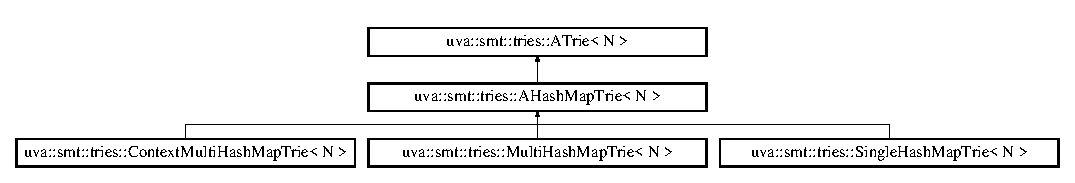
\includegraphics[height=2.007169cm]{classuva_1_1smt_1_1tries_1_1_a_hash_map_trie}
\end{center}
\end{figure}
\subsection*{Public Member Functions}
\begin{DoxyCompactItemize}
\item 
\hyperlink{classuva_1_1smt_1_1tries_1_1_a_hash_map_trie_a97fbb7a95590096e7416f82b2016998e}{A\+Hash\+Map\+Trie} (const float word\+Index\+Mem\+Factor)
\item 
virtual void \hyperlink{classuva_1_1smt_1_1tries_1_1_a_hash_map_trie_ad867b72350326f464b563fba6727ba5f}{pre\+Allocate} (const size\+\_\+t counts\mbox{[}N\mbox{]})
\item 
virtual \hyperlink{classuva_1_1smt_1_1tries_1_1_a_hash_map_trie_a5118f2f3566fd37b41998ef405ca6df1}{$\sim$\+A\+Hash\+Map\+Trie} ()
\end{DoxyCompactItemize}
\subsection*{Protected Member Functions}
\begin{DoxyCompactItemize}
\item 
\hyperlink{classuva_1_1smt_1_1tries_1_1_a_hash_map_trie_a42ba762f7a711f22111b3fefa46d418a}{A\+Hash\+Map\+Trie} (const \hyperlink{classuva_1_1smt_1_1tries_1_1_a_hash_map_trie}{A\+Hash\+Map\+Trie} \&orig)
\item 
const \hyperlink{namespaceuva_1_1smt_1_1hashing_acdc1f2765e669283f8e9c1ed42705314}{T\+Word\+Hash\+Size} \& \hyperlink{classuva_1_1smt_1_1tries_1_1_a_hash_map_trie_aa59ec4b6c4f0cb7eb4f1f4140bf9b9de}{get\+Back\+Off\+N\+Gram\+End\+Word\+Hash} ()
\item 
const \hyperlink{namespaceuva_1_1smt_1_1hashing_acdc1f2765e669283f8e9c1ed42705314}{T\+Word\+Hash\+Size} \& \hyperlink{classuva_1_1smt_1_1tries_1_1_a_hash_map_trie_a0c44c85dd64be9c9238d7313eb4dfcc9}{get\+N\+Gram\+End\+Word\+Hash} ()
\item 
void \hyperlink{classuva_1_1smt_1_1tries_1_1_a_hash_map_trie_a98254f0f1271f1651b3c70acbce8fcb3}{tokens\+To\+Hashes} (const vector$<$ string $>$ \&tokens, \hyperlink{namespaceuva_1_1smt_1_1hashing_acdc1f2765e669283f8e9c1ed42705314}{T\+Word\+Hash\+Size} word\+Hashes\mbox{[}N\mbox{]})
\item 
void \hyperlink{classuva_1_1smt_1_1tries_1_1_a_hash_map_trie_ababc583f0e22e3be69345bb43211fef6}{store\+N\+Gram\+Hashes} (const vector$<$ string $>$ \&ngram)
\item 
\hyperlink{namespaceuva_1_1smt_1_1hashing_a6cc10b288b11b76c718a898b022fbdd1}{T\+Reference\+Hash\+Size} \hyperlink{classuva_1_1smt_1_1tries_1_1_a_hash_map_trie_a1fb2b99ca8211bd45a343922b64cc96f}{compute\+Hash\+Context} (const \hyperlink{namespaceuva_1_1smt_1_1tries_a26064146e98856c7c4185efab0e61a36}{T\+Model\+Level} context\+Length, bool is\+Back\+Off)
\item 
{\footnotesize template$<$Logger\+::\+Debug\+Level log\+Level$>$ }\\\hyperlink{namespaceuva_1_1smt_1_1hashing_a6cc10b288b11b76c718a898b022fbdd1}{T\+Reference\+Hash\+Size} \hyperlink{classuva_1_1smt_1_1tries_1_1_a_hash_map_trie_a9a340430c87c0fb0725004689e8b47a0}{compute\+Hash\+Context} (const vector$<$ string $>$ \&tokens)
\item 
\hyperlink{namespaceuva_1_1smt_1_1hashing_acdc1f2765e669283f8e9c1ed42705314}{T\+Word\+Hash\+Size} \hyperlink{classuva_1_1smt_1_1tries_1_1_a_hash_map_trie_aae50ef05783fc3ca8367610475fe9b40}{get\+Unique\+Id\+Hash} (const string \&str)
\item 
\hyperlink{namespaceuva_1_1smt_1_1hashing_acdc1f2765e669283f8e9c1ed42705314}{T\+Word\+Hash\+Size} \hyperlink{classuva_1_1smt_1_1tries_1_1_a_hash_map_trie_ad23c5ad2dea14220aa3a61edcbd5346a}{create\+Unique\+Id\+Hash} (const string \&str)
\item 
void \hyperlink{classuva_1_1smt_1_1tries_1_1_a_hash_map_trie_af3f7c7d7f0c8dddd5fc2ea5318e58109}{record\+And\+Check} (const \hyperlink{namespaceuva_1_1smt_1_1hashing_acdc1f2765e669283f8e9c1ed42705314}{T\+Word\+Hash\+Size} word\+Hash, const \hyperlink{namespaceuva_1_1smt_1_1hashing_a6cc10b288b11b76c718a898b022fbdd1}{T\+Reference\+Hash\+Size} context\+Hash, const \hyperlink{structuva_1_1smt_1_1tries_1_1_s_back_off_n_gram}{S\+Back\+Off\+N\+Gram} \&gram) const 
\end{DoxyCompactItemize}
\subsection*{Static Protected Member Functions}
\begin{DoxyCompactItemize}
\item 
static \hyperlink{namespaceuva_1_1smt_1_1hashing_a6cc10b288b11b76c718a898b022fbdd1}{T\+Reference\+Hash\+Size} \hyperlink{classuva_1_1smt_1_1tries_1_1_a_hash_map_trie_af4aac18ab4f9db12bae8ba0ee8f63d92}{create\+Context} (\hyperlink{namespaceuva_1_1smt_1_1hashing_acdc1f2765e669283f8e9c1ed42705314}{T\+Word\+Hash\+Size} hash, \hyperlink{namespaceuva_1_1smt_1_1hashing_a6cc10b288b11b76c718a898b022fbdd1}{T\+Reference\+Hash\+Size} context)
\item 
static void \hyperlink{classuva_1_1smt_1_1tries_1_1_a_hash_map_trie_a9a35a764c83eafb369f7b858fa9b826e}{dessolve\+Context} (const \hyperlink{namespaceuva_1_1smt_1_1hashing_a6cc10b288b11b76c718a898b022fbdd1}{T\+Reference\+Hash\+Size} context, \hyperlink{namespaceuva_1_1smt_1_1hashing_acdc1f2765e669283f8e9c1ed42705314}{T\+Word\+Hash\+Size} \&sub\+Word, \hyperlink{namespaceuva_1_1smt_1_1hashing_a6cc10b288b11b76c718a898b022fbdd1}{T\+Reference\+Hash\+Size} \&sub\+Context)
\end{DoxyCompactItemize}


\subsection{Detailed Description}
\subsubsection*{template$<$T\+Model\+Level N$>$class uva\+::smt\+::tries\+::\+A\+Hash\+Map\+Trie$<$ N $>$}

This is a base abstract class for the Trie implementation using hash tables. The class only contains a few basic features, such as hashing functions and methods for working with the queued M-\/gram. 

\subsection{Constructor \& Destructor Documentation}
\hypertarget{classuva_1_1smt_1_1tries_1_1_a_hash_map_trie_a97fbb7a95590096e7416f82b2016998e}{}\index{uva\+::smt\+::tries\+::\+A\+Hash\+Map\+Trie@{uva\+::smt\+::tries\+::\+A\+Hash\+Map\+Trie}!A\+Hash\+Map\+Trie@{A\+Hash\+Map\+Trie}}
\index{A\+Hash\+Map\+Trie@{A\+Hash\+Map\+Trie}!uva\+::smt\+::tries\+::\+A\+Hash\+Map\+Trie@{uva\+::smt\+::tries\+::\+A\+Hash\+Map\+Trie}}
\subsubsection[{A\+Hash\+Map\+Trie(const float word\+Index\+Mem\+Factor)}]{\setlength{\rightskip}{0pt plus 5cm}template$<$T\+Model\+Level N$>$ {\bf uva\+::smt\+::tries\+::\+A\+Hash\+Map\+Trie}$<$ N $>$\+::{\bf A\+Hash\+Map\+Trie} (
\begin{DoxyParamCaption}
\item[{const float}]{word\+Index\+Mem\+Factor}
\end{DoxyParamCaption}
)\hspace{0.3cm}{\ttfamily [inline]}, {\ttfamily [explicit]}}\label{classuva_1_1smt_1_1tries_1_1_a_hash_map_trie_a97fbb7a95590096e7416f82b2016998e}
The basic class constructor, accepts memory factor(s) that are the coefficients used when pre-\/allocating memory for unordered maps.

If a factor is equal to 0.\+0 then no memory is pre-\/allocated. If the factor is equal to 1.\+0 then there is only as much preallocated as needed to store the gram entries. The latter is typically not enough as unordered\+\_\+map needs more memory for internal administration. If there is not enough memory pre-\/allocated then additional allocations will take place but it does not alway lead to more efficient memory usage. The observed behavior is that it is better to pre-\/allocate a bit more memory beforehand, than needed. This leads to less memory consumption. Depending on the type of unordered\+\_\+map key/value pair types the advised factor values are from 2.\+0 to 2.\+6. Because it can not be optimally determined beforehand, these are made constructor parameters so that they can be configured by the used. This breaks encapsulation a bit, exposing the internals, but there is no other better way, for fine tuning the memory usage.


\begin{DoxyParams}{Parameters}
{\em word\+Index\+Mem\+Factor} & the assigned memory factor for storage allocation in the unordered\+\_\+map used for the word index \\
\hline
\end{DoxyParams}
\hypertarget{classuva_1_1smt_1_1tries_1_1_a_hash_map_trie_a5118f2f3566fd37b41998ef405ca6df1}{}\index{uva\+::smt\+::tries\+::\+A\+Hash\+Map\+Trie@{uva\+::smt\+::tries\+::\+A\+Hash\+Map\+Trie}!````~A\+Hash\+Map\+Trie@{$\sim$\+A\+Hash\+Map\+Trie}}
\index{````~A\+Hash\+Map\+Trie@{$\sim$\+A\+Hash\+Map\+Trie}!uva\+::smt\+::tries\+::\+A\+Hash\+Map\+Trie@{uva\+::smt\+::tries\+::\+A\+Hash\+Map\+Trie}}
\subsubsection[{$\sim$\+A\+Hash\+Map\+Trie()}]{\setlength{\rightskip}{0pt plus 5cm}template$<$T\+Model\+Level N$>$ virtual {\bf uva\+::smt\+::tries\+::\+A\+Hash\+Map\+Trie}$<$ N $>$\+::$\sim${\bf A\+Hash\+Map\+Trie} (
\begin{DoxyParamCaption}
{}
\end{DoxyParamCaption}
)\hspace{0.3cm}{\ttfamily [inline]}, {\ttfamily [virtual]}}\label{classuva_1_1smt_1_1tries_1_1_a_hash_map_trie_a5118f2f3566fd37b41998ef405ca6df1}
The basic class destructor \hypertarget{classuva_1_1smt_1_1tries_1_1_a_hash_map_trie_a42ba762f7a711f22111b3fefa46d418a}{}\index{uva\+::smt\+::tries\+::\+A\+Hash\+Map\+Trie@{uva\+::smt\+::tries\+::\+A\+Hash\+Map\+Trie}!A\+Hash\+Map\+Trie@{A\+Hash\+Map\+Trie}}
\index{A\+Hash\+Map\+Trie@{A\+Hash\+Map\+Trie}!uva\+::smt\+::tries\+::\+A\+Hash\+Map\+Trie@{uva\+::smt\+::tries\+::\+A\+Hash\+Map\+Trie}}
\subsubsection[{A\+Hash\+Map\+Trie(const A\+Hash\+Map\+Trie \&orig)}]{\setlength{\rightskip}{0pt plus 5cm}template$<$T\+Model\+Level N$>$ {\bf uva\+::smt\+::tries\+::\+A\+Hash\+Map\+Trie}$<$ N $>$\+::{\bf A\+Hash\+Map\+Trie} (
\begin{DoxyParamCaption}
\item[{const {\bf A\+Hash\+Map\+Trie}$<$ N $>$ \&}]{orig}
\end{DoxyParamCaption}
)\hspace{0.3cm}{\ttfamily [inline]}, {\ttfamily [protected]}}\label{classuva_1_1smt_1_1tries_1_1_a_hash_map_trie_a42ba762f7a711f22111b3fefa46d418a}
The copy constructor, is made private as we do not intend to copy this class objects 
\begin{DoxyParams}{Parameters}
{\em orig} & the object to copy from \\
\hline
\end{DoxyParams}


\subsection{Member Function Documentation}
\hypertarget{classuva_1_1smt_1_1tries_1_1_a_hash_map_trie_a1fb2b99ca8211bd45a343922b64cc96f}{}\index{uva\+::smt\+::tries\+::\+A\+Hash\+Map\+Trie@{uva\+::smt\+::tries\+::\+A\+Hash\+Map\+Trie}!compute\+Hash\+Context@{compute\+Hash\+Context}}
\index{compute\+Hash\+Context@{compute\+Hash\+Context}!uva\+::smt\+::tries\+::\+A\+Hash\+Map\+Trie@{uva\+::smt\+::tries\+::\+A\+Hash\+Map\+Trie}}
\subsubsection[{compute\+Hash\+Context(const T\+Model\+Level context\+Length, bool is\+Back\+Off)}]{\setlength{\rightskip}{0pt plus 5cm}template$<$T\+Model\+Level N$>$ {\bf T\+Reference\+Hash\+Size} {\bf uva\+::smt\+::tries\+::\+A\+Hash\+Map\+Trie}$<$ N $>$\+::compute\+Hash\+Context (
\begin{DoxyParamCaption}
\item[{const {\bf T\+Model\+Level}}]{context\+Length, }
\item[{bool}]{is\+Back\+Off}
\end{DoxyParamCaption}
)\hspace{0.3cm}{\ttfamily [inline]}, {\ttfamily [protected]}}\label{classuva_1_1smt_1_1tries_1_1_a_hash_map_trie_a1fb2b99ca8211bd45a343922b64cc96f}
Compute the context hash for the M-\/\+Gram prefix, example\+:

N = 5

0 1 2 3 4 w1 w2 w3 w4 w5

context\+Length = 2

0 1 2 3 4 w1 w2 w3 w4 w5 $^\wedge$ $^\wedge$ Hash will be computed for the 3-\/gram prefix w3 w4.


\begin{DoxyParams}{Parameters}
{\em context\+Length} & the length of the context to compute \\
\hline
{\em is\+Back\+Off} & is the boolean flag that determines whether we compute the context for the entire M-\/\+Gram or for the back-\/off sub-\/\+M-\/gram. For the latter we consider w1 w2 w3 w4 only \\
\hline
\end{DoxyParams}
\begin{DoxyReturn}{Returns}
the computed hash context 
\end{DoxyReturn}
\hypertarget{classuva_1_1smt_1_1tries_1_1_a_hash_map_trie_a9a340430c87c0fb0725004689e8b47a0}{}\index{uva\+::smt\+::tries\+::\+A\+Hash\+Map\+Trie@{uva\+::smt\+::tries\+::\+A\+Hash\+Map\+Trie}!compute\+Hash\+Context@{compute\+Hash\+Context}}
\index{compute\+Hash\+Context@{compute\+Hash\+Context}!uva\+::smt\+::tries\+::\+A\+Hash\+Map\+Trie@{uva\+::smt\+::tries\+::\+A\+Hash\+Map\+Trie}}
\subsubsection[{compute\+Hash\+Context(const vector$<$ string $>$ \&tokens)}]{\setlength{\rightskip}{0pt plus 5cm}template$<$T\+Model\+Level N$>$ template$<$Logger\+::\+Debug\+Level log\+Level$>$ {\bf T\+Reference\+Hash\+Size} {\bf uva\+::smt\+::tries\+::\+A\+Hash\+Map\+Trie}$<$ N $>$\+::compute\+Hash\+Context (
\begin{DoxyParamCaption}
\item[{const vector$<$ string $>$ \&}]{tokens}
\end{DoxyParamCaption}
)\hspace{0.3cm}{\ttfamily [inline]}, {\ttfamily [protected]}}\label{classuva_1_1smt_1_1tries_1_1_a_hash_map_trie_a9a340430c87c0fb0725004689e8b47a0}
This function computes the hash context of the N-\/gram given by the tokens, e.\+g. \mbox{[}w1 w2 w3 w4\mbox{]} 
\begin{DoxyParams}{Parameters}
{\em tokens} & the N-\/gram tokens \\
\hline
\end{DoxyParams}
\begin{DoxyReturn}{Returns}
the resulting hash of the context(w1 w2 w3) or U\+N\+D\+E\+F\+I\+N\+E\+D\+\_\+\+W\+O\+R\+D\+\_\+\+H\+A\+S\+H for any M-\/\+Gram with M $<$= 1 
\end{DoxyReturn}
\hypertarget{classuva_1_1smt_1_1tries_1_1_a_hash_map_trie_af4aac18ab4f9db12bae8ba0ee8f63d92}{}\index{uva\+::smt\+::tries\+::\+A\+Hash\+Map\+Trie@{uva\+::smt\+::tries\+::\+A\+Hash\+Map\+Trie}!create\+Context@{create\+Context}}
\index{create\+Context@{create\+Context}!uva\+::smt\+::tries\+::\+A\+Hash\+Map\+Trie@{uva\+::smt\+::tries\+::\+A\+Hash\+Map\+Trie}}
\subsubsection[{create\+Context(\+T\+Word\+Hash\+Size hash, T\+Reference\+Hash\+Size context)}]{\setlength{\rightskip}{0pt plus 5cm}template$<$T\+Model\+Level N$>$ static {\bf T\+Reference\+Hash\+Size} {\bf uva\+::smt\+::tries\+::\+A\+Hash\+Map\+Trie}$<$ N $>$\+::create\+Context (
\begin{DoxyParamCaption}
\item[{{\bf T\+Word\+Hash\+Size}}]{hash, }
\item[{{\bf T\+Reference\+Hash\+Size}}]{context}
\end{DoxyParamCaption}
)\hspace{0.3cm}{\ttfamily [inline]}, {\ttfamily [static]}, {\ttfamily [protected]}}\label{classuva_1_1smt_1_1tries_1_1_a_hash_map_trie_af4aac18ab4f9db12bae8ba0ee8f63d92}
Computes the N-\/\+Gram context using the previous context and the current word hash 
\begin{DoxyParams}{Parameters}
{\em hash} & the current word hash \\
\hline
{\em context} & the previous context \\
\hline
\end{DoxyParams}
\begin{DoxyReturn}{Returns}
the resulting context 
\end{DoxyReturn}
\hypertarget{classuva_1_1smt_1_1tries_1_1_a_hash_map_trie_ad23c5ad2dea14220aa3a61edcbd5346a}{}\index{uva\+::smt\+::tries\+::\+A\+Hash\+Map\+Trie@{uva\+::smt\+::tries\+::\+A\+Hash\+Map\+Trie}!create\+Unique\+Id\+Hash@{create\+Unique\+Id\+Hash}}
\index{create\+Unique\+Id\+Hash@{create\+Unique\+Id\+Hash}!uva\+::smt\+::tries\+::\+A\+Hash\+Map\+Trie@{uva\+::smt\+::tries\+::\+A\+Hash\+Map\+Trie}}
\subsubsection[{create\+Unique\+Id\+Hash(const string \&str)}]{\setlength{\rightskip}{0pt plus 5cm}template$<$T\+Model\+Level N$>$ {\bf T\+Word\+Hash\+Size} {\bf uva\+::smt\+::tries\+::\+A\+Hash\+Map\+Trie}$<$ N $>$\+::create\+Unique\+Id\+Hash (
\begin{DoxyParamCaption}
\item[{const string \&}]{str}
\end{DoxyParamCaption}
)\hspace{0.3cm}{\ttfamily [inline]}, {\ttfamily [protected]}}\label{classuva_1_1smt_1_1tries_1_1_a_hash_map_trie_ad23c5ad2dea14220aa3a61edcbd5346a}
This function creates/gets a hash for the given word. Note\+: The hash id will be unique! 
\begin{DoxyParams}{Parameters}
{\em str} & the word to hash \\
\hline
\end{DoxyParams}
\begin{DoxyReturn}{Returns}
the resulting hash 
\end{DoxyReturn}
\hypertarget{classuva_1_1smt_1_1tries_1_1_a_hash_map_trie_a9a35a764c83eafb369f7b858fa9b826e}{}\index{uva\+::smt\+::tries\+::\+A\+Hash\+Map\+Trie@{uva\+::smt\+::tries\+::\+A\+Hash\+Map\+Trie}!dessolve\+Context@{dessolve\+Context}}
\index{dessolve\+Context@{dessolve\+Context}!uva\+::smt\+::tries\+::\+A\+Hash\+Map\+Trie@{uva\+::smt\+::tries\+::\+A\+Hash\+Map\+Trie}}
\subsubsection[{dessolve\+Context(const T\+Reference\+Hash\+Size context, T\+Word\+Hash\+Size \&sub\+Word, T\+Reference\+Hash\+Size \&sub\+Context)}]{\setlength{\rightskip}{0pt plus 5cm}template$<$T\+Model\+Level N$>$ static void {\bf uva\+::smt\+::tries\+::\+A\+Hash\+Map\+Trie}$<$ N $>$\+::dessolve\+Context (
\begin{DoxyParamCaption}
\item[{const {\bf T\+Reference\+Hash\+Size}}]{context, }
\item[{{\bf T\+Word\+Hash\+Size} \&}]{sub\+Word, }
\item[{{\bf T\+Reference\+Hash\+Size} \&}]{sub\+Context}
\end{DoxyParamCaption}
)\hspace{0.3cm}{\ttfamily [inline]}, {\ttfamily [static]}, {\ttfamily [protected]}}\label{classuva_1_1smt_1_1tries_1_1_a_hash_map_trie_a9a35a764c83eafb369f7b858fa9b826e}
This function dissolves the given Ngram context (for N$>$=2) into a sub-\/word hash and a sub-\/context\+: c(w\+\_\+n) is defined by hash(w\+\_\+n) and c(w\+\_\+(n-\/1)) 
\begin{DoxyParams}{Parameters}
{\em context} & the given context to dissolve \\
\hline
{\em sub\+Word} & the sub-\/work \\
\hline
{\em sub\+Context} & the sub-\/context \\
\hline
\end{DoxyParams}
\hypertarget{classuva_1_1smt_1_1tries_1_1_a_hash_map_trie_aa59ec4b6c4f0cb7eb4f1f4140bf9b9de}{}\index{uva\+::smt\+::tries\+::\+A\+Hash\+Map\+Trie@{uva\+::smt\+::tries\+::\+A\+Hash\+Map\+Trie}!get\+Back\+Off\+N\+Gram\+End\+Word\+Hash@{get\+Back\+Off\+N\+Gram\+End\+Word\+Hash}}
\index{get\+Back\+Off\+N\+Gram\+End\+Word\+Hash@{get\+Back\+Off\+N\+Gram\+End\+Word\+Hash}!uva\+::smt\+::tries\+::\+A\+Hash\+Map\+Trie@{uva\+::smt\+::tries\+::\+A\+Hash\+Map\+Trie}}
\subsubsection[{get\+Back\+Off\+N\+Gram\+End\+Word\+Hash()}]{\setlength{\rightskip}{0pt plus 5cm}template$<$T\+Model\+Level N$>$ const {\bf T\+Word\+Hash\+Size}\& {\bf uva\+::smt\+::tries\+::\+A\+Hash\+Map\+Trie}$<$ N $>$\+::get\+Back\+Off\+N\+Gram\+End\+Word\+Hash (
\begin{DoxyParamCaption}
{}
\end{DoxyParamCaption}
)\hspace{0.3cm}{\ttfamily [inline]}, {\ttfamily [protected]}}\label{classuva_1_1smt_1_1tries_1_1_a_hash_map_trie_aa59ec4b6c4f0cb7eb4f1f4140bf9b9de}
Gets the word hash for the end word of the back-\/off N-\/\+Gram \begin{DoxyReturn}{Returns}
the word hash for the end word of the back-\/off N-\/\+Gram 
\end{DoxyReturn}
\hypertarget{classuva_1_1smt_1_1tries_1_1_a_hash_map_trie_a0c44c85dd64be9c9238d7313eb4dfcc9}{}\index{uva\+::smt\+::tries\+::\+A\+Hash\+Map\+Trie@{uva\+::smt\+::tries\+::\+A\+Hash\+Map\+Trie}!get\+N\+Gram\+End\+Word\+Hash@{get\+N\+Gram\+End\+Word\+Hash}}
\index{get\+N\+Gram\+End\+Word\+Hash@{get\+N\+Gram\+End\+Word\+Hash}!uva\+::smt\+::tries\+::\+A\+Hash\+Map\+Trie@{uva\+::smt\+::tries\+::\+A\+Hash\+Map\+Trie}}
\subsubsection[{get\+N\+Gram\+End\+Word\+Hash()}]{\setlength{\rightskip}{0pt plus 5cm}template$<$T\+Model\+Level N$>$ const {\bf T\+Word\+Hash\+Size}\& {\bf uva\+::smt\+::tries\+::\+A\+Hash\+Map\+Trie}$<$ N $>$\+::get\+N\+Gram\+End\+Word\+Hash (
\begin{DoxyParamCaption}
{}
\end{DoxyParamCaption}
)\hspace{0.3cm}{\ttfamily [inline]}, {\ttfamily [protected]}}\label{classuva_1_1smt_1_1tries_1_1_a_hash_map_trie_a0c44c85dd64be9c9238d7313eb4dfcc9}
Gets the word hash for the last word in the N-\/gram \begin{DoxyReturn}{Returns}
the word hash for the last word in the N-\/gram 
\end{DoxyReturn}
\hypertarget{classuva_1_1smt_1_1tries_1_1_a_hash_map_trie_aae50ef05783fc3ca8367610475fe9b40}{}\index{uva\+::smt\+::tries\+::\+A\+Hash\+Map\+Trie@{uva\+::smt\+::tries\+::\+A\+Hash\+Map\+Trie}!get\+Unique\+Id\+Hash@{get\+Unique\+Id\+Hash}}
\index{get\+Unique\+Id\+Hash@{get\+Unique\+Id\+Hash}!uva\+::smt\+::tries\+::\+A\+Hash\+Map\+Trie@{uva\+::smt\+::tries\+::\+A\+Hash\+Map\+Trie}}
\subsubsection[{get\+Unique\+Id\+Hash(const string \&str)}]{\setlength{\rightskip}{0pt plus 5cm}template$<$T\+Model\+Level N$>$ {\bf T\+Word\+Hash\+Size} {\bf uva\+::smt\+::tries\+::\+A\+Hash\+Map\+Trie}$<$ N $>$\+::get\+Unique\+Id\+Hash (
\begin{DoxyParamCaption}
\item[{const string \&}]{str}
\end{DoxyParamCaption}
)\hspace{0.3cm}{\ttfamily [inline]}, {\ttfamily [protected]}}\label{classuva_1_1smt_1_1tries_1_1_a_hash_map_trie_aae50ef05783fc3ca8367610475fe9b40}
This function gets a hash for the given word word based no the stored 1-\/\+Grams. If the word is not known then an unknown word I\+D is returned\+: U\+N\+K\+N\+O\+W\+N\+\_\+\+W\+O\+R\+D\+\_\+\+H\+A\+S\+H 
\begin{DoxyParams}{Parameters}
{\em str} & the word to hash \\
\hline
\end{DoxyParams}
\begin{DoxyReturn}{Returns}
the resulting hash 
\end{DoxyReturn}
\hypertarget{classuva_1_1smt_1_1tries_1_1_a_hash_map_trie_ad867b72350326f464b563fba6727ba5f}{}\index{uva\+::smt\+::tries\+::\+A\+Hash\+Map\+Trie@{uva\+::smt\+::tries\+::\+A\+Hash\+Map\+Trie}!pre\+Allocate@{pre\+Allocate}}
\index{pre\+Allocate@{pre\+Allocate}!uva\+::smt\+::tries\+::\+A\+Hash\+Map\+Trie@{uva\+::smt\+::tries\+::\+A\+Hash\+Map\+Trie}}
\subsubsection[{pre\+Allocate(const size\+\_\+t counts[N])}]{\setlength{\rightskip}{0pt plus 5cm}template$<$T\+Model\+Level N$>$ virtual void {\bf uva\+::smt\+::tries\+::\+A\+Hash\+Map\+Trie}$<$ N $>$\+::pre\+Allocate (
\begin{DoxyParamCaption}
\item[{const size\+\_\+t}]{counts\mbox{[}\+N\mbox{]}}
\end{DoxyParamCaption}
)\hspace{0.3cm}{\ttfamily [inline]}, {\ttfamily [virtual]}}\label{classuva_1_1smt_1_1tries_1_1_a_hash_map_trie_ad867b72350326f464b563fba6727ba5f}
The defaul implementation that pre-\/allocates the word\+Index 
\begin{DoxyParams}{Parameters}
{\em counts} & the number of ngrams \\
\hline
\end{DoxyParams}


Implements \hyperlink{classuva_1_1smt_1_1tries_1_1_a_trie_a642f48565e195a41a768b2cfa247735a}{uva\+::smt\+::tries\+::\+A\+Trie$<$ N $>$}.



Reimplemented in \hyperlink{classuva_1_1smt_1_1tries_1_1_context_multi_hash_map_trie_ac744e6f6e63317d1f955ac96d504f724}{uva\+::smt\+::tries\+::\+Context\+Multi\+Hash\+Map\+Trie$<$ N $>$}, \hyperlink{classuva_1_1smt_1_1tries_1_1_multi_hash_map_trie_ac7d916356f0ad36d33c0c4722e6459b9}{uva\+::smt\+::tries\+::\+Multi\+Hash\+Map\+Trie$<$ N $>$}, and \hyperlink{classuva_1_1smt_1_1tries_1_1_single_hash_map_trie_a6a40f4047280dedc7f402d6502547b2c}{uva\+::smt\+::tries\+::\+Single\+Hash\+Map\+Trie$<$ N $>$}.

\hypertarget{classuva_1_1smt_1_1tries_1_1_a_hash_map_trie_af3f7c7d7f0c8dddd5fc2ea5318e58109}{}\index{uva\+::smt\+::tries\+::\+A\+Hash\+Map\+Trie@{uva\+::smt\+::tries\+::\+A\+Hash\+Map\+Trie}!record\+And\+Check@{record\+And\+Check}}
\index{record\+And\+Check@{record\+And\+Check}!uva\+::smt\+::tries\+::\+A\+Hash\+Map\+Trie@{uva\+::smt\+::tries\+::\+A\+Hash\+Map\+Trie}}
\subsubsection[{record\+And\+Check(const T\+Word\+Hash\+Size word\+Hash, const T\+Reference\+Hash\+Size context\+Hash, const S\+Back\+Off\+N\+Gram \&gram) const }]{\setlength{\rightskip}{0pt plus 5cm}template$<$T\+Model\+Level N$>$ void {\bf uva\+::smt\+::tries\+::\+A\+Hash\+Map\+Trie}$<$ N $>$\+::record\+And\+Check (
\begin{DoxyParamCaption}
\item[{const {\bf T\+Word\+Hash\+Size}}]{word\+Hash, }
\item[{const {\bf T\+Reference\+Hash\+Size}}]{context\+Hash, }
\item[{const {\bf S\+Back\+Off\+N\+Gram} \&}]{gram}
\end{DoxyParamCaption}
) const\hspace{0.3cm}{\ttfamily [inline]}, {\ttfamily [protected]}}\label{classuva_1_1smt_1_1tries_1_1_a_hash_map_trie_af3f7c7d7f0c8dddd5fc2ea5318e58109}
\hypertarget{classuva_1_1smt_1_1tries_1_1_a_hash_map_trie_ababc583f0e22e3be69345bb43211fef6}{}\index{uva\+::smt\+::tries\+::\+A\+Hash\+Map\+Trie@{uva\+::smt\+::tries\+::\+A\+Hash\+Map\+Trie}!store\+N\+Gram\+Hashes@{store\+N\+Gram\+Hashes}}
\index{store\+N\+Gram\+Hashes@{store\+N\+Gram\+Hashes}!uva\+::smt\+::tries\+::\+A\+Hash\+Map\+Trie@{uva\+::smt\+::tries\+::\+A\+Hash\+Map\+Trie}}
\subsubsection[{store\+N\+Gram\+Hashes(const vector$<$ string $>$ \&ngram)}]{\setlength{\rightskip}{0pt plus 5cm}template$<$T\+Model\+Level N$>$ void {\bf uva\+::smt\+::tries\+::\+A\+Hash\+Map\+Trie}$<$ N $>$\+::store\+N\+Gram\+Hashes (
\begin{DoxyParamCaption}
\item[{const vector$<$ string $>$ \&}]{ngram}
\end{DoxyParamCaption}
)\hspace{0.3cm}{\ttfamily [inline]}, {\ttfamily [protected]}}\label{classuva_1_1smt_1_1tries_1_1_a_hash_map_trie_ababc583f0e22e3be69345bb43211fef6}
Converts the given tokens to hashes and stores it in m\+Gram\+Word\+Hashes 
\begin{DoxyParams}{Parameters}
{\em ngram} & the n-\/gram tokens to convert to hashes \\
\hline
\end{DoxyParams}
\hypertarget{classuva_1_1smt_1_1tries_1_1_a_hash_map_trie_a98254f0f1271f1651b3c70acbce8fcb3}{}\index{uva\+::smt\+::tries\+::\+A\+Hash\+Map\+Trie@{uva\+::smt\+::tries\+::\+A\+Hash\+Map\+Trie}!tokens\+To\+Hashes@{tokens\+To\+Hashes}}
\index{tokens\+To\+Hashes@{tokens\+To\+Hashes}!uva\+::smt\+::tries\+::\+A\+Hash\+Map\+Trie@{uva\+::smt\+::tries\+::\+A\+Hash\+Map\+Trie}}
\subsubsection[{tokens\+To\+Hashes(const vector$<$ string $>$ \&tokens, T\+Word\+Hash\+Size word\+Hashes[N])}]{\setlength{\rightskip}{0pt plus 5cm}template$<$T\+Model\+Level N$>$ void {\bf uva\+::smt\+::tries\+::\+A\+Hash\+Map\+Trie}$<$ N $>$\+::tokens\+To\+Hashes (
\begin{DoxyParamCaption}
\item[{const vector$<$ string $>$ \&}]{tokens, }
\item[{{\bf T\+Word\+Hash\+Size}}]{word\+Hashes\mbox{[}\+N\mbox{]}}
\end{DoxyParamCaption}
)\hspace{0.3cm}{\ttfamily [inline]}, {\ttfamily [protected]}}\label{classuva_1_1smt_1_1tries_1_1_a_hash_map_trie_a98254f0f1271f1651b3c70acbce8fcb3}
This method converts the M-\/\+Gram tokens into hashes and stores them in an array. Note that, M is the size of the tokens array. It is not checked, for the sake of performance but is assumed that M is $<$= N! 
\begin{DoxyParams}{Parameters}
{\em tokens} & the tokens to be transformed into word hashes must have size $<$=N \\
\hline
{\em word\+Hashes} & the out array parameter to store the hashes. \\
\hline
\end{DoxyParams}


The documentation for this class was generated from the following file\+:\begin{DoxyCompactItemize}
\item 
inc/\hyperlink{_a_hash_map_trie_8hpp}{A\+Hash\+Map\+Trie.\+hpp}\end{DoxyCompactItemize}

\hypertarget{classuva_1_1smt_1_1tries_1_1arpa_1_1_a_r_p_a_gram_builder}{}\section{uva\+:\+:smt\+:\+:tries\+:\+:arpa\+:\+:A\+R\+P\+A\+Gram\+Builder Class Reference}
\label{classuva_1_1smt_1_1tries_1_1arpa_1_1_a_r_p_a_gram_builder}\index{uva\+::smt\+::tries\+::arpa\+::\+A\+R\+P\+A\+Gram\+Builder@{uva\+::smt\+::tries\+::arpa\+::\+A\+R\+P\+A\+Gram\+Builder}}


{\ttfamily \#include $<$A\+R\+P\+A\+Gram\+Builder.\+hpp$>$}

\subsection*{Public Member Functions}
\begin{DoxyCompactItemize}
\item 
\hyperlink{classuva_1_1smt_1_1tries_1_1arpa_1_1_a_r_p_a_gram_builder_aabc607c9ba43ff636456b23cb8236e60}{A\+R\+P\+A\+Gram\+Builder} (const \hyperlink{namespaceuva_1_1smt_1_1tries_a26064146e98856c7c4185efab0e61a36}{T\+Model\+Level} level, \hyperlink{namespaceuva_1_1smt_1_1tries_1_1arpa_a16805e23db5ab5a826e46ae4a59a0a71}{T\+Add\+Gram\+Funct} add\+Garm\+Func, const char delim)
\item 
bool \hyperlink{classuva_1_1smt_1_1tries_1_1arpa_1_1_a_r_p_a_gram_builder_af505ce38243a3e39fbc6b4d9ee83368f}{process\+String} (const string \&data)
\item 
virtual \hyperlink{classuva_1_1smt_1_1tries_1_1arpa_1_1_a_r_p_a_gram_builder_ab65614501c700f5654ddd3397050e671}{$\sim$\+A\+R\+P\+A\+Gram\+Builder} ()
\end{DoxyCompactItemize}
\subsection*{Protected Member Functions}
\begin{DoxyCompactItemize}
\item 
\hyperlink{classuva_1_1smt_1_1tries_1_1arpa_1_1_a_r_p_a_gram_builder_ad9de06a743ac014b818df81d2bec0267}{A\+R\+P\+A\+Gram\+Builder} (const \hyperlink{classuva_1_1smt_1_1tries_1_1arpa_1_1_a_r_p_a_gram_builder}{A\+R\+P\+A\+Gram\+Builder} \&orig)
\end{DoxyCompactItemize}
\subsection*{Protected Attributes}
\begin{DoxyCompactItemize}
\item 
\hyperlink{namespaceuva_1_1smt_1_1tries_1_1arpa_a16805e23db5ab5a826e46ae4a59a0a71}{T\+Add\+Gram\+Funct} \hyperlink{classuva_1_1smt_1_1tries_1_1arpa_1_1_a_r_p_a_gram_builder_aff22fce8a9b8b5f00e5d9fcad4dd218c}{\+\_\+add\+Garm\+Func}
\item 
const char \hyperlink{classuva_1_1smt_1_1tries_1_1arpa_1_1_a_r_p_a_gram_builder_a21ec180396f89d3a252fdd750217c2b7}{\+\_\+delim}
\item 
const \hyperlink{namespaceuva_1_1smt_1_1tries_a26064146e98856c7c4185efab0e61a36}{T\+Model\+Level} \hyperlink{classuva_1_1smt_1_1tries_1_1arpa_1_1_a_r_p_a_gram_builder_a333c47efee11f1812378325732d0e43c}{\+\_\+level}
\item 
\hyperlink{structuva_1_1smt_1_1tries_1_1_s_back_off_n_gram}{S\+Back\+Off\+N\+Gram} \hyperlink{classuva_1_1smt_1_1tries_1_1arpa_1_1_a_r_p_a_gram_builder_adcf89e815cdffc79ada87f33d8ebfb74}{\+\_\+ngram}
\item 
const uint \hyperlink{classuva_1_1smt_1_1tries_1_1arpa_1_1_a_r_p_a_gram_builder_a6ab807fa7fd956beabb58d8f275050d0}{M\+I\+N\+\_\+\+N\+U\+M\+\_\+\+T\+O\+K\+E\+N\+S\+\_\+\+N\+G\+R\+A\+M\+\_\+\+S\+T\+R}
\item 
const uint \hyperlink{classuva_1_1smt_1_1tries_1_1arpa_1_1_a_r_p_a_gram_builder_afd40395f976805a4835bc0b03e26cee2}{M\+A\+X\+\_\+\+N\+U\+M\+\_\+\+T\+O\+K\+E\+N\+S\+\_\+\+N\+G\+R\+A\+M\+\_\+\+S\+T\+R}
\end{DoxyCompactItemize}


\subsection{Detailed Description}
This class is responsible for splitting a piece of text in a number of ngrams and place it into the trie 

\subsection{Constructor \& Destructor Documentation}
\hypertarget{classuva_1_1smt_1_1tries_1_1arpa_1_1_a_r_p_a_gram_builder_aabc607c9ba43ff636456b23cb8236e60}{}\index{uva\+::smt\+::tries\+::arpa\+::\+A\+R\+P\+A\+Gram\+Builder@{uva\+::smt\+::tries\+::arpa\+::\+A\+R\+P\+A\+Gram\+Builder}!A\+R\+P\+A\+Gram\+Builder@{A\+R\+P\+A\+Gram\+Builder}}
\index{A\+R\+P\+A\+Gram\+Builder@{A\+R\+P\+A\+Gram\+Builder}!uva\+::smt\+::tries\+::arpa\+::\+A\+R\+P\+A\+Gram\+Builder@{uva\+::smt\+::tries\+::arpa\+::\+A\+R\+P\+A\+Gram\+Builder}}
\subsubsection[{A\+R\+P\+A\+Gram\+Builder(const T\+Model\+Level level, T\+Add\+Gram\+Funct add\+Garm\+Func, const char delim)}]{\setlength{\rightskip}{0pt plus 5cm}uva\+::smt\+::tries\+::arpa\+::\+A\+R\+P\+A\+Gram\+Builder\+::\+A\+R\+P\+A\+Gram\+Builder (
\begin{DoxyParamCaption}
\item[{const {\bf T\+Model\+Level}}]{level, }
\item[{{\bf T\+Add\+Gram\+Funct}}]{add\+Garm\+Func, }
\item[{const char}]{delim}
\end{DoxyParamCaption}
)}\label{classuva_1_1smt_1_1tries_1_1arpa_1_1_a_r_p_a_gram_builder_aabc607c9ba43ff636456b23cb8236e60}
The constructor to be used in order to instantiate a N-\/\+Gram builder 
\begin{DoxyParams}{Parameters}
{\em level} & the level of the N-\/grams to be processed \\
\hline
{\em add\+Garm\+Func} & the strategy for adding the N-\/grams \\
\hline
{\em delim} & the delimiter for the N-\/gram string \\
\hline
\end{DoxyParams}
\hypertarget{classuva_1_1smt_1_1tries_1_1arpa_1_1_a_r_p_a_gram_builder_ab65614501c700f5654ddd3397050e671}{}\index{uva\+::smt\+::tries\+::arpa\+::\+A\+R\+P\+A\+Gram\+Builder@{uva\+::smt\+::tries\+::arpa\+::\+A\+R\+P\+A\+Gram\+Builder}!````~A\+R\+P\+A\+Gram\+Builder@{$\sim$\+A\+R\+P\+A\+Gram\+Builder}}
\index{````~A\+R\+P\+A\+Gram\+Builder@{$\sim$\+A\+R\+P\+A\+Gram\+Builder}!uva\+::smt\+::tries\+::arpa\+::\+A\+R\+P\+A\+Gram\+Builder@{uva\+::smt\+::tries\+::arpa\+::\+A\+R\+P\+A\+Gram\+Builder}}
\subsubsection[{$\sim$\+A\+R\+P\+A\+Gram\+Builder()}]{\setlength{\rightskip}{0pt plus 5cm}uva\+::smt\+::tries\+::arpa\+::\+A\+R\+P\+A\+Gram\+Builder\+::$\sim$\+A\+R\+P\+A\+Gram\+Builder (
\begin{DoxyParamCaption}
{}
\end{DoxyParamCaption}
)\hspace{0.3cm}{\ttfamily [virtual]}}\label{classuva_1_1smt_1_1tries_1_1arpa_1_1_a_r_p_a_gram_builder_ab65614501c700f5654ddd3397050e671}
\hypertarget{classuva_1_1smt_1_1tries_1_1arpa_1_1_a_r_p_a_gram_builder_ad9de06a743ac014b818df81d2bec0267}{}\index{uva\+::smt\+::tries\+::arpa\+::\+A\+R\+P\+A\+Gram\+Builder@{uva\+::smt\+::tries\+::arpa\+::\+A\+R\+P\+A\+Gram\+Builder}!A\+R\+P\+A\+Gram\+Builder@{A\+R\+P\+A\+Gram\+Builder}}
\index{A\+R\+P\+A\+Gram\+Builder@{A\+R\+P\+A\+Gram\+Builder}!uva\+::smt\+::tries\+::arpa\+::\+A\+R\+P\+A\+Gram\+Builder@{uva\+::smt\+::tries\+::arpa\+::\+A\+R\+P\+A\+Gram\+Builder}}
\subsubsection[{A\+R\+P\+A\+Gram\+Builder(const A\+R\+P\+A\+Gram\+Builder \&orig)}]{\setlength{\rightskip}{0pt plus 5cm}uva\+::smt\+::tries\+::arpa\+::\+A\+R\+P\+A\+Gram\+Builder\+::\+A\+R\+P\+A\+Gram\+Builder (
\begin{DoxyParamCaption}
\item[{const {\bf A\+R\+P\+A\+Gram\+Builder} \&}]{orig}
\end{DoxyParamCaption}
)\hspace{0.3cm}{\ttfamily [protected]}}\label{classuva_1_1smt_1_1tries_1_1arpa_1_1_a_r_p_a_gram_builder_ad9de06a743ac014b818df81d2bec0267}
The copy constructor 
\begin{DoxyParams}{Parameters}
{\em orig} & the other builder to copy \\
\hline
\end{DoxyParams}


\subsection{Member Function Documentation}
\hypertarget{classuva_1_1smt_1_1tries_1_1arpa_1_1_a_r_p_a_gram_builder_af505ce38243a3e39fbc6b4d9ee83368f}{}\index{uva\+::smt\+::tries\+::arpa\+::\+A\+R\+P\+A\+Gram\+Builder@{uva\+::smt\+::tries\+::arpa\+::\+A\+R\+P\+A\+Gram\+Builder}!process\+String@{process\+String}}
\index{process\+String@{process\+String}!uva\+::smt\+::tries\+::arpa\+::\+A\+R\+P\+A\+Gram\+Builder@{uva\+::smt\+::tries\+::arpa\+::\+A\+R\+P\+A\+Gram\+Builder}}
\subsubsection[{process\+String(const string \&data)}]{\setlength{\rightskip}{0pt plus 5cm}bool uva\+::smt\+::tries\+::arpa\+::\+A\+R\+P\+A\+Gram\+Builder\+::process\+String (
\begin{DoxyParamCaption}
\item[{const string \&}]{data}
\end{DoxyParamCaption}
)}\label{classuva_1_1smt_1_1tries_1_1arpa_1_1_a_r_p_a_gram_builder_af505ce38243a3e39fbc6b4d9ee83368f}
This pure virtual method is supposed to parse the N-\/\+Gram string from the A\+R\+P\+A file format of a Back-\/\+Off language model and then add the obtained data to the Trie. This method has a default implementation that should work for N-\/grams with level $>$ M\+I\+N\+\_\+\+N\+G\+R\+A\+M\+\_\+\+L\+E\+V\+E\+L and level $<$ N 
\begin{DoxyParams}{Parameters}
{\em data} & the string to process, has to be space a separated sequence of tokens \\
\hline
\end{DoxyParams}
\begin{DoxyReturn}{Returns}
returns true if the provided line is N\+O\+T recognized as the N-\/\+Gram of the specified level. 
\end{DoxyReturn}


\subsection{Member Data Documentation}
\hypertarget{classuva_1_1smt_1_1tries_1_1arpa_1_1_a_r_p_a_gram_builder_aff22fce8a9b8b5f00e5d9fcad4dd218c}{}\index{uva\+::smt\+::tries\+::arpa\+::\+A\+R\+P\+A\+Gram\+Builder@{uva\+::smt\+::tries\+::arpa\+::\+A\+R\+P\+A\+Gram\+Builder}!\+\_\+add\+Garm\+Func@{\+\_\+add\+Garm\+Func}}
\index{\+\_\+add\+Garm\+Func@{\+\_\+add\+Garm\+Func}!uva\+::smt\+::tries\+::arpa\+::\+A\+R\+P\+A\+Gram\+Builder@{uva\+::smt\+::tries\+::arpa\+::\+A\+R\+P\+A\+Gram\+Builder}}
\subsubsection[{\+\_\+add\+Garm\+Func}]{\setlength{\rightskip}{0pt plus 5cm}{\bf T\+Add\+Gram\+Funct} uva\+::smt\+::tries\+::arpa\+::\+A\+R\+P\+A\+Gram\+Builder\+::\+\_\+add\+Garm\+Func\hspace{0.3cm}{\ttfamily [protected]}}\label{classuva_1_1smt_1_1tries_1_1arpa_1_1_a_r_p_a_gram_builder_aff22fce8a9b8b5f00e5d9fcad4dd218c}
\hypertarget{classuva_1_1smt_1_1tries_1_1arpa_1_1_a_r_p_a_gram_builder_a21ec180396f89d3a252fdd750217c2b7}{}\index{uva\+::smt\+::tries\+::arpa\+::\+A\+R\+P\+A\+Gram\+Builder@{uva\+::smt\+::tries\+::arpa\+::\+A\+R\+P\+A\+Gram\+Builder}!\+\_\+delim@{\+\_\+delim}}
\index{\+\_\+delim@{\+\_\+delim}!uva\+::smt\+::tries\+::arpa\+::\+A\+R\+P\+A\+Gram\+Builder@{uva\+::smt\+::tries\+::arpa\+::\+A\+R\+P\+A\+Gram\+Builder}}
\subsubsection[{\+\_\+delim}]{\setlength{\rightskip}{0pt plus 5cm}const char uva\+::smt\+::tries\+::arpa\+::\+A\+R\+P\+A\+Gram\+Builder\+::\+\_\+delim\hspace{0.3cm}{\ttfamily [protected]}}\label{classuva_1_1smt_1_1tries_1_1arpa_1_1_a_r_p_a_gram_builder_a21ec180396f89d3a252fdd750217c2b7}
\hypertarget{classuva_1_1smt_1_1tries_1_1arpa_1_1_a_r_p_a_gram_builder_a333c47efee11f1812378325732d0e43c}{}\index{uva\+::smt\+::tries\+::arpa\+::\+A\+R\+P\+A\+Gram\+Builder@{uva\+::smt\+::tries\+::arpa\+::\+A\+R\+P\+A\+Gram\+Builder}!\+\_\+level@{\+\_\+level}}
\index{\+\_\+level@{\+\_\+level}!uva\+::smt\+::tries\+::arpa\+::\+A\+R\+P\+A\+Gram\+Builder@{uva\+::smt\+::tries\+::arpa\+::\+A\+R\+P\+A\+Gram\+Builder}}
\subsubsection[{\+\_\+level}]{\setlength{\rightskip}{0pt plus 5cm}const {\bf T\+Model\+Level} uva\+::smt\+::tries\+::arpa\+::\+A\+R\+P\+A\+Gram\+Builder\+::\+\_\+level\hspace{0.3cm}{\ttfamily [protected]}}\label{classuva_1_1smt_1_1tries_1_1arpa_1_1_a_r_p_a_gram_builder_a333c47efee11f1812378325732d0e43c}
\hypertarget{classuva_1_1smt_1_1tries_1_1arpa_1_1_a_r_p_a_gram_builder_adcf89e815cdffc79ada87f33d8ebfb74}{}\index{uva\+::smt\+::tries\+::arpa\+::\+A\+R\+P\+A\+Gram\+Builder@{uva\+::smt\+::tries\+::arpa\+::\+A\+R\+P\+A\+Gram\+Builder}!\+\_\+ngram@{\+\_\+ngram}}
\index{\+\_\+ngram@{\+\_\+ngram}!uva\+::smt\+::tries\+::arpa\+::\+A\+R\+P\+A\+Gram\+Builder@{uva\+::smt\+::tries\+::arpa\+::\+A\+R\+P\+A\+Gram\+Builder}}
\subsubsection[{\+\_\+ngram}]{\setlength{\rightskip}{0pt plus 5cm}{\bf S\+Back\+Off\+N\+Gram} uva\+::smt\+::tries\+::arpa\+::\+A\+R\+P\+A\+Gram\+Builder\+::\+\_\+ngram\hspace{0.3cm}{\ttfamily [protected]}}\label{classuva_1_1smt_1_1tries_1_1arpa_1_1_a_r_p_a_gram_builder_adcf89e815cdffc79ada87f33d8ebfb74}
\hypertarget{classuva_1_1smt_1_1tries_1_1arpa_1_1_a_r_p_a_gram_builder_afd40395f976805a4835bc0b03e26cee2}{}\index{uva\+::smt\+::tries\+::arpa\+::\+A\+R\+P\+A\+Gram\+Builder@{uva\+::smt\+::tries\+::arpa\+::\+A\+R\+P\+A\+Gram\+Builder}!M\+A\+X\+\_\+\+N\+U\+M\+\_\+\+T\+O\+K\+E\+N\+S\+\_\+\+N\+G\+R\+A\+M\+\_\+\+S\+T\+R@{M\+A\+X\+\_\+\+N\+U\+M\+\_\+\+T\+O\+K\+E\+N\+S\+\_\+\+N\+G\+R\+A\+M\+\_\+\+S\+T\+R}}
\index{M\+A\+X\+\_\+\+N\+U\+M\+\_\+\+T\+O\+K\+E\+N\+S\+\_\+\+N\+G\+R\+A\+M\+\_\+\+S\+T\+R@{M\+A\+X\+\_\+\+N\+U\+M\+\_\+\+T\+O\+K\+E\+N\+S\+\_\+\+N\+G\+R\+A\+M\+\_\+\+S\+T\+R}!uva\+::smt\+::tries\+::arpa\+::\+A\+R\+P\+A\+Gram\+Builder@{uva\+::smt\+::tries\+::arpa\+::\+A\+R\+P\+A\+Gram\+Builder}}
\subsubsection[{M\+A\+X\+\_\+\+N\+U\+M\+\_\+\+T\+O\+K\+E\+N\+S\+\_\+\+N\+G\+R\+A\+M\+\_\+\+S\+T\+R}]{\setlength{\rightskip}{0pt plus 5cm}const uint uva\+::smt\+::tries\+::arpa\+::\+A\+R\+P\+A\+Gram\+Builder\+::\+M\+A\+X\+\_\+\+N\+U\+M\+\_\+\+T\+O\+K\+E\+N\+S\+\_\+\+N\+G\+R\+A\+M\+\_\+\+S\+T\+R\hspace{0.3cm}{\ttfamily [protected]}}\label{classuva_1_1smt_1_1tries_1_1arpa_1_1_a_r_p_a_gram_builder_afd40395f976805a4835bc0b03e26cee2}
\hypertarget{classuva_1_1smt_1_1tries_1_1arpa_1_1_a_r_p_a_gram_builder_a6ab807fa7fd956beabb58d8f275050d0}{}\index{uva\+::smt\+::tries\+::arpa\+::\+A\+R\+P\+A\+Gram\+Builder@{uva\+::smt\+::tries\+::arpa\+::\+A\+R\+P\+A\+Gram\+Builder}!M\+I\+N\+\_\+\+N\+U\+M\+\_\+\+T\+O\+K\+E\+N\+S\+\_\+\+N\+G\+R\+A\+M\+\_\+\+S\+T\+R@{M\+I\+N\+\_\+\+N\+U\+M\+\_\+\+T\+O\+K\+E\+N\+S\+\_\+\+N\+G\+R\+A\+M\+\_\+\+S\+T\+R}}
\index{M\+I\+N\+\_\+\+N\+U\+M\+\_\+\+T\+O\+K\+E\+N\+S\+\_\+\+N\+G\+R\+A\+M\+\_\+\+S\+T\+R@{M\+I\+N\+\_\+\+N\+U\+M\+\_\+\+T\+O\+K\+E\+N\+S\+\_\+\+N\+G\+R\+A\+M\+\_\+\+S\+T\+R}!uva\+::smt\+::tries\+::arpa\+::\+A\+R\+P\+A\+Gram\+Builder@{uva\+::smt\+::tries\+::arpa\+::\+A\+R\+P\+A\+Gram\+Builder}}
\subsubsection[{M\+I\+N\+\_\+\+N\+U\+M\+\_\+\+T\+O\+K\+E\+N\+S\+\_\+\+N\+G\+R\+A\+M\+\_\+\+S\+T\+R}]{\setlength{\rightskip}{0pt plus 5cm}const uint uva\+::smt\+::tries\+::arpa\+::\+A\+R\+P\+A\+Gram\+Builder\+::\+M\+I\+N\+\_\+\+N\+U\+M\+\_\+\+T\+O\+K\+E\+N\+S\+\_\+\+N\+G\+R\+A\+M\+\_\+\+S\+T\+R\hspace{0.3cm}{\ttfamily [protected]}}\label{classuva_1_1smt_1_1tries_1_1arpa_1_1_a_r_p_a_gram_builder_a6ab807fa7fd956beabb58d8f275050d0}


The documentation for this class was generated from the following files\+:\begin{DoxyCompactItemize}
\item 
inc/\hyperlink{_a_r_p_a_gram_builder_8hpp}{A\+R\+P\+A\+Gram\+Builder.\+hpp}\item 
src/\hyperlink{_a_r_p_a_gram_builder_8cpp}{A\+R\+P\+A\+Gram\+Builder.\+cpp}\end{DoxyCompactItemize}

\hypertarget{classuva_1_1smt_1_1tries_1_1arpa_1_1_a_r_p_a_gram_builder_factory}{}\section{uva\+:\+:smt\+:\+:tries\+:\+:arpa\+:\+:A\+R\+P\+A\+Gram\+Builder\+Factory Class Reference}
\label{classuva_1_1smt_1_1tries_1_1arpa_1_1_a_r_p_a_gram_builder_factory}\index{uva\+::smt\+::tries\+::arpa\+::\+A\+R\+P\+A\+Gram\+Builder\+Factory@{uva\+::smt\+::tries\+::arpa\+::\+A\+R\+P\+A\+Gram\+Builder\+Factory}}


{\ttfamily \#include $<$A\+R\+P\+A\+Gram\+Builder\+Factory.\+hpp$>$}

\subsection*{Public Member Functions}
\begin{DoxyCompactItemize}
\item 
virtual \hyperlink{classuva_1_1smt_1_1tries_1_1arpa_1_1_a_r_p_a_gram_builder_factory_a66e551c1d15723bad56b8aa5b91ee87f}{$\sim$\+A\+R\+P\+A\+Gram\+Builder\+Factory} ()
\end{DoxyCompactItemize}
\subsection*{Static Public Member Functions}
\begin{DoxyCompactItemize}
\item 
{\footnotesize template$<$T\+Model\+Level N$>$ }\\static void \hyperlink{classuva_1_1smt_1_1tries_1_1arpa_1_1_a_r_p_a_gram_builder_factory_a9af030073d833c56ebf656c14f35e10b}{get\+\_\+builder} (const \hyperlink{namespaceuva_1_1smt_1_1tries_a20577a44b3a42d26524250634379b7cb}{T\+Model\+Level} level, \hyperlink{classuva_1_1smt_1_1tries_1_1_a_trie}{A\+Trie}$<$ N $>$ \&trie, \hyperlink{classuva_1_1smt_1_1tries_1_1arpa_1_1_a_r_p_a_gram_builder}{A\+R\+P\+A\+Gram\+Builder} $\ast$$\ast$pp\+Builder)
\end{DoxyCompactItemize}


\subsection{Detailed Description}
This is the A\+R\+P\+A N-\/gram Builder Factory class that is supposed to be used to instantiate the proper A\+R\+P\+A N-\/\+Gram Builder class. Note that there can be a small difference in the data provided for the N-\/grams of different levels. For example the N-\/gram of the maximum level does not have back-\/off weights, so knowing that can allow for a more optimal reading the data and filling in the Trie. Also the first level N-\/grams (N==1) are just words and have to be added as vocabulary words into the Trie and not as regular N-\/grams. 

\subsection{Constructor \& Destructor Documentation}
\hypertarget{classuva_1_1smt_1_1tries_1_1arpa_1_1_a_r_p_a_gram_builder_factory_a66e551c1d15723bad56b8aa5b91ee87f}{}\index{uva\+::smt\+::tries\+::arpa\+::\+A\+R\+P\+A\+Gram\+Builder\+Factory@{uva\+::smt\+::tries\+::arpa\+::\+A\+R\+P\+A\+Gram\+Builder\+Factory}!````~A\+R\+P\+A\+Gram\+Builder\+Factory@{$\sim$\+A\+R\+P\+A\+Gram\+Builder\+Factory}}
\index{````~A\+R\+P\+A\+Gram\+Builder\+Factory@{$\sim$\+A\+R\+P\+A\+Gram\+Builder\+Factory}!uva\+::smt\+::tries\+::arpa\+::\+A\+R\+P\+A\+Gram\+Builder\+Factory@{uva\+::smt\+::tries\+::arpa\+::\+A\+R\+P\+A\+Gram\+Builder\+Factory}}
\subsubsection[{$\sim$\+A\+R\+P\+A\+Gram\+Builder\+Factory()}]{\setlength{\rightskip}{0pt plus 5cm}virtual uva\+::smt\+::tries\+::arpa\+::\+A\+R\+P\+A\+Gram\+Builder\+Factory\+::$\sim$\+A\+R\+P\+A\+Gram\+Builder\+Factory (
\begin{DoxyParamCaption}
{}
\end{DoxyParamCaption}
)\hspace{0.3cm}{\ttfamily [inline]}, {\ttfamily [virtual]}}\label{classuva_1_1smt_1_1tries_1_1arpa_1_1_a_r_p_a_gram_builder_factory_a66e551c1d15723bad56b8aa5b91ee87f}


\subsection{Member Function Documentation}
\hypertarget{classuva_1_1smt_1_1tries_1_1arpa_1_1_a_r_p_a_gram_builder_factory_a9af030073d833c56ebf656c14f35e10b}{}\index{uva\+::smt\+::tries\+::arpa\+::\+A\+R\+P\+A\+Gram\+Builder\+Factory@{uva\+::smt\+::tries\+::arpa\+::\+A\+R\+P\+A\+Gram\+Builder\+Factory}!get\+\_\+builder@{get\+\_\+builder}}
\index{get\+\_\+builder@{get\+\_\+builder}!uva\+::smt\+::tries\+::arpa\+::\+A\+R\+P\+A\+Gram\+Builder\+Factory@{uva\+::smt\+::tries\+::arpa\+::\+A\+R\+P\+A\+Gram\+Builder\+Factory}}
\subsubsection[{get\+\_\+builder(const T\+Model\+Level level, A\+Trie$<$ N $>$ \&trie, A\+R\+P\+A\+Gram\+Builder $\ast$$\ast$pp\+Builder)}]{\setlength{\rightskip}{0pt plus 5cm}template$<$T\+Model\+Level N$>$ static void uva\+::smt\+::tries\+::arpa\+::\+A\+R\+P\+A\+Gram\+Builder\+Factory\+::get\+\_\+builder (
\begin{DoxyParamCaption}
\item[{const {\bf T\+Model\+Level}}]{level, }
\item[{{\bf A\+Trie}$<$ N $>$ \&}]{trie, }
\item[{{\bf A\+R\+P\+A\+Gram\+Builder} $\ast$$\ast$}]{pp\+Builder}
\end{DoxyParamCaption}
)\hspace{0.3cm}{\ttfamily [inline]}, {\ttfamily [static]}}\label{classuva_1_1smt_1_1tries_1_1arpa_1_1_a_r_p_a_gram_builder_factory_a9af030073d833c56ebf656c14f35e10b}
This is a template method for getting the proper A\+R\+P\+A N-\/gram Builder for the given N-\/gram level. The two template parameters of this method N and do\+Cache have to do with the Trie template parameters. N is the maximum N-\/gram level and do\+Cache indicates whether the given Trie does caching of query results.

Note\+: the returned pointer to the dynamically allocated builder is to be freed by the caller!


\begin{DoxyParams}{Parameters}
{\em level} & the level of the N-\/gram \\
\hline
{\em trie} & the trie to be filled in with the N-\/grams \\
\hline
{\em p\+Builder} & the pointer to a dynamically allocated N-\/\+Gram builder \\
\hline
\end{DoxyParams}


The documentation for this class was generated from the following file\+:\begin{DoxyCompactItemize}
\item 
inc/\hyperlink{_a_r_p_a_gram_builder_factory_8hpp}{A\+R\+P\+A\+Gram\+Builder\+Factory.\+hpp}\end{DoxyCompactItemize}

\hypertarget{classuva_1_1smt_1_1tries_1_1arpa_1_1_a_r_p_a_trie_builder}{}\section{uva\+:\+:smt\+:\+:tries\+:\+:arpa\+:\+:A\+R\+P\+A\+Trie\+Builder$<$ N $>$ Class Template Reference}
\label{classuva_1_1smt_1_1tries_1_1arpa_1_1_a_r_p_a_trie_builder}\index{uva\+::smt\+::tries\+::arpa\+::\+A\+R\+P\+A\+Trie\+Builder$<$ N $>$@{uva\+::smt\+::tries\+::arpa\+::\+A\+R\+P\+A\+Trie\+Builder$<$ N $>$}}


{\ttfamily \#include $<$A\+R\+P\+A\+Trie\+Builder.\+hpp$>$}

\subsection*{Public Member Functions}
\begin{DoxyCompactItemize}
\item 
\hyperlink{classuva_1_1smt_1_1tries_1_1arpa_1_1_a_r_p_a_trie_builder_ad86b22f218b48991588838d0db6d784b}{A\+R\+P\+A\+Trie\+Builder} (\hyperlink{classuva_1_1smt_1_1tries_1_1_a_trie}{A\+Trie}$<$ N $>$ \&trie, ifstream \&\+\_\+fstr, const char delim)
\item 
void \hyperlink{classuva_1_1smt_1_1tries_1_1arpa_1_1_a_r_p_a_trie_builder_a8e01c726cb800efa9b5f157017eb35f4}{build} ()
\item 
virtual \hyperlink{classuva_1_1smt_1_1tries_1_1arpa_1_1_a_r_p_a_trie_builder_a8f0c6fc6e4f96d52b5380712b681bfef}{$\sim$\+A\+R\+P\+A\+Trie\+Builder} ()
\end{DoxyCompactItemize}


\subsection{Detailed Description}
\subsubsection*{template$<$T\+Model\+Level N$>$class uva\+::smt\+::tries\+::arpa\+::\+A\+R\+P\+A\+Trie\+Builder$<$ N $>$}

This is the Trie builder class that reads an input file stream and creates n-\/grams and then records them into the provided Trie. 

\subsection{Constructor \& Destructor Documentation}
\hypertarget{classuva_1_1smt_1_1tries_1_1arpa_1_1_a_r_p_a_trie_builder_ad86b22f218b48991588838d0db6d784b}{}\index{uva\+::smt\+::tries\+::arpa\+::\+A\+R\+P\+A\+Trie\+Builder@{uva\+::smt\+::tries\+::arpa\+::\+A\+R\+P\+A\+Trie\+Builder}!A\+R\+P\+A\+Trie\+Builder@{A\+R\+P\+A\+Trie\+Builder}}
\index{A\+R\+P\+A\+Trie\+Builder@{A\+R\+P\+A\+Trie\+Builder}!uva\+::smt\+::tries\+::arpa\+::\+A\+R\+P\+A\+Trie\+Builder@{uva\+::smt\+::tries\+::arpa\+::\+A\+R\+P\+A\+Trie\+Builder}}
\subsubsection[{A\+R\+P\+A\+Trie\+Builder(\+A\+Trie$<$ N $>$ \&trie, ifstream \&\+\_\+fstr, const char delim)}]{\setlength{\rightskip}{0pt plus 5cm}template$<$T\+Model\+Level N$>$ {\bf uva\+::smt\+::tries\+::arpa\+::\+A\+R\+P\+A\+Trie\+Builder}$<$ N $>$\+::{\bf A\+R\+P\+A\+Trie\+Builder} (
\begin{DoxyParamCaption}
\item[{{\bf A\+Trie}$<$ N $>$ \&}]{trie, }
\item[{ifstream \&}]{\+\_\+fstr, }
\item[{const char}]{delim}
\end{DoxyParamCaption}
)}\label{classuva_1_1smt_1_1tries_1_1arpa_1_1_a_r_p_a_trie_builder_ad86b22f218b48991588838d0db6d784b}
The basic constructor that accepts a trie to be build up and the file stream to read from 
\begin{DoxyParams}{Parameters}
{\em trie} & the trie to fill in with data from the text corpus \\
\hline
{\em \+\_\+fstr} & the file stream to read from \\
\hline
{\em delim} & the delimiter for the line elements \\
\hline
\end{DoxyParams}
\hypertarget{classuva_1_1smt_1_1tries_1_1arpa_1_1_a_r_p_a_trie_builder_a8f0c6fc6e4f96d52b5380712b681bfef}{}\index{uva\+::smt\+::tries\+::arpa\+::\+A\+R\+P\+A\+Trie\+Builder@{uva\+::smt\+::tries\+::arpa\+::\+A\+R\+P\+A\+Trie\+Builder}!````~A\+R\+P\+A\+Trie\+Builder@{$\sim$\+A\+R\+P\+A\+Trie\+Builder}}
\index{````~A\+R\+P\+A\+Trie\+Builder@{$\sim$\+A\+R\+P\+A\+Trie\+Builder}!uva\+::smt\+::tries\+::arpa\+::\+A\+R\+P\+A\+Trie\+Builder@{uva\+::smt\+::tries\+::arpa\+::\+A\+R\+P\+A\+Trie\+Builder}}
\subsubsection[{$\sim$\+A\+R\+P\+A\+Trie\+Builder()}]{\setlength{\rightskip}{0pt plus 5cm}template$<$T\+Model\+Level N$>$ {\bf uva\+::smt\+::tries\+::arpa\+::\+A\+R\+P\+A\+Trie\+Builder}$<$ N $>$\+::$\sim${\bf A\+R\+P\+A\+Trie\+Builder} (
\begin{DoxyParamCaption}
{}
\end{DoxyParamCaption}
)\hspace{0.3cm}{\ttfamily [virtual]}}\label{classuva_1_1smt_1_1tries_1_1arpa_1_1_a_r_p_a_trie_builder_a8f0c6fc6e4f96d52b5380712b681bfef}


\subsection{Member Function Documentation}
\hypertarget{classuva_1_1smt_1_1tries_1_1arpa_1_1_a_r_p_a_trie_builder_a8e01c726cb800efa9b5f157017eb35f4}{}\index{uva\+::smt\+::tries\+::arpa\+::\+A\+R\+P\+A\+Trie\+Builder@{uva\+::smt\+::tries\+::arpa\+::\+A\+R\+P\+A\+Trie\+Builder}!build@{build}}
\index{build@{build}!uva\+::smt\+::tries\+::arpa\+::\+A\+R\+P\+A\+Trie\+Builder@{uva\+::smt\+::tries\+::arpa\+::\+A\+R\+P\+A\+Trie\+Builder}}
\subsubsection[{build()}]{\setlength{\rightskip}{0pt plus 5cm}template$<$T\+Model\+Level N$>$ void {\bf uva\+::smt\+::tries\+::arpa\+::\+A\+R\+P\+A\+Trie\+Builder}$<$ N $>$\+::build (
\begin{DoxyParamCaption}
{}
\end{DoxyParamCaption}
)}\label{classuva_1_1smt_1_1tries_1_1arpa_1_1_a_r_p_a_trie_builder_a8e01c726cb800efa9b5f157017eb35f4}
This function will read from the file and build the trie 

The documentation for this class was generated from the following files\+:\begin{DoxyCompactItemize}
\item 
inc/\hyperlink{_a_r_p_a_trie_builder_8hpp}{A\+R\+P\+A\+Trie\+Builder.\+hpp}\item 
src/\hyperlink{_a_r_p_a_trie_builder_8cpp}{A\+R\+P\+A\+Trie\+Builder.\+cpp}\end{DoxyCompactItemize}

\hypertarget{classuva_1_1smt_1_1tries_1_1_a_trie}{}\section{uva\+:\+:smt\+:\+:tries\+:\+:A\+Trie$<$ N $>$ Class Template Reference}
\label{classuva_1_1smt_1_1tries_1_1_a_trie}\index{uva\+::smt\+::tries\+::\+A\+Trie$<$ N $>$@{uva\+::smt\+::tries\+::\+A\+Trie$<$ N $>$}}


{\ttfamily \#include $<$A\+Trie.\+hpp$>$}

Inheritance diagram for uva\+:\+:smt\+:\+:tries\+:\+:A\+Trie$<$ N $>$\+:\begin{figure}[H]
\begin{center}
\leavevmode
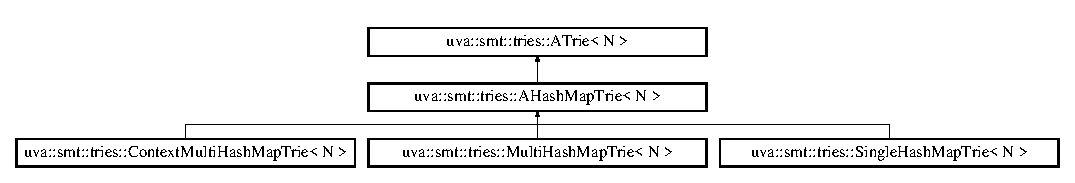
\includegraphics[height=0.788732cm]{classuva_1_1smt_1_1tries_1_1_a_trie}
\end{center}
\end{figure}
\subsection*{Public Member Functions}
\begin{DoxyCompactItemize}
\item 
\hyperlink{classuva_1_1smt_1_1tries_1_1_a_trie_adedfb4755e267882e91d9e0db499a1b7}{A\+Trie} (\hyperlink{classuva_1_1smt_1_1tries_1_1dictionary_1_1_a_word_index}{A\+Word\+Index} $\ast$\+\_\+p\+Word\+Index, bool is\+\_\+birmap\+\_\+hash\+\_\+cache=false)
\item 
virtual void \hyperlink{classuva_1_1smt_1_1tries_1_1_a_trie_a4c523028bdf0949d762d1bbfd3fdc262}{pre\+\_\+allocate} (const size\+\_\+t counts\mbox{[}N\mbox{]})
\item 
void \hyperlink{classuva_1_1smt_1_1tries_1_1_a_trie_afe3c10a349785d0401a93de1f46ecb11}{register\+\_\+m\+\_\+gram\+\_\+cache} (const \hyperlink{structuva_1_1smt_1_1tries_1_1mgrams_1_1_t___m___gram}{T\+\_\+\+M\+\_\+\+Gram} \&gram)
\item 
virtual void \hyperlink{classuva_1_1smt_1_1tries_1_1_a_trie_a3ff08588c72cd70dfc3d8129968d57b5}{add\+\_\+1\+\_\+gram} (const \hyperlink{structuva_1_1smt_1_1tries_1_1mgrams_1_1_t___m___gram}{T\+\_\+\+M\+\_\+\+Gram} \&gram)=0
\item 
virtual void \hyperlink{classuva_1_1smt_1_1tries_1_1_a_trie_a469f894057a536141d84be00e8bd8f5f}{add\+\_\+m\+\_\+gram} (const \hyperlink{structuva_1_1smt_1_1tries_1_1mgrams_1_1_t___m___gram}{T\+\_\+\+M\+\_\+\+Gram} \&gram)=0
\item 
virtual void \hyperlink{classuva_1_1smt_1_1tries_1_1_a_trie_aa4598e59915c77e7bf92d744d7d35f02}{add\+\_\+n\+\_\+gram} (const \hyperlink{structuva_1_1smt_1_1tries_1_1mgrams_1_1_t___m___gram}{T\+\_\+\+M\+\_\+\+Gram} \&gram)=0
\item 
virtual bool \hyperlink{classuva_1_1smt_1_1tries_1_1_a_trie_abaa5760dcdd087e3f977eae925862043}{is\+\_\+post\+\_\+grams} (const \hyperlink{namespaceuva_1_1smt_1_1tries_a20577a44b3a42d26524250634379b7cb}{T\+Model\+Level} level)
\item 
void \hyperlink{classuva_1_1smt_1_1tries_1_1_a_trie_a4416bd9ebf793e9d0d0a8ec715d0a3ce}{post\+\_\+grams} (const \hyperlink{namespaceuva_1_1smt_1_1tries_a20577a44b3a42d26524250634379b7cb}{T\+Model\+Level} level)
\item 
\hyperlink{namespaceuva_1_1smt_1_1tries_a20577a44b3a42d26524250634379b7cb}{T\+Model\+Level} \hyperlink{classuva_1_1smt_1_1tries_1_1_a_trie_a192510a887555617e703d03c145bbee5}{get\+\_\+max\+\_\+level} () const 
\item 
void \hyperlink{classuva_1_1smt_1_1tries_1_1_a_trie_a931c433a086f8f03dd6260e0d27dfd79}{query} (const \hyperlink{structuva_1_1smt_1_1tries_1_1mgrams_1_1_t___m___gram}{T\+\_\+\+M\+\_\+\+Gram} \&m\+\_\+gram, \hyperlink{structuva_1_1smt_1_1tries_1_1_t_query_result}{T\+Query\+Result} \&result)
\item 
\hyperlink{classuva_1_1smt_1_1tries_1_1dictionary_1_1_a_word_index}{A\+Word\+Index} $\ast$ \hyperlink{classuva_1_1smt_1_1tries_1_1_a_trie_a6d435385f750ffc9c129d1e800491ff8}{get\+\_\+word\+\_\+index} ()
\item 
virtual \hyperlink{classuva_1_1smt_1_1tries_1_1_a_trie_a5e72747b386ce5a2c9a41064c77e16e6}{$\sim$\+A\+Trie} ()
\item 
virtual void \hyperlink{classuva_1_1smt_1_1tries_1_1_a_trie_a4266759644e0ebfda77ab1a851a660af}{log\+\_\+trie\+\_\+type\+\_\+usage\+\_\+info} ()=0
\end{DoxyCompactItemize}
\subsection*{Static Public Attributes}
\begin{DoxyCompactItemize}
\item 
static const \hyperlink{namespaceuva_1_1smt_1_1tries_a20577a44b3a42d26524250634379b7cb}{T\+Model\+Level} \hyperlink{classuva_1_1smt_1_1tries_1_1_a_trie_af0f7dbcf0e0685c7acf49fd71710d138}{M\+G\+R\+A\+M\+\_\+\+I\+D\+X\+\_\+\+O\+F\+F\+S\+E\+T} = 2
\item 
static const \hyperlink{namespaceuva_1_1smt_1_1tries_a20577a44b3a42d26524250634379b7cb}{T\+Model\+Level} \hyperlink{classuva_1_1smt_1_1tries_1_1_a_trie_a24132c9483caf8dba629feaed57f61cd}{N\+U\+M\+\_\+\+M\+\_\+\+G\+R\+A\+M\+\_\+\+L\+E\+V\+E\+L\+S} = N -\/ \hyperlink{classuva_1_1smt_1_1tries_1_1_a_trie_af0f7dbcf0e0685c7acf49fd71710d138}{M\+G\+R\+A\+M\+\_\+\+I\+D\+X\+\_\+\+O\+F\+F\+S\+E\+T}
\item 
static const \hyperlink{namespaceuva_1_1smt_1_1tries_a20577a44b3a42d26524250634379b7cb}{T\+Model\+Level} \hyperlink{classuva_1_1smt_1_1tries_1_1_a_trie_a79334a0fd7b506705033a5bbc2041186}{N\+U\+M\+\_\+\+M\+\_\+\+N\+\_\+\+G\+R\+A\+M\+\_\+\+L\+E\+V\+E\+L\+S} = N -\/ 1
\item 
static const \hyperlink{namespaceuva_1_1smt_1_1tries_a20577a44b3a42d26524250634379b7cb}{T\+Model\+Level} \hyperlink{classuva_1_1smt_1_1tries_1_1_a_trie_ab3fc31d42c7407059bf2b242d424dc7b}{N\+\_\+\+G\+R\+A\+M\+\_\+\+I\+D\+X\+\_\+\+I\+N\+\_\+\+M\+\_\+\+N\+\_\+\+A\+R\+R} = N -\/ \hyperlink{classuva_1_1smt_1_1tries_1_1_a_trie_af0f7dbcf0e0685c7acf49fd71710d138}{M\+G\+R\+A\+M\+\_\+\+I\+D\+X\+\_\+\+O\+F\+F\+S\+E\+T}
\item 
static const \hyperlink{namespaceuva_1_1smt_1_1hashing_adcf22e1982ad09d3a63494c006267469}{T\+Short\+Id} \hyperlink{classuva_1_1smt_1_1tries_1_1_a_trie_aac34cbc190b3d5a2d32720a189fe8e72}{U\+N\+D\+E\+F\+I\+N\+E\+D\+\_\+\+A\+R\+R\+\_\+\+I\+D\+X} = 0
\item 
static const \hyperlink{namespaceuva_1_1smt_1_1hashing_adcf22e1982ad09d3a63494c006267469}{T\+Short\+Id} \hyperlink{classuva_1_1smt_1_1tries_1_1_a_trie_a364b68d11ca94eb1b38d78035376da39}{F\+I\+R\+S\+T\+\_\+\+V\+A\+L\+I\+D\+\_\+\+C\+T\+X\+\_\+\+I\+D} = \hyperlink{classuva_1_1smt_1_1tries_1_1_a_trie_aac34cbc190b3d5a2d32720a189fe8e72}{U\+N\+D\+E\+F\+I\+N\+E\+D\+\_\+\+A\+R\+R\+\_\+\+I\+D\+X} + 1
\end{DoxyCompactItemize}
\subsection*{Protected Member Functions}
\begin{DoxyCompactItemize}
\item 
const \hyperlink{namespaceuva_1_1smt_1_1hashing_adcf22e1982ad09d3a63494c006267469}{T\+Short\+Id} \& \hyperlink{classuva_1_1smt_1_1tries_1_1_a_trie_a3602c8aac334ee6ad76ceed1451d9da9}{get\+\_\+back\+\_\+off\+\_\+end\+\_\+word\+\_\+id} ()
\item 
const \hyperlink{namespaceuva_1_1smt_1_1hashing_adcf22e1982ad09d3a63494c006267469}{T\+Short\+Id} \& \hyperlink{classuva_1_1smt_1_1tries_1_1_a_trie_aebeb72b44be98d1bbe68e65c89ed9422}{get\+\_\+end\+\_\+word\+\_\+id} ()
\item 
void \hyperlink{classuva_1_1smt_1_1tries_1_1_a_trie_a2e9f9d3c04252a42349ea5b3bc526c61}{store\+\_\+m\+\_\+gram\+\_\+word\+\_\+ids} (const \hyperlink{structuva_1_1smt_1_1tries_1_1mgrams_1_1_t___m___gram}{T\+\_\+\+M\+\_\+\+Gram} \&m\+\_\+gram)
\item 
virtual void \hyperlink{classuva_1_1smt_1_1tries_1_1_a_trie_a5bc438e9f7c19bd18a8664527dcec9fb}{post\+\_\+1\+\_\+grams} ()
\item 
virtual void \hyperlink{classuva_1_1smt_1_1tries_1_1_a_trie_ae2ccab11c90970e5f6d5e84e0caa5256}{post\+\_\+m\+\_\+grams} (const \hyperlink{namespaceuva_1_1smt_1_1tries_a20577a44b3a42d26524250634379b7cb}{T\+Model\+Level} level)
\item 
virtual void \hyperlink{classuva_1_1smt_1_1tries_1_1_a_trie_a2e5175e70722e777d00cd38460dc465b}{post\+\_\+n\+\_\+grams} ()
\item 
bool \hyperlink{classuva_1_1smt_1_1tries_1_1_a_trie_aa56ac40acab11016dd544942c94b4bf8}{cache\+\_\+check\+\_\+add\+\_\+prob\+\_\+weight} (const \hyperlink{namespaceuva_1_1smt_1_1tries_a20577a44b3a42d26524250634379b7cb}{T\+Model\+Level} level, \hyperlink{namespaceuva_1_1smt_1_1tries_acd0660255dd9ef5d644f01de49102750}{T\+Log\+Prob\+Back\+Off} \&prob)
\item 
void \hyperlink{classuva_1_1smt_1_1tries_1_1_a_trie_a2c849f75181035f2e247612d410acbd3}{cache\+\_\+check\+\_\+add\+\_\+back\+\_\+off\+\_\+weight} (const \hyperlink{namespaceuva_1_1smt_1_1tries_a20577a44b3a42d26524250634379b7cb}{T\+Model\+Level} level, \hyperlink{namespaceuva_1_1smt_1_1tries_acd0660255dd9ef5d644f01de49102750}{T\+Log\+Prob\+Back\+Off} \&prob)
\item 
virtual bool \hyperlink{classuva_1_1smt_1_1tries_1_1_a_trie_ac6bb33e835e42c2b4c36b6d71f1d936c}{add\+\_\+prob\+\_\+weight} (const \hyperlink{namespaceuva_1_1smt_1_1tries_a20577a44b3a42d26524250634379b7cb}{T\+Model\+Level} level, \hyperlink{namespaceuva_1_1smt_1_1tries_acd0660255dd9ef5d644f01de49102750}{T\+Log\+Prob\+Back\+Off} \&prob)=0
\item 
virtual void \hyperlink{classuva_1_1smt_1_1tries_1_1_a_trie_aac350b954d22273e09db4890d80720e2}{add\+\_\+back\+\_\+off\+\_\+weight} (const \hyperlink{namespaceuva_1_1smt_1_1tries_a20577a44b3a42d26524250634379b7cb}{T\+Model\+Level} level, \hyperlink{namespaceuva_1_1smt_1_1tries_acd0660255dd9ef5d644f01de49102750}{T\+Log\+Prob\+Back\+Off} \&prob)=0
\end{DoxyCompactItemize}
\subsection*{Protected Attributes}
\begin{DoxyCompactItemize}
\item 
\hyperlink{classuva_1_1smt_1_1tries_1_1dictionary_1_1_a_word_index}{A\+Word\+Index} $\ast$ \hyperlink{classuva_1_1smt_1_1tries_1_1_a_trie_abc1f0fe671fcbc898b644715580a6b4a}{m\+\_\+word\+\_\+index\+\_\+ptr}
\item 
\hyperlink{namespaceuva_1_1smt_1_1hashing_adcf22e1982ad09d3a63494c006267469}{T\+Short\+Id} \hyperlink{classuva_1_1smt_1_1tries_1_1_a_trie_a8d2de9b0b513f6910f3e7bfeb24bd6a1}{m\+\_\+tmp\+\_\+word\+\_\+ids} \mbox{[}N\mbox{]}
\item 
const \hyperlink{structuva_1_1smt_1_1tries_1_1mgrams_1_1_t___m___gram}{T\+\_\+\+M\+\_\+\+Gram} $\ast$ \hyperlink{classuva_1_1smt_1_1tries_1_1_a_trie_a737d0794ed253550b080c58381176061}{m\+\_\+query\+\_\+ptr}
\item 
const bool \hyperlink{classuva_1_1smt_1_1tries_1_1_a_trie_ad34967837b387ce38390630fb5c28253}{m\+\_\+is\+\_\+birmap\+\_\+hash\+\_\+cache}
\end{DoxyCompactItemize}


\subsection{Detailed Description}
\subsubsection*{template$<$T\+Model\+Level N$>$class uva\+::smt\+::tries\+::\+A\+Trie$<$ N $>$}

This is a common abstract class for a Trie implementation. The purpose of having this as a template class is performance optimization. 
\begin{DoxyParams}{Parameters}
{\em N} & -\/ the maximum level of the considered N-\/gram, i.\+e. the N value \\
\hline
\end{DoxyParams}


\subsection{Constructor \& Destructor Documentation}
\hypertarget{classuva_1_1smt_1_1tries_1_1_a_trie_adedfb4755e267882e91d9e0db499a1b7}{}\index{uva\+::smt\+::tries\+::\+A\+Trie@{uva\+::smt\+::tries\+::\+A\+Trie}!A\+Trie@{A\+Trie}}
\index{A\+Trie@{A\+Trie}!uva\+::smt\+::tries\+::\+A\+Trie@{uva\+::smt\+::tries\+::\+A\+Trie}}
\subsubsection[{A\+Trie(\+A\+Word\+Index $\ast$\+\_\+p\+Word\+Index, bool is\+\_\+birmap\+\_\+hash\+\_\+cache=false)}]{\setlength{\rightskip}{0pt plus 5cm}template$<$T\+Model\+Level N$>$ {\bf uva\+::smt\+::tries\+::\+A\+Trie}$<$ N $>$\+::{\bf A\+Trie} (
\begin{DoxyParamCaption}
\item[{{\bf A\+Word\+Index} $\ast$}]{\+\_\+p\+Word\+Index, }
\item[{bool}]{is\+\_\+birmap\+\_\+hash\+\_\+cache = {\ttfamily false}}
\end{DoxyParamCaption}
)\hspace{0.3cm}{\ttfamily [inline]}, {\ttfamily [explicit]}}\label{classuva_1_1smt_1_1tries_1_1_a_trie_adedfb4755e267882e91d9e0db499a1b7}
The basic constructor 
\begin{DoxyParams}{Parameters}
{\em \+\_\+word\+Index} & the word index to be used \\
\hline
{\em is\+\_\+birmap\+\_\+hash\+\_\+cache} & -\/ allows to enable the bitmap hash cache for the M-\/grams. the latter records the hashes of all the M-\/gram present in the tries and then before querying checks if the hash of the queries M-\/gram is present if not then we do an immediate back-\/off, otherwise we search for the M-\/gram. This is an experimental feature therefore it the parameter\textquotesingle{}s default is false. Also this feature is to be used with the multi-\/level context index tries which require a lot of searching when looking for an M-\/gram. \\
\hline
\end{DoxyParams}
\hypertarget{classuva_1_1smt_1_1tries_1_1_a_trie_a5e72747b386ce5a2c9a41064c77e16e6}{}\index{uva\+::smt\+::tries\+::\+A\+Trie@{uva\+::smt\+::tries\+::\+A\+Trie}!````~A\+Trie@{$\sim$\+A\+Trie}}
\index{````~A\+Trie@{$\sim$\+A\+Trie}!uva\+::smt\+::tries\+::\+A\+Trie@{uva\+::smt\+::tries\+::\+A\+Trie}}
\subsubsection[{$\sim$\+A\+Trie()}]{\setlength{\rightskip}{0pt plus 5cm}template$<$T\+Model\+Level N$>$ virtual {\bf uva\+::smt\+::tries\+::\+A\+Trie}$<$ N $>$\+::$\sim${\bf A\+Trie} (
\begin{DoxyParamCaption}
{}
\end{DoxyParamCaption}
)\hspace{0.3cm}{\ttfamily [inline]}, {\ttfamily [virtual]}}\label{classuva_1_1smt_1_1tries_1_1_a_trie_a5e72747b386ce5a2c9a41064c77e16e6}
The basic class destructor 

\subsection{Member Function Documentation}
\hypertarget{classuva_1_1smt_1_1tries_1_1_a_trie_a3ff08588c72cd70dfc3d8129968d57b5}{}\index{uva\+::smt\+::tries\+::\+A\+Trie@{uva\+::smt\+::tries\+::\+A\+Trie}!add\+\_\+1\+\_\+gram@{add\+\_\+1\+\_\+gram}}
\index{add\+\_\+1\+\_\+gram@{add\+\_\+1\+\_\+gram}!uva\+::smt\+::tries\+::\+A\+Trie@{uva\+::smt\+::tries\+::\+A\+Trie}}
\subsubsection[{add\+\_\+1\+\_\+gram(const T\+\_\+\+M\+\_\+\+Gram \&gram)=0}]{\setlength{\rightskip}{0pt plus 5cm}template$<$T\+Model\+Level N$>$ virtual void {\bf uva\+::smt\+::tries\+::\+A\+Trie}$<$ N $>$\+::add\+\_\+1\+\_\+gram (
\begin{DoxyParamCaption}
\item[{const {\bf T\+\_\+\+M\+\_\+\+Gram} \&}]{gram}
\end{DoxyParamCaption}
)\hspace{0.3cm}{\ttfamily [pure virtual]}}\label{classuva_1_1smt_1_1tries_1_1_a_trie_a3ff08588c72cd70dfc3d8129968d57b5}
This method adds a 1-\/\+Gram (word) to the trie. It it snot guaranteed that the parameter will be checked to be a 1-\/\+Gram! 
\begin{DoxyParams}{Parameters}
{\em gram} & the 1-\/\+Gram data \\
\hline
\end{DoxyParams}


Implemented in \hyperlink{classuva_1_1smt_1_1tries_1_1_g2_d_map_trie_a54e165e0783f90a74f3bb9675c012a28}{uva\+::smt\+::tries\+::\+G2\+D\+Map\+Trie$<$ N $>$}, and \hyperlink{classuva_1_1smt_1_1tries_1_1_a_layered_trie_a36a55b5d2d85c9b8de4f8915956df4b5}{uva\+::smt\+::tries\+::\+A\+Layered\+Trie$<$ N $>$}.

\hypertarget{classuva_1_1smt_1_1tries_1_1_a_trie_aac350b954d22273e09db4890d80720e2}{}\index{uva\+::smt\+::tries\+::\+A\+Trie@{uva\+::smt\+::tries\+::\+A\+Trie}!add\+\_\+back\+\_\+off\+\_\+weight@{add\+\_\+back\+\_\+off\+\_\+weight}}
\index{add\+\_\+back\+\_\+off\+\_\+weight@{add\+\_\+back\+\_\+off\+\_\+weight}!uva\+::smt\+::tries\+::\+A\+Trie@{uva\+::smt\+::tries\+::\+A\+Trie}}
\subsubsection[{add\+\_\+back\+\_\+off\+\_\+weight(const T\+Model\+Level level, T\+Log\+Prob\+Back\+Off \&prob)=0}]{\setlength{\rightskip}{0pt plus 5cm}template$<$T\+Model\+Level N$>$ virtual void {\bf uva\+::smt\+::tries\+::\+A\+Trie}$<$ N $>$\+::add\+\_\+back\+\_\+off\+\_\+weight (
\begin{DoxyParamCaption}
\item[{const {\bf T\+Model\+Level}}]{level, }
\item[{{\bf T\+Log\+Prob\+Back\+Off} \&}]{prob}
\end{DoxyParamCaption}
)\hspace{0.3cm}{\ttfamily [protected]}, {\ttfamily [pure virtual]}}\label{classuva_1_1smt_1_1tries_1_1_a_trie_aac350b954d22273e09db4890d80720e2}
This function allows to retrieve the back-\/off stored for the given M-\/gram level. If the value is found then it must be added to the prob parameter of the function. If the value is not found then the prob parameter of the function must not be changed. In that case the back-\/off weight is just zero. 
\begin{DoxyParams}{Parameters}
{\em level} & the level of the M-\/gram we need to compute probability for. \\
\hline
{\em prob} & the probability variable that is to be increased with the found back-\/off weight \\
\hline
\end{DoxyParams}


Implemented in \hyperlink{classuva_1_1smt_1_1tries_1_1_a_layered_trie_a3cd19ce2041e3538ca7628105db1acec}{uva\+::smt\+::tries\+::\+A\+Layered\+Trie$<$ N $>$}, and \hyperlink{classuva_1_1smt_1_1tries_1_1_g2_d_map_trie_a48646b91ccd38fcd89969ae5fd39a324}{uva\+::smt\+::tries\+::\+G2\+D\+Map\+Trie$<$ N $>$}.

\hypertarget{classuva_1_1smt_1_1tries_1_1_a_trie_a469f894057a536141d84be00e8bd8f5f}{}\index{uva\+::smt\+::tries\+::\+A\+Trie@{uva\+::smt\+::tries\+::\+A\+Trie}!add\+\_\+m\+\_\+gram@{add\+\_\+m\+\_\+gram}}
\index{add\+\_\+m\+\_\+gram@{add\+\_\+m\+\_\+gram}!uva\+::smt\+::tries\+::\+A\+Trie@{uva\+::smt\+::tries\+::\+A\+Trie}}
\subsubsection[{add\+\_\+m\+\_\+gram(const T\+\_\+\+M\+\_\+\+Gram \&gram)=0}]{\setlength{\rightskip}{0pt plus 5cm}template$<$T\+Model\+Level N$>$ virtual void {\bf uva\+::smt\+::tries\+::\+A\+Trie}$<$ N $>$\+::add\+\_\+m\+\_\+gram (
\begin{DoxyParamCaption}
\item[{const {\bf T\+\_\+\+M\+\_\+\+Gram} \&}]{gram}
\end{DoxyParamCaption}
)\hspace{0.3cm}{\ttfamily [pure virtual]}}\label{classuva_1_1smt_1_1tries_1_1_a_trie_a469f894057a536141d84be00e8bd8f5f}
This method adds a M-\/\+Gram (word) to the trie where 1 $<$ M $<$ N 
\begin{DoxyParams}{Parameters}
{\em gram} & the M-\/\+Gram data \\
\hline
\end{DoxyParams}

\begin{DoxyExceptions}{Exceptions}
{\em Exception} & if the level of this M-\/gram is not such that 1 $<$ M $<$ N \\
\hline
\end{DoxyExceptions}


Implemented in \hyperlink{classuva_1_1smt_1_1tries_1_1_g2_d_map_trie_a4df6000a2413384cb895d70455fb085a}{uva\+::smt\+::tries\+::\+G2\+D\+Map\+Trie$<$ N $>$}, and \hyperlink{classuva_1_1smt_1_1tries_1_1_a_layered_trie_aed865ddfcfddb0f924d7424f9c2dba30}{uva\+::smt\+::tries\+::\+A\+Layered\+Trie$<$ N $>$}.

\hypertarget{classuva_1_1smt_1_1tries_1_1_a_trie_aa4598e59915c77e7bf92d744d7d35f02}{}\index{uva\+::smt\+::tries\+::\+A\+Trie@{uva\+::smt\+::tries\+::\+A\+Trie}!add\+\_\+n\+\_\+gram@{add\+\_\+n\+\_\+gram}}
\index{add\+\_\+n\+\_\+gram@{add\+\_\+n\+\_\+gram}!uva\+::smt\+::tries\+::\+A\+Trie@{uva\+::smt\+::tries\+::\+A\+Trie}}
\subsubsection[{add\+\_\+n\+\_\+gram(const T\+\_\+\+M\+\_\+\+Gram \&gram)=0}]{\setlength{\rightskip}{0pt plus 5cm}template$<$T\+Model\+Level N$>$ virtual void {\bf uva\+::smt\+::tries\+::\+A\+Trie}$<$ N $>$\+::add\+\_\+n\+\_\+gram (
\begin{DoxyParamCaption}
\item[{const {\bf T\+\_\+\+M\+\_\+\+Gram} \&}]{gram}
\end{DoxyParamCaption}
)\hspace{0.3cm}{\ttfamily [pure virtual]}}\label{classuva_1_1smt_1_1tries_1_1_a_trie_aa4598e59915c77e7bf92d744d7d35f02}
This method adds a N-\/\+Gram (word) to the trie where It it snot guaranteed that the parameter will be checked to be a N-\/\+Gram! 
\begin{DoxyParams}{Parameters}
{\em gram} & the N-\/\+Gram data \\
\hline
\end{DoxyParams}


Implemented in \hyperlink{classuva_1_1smt_1_1tries_1_1_g2_d_map_trie_a0b9497cafbcd2d5330b76ea2ae5d8e87}{uva\+::smt\+::tries\+::\+G2\+D\+Map\+Trie$<$ N $>$}, and \hyperlink{classuva_1_1smt_1_1tries_1_1_a_layered_trie_a4640ef130893289b79b357bd840d1d49}{uva\+::smt\+::tries\+::\+A\+Layered\+Trie$<$ N $>$}.

\hypertarget{classuva_1_1smt_1_1tries_1_1_a_trie_ac6bb33e835e42c2b4c36b6d71f1d936c}{}\index{uva\+::smt\+::tries\+::\+A\+Trie@{uva\+::smt\+::tries\+::\+A\+Trie}!add\+\_\+prob\+\_\+weight@{add\+\_\+prob\+\_\+weight}}
\index{add\+\_\+prob\+\_\+weight@{add\+\_\+prob\+\_\+weight}!uva\+::smt\+::tries\+::\+A\+Trie@{uva\+::smt\+::tries\+::\+A\+Trie}}
\subsubsection[{add\+\_\+prob\+\_\+weight(const T\+Model\+Level level, T\+Log\+Prob\+Back\+Off \&prob)=0}]{\setlength{\rightskip}{0pt plus 5cm}template$<$T\+Model\+Level N$>$ virtual bool {\bf uva\+::smt\+::tries\+::\+A\+Trie}$<$ N $>$\+::add\+\_\+prob\+\_\+weight (
\begin{DoxyParamCaption}
\item[{const {\bf T\+Model\+Level}}]{level, }
\item[{{\bf T\+Log\+Prob\+Back\+Off} \&}]{prob}
\end{DoxyParamCaption}
)\hspace{0.3cm}{\ttfamily [protected]}, {\ttfamily [pure virtual]}}\label{classuva_1_1smt_1_1tries_1_1_a_trie_ac6bb33e835e42c2b4c36b6d71f1d936c}
This function allows to retrieve the probability stored for the given M-\/gram level. If the value is found then it must be added to the prob parameter of the function. If the value is not found then the prob parameter of the function must not be changed. 
\begin{DoxyParams}{Parameters}
{\em level} & the level of the M-\/gram we need to compute probability for. \\
\hline
{\em prob} & the probability variable that is to be increased with the found probability weight \\
\hline
\end{DoxyParams}
\begin{DoxyReturn}{Returns}
true if the probability for the given M-\/gram level could be found, otherwise false. 
\end{DoxyReturn}


Implemented in \hyperlink{classuva_1_1smt_1_1tries_1_1_a_layered_trie_a715fbbe90bbb52d7f86532748ca53d39}{uva\+::smt\+::tries\+::\+A\+Layered\+Trie$<$ N $>$}, and \hyperlink{classuva_1_1smt_1_1tries_1_1_g2_d_map_trie_a116303b3bc78d4df59e1ed09d2270708}{uva\+::smt\+::tries\+::\+G2\+D\+Map\+Trie$<$ N $>$}.

\hypertarget{classuva_1_1smt_1_1tries_1_1_a_trie_a2c849f75181035f2e247612d410acbd3}{}\index{uva\+::smt\+::tries\+::\+A\+Trie@{uva\+::smt\+::tries\+::\+A\+Trie}!cache\+\_\+check\+\_\+add\+\_\+back\+\_\+off\+\_\+weight@{cache\+\_\+check\+\_\+add\+\_\+back\+\_\+off\+\_\+weight}}
\index{cache\+\_\+check\+\_\+add\+\_\+back\+\_\+off\+\_\+weight@{cache\+\_\+check\+\_\+add\+\_\+back\+\_\+off\+\_\+weight}!uva\+::smt\+::tries\+::\+A\+Trie@{uva\+::smt\+::tries\+::\+A\+Trie}}
\subsubsection[{cache\+\_\+check\+\_\+add\+\_\+back\+\_\+off\+\_\+weight(const T\+Model\+Level level, T\+Log\+Prob\+Back\+Off \&prob)}]{\setlength{\rightskip}{0pt plus 5cm}template$<$T\+Model\+Level N$>$ void {\bf uva\+::smt\+::tries\+::\+A\+Trie}$<$ N $>$\+::cache\+\_\+check\+\_\+add\+\_\+back\+\_\+off\+\_\+weight (
\begin{DoxyParamCaption}
\item[{const {\bf T\+Model\+Level}}]{level, }
\item[{{\bf T\+Log\+Prob\+Back\+Off} \&}]{prob}
\end{DoxyParamCaption}
)\hspace{0.3cm}{\ttfamily [inline]}, {\ttfamily [protected]}}\label{classuva_1_1smt_1_1tries_1_1_a_trie_a2c849f75181035f2e247612d410acbd3}
Allows to get the back-\/off weight value also by checking the cache. If the back-\/off is not found then the probability value is to stay intact. Then the back-\/off weight is considered to be zero! 
\begin{DoxyParams}{Parameters}
{\em level} & the M-\/gram level to get the back-\/off weight for \\
\hline
{\em prob} & the probability to be added by the found back-\/off weight \\
\hline
\end{DoxyParams}
\hypertarget{classuva_1_1smt_1_1tries_1_1_a_trie_aa56ac40acab11016dd544942c94b4bf8}{}\index{uva\+::smt\+::tries\+::\+A\+Trie@{uva\+::smt\+::tries\+::\+A\+Trie}!cache\+\_\+check\+\_\+add\+\_\+prob\+\_\+weight@{cache\+\_\+check\+\_\+add\+\_\+prob\+\_\+weight}}
\index{cache\+\_\+check\+\_\+add\+\_\+prob\+\_\+weight@{cache\+\_\+check\+\_\+add\+\_\+prob\+\_\+weight}!uva\+::smt\+::tries\+::\+A\+Trie@{uva\+::smt\+::tries\+::\+A\+Trie}}
\subsubsection[{cache\+\_\+check\+\_\+add\+\_\+prob\+\_\+weight(const T\+Model\+Level level, T\+Log\+Prob\+Back\+Off \&prob)}]{\setlength{\rightskip}{0pt plus 5cm}template$<$T\+Model\+Level N$>$ bool {\bf uva\+::smt\+::tries\+::\+A\+Trie}$<$ N $>$\+::cache\+\_\+check\+\_\+add\+\_\+prob\+\_\+weight (
\begin{DoxyParamCaption}
\item[{const {\bf T\+Model\+Level}}]{level, }
\item[{{\bf T\+Log\+Prob\+Back\+Off} \&}]{prob}
\end{DoxyParamCaption}
)\hspace{0.3cm}{\ttfamily [inline]}, {\ttfamily [protected]}}\label{classuva_1_1smt_1_1tries_1_1_a_trie_aa56ac40acab11016dd544942c94b4bf8}
Allows to get the probability value also by checking the cache. If the probability is not found then the prob value is to stay intact! 
\begin{DoxyParams}{Parameters}
{\em level} & the M-\/gram level to get the probability for \\
\hline
{\em prob} & the probability to be filled in \\
\hline
\end{DoxyParams}
\begin{DoxyReturn}{Returns}
true if the probability has been found, otherwise false 
\end{DoxyReturn}
\hypertarget{classuva_1_1smt_1_1tries_1_1_a_trie_a3602c8aac334ee6ad76ceed1451d9da9}{}\index{uva\+::smt\+::tries\+::\+A\+Trie@{uva\+::smt\+::tries\+::\+A\+Trie}!get\+\_\+back\+\_\+off\+\_\+end\+\_\+word\+\_\+id@{get\+\_\+back\+\_\+off\+\_\+end\+\_\+word\+\_\+id}}
\index{get\+\_\+back\+\_\+off\+\_\+end\+\_\+word\+\_\+id@{get\+\_\+back\+\_\+off\+\_\+end\+\_\+word\+\_\+id}!uva\+::smt\+::tries\+::\+A\+Trie@{uva\+::smt\+::tries\+::\+A\+Trie}}
\subsubsection[{get\+\_\+back\+\_\+off\+\_\+end\+\_\+word\+\_\+id()}]{\setlength{\rightskip}{0pt plus 5cm}template$<$T\+Model\+Level N$>$ const {\bf T\+Short\+Id}\& {\bf uva\+::smt\+::tries\+::\+A\+Trie}$<$ N $>$\+::get\+\_\+back\+\_\+off\+\_\+end\+\_\+word\+\_\+id (
\begin{DoxyParamCaption}
{}
\end{DoxyParamCaption}
)\hspace{0.3cm}{\ttfamily [inline]}, {\ttfamily [protected]}}\label{classuva_1_1smt_1_1tries_1_1_a_trie_a3602c8aac334ee6ad76ceed1451d9da9}
Gets the word hash for the end word of the back-\/off M-\/\+Gram \begin{DoxyReturn}{Returns}
the word hash for the end word of the back-\/off M-\/\+Gram 
\end{DoxyReturn}
\hypertarget{classuva_1_1smt_1_1tries_1_1_a_trie_aebeb72b44be98d1bbe68e65c89ed9422}{}\index{uva\+::smt\+::tries\+::\+A\+Trie@{uva\+::smt\+::tries\+::\+A\+Trie}!get\+\_\+end\+\_\+word\+\_\+id@{get\+\_\+end\+\_\+word\+\_\+id}}
\index{get\+\_\+end\+\_\+word\+\_\+id@{get\+\_\+end\+\_\+word\+\_\+id}!uva\+::smt\+::tries\+::\+A\+Trie@{uva\+::smt\+::tries\+::\+A\+Trie}}
\subsubsection[{get\+\_\+end\+\_\+word\+\_\+id()}]{\setlength{\rightskip}{0pt plus 5cm}template$<$T\+Model\+Level N$>$ const {\bf T\+Short\+Id}\& {\bf uva\+::smt\+::tries\+::\+A\+Trie}$<$ N $>$\+::get\+\_\+end\+\_\+word\+\_\+id (
\begin{DoxyParamCaption}
{}
\end{DoxyParamCaption}
)\hspace{0.3cm}{\ttfamily [inline]}, {\ttfamily [protected]}}\label{classuva_1_1smt_1_1tries_1_1_a_trie_aebeb72b44be98d1bbe68e65c89ed9422}
Gets the word hash for the last word in the M-\/gram \begin{DoxyReturn}{Returns}
the word hash for the last word in the M-\/gram 
\end{DoxyReturn}
\hypertarget{classuva_1_1smt_1_1tries_1_1_a_trie_a192510a887555617e703d03c145bbee5}{}\index{uva\+::smt\+::tries\+::\+A\+Trie@{uva\+::smt\+::tries\+::\+A\+Trie}!get\+\_\+max\+\_\+level@{get\+\_\+max\+\_\+level}}
\index{get\+\_\+max\+\_\+level@{get\+\_\+max\+\_\+level}!uva\+::smt\+::tries\+::\+A\+Trie@{uva\+::smt\+::tries\+::\+A\+Trie}}
\subsubsection[{get\+\_\+max\+\_\+level() const }]{\setlength{\rightskip}{0pt plus 5cm}template$<$T\+Model\+Level N$>$ {\bf T\+Model\+Level} {\bf uva\+::smt\+::tries\+::\+A\+Trie}$<$ N $>$\+::get\+\_\+max\+\_\+level (
\begin{DoxyParamCaption}
{}
\end{DoxyParamCaption}
) const\hspace{0.3cm}{\ttfamily [inline]}}\label{classuva_1_1smt_1_1tries_1_1_a_trie_a192510a887555617e703d03c145bbee5}
Returns the maximum length of the considered N-\/\+Grams \begin{DoxyReturn}{Returns}
the maximum length of the considered N-\/\+Grams 
\end{DoxyReturn}
\hypertarget{classuva_1_1smt_1_1tries_1_1_a_trie_a6d435385f750ffc9c129d1e800491ff8}{}\index{uva\+::smt\+::tries\+::\+A\+Trie@{uva\+::smt\+::tries\+::\+A\+Trie}!get\+\_\+word\+\_\+index@{get\+\_\+word\+\_\+index}}
\index{get\+\_\+word\+\_\+index@{get\+\_\+word\+\_\+index}!uva\+::smt\+::tries\+::\+A\+Trie@{uva\+::smt\+::tries\+::\+A\+Trie}}
\subsubsection[{get\+\_\+word\+\_\+index()}]{\setlength{\rightskip}{0pt plus 5cm}template$<$T\+Model\+Level N$>$ {\bf A\+Word\+Index}$\ast$ {\bf uva\+::smt\+::tries\+::\+A\+Trie}$<$ N $>$\+::get\+\_\+word\+\_\+index (
\begin{DoxyParamCaption}
{}
\end{DoxyParamCaption}
)\hspace{0.3cm}{\ttfamily [inline]}}\label{classuva_1_1smt_1_1tries_1_1_a_trie_a6d435385f750ffc9c129d1e800491ff8}
Allows to retrieve the stored word index, if any \begin{DoxyReturn}{Returns}
the pointer to the stored word index or N\+U\+L\+L if none 
\end{DoxyReturn}
\hypertarget{classuva_1_1smt_1_1tries_1_1_a_trie_abaa5760dcdd087e3f977eae925862043}{}\index{uva\+::smt\+::tries\+::\+A\+Trie@{uva\+::smt\+::tries\+::\+A\+Trie}!is\+\_\+post\+\_\+grams@{is\+\_\+post\+\_\+grams}}
\index{is\+\_\+post\+\_\+grams@{is\+\_\+post\+\_\+grams}!uva\+::smt\+::tries\+::\+A\+Trie@{uva\+::smt\+::tries\+::\+A\+Trie}}
\subsubsection[{is\+\_\+post\+\_\+grams(const T\+Model\+Level level)}]{\setlength{\rightskip}{0pt plus 5cm}template$<$T\+Model\+Level N$>$ virtual bool {\bf uva\+::smt\+::tries\+::\+A\+Trie}$<$ N $>$\+::is\+\_\+post\+\_\+grams (
\begin{DoxyParamCaption}
\item[{const {\bf T\+Model\+Level}}]{level}
\end{DoxyParamCaption}
)\hspace{0.3cm}{\ttfamily [inline]}, {\ttfamily [virtual]}}\label{classuva_1_1smt_1_1tries_1_1_a_trie_abaa5760dcdd087e3f977eae925862043}
This method allows to check if post processing should be called after all the X level grams are read. This method is virtual. 
\begin{DoxyParams}{Parameters}
{\em level} & the level of the X-\/grams that were finished to be read \\
\hline
\end{DoxyParams}


Reimplemented in \hyperlink{classuva_1_1smt_1_1tries_1_1_c2_w_array_trie_adc09a52f78098d1011fc481f36cf19f9}{uva\+::smt\+::tries\+::\+C2\+W\+Array\+Trie$<$ N $>$}, \hyperlink{classuva_1_1smt_1_1tries_1_1_w2_c_array_trie_a89ce79512b08afab4ece1158eff68fee}{uva\+::smt\+::tries\+::\+W2\+C\+Array\+Trie$<$ N $>$}, and \hyperlink{classuva_1_1smt_1_1tries_1_1_g2_d_map_trie_af24619edf2b59c3299a32838512bb6bb}{uva\+::smt\+::tries\+::\+G2\+D\+Map\+Trie$<$ N $>$}.

\hypertarget{classuva_1_1smt_1_1tries_1_1_a_trie_a4266759644e0ebfda77ab1a851a660af}{}\index{uva\+::smt\+::tries\+::\+A\+Trie@{uva\+::smt\+::tries\+::\+A\+Trie}!log\+\_\+trie\+\_\+type\+\_\+usage\+\_\+info@{log\+\_\+trie\+\_\+type\+\_\+usage\+\_\+info}}
\index{log\+\_\+trie\+\_\+type\+\_\+usage\+\_\+info@{log\+\_\+trie\+\_\+type\+\_\+usage\+\_\+info}!uva\+::smt\+::tries\+::\+A\+Trie@{uva\+::smt\+::tries\+::\+A\+Trie}}
\subsubsection[{log\+\_\+trie\+\_\+type\+\_\+usage\+\_\+info()=0}]{\setlength{\rightskip}{0pt plus 5cm}template$<$T\+Model\+Level N$>$ virtual void {\bf uva\+::smt\+::tries\+::\+A\+Trie}$<$ N $>$\+::log\+\_\+trie\+\_\+type\+\_\+usage\+\_\+info (
\begin{DoxyParamCaption}
{}
\end{DoxyParamCaption}
)\hspace{0.3cm}{\ttfamily [pure virtual]}}\label{classuva_1_1smt_1_1tries_1_1_a_trie_a4266759644e0ebfda77ab1a851a660af}
Allows to log the information about the instantiated trie type 

Implemented in \hyperlink{classuva_1_1smt_1_1tries_1_1_c2_w_array_trie_a29d456f70c6d4d9f6c6cda728a3c1b60}{uva\+::smt\+::tries\+::\+C2\+W\+Array\+Trie$<$ N $>$}, \hyperlink{classuva_1_1smt_1_1tries_1_1_c2_d_map_trie_aaba97e128f3129776ca46e75f5c005e1}{uva\+::smt\+::tries\+::\+C2\+D\+Map\+Trie$<$ N $>$}, \hyperlink{classuva_1_1smt_1_1tries_1_1_w2_c_array_trie_a2137d9c6ffd08ca95bea39c7604f9b13}{uva\+::smt\+::tries\+::\+W2\+C\+Array\+Trie$<$ N $>$}, \hyperlink{classuva_1_1smt_1_1tries_1_1_g2_d_map_trie_a8a5d0c8c65881a5895692b726f2f8321}{uva\+::smt\+::tries\+::\+G2\+D\+Map\+Trie$<$ N $>$}, \hyperlink{classuva_1_1smt_1_1tries_1_1_c2_d_hybrid_trie_aef676e4ee209417b74ee1a2965b99bb6}{uva\+::smt\+::tries\+::\+C2\+D\+Hybrid\+Trie$<$ N $>$}, and \hyperlink{classuva_1_1smt_1_1tries_1_1_w2_c_hybrid_trie_acfd9364a101a2ed142096fe91265d407}{uva\+::smt\+::tries\+::\+W2\+C\+Hybrid\+Trie$<$ N, Storage\+Factory, Storage\+Container $>$}.

\hypertarget{classuva_1_1smt_1_1tries_1_1_a_trie_a5bc438e9f7c19bd18a8664527dcec9fb}{}\index{uva\+::smt\+::tries\+::\+A\+Trie@{uva\+::smt\+::tries\+::\+A\+Trie}!post\+\_\+1\+\_\+grams@{post\+\_\+1\+\_\+grams}}
\index{post\+\_\+1\+\_\+grams@{post\+\_\+1\+\_\+grams}!uva\+::smt\+::tries\+::\+A\+Trie@{uva\+::smt\+::tries\+::\+A\+Trie}}
\subsubsection[{post\+\_\+1\+\_\+grams()}]{\setlength{\rightskip}{0pt plus 5cm}template$<$T\+Model\+Level N$>$ virtual void {\bf uva\+::smt\+::tries\+::\+A\+Trie}$<$ N $>$\+::post\+\_\+1\+\_\+grams (
\begin{DoxyParamCaption}
{}
\end{DoxyParamCaption}
)\hspace{0.3cm}{\ttfamily [inline]}, {\ttfamily [protected]}, {\ttfamily [virtual]}}\label{classuva_1_1smt_1_1tries_1_1_a_trie_a5bc438e9f7c19bd18a8664527dcec9fb}
This method will be called after all the 1-\/grams are read. The default implementation of this method is present. If overridden must be called from the child method. \hypertarget{classuva_1_1smt_1_1tries_1_1_a_trie_a4416bd9ebf793e9d0d0a8ec715d0a3ce}{}\index{uva\+::smt\+::tries\+::\+A\+Trie@{uva\+::smt\+::tries\+::\+A\+Trie}!post\+\_\+grams@{post\+\_\+grams}}
\index{post\+\_\+grams@{post\+\_\+grams}!uva\+::smt\+::tries\+::\+A\+Trie@{uva\+::smt\+::tries\+::\+A\+Trie}}
\subsubsection[{post\+\_\+grams(const T\+Model\+Level level)}]{\setlength{\rightskip}{0pt plus 5cm}template$<$T\+Model\+Level N$>$ void {\bf uva\+::smt\+::tries\+::\+A\+Trie}$<$ N $>$\+::post\+\_\+grams (
\begin{DoxyParamCaption}
\item[{const {\bf T\+Model\+Level}}]{level}
\end{DoxyParamCaption}
)\hspace{0.3cm}{\ttfamily [inline]}}\label{classuva_1_1smt_1_1tries_1_1_a_trie_a4416bd9ebf793e9d0d0a8ec715d0a3ce}
This method should be called after all the X level grams are read. 
\begin{DoxyParams}{Parameters}
{\em level} & the level of the X-\/grams that were finished to be read \\
\hline
\end{DoxyParams}
\hypertarget{classuva_1_1smt_1_1tries_1_1_a_trie_ae2ccab11c90970e5f6d5e84e0caa5256}{}\index{uva\+::smt\+::tries\+::\+A\+Trie@{uva\+::smt\+::tries\+::\+A\+Trie}!post\+\_\+m\+\_\+grams@{post\+\_\+m\+\_\+grams}}
\index{post\+\_\+m\+\_\+grams@{post\+\_\+m\+\_\+grams}!uva\+::smt\+::tries\+::\+A\+Trie@{uva\+::smt\+::tries\+::\+A\+Trie}}
\subsubsection[{post\+\_\+m\+\_\+grams(const T\+Model\+Level level)}]{\setlength{\rightskip}{0pt plus 5cm}template$<$T\+Model\+Level N$>$ virtual void {\bf uva\+::smt\+::tries\+::\+A\+Trie}$<$ N $>$\+::post\+\_\+m\+\_\+grams (
\begin{DoxyParamCaption}
\item[{const {\bf T\+Model\+Level}}]{level}
\end{DoxyParamCaption}
)\hspace{0.3cm}{\ttfamily [inline]}, {\ttfamily [protected]}, {\ttfamily [virtual]}}\label{classuva_1_1smt_1_1tries_1_1_a_trie_ae2ccab11c90970e5f6d5e84e0caa5256}
This method will be called after all the M-\/grams are read. The default implementation of this method is present. If overridden must be called from the child method. 
\begin{DoxyParams}{Parameters}
{\em level} & the level of the M-\/grams that were finished to be read \\
\hline
\end{DoxyParams}


Reimplemented in \hyperlink{classuva_1_1smt_1_1tries_1_1_c2_w_array_trie_a1a412c43dc00b64041cd4bb8245df1dd}{uva\+::smt\+::tries\+::\+C2\+W\+Array\+Trie$<$ N $>$}, \hyperlink{classuva_1_1smt_1_1tries_1_1_w2_c_array_trie_a0e9d011553a7d2a3651f6c9b48cc0c69}{uva\+::smt\+::tries\+::\+W2\+C\+Array\+Trie$<$ N $>$}, and \hyperlink{classuva_1_1smt_1_1tries_1_1_g2_d_map_trie_a593414c1e5fbd7522c6ef31643848532}{uva\+::smt\+::tries\+::\+G2\+D\+Map\+Trie$<$ N $>$}.

\hypertarget{classuva_1_1smt_1_1tries_1_1_a_trie_a2e5175e70722e777d00cd38460dc465b}{}\index{uva\+::smt\+::tries\+::\+A\+Trie@{uva\+::smt\+::tries\+::\+A\+Trie}!post\+\_\+n\+\_\+grams@{post\+\_\+n\+\_\+grams}}
\index{post\+\_\+n\+\_\+grams@{post\+\_\+n\+\_\+grams}!uva\+::smt\+::tries\+::\+A\+Trie@{uva\+::smt\+::tries\+::\+A\+Trie}}
\subsubsection[{post\+\_\+n\+\_\+grams()}]{\setlength{\rightskip}{0pt plus 5cm}template$<$T\+Model\+Level N$>$ virtual void {\bf uva\+::smt\+::tries\+::\+A\+Trie}$<$ N $>$\+::post\+\_\+n\+\_\+grams (
\begin{DoxyParamCaption}
{}
\end{DoxyParamCaption}
)\hspace{0.3cm}{\ttfamily [inline]}, {\ttfamily [protected]}, {\ttfamily [virtual]}}\label{classuva_1_1smt_1_1tries_1_1_a_trie_a2e5175e70722e777d00cd38460dc465b}
This method will be called after all the N-\/grams are read. The default implementation of this method is present. If overridden must be called from the child method. 

Reimplemented in \hyperlink{classuva_1_1smt_1_1tries_1_1_c2_w_array_trie_a0ceb69ca063fb5cadaf1d5903dd5ffbc}{uva\+::smt\+::tries\+::\+C2\+W\+Array\+Trie$<$ N $>$}, \hyperlink{classuva_1_1smt_1_1tries_1_1_w2_c_array_trie_aff8942ff3f4b91f4a79710635d2c637c}{uva\+::smt\+::tries\+::\+W2\+C\+Array\+Trie$<$ N $>$}, and \hyperlink{classuva_1_1smt_1_1tries_1_1_g2_d_map_trie_a3cb280a715f72c97aaaf4ce0f05e657a}{uva\+::smt\+::tries\+::\+G2\+D\+Map\+Trie$<$ N $>$}.

\hypertarget{classuva_1_1smt_1_1tries_1_1_a_trie_a4c523028bdf0949d762d1bbfd3fdc262}{}\index{uva\+::smt\+::tries\+::\+A\+Trie@{uva\+::smt\+::tries\+::\+A\+Trie}!pre\+\_\+allocate@{pre\+\_\+allocate}}
\index{pre\+\_\+allocate@{pre\+\_\+allocate}!uva\+::smt\+::tries\+::\+A\+Trie@{uva\+::smt\+::tries\+::\+A\+Trie}}
\subsubsection[{pre\+\_\+allocate(const size\+\_\+t counts[N])}]{\setlength{\rightskip}{0pt plus 5cm}template$<$T\+Model\+Level N$>$ virtual void {\bf uva\+::smt\+::tries\+::\+A\+Trie}$<$ N $>$\+::pre\+\_\+allocate (
\begin{DoxyParamCaption}
\item[{const size\+\_\+t}]{counts\mbox{[}\+N\mbox{]}}
\end{DoxyParamCaption}
)\hspace{0.3cm}{\ttfamily [inline]}, {\ttfamily [virtual]}}\label{classuva_1_1smt_1_1tries_1_1_a_trie_a4c523028bdf0949d762d1bbfd3fdc262}
This method can be used to provide the N-\/gram count information That should allow for pre-\/allocation of the memory 
\begin{DoxyParams}{Parameters}
{\em counts} & the array of N-\/\+Gram counts counts\mbox{[}0\mbox{]} is for 1-\/\+Gram \\
\hline
\end{DoxyParams}


Reimplemented in \hyperlink{classuva_1_1smt_1_1tries_1_1_c2_w_array_trie_a2d50b57e823218056c32846ac1002276}{uva\+::smt\+::tries\+::\+C2\+W\+Array\+Trie$<$ N $>$}, \hyperlink{classuva_1_1smt_1_1tries_1_1_w2_c_array_trie_ad8d923f41090aa99b3dc48e15ecb5182}{uva\+::smt\+::tries\+::\+W2\+C\+Array\+Trie$<$ N $>$}, \hyperlink{classuva_1_1smt_1_1tries_1_1_c2_d_map_trie_a3de994ad435e17c75f3bcd1f7c511870}{uva\+::smt\+::tries\+::\+C2\+D\+Map\+Trie$<$ N $>$}, \hyperlink{classuva_1_1smt_1_1tries_1_1_g2_d_map_trie_a8a1df16ae7be44509ac2d3da07b7bd71}{uva\+::smt\+::tries\+::\+G2\+D\+Map\+Trie$<$ N $>$}, \hyperlink{classuva_1_1smt_1_1tries_1_1_c2_d_hybrid_trie_a2170d7a064d7a565037e8f48e2742986}{uva\+::smt\+::tries\+::\+C2\+D\+Hybrid\+Trie$<$ N $>$}, and \hyperlink{classuva_1_1smt_1_1tries_1_1_w2_c_hybrid_trie_abc1e576b9bbd934e0b4bd702b1b5b3f1}{uva\+::smt\+::tries\+::\+W2\+C\+Hybrid\+Trie$<$ N, Storage\+Factory, Storage\+Container $>$}.

\hypertarget{classuva_1_1smt_1_1tries_1_1_a_trie_a931c433a086f8f03dd6260e0d27dfd79}{}\index{uva\+::smt\+::tries\+::\+A\+Trie@{uva\+::smt\+::tries\+::\+A\+Trie}!query@{query}}
\index{query@{query}!uva\+::smt\+::tries\+::\+A\+Trie@{uva\+::smt\+::tries\+::\+A\+Trie}}
\subsubsection[{query(const T\+\_\+\+M\+\_\+\+Gram \&m\+\_\+gram, T\+Query\+Result \&result)}]{\setlength{\rightskip}{0pt plus 5cm}template$<$T\+Model\+Level N$>$ void {\bf uva\+::smt\+::tries\+::\+A\+Trie}$<$ N $>$\+::query (
\begin{DoxyParamCaption}
\item[{const {\bf T\+\_\+\+M\+\_\+\+Gram} \&}]{m\+\_\+gram, }
\item[{{\bf T\+Query\+Result} \&}]{result}
\end{DoxyParamCaption}
)\hspace{0.3cm}{\ttfamily [inline]}}\label{classuva_1_1smt_1_1tries_1_1_a_trie_a931c433a086f8f03dd6260e0d27dfd79}
This method will get the N-\/gram in a form of a vector, e.\+g.\+: \mbox{[}word1 word2 word3 word4 word5\mbox{]} and will compute and return the Language Model Probability for it 
\begin{DoxyParams}{Parameters}
{\em m\+\_\+gram} & the given M-\/\+Gram we are going to query! \\
\hline
{\em result} & the output parameter containing the the result probability and possibly some additional meta data for the decoder. \\
\hline
\end{DoxyParams}
\hypertarget{classuva_1_1smt_1_1tries_1_1_a_trie_afe3c10a349785d0401a93de1f46ecb11}{}\index{uva\+::smt\+::tries\+::\+A\+Trie@{uva\+::smt\+::tries\+::\+A\+Trie}!register\+\_\+m\+\_\+gram\+\_\+cache@{register\+\_\+m\+\_\+gram\+\_\+cache}}
\index{register\+\_\+m\+\_\+gram\+\_\+cache@{register\+\_\+m\+\_\+gram\+\_\+cache}!uva\+::smt\+::tries\+::\+A\+Trie@{uva\+::smt\+::tries\+::\+A\+Trie}}
\subsubsection[{register\+\_\+m\+\_\+gram\+\_\+cache(const T\+\_\+\+M\+\_\+\+Gram \&gram)}]{\setlength{\rightskip}{0pt plus 5cm}template$<$T\+Model\+Level N$>$ void {\bf uva\+::smt\+::tries\+::\+A\+Trie}$<$ N $>$\+::register\+\_\+m\+\_\+gram\+\_\+cache (
\begin{DoxyParamCaption}
\item[{const {\bf T\+\_\+\+M\+\_\+\+Gram} \&}]{gram}
\end{DoxyParamCaption}
)\hspace{0.3cm}{\ttfamily [inline]}}\label{classuva_1_1smt_1_1tries_1_1_a_trie_afe3c10a349785d0401a93de1f46ecb11}
Is to be used from the sub-\/classes from the add\+\_\+\+X\+\_\+gram methods. This method allows to register the given M-\/gram in internal high level caches if present. 
\begin{DoxyParams}{Parameters}
{\em gram} & the M-\/gram to cache \\
\hline
\end{DoxyParams}
\hypertarget{classuva_1_1smt_1_1tries_1_1_a_trie_a2e9f9d3c04252a42349ea5b3bc526c61}{}\index{uva\+::smt\+::tries\+::\+A\+Trie@{uva\+::smt\+::tries\+::\+A\+Trie}!store\+\_\+m\+\_\+gram\+\_\+word\+\_\+ids@{store\+\_\+m\+\_\+gram\+\_\+word\+\_\+ids}}
\index{store\+\_\+m\+\_\+gram\+\_\+word\+\_\+ids@{store\+\_\+m\+\_\+gram\+\_\+word\+\_\+ids}!uva\+::smt\+::tries\+::\+A\+Trie@{uva\+::smt\+::tries\+::\+A\+Trie}}
\subsubsection[{store\+\_\+m\+\_\+gram\+\_\+word\+\_\+ids(const T\+\_\+\+M\+\_\+\+Gram \&m\+\_\+gram)}]{\setlength{\rightskip}{0pt plus 5cm}template$<$T\+Model\+Level N$>$ void {\bf uva\+::smt\+::tries\+::\+A\+Trie}$<$ N $>$\+::store\+\_\+m\+\_\+gram\+\_\+word\+\_\+ids (
\begin{DoxyParamCaption}
\item[{const {\bf T\+\_\+\+M\+\_\+\+Gram} \&}]{m\+\_\+gram}
\end{DoxyParamCaption}
)\hspace{0.3cm}{\ttfamily [inline]}, {\ttfamily [protected]}}\label{classuva_1_1smt_1_1tries_1_1_a_trie_a2e9f9d3c04252a42349ea5b3bc526c61}
Converts the given tokens to ids and stores it in m\+\_\+gram\+\_\+word\+\_\+ids. The ids are aligned to the beginning of the m\+\_\+gram\+\_\+word\+\_\+ids\mbox{[}N-\/1\mbox{]} array. 
\begin{DoxyParams}{Parameters}
{\em m\+\_\+gram} & the m-\/gram tokens to convert to hashes \\
\hline
\end{DoxyParams}


\subsection{Member Data Documentation}
\hypertarget{classuva_1_1smt_1_1tries_1_1_a_trie_a364b68d11ca94eb1b38d78035376da39}{}\index{uva\+::smt\+::tries\+::\+A\+Trie@{uva\+::smt\+::tries\+::\+A\+Trie}!F\+I\+R\+S\+T\+\_\+\+V\+A\+L\+I\+D\+\_\+\+C\+T\+X\+\_\+\+I\+D@{F\+I\+R\+S\+T\+\_\+\+V\+A\+L\+I\+D\+\_\+\+C\+T\+X\+\_\+\+I\+D}}
\index{F\+I\+R\+S\+T\+\_\+\+V\+A\+L\+I\+D\+\_\+\+C\+T\+X\+\_\+\+I\+D@{F\+I\+R\+S\+T\+\_\+\+V\+A\+L\+I\+D\+\_\+\+C\+T\+X\+\_\+\+I\+D}!uva\+::smt\+::tries\+::\+A\+Trie@{uva\+::smt\+::tries\+::\+A\+Trie}}
\subsubsection[{F\+I\+R\+S\+T\+\_\+\+V\+A\+L\+I\+D\+\_\+\+C\+T\+X\+\_\+\+I\+D}]{\setlength{\rightskip}{0pt plus 5cm}template$<$T\+Model\+Level N$>$ const {\bf T\+Short\+Id} {\bf uva\+::smt\+::tries\+::\+A\+Trie}$<$ N $>$\+::F\+I\+R\+S\+T\+\_\+\+V\+A\+L\+I\+D\+\_\+\+C\+T\+X\+\_\+\+I\+D = {\bf U\+N\+D\+E\+F\+I\+N\+E\+D\+\_\+\+A\+R\+R\+\_\+\+I\+D\+X} + 1\hspace{0.3cm}{\ttfamily [static]}}\label{classuva_1_1smt_1_1tries_1_1_a_trie_a364b68d11ca94eb1b38d78035376da39}
\hypertarget{classuva_1_1smt_1_1tries_1_1_a_trie_ad34967837b387ce38390630fb5c28253}{}\index{uva\+::smt\+::tries\+::\+A\+Trie@{uva\+::smt\+::tries\+::\+A\+Trie}!m\+\_\+is\+\_\+birmap\+\_\+hash\+\_\+cache@{m\+\_\+is\+\_\+birmap\+\_\+hash\+\_\+cache}}
\index{m\+\_\+is\+\_\+birmap\+\_\+hash\+\_\+cache@{m\+\_\+is\+\_\+birmap\+\_\+hash\+\_\+cache}!uva\+::smt\+::tries\+::\+A\+Trie@{uva\+::smt\+::tries\+::\+A\+Trie}}
\subsubsection[{m\+\_\+is\+\_\+birmap\+\_\+hash\+\_\+cache}]{\setlength{\rightskip}{0pt plus 5cm}template$<$T\+Model\+Level N$>$ const bool {\bf uva\+::smt\+::tries\+::\+A\+Trie}$<$ N $>$\+::m\+\_\+is\+\_\+birmap\+\_\+hash\+\_\+cache\hspace{0.3cm}{\ttfamily [protected]}}\label{classuva_1_1smt_1_1tries_1_1_a_trie_ad34967837b387ce38390630fb5c28253}
\hypertarget{classuva_1_1smt_1_1tries_1_1_a_trie_a737d0794ed253550b080c58381176061}{}\index{uva\+::smt\+::tries\+::\+A\+Trie@{uva\+::smt\+::tries\+::\+A\+Trie}!m\+\_\+query\+\_\+ptr@{m\+\_\+query\+\_\+ptr}}
\index{m\+\_\+query\+\_\+ptr@{m\+\_\+query\+\_\+ptr}!uva\+::smt\+::tries\+::\+A\+Trie@{uva\+::smt\+::tries\+::\+A\+Trie}}
\subsubsection[{m\+\_\+query\+\_\+ptr}]{\setlength{\rightskip}{0pt plus 5cm}template$<$T\+Model\+Level N$>$ const {\bf T\+\_\+\+M\+\_\+\+Gram}$\ast$ {\bf uva\+::smt\+::tries\+::\+A\+Trie}$<$ N $>$\+::m\+\_\+query\+\_\+ptr\hspace{0.3cm}{\ttfamily [protected]}}\label{classuva_1_1smt_1_1tries_1_1_a_trie_a737d0794ed253550b080c58381176061}
\hypertarget{classuva_1_1smt_1_1tries_1_1_a_trie_a8d2de9b0b513f6910f3e7bfeb24bd6a1}{}\index{uva\+::smt\+::tries\+::\+A\+Trie@{uva\+::smt\+::tries\+::\+A\+Trie}!m\+\_\+tmp\+\_\+word\+\_\+ids@{m\+\_\+tmp\+\_\+word\+\_\+ids}}
\index{m\+\_\+tmp\+\_\+word\+\_\+ids@{m\+\_\+tmp\+\_\+word\+\_\+ids}!uva\+::smt\+::tries\+::\+A\+Trie@{uva\+::smt\+::tries\+::\+A\+Trie}}
\subsubsection[{m\+\_\+tmp\+\_\+word\+\_\+ids}]{\setlength{\rightskip}{0pt plus 5cm}template$<$T\+Model\+Level N$>$ {\bf T\+Short\+Id} {\bf uva\+::smt\+::tries\+::\+A\+Trie}$<$ N $>$\+::m\+\_\+tmp\+\_\+word\+\_\+ids\mbox{[}N\mbox{]}\hspace{0.3cm}{\ttfamily [protected]}}\label{classuva_1_1smt_1_1tries_1_1_a_trie_a8d2de9b0b513f6910f3e7bfeb24bd6a1}
\hypertarget{classuva_1_1smt_1_1tries_1_1_a_trie_abc1f0fe671fcbc898b644715580a6b4a}{}\index{uva\+::smt\+::tries\+::\+A\+Trie@{uva\+::smt\+::tries\+::\+A\+Trie}!m\+\_\+word\+\_\+index\+\_\+ptr@{m\+\_\+word\+\_\+index\+\_\+ptr}}
\index{m\+\_\+word\+\_\+index\+\_\+ptr@{m\+\_\+word\+\_\+index\+\_\+ptr}!uva\+::smt\+::tries\+::\+A\+Trie@{uva\+::smt\+::tries\+::\+A\+Trie}}
\subsubsection[{m\+\_\+word\+\_\+index\+\_\+ptr}]{\setlength{\rightskip}{0pt plus 5cm}template$<$T\+Model\+Level N$>$ {\bf A\+Word\+Index}$\ast$ {\bf uva\+::smt\+::tries\+::\+A\+Trie}$<$ N $>$\+::m\+\_\+word\+\_\+index\+\_\+ptr\hspace{0.3cm}{\ttfamily [protected]}}\label{classuva_1_1smt_1_1tries_1_1_a_trie_abc1f0fe671fcbc898b644715580a6b4a}
\hypertarget{classuva_1_1smt_1_1tries_1_1_a_trie_af0f7dbcf0e0685c7acf49fd71710d138}{}\index{uva\+::smt\+::tries\+::\+A\+Trie@{uva\+::smt\+::tries\+::\+A\+Trie}!M\+G\+R\+A\+M\+\_\+\+I\+D\+X\+\_\+\+O\+F\+F\+S\+E\+T@{M\+G\+R\+A\+M\+\_\+\+I\+D\+X\+\_\+\+O\+F\+F\+S\+E\+T}}
\index{M\+G\+R\+A\+M\+\_\+\+I\+D\+X\+\_\+\+O\+F\+F\+S\+E\+T@{M\+G\+R\+A\+M\+\_\+\+I\+D\+X\+\_\+\+O\+F\+F\+S\+E\+T}!uva\+::smt\+::tries\+::\+A\+Trie@{uva\+::smt\+::tries\+::\+A\+Trie}}
\subsubsection[{M\+G\+R\+A\+M\+\_\+\+I\+D\+X\+\_\+\+O\+F\+F\+S\+E\+T}]{\setlength{\rightskip}{0pt plus 5cm}template$<$T\+Model\+Level N$>$ const {\bf T\+Model\+Level} {\bf uva\+::smt\+::tries\+::\+A\+Trie}$<$ N $>$\+::M\+G\+R\+A\+M\+\_\+\+I\+D\+X\+\_\+\+O\+F\+F\+S\+E\+T = 2\hspace{0.3cm}{\ttfamily [static]}}\label{classuva_1_1smt_1_1tries_1_1_a_trie_af0f7dbcf0e0685c7acf49fd71710d138}
\hypertarget{classuva_1_1smt_1_1tries_1_1_a_trie_ab3fc31d42c7407059bf2b242d424dc7b}{}\index{uva\+::smt\+::tries\+::\+A\+Trie@{uva\+::smt\+::tries\+::\+A\+Trie}!N\+\_\+\+G\+R\+A\+M\+\_\+\+I\+D\+X\+\_\+\+I\+N\+\_\+\+M\+\_\+\+N\+\_\+\+A\+R\+R@{N\+\_\+\+G\+R\+A\+M\+\_\+\+I\+D\+X\+\_\+\+I\+N\+\_\+\+M\+\_\+\+N\+\_\+\+A\+R\+R}}
\index{N\+\_\+\+G\+R\+A\+M\+\_\+\+I\+D\+X\+\_\+\+I\+N\+\_\+\+M\+\_\+\+N\+\_\+\+A\+R\+R@{N\+\_\+\+G\+R\+A\+M\+\_\+\+I\+D\+X\+\_\+\+I\+N\+\_\+\+M\+\_\+\+N\+\_\+\+A\+R\+R}!uva\+::smt\+::tries\+::\+A\+Trie@{uva\+::smt\+::tries\+::\+A\+Trie}}
\subsubsection[{N\+\_\+\+G\+R\+A\+M\+\_\+\+I\+D\+X\+\_\+\+I\+N\+\_\+\+M\+\_\+\+N\+\_\+\+A\+R\+R}]{\setlength{\rightskip}{0pt plus 5cm}template$<$T\+Model\+Level N$>$ const {\bf T\+Model\+Level} {\bf uva\+::smt\+::tries\+::\+A\+Trie}$<$ N $>$\+::N\+\_\+\+G\+R\+A\+M\+\_\+\+I\+D\+X\+\_\+\+I\+N\+\_\+\+M\+\_\+\+N\+\_\+\+A\+R\+R = N -\/ {\bf M\+G\+R\+A\+M\+\_\+\+I\+D\+X\+\_\+\+O\+F\+F\+S\+E\+T}\hspace{0.3cm}{\ttfamily [static]}}\label{classuva_1_1smt_1_1tries_1_1_a_trie_ab3fc31d42c7407059bf2b242d424dc7b}
\hypertarget{classuva_1_1smt_1_1tries_1_1_a_trie_a24132c9483caf8dba629feaed57f61cd}{}\index{uva\+::smt\+::tries\+::\+A\+Trie@{uva\+::smt\+::tries\+::\+A\+Trie}!N\+U\+M\+\_\+\+M\+\_\+\+G\+R\+A\+M\+\_\+\+L\+E\+V\+E\+L\+S@{N\+U\+M\+\_\+\+M\+\_\+\+G\+R\+A\+M\+\_\+\+L\+E\+V\+E\+L\+S}}
\index{N\+U\+M\+\_\+\+M\+\_\+\+G\+R\+A\+M\+\_\+\+L\+E\+V\+E\+L\+S@{N\+U\+M\+\_\+\+M\+\_\+\+G\+R\+A\+M\+\_\+\+L\+E\+V\+E\+L\+S}!uva\+::smt\+::tries\+::\+A\+Trie@{uva\+::smt\+::tries\+::\+A\+Trie}}
\subsubsection[{N\+U\+M\+\_\+\+M\+\_\+\+G\+R\+A\+M\+\_\+\+L\+E\+V\+E\+L\+S}]{\setlength{\rightskip}{0pt plus 5cm}template$<$T\+Model\+Level N$>$ const {\bf T\+Model\+Level} {\bf uva\+::smt\+::tries\+::\+A\+Trie}$<$ N $>$\+::N\+U\+M\+\_\+\+M\+\_\+\+G\+R\+A\+M\+\_\+\+L\+E\+V\+E\+L\+S = N -\/ {\bf M\+G\+R\+A\+M\+\_\+\+I\+D\+X\+\_\+\+O\+F\+F\+S\+E\+T}\hspace{0.3cm}{\ttfamily [static]}}\label{classuva_1_1smt_1_1tries_1_1_a_trie_a24132c9483caf8dba629feaed57f61cd}
\hypertarget{classuva_1_1smt_1_1tries_1_1_a_trie_a79334a0fd7b506705033a5bbc2041186}{}\index{uva\+::smt\+::tries\+::\+A\+Trie@{uva\+::smt\+::tries\+::\+A\+Trie}!N\+U\+M\+\_\+\+M\+\_\+\+N\+\_\+\+G\+R\+A\+M\+\_\+\+L\+E\+V\+E\+L\+S@{N\+U\+M\+\_\+\+M\+\_\+\+N\+\_\+\+G\+R\+A\+M\+\_\+\+L\+E\+V\+E\+L\+S}}
\index{N\+U\+M\+\_\+\+M\+\_\+\+N\+\_\+\+G\+R\+A\+M\+\_\+\+L\+E\+V\+E\+L\+S@{N\+U\+M\+\_\+\+M\+\_\+\+N\+\_\+\+G\+R\+A\+M\+\_\+\+L\+E\+V\+E\+L\+S}!uva\+::smt\+::tries\+::\+A\+Trie@{uva\+::smt\+::tries\+::\+A\+Trie}}
\subsubsection[{N\+U\+M\+\_\+\+M\+\_\+\+N\+\_\+\+G\+R\+A\+M\+\_\+\+L\+E\+V\+E\+L\+S}]{\setlength{\rightskip}{0pt plus 5cm}template$<$T\+Model\+Level N$>$ const {\bf T\+Model\+Level} {\bf uva\+::smt\+::tries\+::\+A\+Trie}$<$ N $>$\+::N\+U\+M\+\_\+\+M\+\_\+\+N\+\_\+\+G\+R\+A\+M\+\_\+\+L\+E\+V\+E\+L\+S = N -\/ 1\hspace{0.3cm}{\ttfamily [static]}}\label{classuva_1_1smt_1_1tries_1_1_a_trie_a79334a0fd7b506705033a5bbc2041186}
\hypertarget{classuva_1_1smt_1_1tries_1_1_a_trie_aac34cbc190b3d5a2d32720a189fe8e72}{}\index{uva\+::smt\+::tries\+::\+A\+Trie@{uva\+::smt\+::tries\+::\+A\+Trie}!U\+N\+D\+E\+F\+I\+N\+E\+D\+\_\+\+A\+R\+R\+\_\+\+I\+D\+X@{U\+N\+D\+E\+F\+I\+N\+E\+D\+\_\+\+A\+R\+R\+\_\+\+I\+D\+X}}
\index{U\+N\+D\+E\+F\+I\+N\+E\+D\+\_\+\+A\+R\+R\+\_\+\+I\+D\+X@{U\+N\+D\+E\+F\+I\+N\+E\+D\+\_\+\+A\+R\+R\+\_\+\+I\+D\+X}!uva\+::smt\+::tries\+::\+A\+Trie@{uva\+::smt\+::tries\+::\+A\+Trie}}
\subsubsection[{U\+N\+D\+E\+F\+I\+N\+E\+D\+\_\+\+A\+R\+R\+\_\+\+I\+D\+X}]{\setlength{\rightskip}{0pt plus 5cm}template$<$T\+Model\+Level N$>$ const {\bf T\+Short\+Id} {\bf uva\+::smt\+::tries\+::\+A\+Trie}$<$ N $>$\+::U\+N\+D\+E\+F\+I\+N\+E\+D\+\_\+\+A\+R\+R\+\_\+\+I\+D\+X = 0\hspace{0.3cm}{\ttfamily [static]}}\label{classuva_1_1smt_1_1tries_1_1_a_trie_aac34cbc190b3d5a2d32720a189fe8e72}


The documentation for this class was generated from the following file\+:\begin{DoxyCompactItemize}
\item 
inc/\hyperlink{_a_trie_8hpp}{A\+Trie.\+hpp}\end{DoxyCompactItemize}

\hypertarget{classuva_1_1smt_1_1tries_1_1_context_multi_hash_map_trie}{}\section{uva\+:\+:smt\+:\+:tries\+:\+:Context\+Multi\+Hash\+Map\+Trie$<$ N $>$ Class Template Reference}
\label{classuva_1_1smt_1_1tries_1_1_context_multi_hash_map_trie}\index{uva\+::smt\+::tries\+::\+Context\+Multi\+Hash\+Map\+Trie$<$ N $>$@{uva\+::smt\+::tries\+::\+Context\+Multi\+Hash\+Map\+Trie$<$ N $>$}}


{\ttfamily \#include $<$Context\+Multi\+Hash\+Map\+Trie.\+hpp$>$}

Inheritance diagram for uva\+:\+:smt\+:\+:tries\+:\+:Context\+Multi\+Hash\+Map\+Trie$<$ N $>$\+:\begin{figure}[H]
\begin{center}
\leavevmode
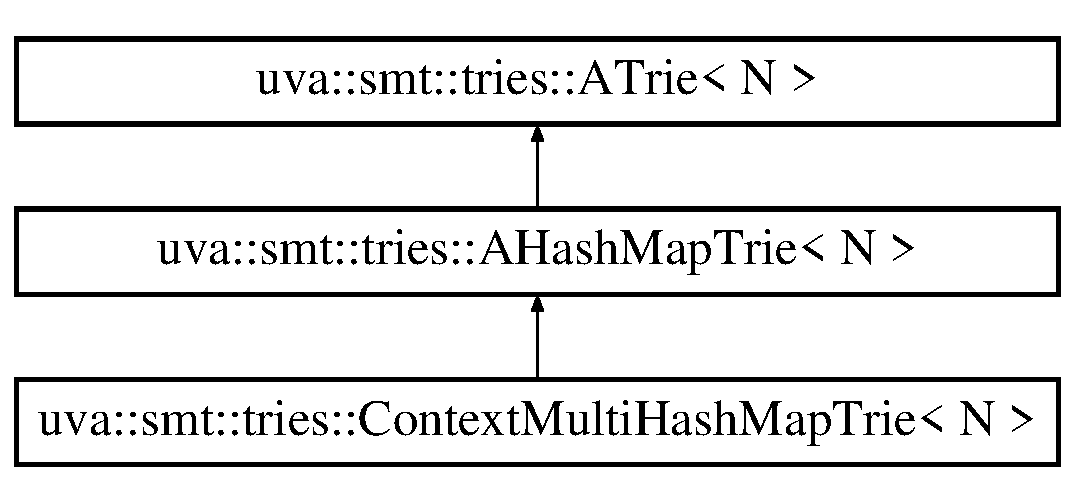
\includegraphics[height=3.000000cm]{classuva_1_1smt_1_1tries_1_1_context_multi_hash_map_trie}
\end{center}
\end{figure}
\subsection*{Public Member Functions}
\begin{DoxyCompactItemize}
\item 
\hyperlink{classuva_1_1smt_1_1tries_1_1_context_multi_hash_map_trie_a4dedd355285be9d410d0cef0faf4e493}{Context\+Multi\+Hash\+Map\+Trie} (const float \+\_\+word\+Index\+Mem\+Factor, const float \+\_\+o\+Gram\+Mem\+Factor, const float \+\_\+m\+Gram\+Mem\+Factor, const float \+\_\+n\+Gram\+Mem\+Factor)
\item 
virtual void \hyperlink{classuva_1_1smt_1_1tries_1_1_context_multi_hash_map_trie_ac744e6f6e63317d1f955ac96d504f724}{pre\+Allocate} (const size\+\_\+t counts\mbox{[}N\mbox{]})
\item 
virtual void \hyperlink{classuva_1_1smt_1_1tries_1_1_context_multi_hash_map_trie_abc5ad6e7f2a260a4cc374bbc332edc5c}{add1\+Gram} (const \hyperlink{structuva_1_1smt_1_1tries_1_1_s_back_off_n_gram}{S\+Back\+Off\+N\+Gram} \&o\+Gram)
\item 
virtual void \hyperlink{classuva_1_1smt_1_1tries_1_1_context_multi_hash_map_trie_adaf0ff4116ea8c9c0ffe7407841bf8e1}{add\+M\+Gram} (const \hyperlink{structuva_1_1smt_1_1tries_1_1_s_back_off_n_gram}{S\+Back\+Off\+N\+Gram} \&m\+Gram)
\item 
virtual void \hyperlink{classuva_1_1smt_1_1tries_1_1_context_multi_hash_map_trie_a2d8c22fa039d475b8b39f06531b58bc7}{add\+N\+Gram} (const \hyperlink{structuva_1_1smt_1_1tries_1_1_s_back_off_n_gram}{S\+Back\+Off\+N\+Gram} \&n\+Gram)
\item 
virtual void \hyperlink{classuva_1_1smt_1_1tries_1_1_context_multi_hash_map_trie_ad861e3027580ea2b78c95b22c43395ee}{query\+N\+Gram} (const vector$<$ string $>$ \&ngram, \hyperlink{structuva_1_1smt_1_1tries_1_1_s_prob_result}{S\+Prob\+Result} \&result)
\item 
virtual \hyperlink{classuva_1_1smt_1_1tries_1_1_context_multi_hash_map_trie_ad3a1ce51fea9d2c2d6aaf4f2f0dded85}{$\sim$\+Context\+Multi\+Hash\+Map\+Trie} ()
\end{DoxyCompactItemize}
\subsection*{Static Public Attributes}
\begin{DoxyCompactItemize}
\item 
static const \hyperlink{namespaceuva_1_1smt_1_1tries_a26064146e98856c7c4185efab0e61a36}{T\+Model\+Level} \hyperlink{classuva_1_1smt_1_1tries_1_1_context_multi_hash_map_trie_ab12bd7cfd0b00da7c134d8d6b1694346}{M\+G\+R\+A\+M\+\_\+\+I\+D\+X\+\_\+\+O\+F\+F\+S\+E\+T} = 2
\end{DoxyCompactItemize}
\subsection*{Additional Inherited Members}


\subsection{Detailed Description}
\subsubsection*{template$<$T\+Model\+Level N$>$class uva\+::smt\+::tries\+::\+Context\+Multi\+Hash\+Map\+Trie$<$ N $>$}

This is a Hash\+Mpa based I\+Trie interface implementation class. Note 1\+: This implementation uses the unsigned long for the hashes it is not optimal Note 2\+: the unordered\+\_\+map might be not as efficient as a hash\+\_\+map with respect to memory usage but it is supposed to be faster

This implementation is chosen because it resembles the ordered array implementation from\+: \char`\"{}\+Faster and Smaller N -\/\+Gram Language Models\char`\"{} Adam Pauls Dan Klein Computer Science Division University of California, Berkeley

and unordered\+\_\+maps showed good performance in\+: \char`\"{}\+Efficient in-\/memory data structures for n-\/grams indexing\char`\"{} Daniel Robenek, Jan Platoˇs, and V ́aclav Sn ́aˇsel Department of Computer Science, F\+E\+I, V\+S\+B – Technical University of Ostrava
\begin{DoxyEnumerate}
\item listopadu 15, 708 33, Ostrava-\/\+Poruba, Czech Republic \{daniel.\+robenek.\+st, jan.\+platos, vaclav.\+snasel\}.cz 
\end{DoxyEnumerate}

\subsection{Constructor \& Destructor Documentation}
\hypertarget{classuva_1_1smt_1_1tries_1_1_context_multi_hash_map_trie_a4dedd355285be9d410d0cef0faf4e493}{}\index{uva\+::smt\+::tries\+::\+Context\+Multi\+Hash\+Map\+Trie@{uva\+::smt\+::tries\+::\+Context\+Multi\+Hash\+Map\+Trie}!Context\+Multi\+Hash\+Map\+Trie@{Context\+Multi\+Hash\+Map\+Trie}}
\index{Context\+Multi\+Hash\+Map\+Trie@{Context\+Multi\+Hash\+Map\+Trie}!uva\+::smt\+::tries\+::\+Context\+Multi\+Hash\+Map\+Trie@{uva\+::smt\+::tries\+::\+Context\+Multi\+Hash\+Map\+Trie}}
\subsubsection[{Context\+Multi\+Hash\+Map\+Trie(const float \+\_\+word\+Index\+Mem\+Factor, const float \+\_\+o\+Gram\+Mem\+Factor, const float \+\_\+m\+Gram\+Mem\+Factor, const float \+\_\+n\+Gram\+Mem\+Factor)}]{\setlength{\rightskip}{0pt plus 5cm}template$<$T\+Model\+Level N$>$ {\bf uva\+::smt\+::tries\+::\+Context\+Multi\+Hash\+Map\+Trie}$<$ N $>$\+::{\bf Context\+Multi\+Hash\+Map\+Trie} (
\begin{DoxyParamCaption}
\item[{const float}]{\+\_\+word\+Index\+Mem\+Factor, }
\item[{const float}]{\+\_\+o\+Gram\+Mem\+Factor, }
\item[{const float}]{\+\_\+m\+Gram\+Mem\+Factor, }
\item[{const float}]{\+\_\+n\+Gram\+Mem\+Factor}
\end{DoxyParamCaption}
)\hspace{0.3cm}{\ttfamily [explicit]}}\label{classuva_1_1smt_1_1tries_1_1_context_multi_hash_map_trie_a4dedd355285be9d410d0cef0faf4e493}
The basic class constructor, accepts memory factors that are the coefficients used when pre-\/allocating memory for unordered maps.

If a factor is equal to 0.\+0 then no memory is pre-\/allocated. If the factor is equal to 1.\+0 then there is only as much preallocated as needed to store the gram entries. The latter is typically not enough as unordered\+\_\+map needs more memory for internal administration. If there is not enough memory pre-\/allocated then additional allocations will take place but it does not alway lead to more efficient memory usage. The observed behavior is that it is better to pre-\/allocate a bit more memory beforehand, than needed. This leads to less memory consumption. Depending on the type of unordered\+\_\+map key/value pair types the advised factor values are from 2.\+0 to 2.\+6. Because it can not be optimally determined beforehand, these are made constructor parameters so that they can be configured by the used. This breaks encapsulation a bit, exposing the internals, but there is no other better way, for fine tuning the memory usage.


\begin{DoxyParams}{Parameters}
{\em word\+Index\+Mem\+Factor} & the assigned memory factor for storage allocation in the unordered\+\_\+map used for the word index \\
\hline
{\em o\+Gram\+Mem\+Factor} & The One-\/\+Gram memory factor needed for the greedy allocator for the unordered\+\_\+map \\
\hline
{\em m\+Gram\+Mem\+Factor} & The M-\/\+Gram memory factor needed for the greedy allocator for the unordered\+\_\+map \\
\hline
{\em n\+Gram\+Mem\+Factor} & The N-\/\+Gram memory factor needed for the greedy allocator for the unordered\+\_\+map \\
\hline
\end{DoxyParams}
\hypertarget{classuva_1_1smt_1_1tries_1_1_context_multi_hash_map_trie_ad3a1ce51fea9d2c2d6aaf4f2f0dded85}{}\index{uva\+::smt\+::tries\+::\+Context\+Multi\+Hash\+Map\+Trie@{uva\+::smt\+::tries\+::\+Context\+Multi\+Hash\+Map\+Trie}!````~Context\+Multi\+Hash\+Map\+Trie@{$\sim$\+Context\+Multi\+Hash\+Map\+Trie}}
\index{````~Context\+Multi\+Hash\+Map\+Trie@{$\sim$\+Context\+Multi\+Hash\+Map\+Trie}!uva\+::smt\+::tries\+::\+Context\+Multi\+Hash\+Map\+Trie@{uva\+::smt\+::tries\+::\+Context\+Multi\+Hash\+Map\+Trie}}
\subsubsection[{$\sim$\+Context\+Multi\+Hash\+Map\+Trie()}]{\setlength{\rightskip}{0pt plus 5cm}template$<$T\+Model\+Level N$>$ {\bf uva\+::smt\+::tries\+::\+Context\+Multi\+Hash\+Map\+Trie}$<$ N $>$\+::$\sim${\bf Context\+Multi\+Hash\+Map\+Trie} (
\begin{DoxyParamCaption}
{}
\end{DoxyParamCaption}
)\hspace{0.3cm}{\ttfamily [virtual]}}\label{classuva_1_1smt_1_1tries_1_1_context_multi_hash_map_trie_ad3a1ce51fea9d2c2d6aaf4f2f0dded85}


\subsection{Member Function Documentation}
\hypertarget{classuva_1_1smt_1_1tries_1_1_context_multi_hash_map_trie_abc5ad6e7f2a260a4cc374bbc332edc5c}{}\index{uva\+::smt\+::tries\+::\+Context\+Multi\+Hash\+Map\+Trie@{uva\+::smt\+::tries\+::\+Context\+Multi\+Hash\+Map\+Trie}!add1\+Gram@{add1\+Gram}}
\index{add1\+Gram@{add1\+Gram}!uva\+::smt\+::tries\+::\+Context\+Multi\+Hash\+Map\+Trie@{uva\+::smt\+::tries\+::\+Context\+Multi\+Hash\+Map\+Trie}}
\subsubsection[{add1\+Gram(const S\+Back\+Off\+N\+Gram \&o\+Gram)}]{\setlength{\rightskip}{0pt plus 5cm}template$<$T\+Model\+Level N$>$ void {\bf uva\+::smt\+::tries\+::\+Context\+Multi\+Hash\+Map\+Trie}$<$ N $>$\+::add1\+Gram (
\begin{DoxyParamCaption}
\item[{const {\bf S\+Back\+Off\+N\+Gram} \&}]{o\+Gram}
\end{DoxyParamCaption}
)\hspace{0.3cm}{\ttfamily [virtual]}}\label{classuva_1_1smt_1_1tries_1_1_context_multi_hash_map_trie_abc5ad6e7f2a260a4cc374bbc332edc5c}
This method adds a 1-\/\+Gram (word) to the trie. For more details \begin{DoxySeeAlso}{See also}
I\+Trie 
\end{DoxySeeAlso}


Implements \hyperlink{classuva_1_1smt_1_1tries_1_1_a_trie_af184dbb0b095d24c76f79c7da6479eda}{uva\+::smt\+::tries\+::\+A\+Trie$<$ N $>$}.

\hypertarget{classuva_1_1smt_1_1tries_1_1_context_multi_hash_map_trie_adaf0ff4116ea8c9c0ffe7407841bf8e1}{}\index{uva\+::smt\+::tries\+::\+Context\+Multi\+Hash\+Map\+Trie@{uva\+::smt\+::tries\+::\+Context\+Multi\+Hash\+Map\+Trie}!add\+M\+Gram@{add\+M\+Gram}}
\index{add\+M\+Gram@{add\+M\+Gram}!uva\+::smt\+::tries\+::\+Context\+Multi\+Hash\+Map\+Trie@{uva\+::smt\+::tries\+::\+Context\+Multi\+Hash\+Map\+Trie}}
\subsubsection[{add\+M\+Gram(const S\+Back\+Off\+N\+Gram \&m\+Gram)}]{\setlength{\rightskip}{0pt plus 5cm}template$<$T\+Model\+Level N$>$ void {\bf uva\+::smt\+::tries\+::\+Context\+Multi\+Hash\+Map\+Trie}$<$ N $>$\+::add\+M\+Gram (
\begin{DoxyParamCaption}
\item[{const {\bf S\+Back\+Off\+N\+Gram} \&}]{m\+Gram}
\end{DoxyParamCaption}
)\hspace{0.3cm}{\ttfamily [virtual]}}\label{classuva_1_1smt_1_1tries_1_1_context_multi_hash_map_trie_adaf0ff4116ea8c9c0ffe7407841bf8e1}
This method adds a M-\/\+Gram (word) to the trie where 1 $<$ M $<$ N For more details \begin{DoxySeeAlso}{See also}
I\+Trie 
\end{DoxySeeAlso}


Implements \hyperlink{classuva_1_1smt_1_1tries_1_1_a_trie_acf62fc322ece5ec01ca00e96e17eb9ef}{uva\+::smt\+::tries\+::\+A\+Trie$<$ N $>$}.

\hypertarget{classuva_1_1smt_1_1tries_1_1_context_multi_hash_map_trie_a2d8c22fa039d475b8b39f06531b58bc7}{}\index{uva\+::smt\+::tries\+::\+Context\+Multi\+Hash\+Map\+Trie@{uva\+::smt\+::tries\+::\+Context\+Multi\+Hash\+Map\+Trie}!add\+N\+Gram@{add\+N\+Gram}}
\index{add\+N\+Gram@{add\+N\+Gram}!uva\+::smt\+::tries\+::\+Context\+Multi\+Hash\+Map\+Trie@{uva\+::smt\+::tries\+::\+Context\+Multi\+Hash\+Map\+Trie}}
\subsubsection[{add\+N\+Gram(const S\+Back\+Off\+N\+Gram \&n\+Gram)}]{\setlength{\rightskip}{0pt plus 5cm}template$<$T\+Model\+Level N$>$ void {\bf uva\+::smt\+::tries\+::\+Context\+Multi\+Hash\+Map\+Trie}$<$ N $>$\+::add\+N\+Gram (
\begin{DoxyParamCaption}
\item[{const {\bf S\+Back\+Off\+N\+Gram} \&}]{n\+Gram}
\end{DoxyParamCaption}
)\hspace{0.3cm}{\ttfamily [virtual]}}\label{classuva_1_1smt_1_1tries_1_1_context_multi_hash_map_trie_a2d8c22fa039d475b8b39f06531b58bc7}
This method adds a N-\/\+Gram (word) to the trie where For more details \begin{DoxySeeAlso}{See also}
I\+Trie 
\end{DoxySeeAlso}


Implements \hyperlink{classuva_1_1smt_1_1tries_1_1_a_trie_a240c090a5651e74304cf37b131ca9741}{uva\+::smt\+::tries\+::\+A\+Trie$<$ N $>$}.

\hypertarget{classuva_1_1smt_1_1tries_1_1_context_multi_hash_map_trie_ac744e6f6e63317d1f955ac96d504f724}{}\index{uva\+::smt\+::tries\+::\+Context\+Multi\+Hash\+Map\+Trie@{uva\+::smt\+::tries\+::\+Context\+Multi\+Hash\+Map\+Trie}!pre\+Allocate@{pre\+Allocate}}
\index{pre\+Allocate@{pre\+Allocate}!uva\+::smt\+::tries\+::\+Context\+Multi\+Hash\+Map\+Trie@{uva\+::smt\+::tries\+::\+Context\+Multi\+Hash\+Map\+Trie}}
\subsubsection[{pre\+Allocate(const size\+\_\+t counts[N])}]{\setlength{\rightskip}{0pt plus 5cm}template$<$T\+Model\+Level N$>$ void {\bf uva\+::smt\+::tries\+::\+Context\+Multi\+Hash\+Map\+Trie}$<$ N $>$\+::pre\+Allocate (
\begin{DoxyParamCaption}
\item[{const size\+\_\+t}]{counts\mbox{[}\+N\mbox{]}}
\end{DoxyParamCaption}
)\hspace{0.3cm}{\ttfamily [virtual]}}\label{classuva_1_1smt_1_1tries_1_1_context_multi_hash_map_trie_ac744e6f6e63317d1f955ac96d504f724}
This method can be used to provide the N-\/gram count information That should allow for pre-\/allocation of the memory For more details \begin{DoxySeeAlso}{See also}
I\+Trie 
\end{DoxySeeAlso}


Reimplemented from \hyperlink{classuva_1_1smt_1_1tries_1_1_a_hash_map_trie_ad867b72350326f464b563fba6727ba5f}{uva\+::smt\+::tries\+::\+A\+Hash\+Map\+Trie$<$ N $>$}.

\hypertarget{classuva_1_1smt_1_1tries_1_1_context_multi_hash_map_trie_ad861e3027580ea2b78c95b22c43395ee}{}\index{uva\+::smt\+::tries\+::\+Context\+Multi\+Hash\+Map\+Trie@{uva\+::smt\+::tries\+::\+Context\+Multi\+Hash\+Map\+Trie}!query\+N\+Gram@{query\+N\+Gram}}
\index{query\+N\+Gram@{query\+N\+Gram}!uva\+::smt\+::tries\+::\+Context\+Multi\+Hash\+Map\+Trie@{uva\+::smt\+::tries\+::\+Context\+Multi\+Hash\+Map\+Trie}}
\subsubsection[{query\+N\+Gram(const vector$<$ string $>$ \&ngram, S\+Prob\+Result \&result)}]{\setlength{\rightskip}{0pt plus 5cm}template$<$T\+Model\+Level N$>$ void {\bf uva\+::smt\+::tries\+::\+Context\+Multi\+Hash\+Map\+Trie}$<$ N $>$\+::query\+N\+Gram (
\begin{DoxyParamCaption}
\item[{const vector$<$ string $>$ \&}]{ngram, }
\item[{{\bf S\+Prob\+Result} \&}]{result}
\end{DoxyParamCaption}
)\hspace{0.3cm}{\ttfamily [virtual]}}\label{classuva_1_1smt_1_1tries_1_1_context_multi_hash_map_trie_ad861e3027580ea2b78c95b22c43395ee}
This method will get the N-\/gram in a form of a vector, e.\+g.\+: \mbox{[}word1 word2 word3 word4 word5\mbox{]} and will compute and return the Language Model Probability for it For more details \begin{DoxySeeAlso}{See also}
I\+Trie 
\end{DoxySeeAlso}


Implements \hyperlink{classuva_1_1smt_1_1tries_1_1_a_trie_a86f8301bb7a9e7a232f16bcd000062b2}{uva\+::smt\+::tries\+::\+A\+Trie$<$ N $>$}.



\subsection{Member Data Documentation}
\hypertarget{classuva_1_1smt_1_1tries_1_1_context_multi_hash_map_trie_ab12bd7cfd0b00da7c134d8d6b1694346}{}\index{uva\+::smt\+::tries\+::\+Context\+Multi\+Hash\+Map\+Trie@{uva\+::smt\+::tries\+::\+Context\+Multi\+Hash\+Map\+Trie}!M\+G\+R\+A\+M\+\_\+\+I\+D\+X\+\_\+\+O\+F\+F\+S\+E\+T@{M\+G\+R\+A\+M\+\_\+\+I\+D\+X\+\_\+\+O\+F\+F\+S\+E\+T}}
\index{M\+G\+R\+A\+M\+\_\+\+I\+D\+X\+\_\+\+O\+F\+F\+S\+E\+T@{M\+G\+R\+A\+M\+\_\+\+I\+D\+X\+\_\+\+O\+F\+F\+S\+E\+T}!uva\+::smt\+::tries\+::\+Context\+Multi\+Hash\+Map\+Trie@{uva\+::smt\+::tries\+::\+Context\+Multi\+Hash\+Map\+Trie}}
\subsubsection[{M\+G\+R\+A\+M\+\_\+\+I\+D\+X\+\_\+\+O\+F\+F\+S\+E\+T}]{\setlength{\rightskip}{0pt plus 5cm}template$<$T\+Model\+Level N$>$ const {\bf T\+Model\+Level} {\bf uva\+::smt\+::tries\+::\+Context\+Multi\+Hash\+Map\+Trie}$<$ N $>$\+::M\+G\+R\+A\+M\+\_\+\+I\+D\+X\+\_\+\+O\+F\+F\+S\+E\+T = 2\hspace{0.3cm}{\ttfamily [static]}}\label{classuva_1_1smt_1_1tries_1_1_context_multi_hash_map_trie_ab12bd7cfd0b00da7c134d8d6b1694346}


The documentation for this class was generated from the following files\+:\begin{DoxyCompactItemize}
\item 
inc/\hyperlink{_context_multi_hash_map_trie_8hpp}{Context\+Multi\+Hash\+Map\+Trie.\+hpp}\item 
src/\hyperlink{_context_multi_hash_map_trie_8cpp}{Context\+Multi\+Hash\+Map\+Trie.\+cpp}\end{DoxyCompactItemize}

\hypertarget{classuva_1_1smt_1_1exceptions_1_1_exception}{}\section{uva\+:\+:smt\+:\+:exceptions\+:\+:Exception Class Reference}
\label{classuva_1_1smt_1_1exceptions_1_1_exception}\index{uva\+::smt\+::exceptions\+::\+Exception@{uva\+::smt\+::exceptions\+::\+Exception}}


{\ttfamily \#include $<$Exceptions.\+hpp$>$}

Inheritance diagram for uva\+:\+:smt\+:\+:exceptions\+:\+:Exception\+:\begin{figure}[H]
\begin{center}
\leavevmode
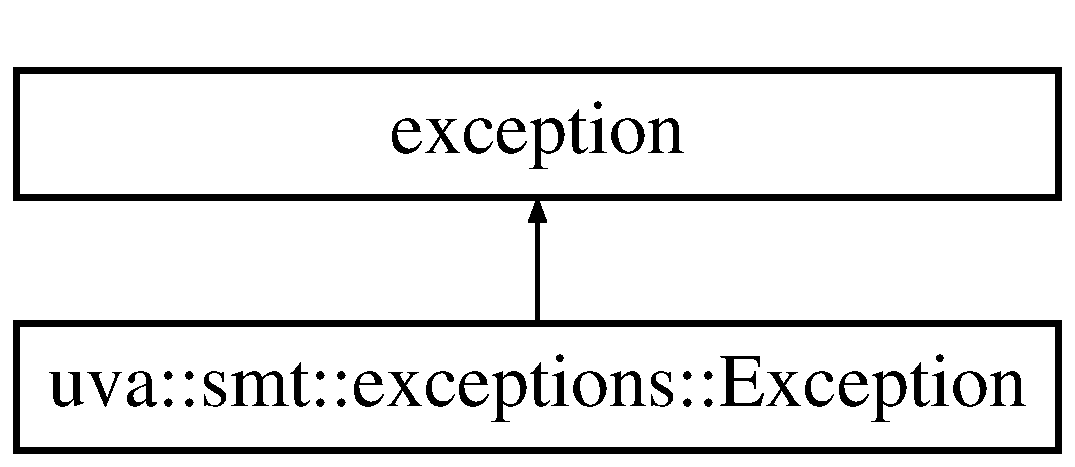
\includegraphics[height=2.000000cm]{classuva_1_1smt_1_1exceptions_1_1_exception}
\end{center}
\end{figure}
\subsection*{Public Member Functions}
\begin{DoxyCompactItemize}
\item 
\hyperlink{classuva_1_1smt_1_1exceptions_1_1_exception_a42e50b1d8a373992eb38adca8b5da8c0}{Exception} (const char $\ast$message)
\item 
\hyperlink{classuva_1_1smt_1_1exceptions_1_1_exception_a717a591b94ecbbc7f17e39b60fca3854}{Exception} (const string \&message)
\item 
\hyperlink{classuva_1_1smt_1_1exceptions_1_1_exception_a428f19e9377f8658e23f3a58251f18f4}{Exception} (\hyperlink{classuva_1_1smt_1_1exceptions_1_1_exception}{Exception} const \&other)
\item 
string const \& \hyperlink{classuva_1_1smt_1_1exceptions_1_1_exception_ad9041cffc8d5f7ca1c3f4bc9c857462c}{get\+Message} () const   throw ()
\item 
virtual \hyperlink{classuva_1_1smt_1_1exceptions_1_1_exception_a1ddbe2ffb25aca9ef031f6584af60e23}{$\sim$\+Exception} ()  throw ()
\item 
virtual const char $\ast$ \hyperlink{classuva_1_1smt_1_1exceptions_1_1_exception_a0ea6aae278f6b04d4d99a0b73befe5ee}{what} () const   throw ()
\end{DoxyCompactItemize}


\subsection{Detailed Description}
This is an application exception class that is capable of storing an error message 

\subsection{Constructor \& Destructor Documentation}
\hypertarget{classuva_1_1smt_1_1exceptions_1_1_exception_a42e50b1d8a373992eb38adca8b5da8c0}{}\index{uva\+::smt\+::exceptions\+::\+Exception@{uva\+::smt\+::exceptions\+::\+Exception}!Exception@{Exception}}
\index{Exception@{Exception}!uva\+::smt\+::exceptions\+::\+Exception@{uva\+::smt\+::exceptions\+::\+Exception}}
\subsubsection[{Exception(const char $\ast$message)}]{\setlength{\rightskip}{0pt plus 5cm}uva\+::smt\+::exceptions\+::\+Exception\+::\+Exception (
\begin{DoxyParamCaption}
\item[{const char $\ast$}]{message}
\end{DoxyParamCaption}
)\hspace{0.3cm}{\ttfamily [inline]}, {\ttfamily [explicit]}}\label{classuva_1_1smt_1_1exceptions_1_1_exception_a42e50b1d8a373992eb38adca8b5da8c0}
\hypertarget{classuva_1_1smt_1_1exceptions_1_1_exception_a717a591b94ecbbc7f17e39b60fca3854}{}\index{uva\+::smt\+::exceptions\+::\+Exception@{uva\+::smt\+::exceptions\+::\+Exception}!Exception@{Exception}}
\index{Exception@{Exception}!uva\+::smt\+::exceptions\+::\+Exception@{uva\+::smt\+::exceptions\+::\+Exception}}
\subsubsection[{Exception(const string \&message)}]{\setlength{\rightskip}{0pt plus 5cm}uva\+::smt\+::exceptions\+::\+Exception\+::\+Exception (
\begin{DoxyParamCaption}
\item[{const string \&}]{message}
\end{DoxyParamCaption}
)\hspace{0.3cm}{\ttfamily [inline]}, {\ttfamily [explicit]}}\label{classuva_1_1smt_1_1exceptions_1_1_exception_a717a591b94ecbbc7f17e39b60fca3854}
\hypertarget{classuva_1_1smt_1_1exceptions_1_1_exception_a428f19e9377f8658e23f3a58251f18f4}{}\index{uva\+::smt\+::exceptions\+::\+Exception@{uva\+::smt\+::exceptions\+::\+Exception}!Exception@{Exception}}
\index{Exception@{Exception}!uva\+::smt\+::exceptions\+::\+Exception@{uva\+::smt\+::exceptions\+::\+Exception}}
\subsubsection[{Exception(\+Exception const \&other)}]{\setlength{\rightskip}{0pt plus 5cm}uva\+::smt\+::exceptions\+::\+Exception\+::\+Exception (
\begin{DoxyParamCaption}
\item[{{\bf Exception} const \&}]{other}
\end{DoxyParamCaption}
)\hspace{0.3cm}{\ttfamily [inline]}}\label{classuva_1_1smt_1_1exceptions_1_1_exception_a428f19e9377f8658e23f3a58251f18f4}
The copy constructor 
\begin{DoxyParams}{Parameters}
{\em other} & the other exception to copy from \\
\hline
\end{DoxyParams}
\hypertarget{classuva_1_1smt_1_1exceptions_1_1_exception_a1ddbe2ffb25aca9ef031f6584af60e23}{}\index{uva\+::smt\+::exceptions\+::\+Exception@{uva\+::smt\+::exceptions\+::\+Exception}!````~Exception@{$\sim$\+Exception}}
\index{````~Exception@{$\sim$\+Exception}!uva\+::smt\+::exceptions\+::\+Exception@{uva\+::smt\+::exceptions\+::\+Exception}}
\subsubsection[{$\sim$\+Exception()}]{\setlength{\rightskip}{0pt plus 5cm}virtual uva\+::smt\+::exceptions\+::\+Exception\+::$\sim$\+Exception (
\begin{DoxyParamCaption}
{}
\end{DoxyParamCaption}
) throw  ) \hspace{0.3cm}{\ttfamily [inline]}, {\ttfamily [virtual]}}\label{classuva_1_1smt_1_1exceptions_1_1_exception_a1ddbe2ffb25aca9ef031f6584af60e23}
Destructor. Virtual to allow for subclassing. 

\subsection{Member Function Documentation}
\hypertarget{classuva_1_1smt_1_1exceptions_1_1_exception_ad9041cffc8d5f7ca1c3f4bc9c857462c}{}\index{uva\+::smt\+::exceptions\+::\+Exception@{uva\+::smt\+::exceptions\+::\+Exception}!get\+Message@{get\+Message}}
\index{get\+Message@{get\+Message}!uva\+::smt\+::exceptions\+::\+Exception@{uva\+::smt\+::exceptions\+::\+Exception}}
\subsubsection[{get\+Message() const }]{\setlength{\rightskip}{0pt plus 5cm}string const\& uva\+::smt\+::exceptions\+::\+Exception\+::get\+Message (
\begin{DoxyParamCaption}
{}
\end{DoxyParamCaption}
) const throw  ) \hspace{0.3cm}{\ttfamily [inline]}}\label{classuva_1_1smt_1_1exceptions_1_1_exception_ad9041cffc8d5f7ca1c3f4bc9c857462c}
This method returns the stored message \begin{DoxyReturn}{Returns}
the reference to a constant error message string 
\end{DoxyReturn}
\hypertarget{classuva_1_1smt_1_1exceptions_1_1_exception_a0ea6aae278f6b04d4d99a0b73befe5ee}{}\index{uva\+::smt\+::exceptions\+::\+Exception@{uva\+::smt\+::exceptions\+::\+Exception}!what@{what}}
\index{what@{what}!uva\+::smt\+::exceptions\+::\+Exception@{uva\+::smt\+::exceptions\+::\+Exception}}
\subsubsection[{what() const }]{\setlength{\rightskip}{0pt plus 5cm}virtual const char$\ast$ uva\+::smt\+::exceptions\+::\+Exception\+::what (
\begin{DoxyParamCaption}
{}
\end{DoxyParamCaption}
) const throw  ) \hspace{0.3cm}{\ttfamily [inline]}, {\ttfamily [virtual]}}\label{classuva_1_1smt_1_1exceptions_1_1_exception_a0ea6aae278f6b04d4d99a0b73befe5ee}
Returns a pointer to the (constant) error description. \begin{DoxyReturn}{Returns}
A pointer to a {\ttfamily const} {\ttfamily char$\ast$}. The underlying memory is in posession of the {\ttfamily \hyperlink{classuva_1_1smt_1_1exceptions_1_1_exception}{Exception}} object. Callers {\itshape must} not attempt to free the memory. 
\end{DoxyReturn}


The documentation for this class was generated from the following file\+:\begin{DoxyCompactItemize}
\item 
inc/\hyperlink{_exceptions_8hpp}{Exceptions.\+hpp}\end{DoxyCompactItemize}

\hypertarget{classuva_1_1smt_1_1tries_1_1alloc_1_1_greedy_memory_allocator}{}\section{uva\+:\+:smt\+:\+:tries\+:\+:alloc\+:\+:Greedy\+Memory\+Allocator$<$ T $>$ Class Template Reference}
\label{classuva_1_1smt_1_1tries_1_1alloc_1_1_greedy_memory_allocator}\index{uva\+::smt\+::tries\+::alloc\+::\+Greedy\+Memory\+Allocator$<$ T $>$@{uva\+::smt\+::tries\+::alloc\+::\+Greedy\+Memory\+Allocator$<$ T $>$}}


{\ttfamily \#include $<$Greedy\+Memory\+Allocator.\+hpp$>$}

\subsection*{Classes}
\begin{DoxyCompactItemize}
\item 
struct \hyperlink{structuva_1_1smt_1_1tries_1_1alloc_1_1_greedy_memory_allocator_1_1rebind}{rebind}
\end{DoxyCompactItemize}
\subsection*{Public Types}
\begin{DoxyCompactItemize}
\item 
typedef T \hyperlink{classuva_1_1smt_1_1tries_1_1alloc_1_1_greedy_memory_allocator_a11ff94e5a9e23e3db57976661f6d06f8}{value\+\_\+type}
\item 
typedef \hyperlink{classuva_1_1smt_1_1tries_1_1alloc_1_1_greedy_memory_storage_a15b9139bffa854a165a11131725fa903}{Greedy\+Memory\+Storage\+::size\+\_\+type} \hyperlink{classuva_1_1smt_1_1tries_1_1alloc_1_1_greedy_memory_allocator_a76d81ff5df20ef0404bb2027016b8b2d}{size\+\_\+type}
\item 
typedef std\+::ptrdiff\+\_\+t \hyperlink{classuva_1_1smt_1_1tries_1_1alloc_1_1_greedy_memory_allocator_a14467f640838b0667457750468f433cc}{difference\+\_\+type}
\item 
typedef T $\ast$ \hyperlink{classuva_1_1smt_1_1tries_1_1alloc_1_1_greedy_memory_allocator_ad82be226faea1278f210654317249483}{pointer}
\item 
typedef const T $\ast$ \hyperlink{classuva_1_1smt_1_1tries_1_1alloc_1_1_greedy_memory_allocator_aaa55b155c72c0817936b86c9c11a6ab2}{const\+\_\+pointer}
\item 
typedef T \& \hyperlink{classuva_1_1smt_1_1tries_1_1alloc_1_1_greedy_memory_allocator_a62f7001b75a49f4711f5b06900642f8b}{reference}
\item 
typedef const T \& \hyperlink{classuva_1_1smt_1_1tries_1_1alloc_1_1_greedy_memory_allocator_a1f74969c0895bf669864b2b28e675386}{const\+\_\+reference}
\end{DoxyCompactItemize}
\subsection*{Public Member Functions}
\begin{DoxyCompactItemize}
\item 
\hyperlink{classuva_1_1smt_1_1tries_1_1alloc_1_1_greedy_memory_allocator_ae87e1efb69523a746d42c2bdff324b6a}{Greedy\+Memory\+Allocator} (\hyperlink{classuva_1_1smt_1_1tries_1_1alloc_1_1_greedy_memory_allocator_a76d81ff5df20ef0404bb2027016b8b2d}{size\+\_\+type} num\+Elems)  throw ()
\item 
\hyperlink{classuva_1_1smt_1_1tries_1_1alloc_1_1_greedy_memory_allocator_a3c3e41759b86df79ce3321386b8dafcd}{Greedy\+Memory\+Allocator} (const \hyperlink{classuva_1_1smt_1_1tries_1_1alloc_1_1_greedy_memory_allocator}{Greedy\+Memory\+Allocator} \&other)  throw ()
\item 
{\footnotesize template$<$typename U $>$ }\\\hyperlink{classuva_1_1smt_1_1tries_1_1alloc_1_1_greedy_memory_allocator_afce20e748e6ecdb3890b2bb373bb755c}{Greedy\+Memory\+Allocator} (const \hyperlink{classuva_1_1smt_1_1tries_1_1alloc_1_1_greedy_memory_allocator}{Greedy\+Memory\+Allocator}$<$ U $>$ \&other)  throw ()
\item 
virtual \hyperlink{classuva_1_1smt_1_1tries_1_1alloc_1_1_greedy_memory_allocator_ad14d50375a544eb20ef5d232ab56ba85}{$\sim$\+Greedy\+Memory\+Allocator} ()  throw ()
\item 
\hyperlink{classuva_1_1smt_1_1tries_1_1alloc_1_1_greedy_memory_allocator_ad82be226faea1278f210654317249483}{pointer} \hyperlink{classuva_1_1smt_1_1tries_1_1alloc_1_1_greedy_memory_allocator_a13768ffe7599dc80f0f75bf55ddf4dbf}{address} (\hyperlink{classuva_1_1smt_1_1tries_1_1alloc_1_1_greedy_memory_allocator_a62f7001b75a49f4711f5b06900642f8b}{reference} obj) const 
\item 
\hyperlink{classuva_1_1smt_1_1tries_1_1alloc_1_1_greedy_memory_allocator_aaa55b155c72c0817936b86c9c11a6ab2}{const\+\_\+pointer} \hyperlink{classuva_1_1smt_1_1tries_1_1alloc_1_1_greedy_memory_allocator_a84868724dd7024e8a52e23bf248dfdab}{address} (\hyperlink{classuva_1_1smt_1_1tries_1_1alloc_1_1_greedy_memory_allocator_a1f74969c0895bf669864b2b28e675386}{const\+\_\+reference} obj) const 
\item 
\hyperlink{classuva_1_1smt_1_1tries_1_1alloc_1_1_greedy_memory_allocator_ad82be226faea1278f210654317249483}{pointer} \hyperlink{classuva_1_1smt_1_1tries_1_1alloc_1_1_greedy_memory_allocator_a4b1061b120ca17a9ada79050c9960134}{allocate} (\hyperlink{classuva_1_1smt_1_1tries_1_1alloc_1_1_greedy_memory_allocator_a76d81ff5df20ef0404bb2027016b8b2d}{size\+\_\+type} num, \hyperlink{classuva_1_1smt_1_1tries_1_1alloc_1_1_greedy_memory_allocator_aaa55b155c72c0817936b86c9c11a6ab2}{const\+\_\+pointer} cp=0)
\item 
void \hyperlink{classuva_1_1smt_1_1tries_1_1alloc_1_1_greedy_memory_allocator_a57550de709555d5378d86e318da7c36d}{deallocate} (\hyperlink{classuva_1_1smt_1_1tries_1_1alloc_1_1_greedy_memory_allocator_ad82be226faea1278f210654317249483}{pointer} ptr, \hyperlink{classuva_1_1smt_1_1tries_1_1alloc_1_1_greedy_memory_allocator_a76d81ff5df20ef0404bb2027016b8b2d}{size\+\_\+type} num)
\item 
\hyperlink{classuva_1_1smt_1_1tries_1_1alloc_1_1_greedy_memory_allocator_a76d81ff5df20ef0404bb2027016b8b2d}{size\+\_\+type} \hyperlink{classuva_1_1smt_1_1tries_1_1alloc_1_1_greedy_memory_allocator_a2ad3d828734f577bfbb8d85df657f15b}{available} () const   throw ()
\item 
\hyperlink{classuva_1_1smt_1_1tries_1_1alloc_1_1_greedy_memory_allocator_a76d81ff5df20ef0404bb2027016b8b2d}{size\+\_\+type} \hyperlink{classuva_1_1smt_1_1tries_1_1alloc_1_1_greedy_memory_allocator_ac749bcedee3cc0a29834feeafeca1b6a}{max\+\_\+size} () const   throw ()
\item 
void \hyperlink{classuva_1_1smt_1_1tries_1_1alloc_1_1_greedy_memory_allocator_ab734ed08724d82553b8b4a73b2d48e82}{construct} (\hyperlink{classuva_1_1smt_1_1tries_1_1alloc_1_1_greedy_memory_allocator_ad82be226faea1278f210654317249483}{pointer} ptr, const \hyperlink{classuva_1_1smt_1_1tries_1_1alloc_1_1_greedy_memory_allocator_a11ff94e5a9e23e3db57976661f6d06f8}{value\+\_\+type} \&value)
\item 
void \hyperlink{classuva_1_1smt_1_1tries_1_1alloc_1_1_greedy_memory_allocator_ac5efe3db6641f4fd16dc6d795615b86b}{destroy} (\hyperlink{classuva_1_1smt_1_1tries_1_1alloc_1_1_greedy_memory_allocator_ad82be226faea1278f210654317249483}{pointer} ptr)
\item 
\hyperlink{classuva_1_1smt_1_1tries_1_1alloc_1_1_greedy_memory_storage}{Greedy\+Memory\+Storage} \& \hyperlink{classuva_1_1smt_1_1tries_1_1alloc_1_1_greedy_memory_allocator_a84636e616956f0eec410d7f5034dbdfb}{get\+Storage\+Ref} () const 
\end{DoxyCompactItemize}
\subsection*{Protected Attributes}
\begin{DoxyCompactItemize}
\item 
\hyperlink{classuva_1_1smt_1_1tries_1_1alloc_1_1_greedy_memory_storage}{Greedy\+Memory\+Storage} \& \hyperlink{classuva_1_1smt_1_1tries_1_1alloc_1_1_greedy_memory_allocator_a43f47988468fe19dee3d5adae8574321}{\+\_\+manager}
\end{DoxyCompactItemize}


\subsection{Detailed Description}
\subsubsection*{template$<$typename T$>$class uva\+::smt\+::tries\+::alloc\+::\+Greedy\+Memory\+Allocator$<$ T $>$}

This is the fixed memory allocator class for using in the tries. Here we pre-\/allocate some fixed size memory and then just give it out when needed. Since the Trie is build once and then is not changed, we do no do any memory deallocation here! 

\subsection{Member Typedef Documentation}
\hypertarget{classuva_1_1smt_1_1tries_1_1alloc_1_1_greedy_memory_allocator_aaa55b155c72c0817936b86c9c11a6ab2}{}\index{uva\+::smt\+::tries\+::alloc\+::\+Greedy\+Memory\+Allocator@{uva\+::smt\+::tries\+::alloc\+::\+Greedy\+Memory\+Allocator}!const\+\_\+pointer@{const\+\_\+pointer}}
\index{const\+\_\+pointer@{const\+\_\+pointer}!uva\+::smt\+::tries\+::alloc\+::\+Greedy\+Memory\+Allocator@{uva\+::smt\+::tries\+::alloc\+::\+Greedy\+Memory\+Allocator}}
\subsubsection[{const\+\_\+pointer}]{\setlength{\rightskip}{0pt plus 5cm}template$<$typename T$>$ typedef const T$\ast$ {\bf uva\+::smt\+::tries\+::alloc\+::\+Greedy\+Memory\+Allocator}$<$ T $>$\+::{\bf const\+\_\+pointer}}\label{classuva_1_1smt_1_1tries_1_1alloc_1_1_greedy_memory_allocator_aaa55b155c72c0817936b86c9c11a6ab2}
\hypertarget{classuva_1_1smt_1_1tries_1_1alloc_1_1_greedy_memory_allocator_a1f74969c0895bf669864b2b28e675386}{}\index{uva\+::smt\+::tries\+::alloc\+::\+Greedy\+Memory\+Allocator@{uva\+::smt\+::tries\+::alloc\+::\+Greedy\+Memory\+Allocator}!const\+\_\+reference@{const\+\_\+reference}}
\index{const\+\_\+reference@{const\+\_\+reference}!uva\+::smt\+::tries\+::alloc\+::\+Greedy\+Memory\+Allocator@{uva\+::smt\+::tries\+::alloc\+::\+Greedy\+Memory\+Allocator}}
\subsubsection[{const\+\_\+reference}]{\setlength{\rightskip}{0pt plus 5cm}template$<$typename T$>$ typedef const T\& {\bf uva\+::smt\+::tries\+::alloc\+::\+Greedy\+Memory\+Allocator}$<$ T $>$\+::{\bf const\+\_\+reference}}\label{classuva_1_1smt_1_1tries_1_1alloc_1_1_greedy_memory_allocator_a1f74969c0895bf669864b2b28e675386}
\hypertarget{classuva_1_1smt_1_1tries_1_1alloc_1_1_greedy_memory_allocator_a14467f640838b0667457750468f433cc}{}\index{uva\+::smt\+::tries\+::alloc\+::\+Greedy\+Memory\+Allocator@{uva\+::smt\+::tries\+::alloc\+::\+Greedy\+Memory\+Allocator}!difference\+\_\+type@{difference\+\_\+type}}
\index{difference\+\_\+type@{difference\+\_\+type}!uva\+::smt\+::tries\+::alloc\+::\+Greedy\+Memory\+Allocator@{uva\+::smt\+::tries\+::alloc\+::\+Greedy\+Memory\+Allocator}}
\subsubsection[{difference\+\_\+type}]{\setlength{\rightskip}{0pt plus 5cm}template$<$typename T$>$ typedef std\+::ptrdiff\+\_\+t {\bf uva\+::smt\+::tries\+::alloc\+::\+Greedy\+Memory\+Allocator}$<$ T $>$\+::{\bf difference\+\_\+type}}\label{classuva_1_1smt_1_1tries_1_1alloc_1_1_greedy_memory_allocator_a14467f640838b0667457750468f433cc}
\hypertarget{classuva_1_1smt_1_1tries_1_1alloc_1_1_greedy_memory_allocator_ad82be226faea1278f210654317249483}{}\index{uva\+::smt\+::tries\+::alloc\+::\+Greedy\+Memory\+Allocator@{uva\+::smt\+::tries\+::alloc\+::\+Greedy\+Memory\+Allocator}!pointer@{pointer}}
\index{pointer@{pointer}!uva\+::smt\+::tries\+::alloc\+::\+Greedy\+Memory\+Allocator@{uva\+::smt\+::tries\+::alloc\+::\+Greedy\+Memory\+Allocator}}
\subsubsection[{pointer}]{\setlength{\rightskip}{0pt plus 5cm}template$<$typename T$>$ typedef T$\ast$ {\bf uva\+::smt\+::tries\+::alloc\+::\+Greedy\+Memory\+Allocator}$<$ T $>$\+::{\bf pointer}}\label{classuva_1_1smt_1_1tries_1_1alloc_1_1_greedy_memory_allocator_ad82be226faea1278f210654317249483}
\hypertarget{classuva_1_1smt_1_1tries_1_1alloc_1_1_greedy_memory_allocator_a62f7001b75a49f4711f5b06900642f8b}{}\index{uva\+::smt\+::tries\+::alloc\+::\+Greedy\+Memory\+Allocator@{uva\+::smt\+::tries\+::alloc\+::\+Greedy\+Memory\+Allocator}!reference@{reference}}
\index{reference@{reference}!uva\+::smt\+::tries\+::alloc\+::\+Greedy\+Memory\+Allocator@{uva\+::smt\+::tries\+::alloc\+::\+Greedy\+Memory\+Allocator}}
\subsubsection[{reference}]{\setlength{\rightskip}{0pt plus 5cm}template$<$typename T$>$ typedef T\& {\bf uva\+::smt\+::tries\+::alloc\+::\+Greedy\+Memory\+Allocator}$<$ T $>$\+::{\bf reference}}\label{classuva_1_1smt_1_1tries_1_1alloc_1_1_greedy_memory_allocator_a62f7001b75a49f4711f5b06900642f8b}
\hypertarget{classuva_1_1smt_1_1tries_1_1alloc_1_1_greedy_memory_allocator_a76d81ff5df20ef0404bb2027016b8b2d}{}\index{uva\+::smt\+::tries\+::alloc\+::\+Greedy\+Memory\+Allocator@{uva\+::smt\+::tries\+::alloc\+::\+Greedy\+Memory\+Allocator}!size\+\_\+type@{size\+\_\+type}}
\index{size\+\_\+type@{size\+\_\+type}!uva\+::smt\+::tries\+::alloc\+::\+Greedy\+Memory\+Allocator@{uva\+::smt\+::tries\+::alloc\+::\+Greedy\+Memory\+Allocator}}
\subsubsection[{size\+\_\+type}]{\setlength{\rightskip}{0pt plus 5cm}template$<$typename T$>$ typedef {\bf Greedy\+Memory\+Storage\+::size\+\_\+type} {\bf uva\+::smt\+::tries\+::alloc\+::\+Greedy\+Memory\+Allocator}$<$ T $>$\+::{\bf size\+\_\+type}}\label{classuva_1_1smt_1_1tries_1_1alloc_1_1_greedy_memory_allocator_a76d81ff5df20ef0404bb2027016b8b2d}
\hypertarget{classuva_1_1smt_1_1tries_1_1alloc_1_1_greedy_memory_allocator_a11ff94e5a9e23e3db57976661f6d06f8}{}\index{uva\+::smt\+::tries\+::alloc\+::\+Greedy\+Memory\+Allocator@{uva\+::smt\+::tries\+::alloc\+::\+Greedy\+Memory\+Allocator}!value\+\_\+type@{value\+\_\+type}}
\index{value\+\_\+type@{value\+\_\+type}!uva\+::smt\+::tries\+::alloc\+::\+Greedy\+Memory\+Allocator@{uva\+::smt\+::tries\+::alloc\+::\+Greedy\+Memory\+Allocator}}
\subsubsection[{value\+\_\+type}]{\setlength{\rightskip}{0pt plus 5cm}template$<$typename T$>$ typedef T {\bf uva\+::smt\+::tries\+::alloc\+::\+Greedy\+Memory\+Allocator}$<$ T $>$\+::{\bf value\+\_\+type}}\label{classuva_1_1smt_1_1tries_1_1alloc_1_1_greedy_memory_allocator_a11ff94e5a9e23e3db57976661f6d06f8}


\subsection{Constructor \& Destructor Documentation}
\hypertarget{classuva_1_1smt_1_1tries_1_1alloc_1_1_greedy_memory_allocator_ae87e1efb69523a746d42c2bdff324b6a}{}\index{uva\+::smt\+::tries\+::alloc\+::\+Greedy\+Memory\+Allocator@{uva\+::smt\+::tries\+::alloc\+::\+Greedy\+Memory\+Allocator}!Greedy\+Memory\+Allocator@{Greedy\+Memory\+Allocator}}
\index{Greedy\+Memory\+Allocator@{Greedy\+Memory\+Allocator}!uva\+::smt\+::tries\+::alloc\+::\+Greedy\+Memory\+Allocator@{uva\+::smt\+::tries\+::alloc\+::\+Greedy\+Memory\+Allocator}}
\subsubsection[{Greedy\+Memory\+Allocator(size\+\_\+type num\+Elems)}]{\setlength{\rightskip}{0pt plus 5cm}template$<$typename T$>$ {\bf uva\+::smt\+::tries\+::alloc\+::\+Greedy\+Memory\+Allocator}$<$ T $>$\+::{\bf Greedy\+Memory\+Allocator} (
\begin{DoxyParamCaption}
\item[{{\bf size\+\_\+type}}]{num\+Elems}
\end{DoxyParamCaption}
) throw  ) \hspace{0.3cm}{\ttfamily [inline]}}\label{classuva_1_1smt_1_1tries_1_1alloc_1_1_greedy_memory_allocator_ae87e1efb69523a746d42c2bdff324b6a}
The basic constructor. 
\begin{DoxyParams}{Parameters}
{\em num\+Elems} & the number of elements of template type T to pre-\/allocate memory for. \\
\hline
\end{DoxyParams}
\hypertarget{classuva_1_1smt_1_1tries_1_1alloc_1_1_greedy_memory_allocator_a3c3e41759b86df79ce3321386b8dafcd}{}\index{uva\+::smt\+::tries\+::alloc\+::\+Greedy\+Memory\+Allocator@{uva\+::smt\+::tries\+::alloc\+::\+Greedy\+Memory\+Allocator}!Greedy\+Memory\+Allocator@{Greedy\+Memory\+Allocator}}
\index{Greedy\+Memory\+Allocator@{Greedy\+Memory\+Allocator}!uva\+::smt\+::tries\+::alloc\+::\+Greedy\+Memory\+Allocator@{uva\+::smt\+::tries\+::alloc\+::\+Greedy\+Memory\+Allocator}}
\subsubsection[{Greedy\+Memory\+Allocator(const Greedy\+Memory\+Allocator \&other)}]{\setlength{\rightskip}{0pt plus 5cm}template$<$typename T$>$ {\bf uva\+::smt\+::tries\+::alloc\+::\+Greedy\+Memory\+Allocator}$<$ T $>$\+::{\bf Greedy\+Memory\+Allocator} (
\begin{DoxyParamCaption}
\item[{const {\bf Greedy\+Memory\+Allocator}$<$ T $>$ \&}]{other}
\end{DoxyParamCaption}
) throw  ) \hspace{0.3cm}{\ttfamily [inline]}}\label{classuva_1_1smt_1_1tries_1_1alloc_1_1_greedy_memory_allocator_a3c3e41759b86df79ce3321386b8dafcd}
The basic copy constructor. \hypertarget{classuva_1_1smt_1_1tries_1_1alloc_1_1_greedy_memory_allocator_afce20e748e6ecdb3890b2bb373bb755c}{}\index{uva\+::smt\+::tries\+::alloc\+::\+Greedy\+Memory\+Allocator@{uva\+::smt\+::tries\+::alloc\+::\+Greedy\+Memory\+Allocator}!Greedy\+Memory\+Allocator@{Greedy\+Memory\+Allocator}}
\index{Greedy\+Memory\+Allocator@{Greedy\+Memory\+Allocator}!uva\+::smt\+::tries\+::alloc\+::\+Greedy\+Memory\+Allocator@{uva\+::smt\+::tries\+::alloc\+::\+Greedy\+Memory\+Allocator}}
\subsubsection[{Greedy\+Memory\+Allocator(const Greedy\+Memory\+Allocator$<$ U $>$ \&other)}]{\setlength{\rightskip}{0pt plus 5cm}template$<$typename T$>$ template$<$typename U $>$ {\bf uva\+::smt\+::tries\+::alloc\+::\+Greedy\+Memory\+Allocator}$<$ T $>$\+::{\bf Greedy\+Memory\+Allocator} (
\begin{DoxyParamCaption}
\item[{const {\bf Greedy\+Memory\+Allocator}$<$ U $>$ \&}]{other}
\end{DoxyParamCaption}
) throw  ) \hspace{0.3cm}{\ttfamily [inline]}}\label{classuva_1_1smt_1_1tries_1_1alloc_1_1_greedy_memory_allocator_afce20e748e6ecdb3890b2bb373bb755c}
The basic re-\/bind constructor. It is used internally by the container in case it needs to allocate other sort data than the stored container elements. \hypertarget{classuva_1_1smt_1_1tries_1_1alloc_1_1_greedy_memory_allocator_ad14d50375a544eb20ef5d232ab56ba85}{}\index{uva\+::smt\+::tries\+::alloc\+::\+Greedy\+Memory\+Allocator@{uva\+::smt\+::tries\+::alloc\+::\+Greedy\+Memory\+Allocator}!````~Greedy\+Memory\+Allocator@{$\sim$\+Greedy\+Memory\+Allocator}}
\index{````~Greedy\+Memory\+Allocator@{$\sim$\+Greedy\+Memory\+Allocator}!uva\+::smt\+::tries\+::alloc\+::\+Greedy\+Memory\+Allocator@{uva\+::smt\+::tries\+::alloc\+::\+Greedy\+Memory\+Allocator}}
\subsubsection[{$\sim$\+Greedy\+Memory\+Allocator()}]{\setlength{\rightskip}{0pt plus 5cm}template$<$typename T$>$ virtual {\bf uva\+::smt\+::tries\+::alloc\+::\+Greedy\+Memory\+Allocator}$<$ T $>$\+::$\sim${\bf Greedy\+Memory\+Allocator} (
\begin{DoxyParamCaption}
{}
\end{DoxyParamCaption}
) throw  ) \hspace{0.3cm}{\ttfamily [inline]}, {\ttfamily [virtual]}}\label{classuva_1_1smt_1_1tries_1_1alloc_1_1_greedy_memory_allocator_ad14d50375a544eb20ef5d232ab56ba85}
The standard destructor 

\subsection{Member Function Documentation}
\hypertarget{classuva_1_1smt_1_1tries_1_1alloc_1_1_greedy_memory_allocator_a13768ffe7599dc80f0f75bf55ddf4dbf}{}\index{uva\+::smt\+::tries\+::alloc\+::\+Greedy\+Memory\+Allocator@{uva\+::smt\+::tries\+::alloc\+::\+Greedy\+Memory\+Allocator}!address@{address}}
\index{address@{address}!uva\+::smt\+::tries\+::alloc\+::\+Greedy\+Memory\+Allocator@{uva\+::smt\+::tries\+::alloc\+::\+Greedy\+Memory\+Allocator}}
\subsubsection[{address(reference obj) const }]{\setlength{\rightskip}{0pt plus 5cm}template$<$typename T$>$ {\bf pointer} {\bf uva\+::smt\+::tries\+::alloc\+::\+Greedy\+Memory\+Allocator}$<$ T $>$\+::address (
\begin{DoxyParamCaption}
\item[{{\bf reference}}]{obj}
\end{DoxyParamCaption}
) const\hspace{0.3cm}{\ttfamily [inline]}}\label{classuva_1_1smt_1_1tries_1_1alloc_1_1_greedy_memory_allocator_a13768ffe7599dc80f0f75bf55ddf4dbf}
Computes the address of the given object 
\begin{DoxyParams}{Parameters}
{\em obj} & the object to compute the pointer of \\
\hline
\end{DoxyParams}
\begin{DoxyReturn}{Returns}
the computed pointer 
\end{DoxyReturn}
\hypertarget{classuva_1_1smt_1_1tries_1_1alloc_1_1_greedy_memory_allocator_a84868724dd7024e8a52e23bf248dfdab}{}\index{uva\+::smt\+::tries\+::alloc\+::\+Greedy\+Memory\+Allocator@{uva\+::smt\+::tries\+::alloc\+::\+Greedy\+Memory\+Allocator}!address@{address}}
\index{address@{address}!uva\+::smt\+::tries\+::alloc\+::\+Greedy\+Memory\+Allocator@{uva\+::smt\+::tries\+::alloc\+::\+Greedy\+Memory\+Allocator}}
\subsubsection[{address(const\+\_\+reference obj) const }]{\setlength{\rightskip}{0pt plus 5cm}template$<$typename T$>$ {\bf const\+\_\+pointer} {\bf uva\+::smt\+::tries\+::alloc\+::\+Greedy\+Memory\+Allocator}$<$ T $>$\+::address (
\begin{DoxyParamCaption}
\item[{{\bf const\+\_\+reference}}]{obj}
\end{DoxyParamCaption}
) const\hspace{0.3cm}{\ttfamily [inline]}}\label{classuva_1_1smt_1_1tries_1_1alloc_1_1_greedy_memory_allocator_a84868724dd7024e8a52e23bf248dfdab}
Computes the address of the given object 
\begin{DoxyParams}{Parameters}
{\em obj} & the object to compute the pointer of \\
\hline
\end{DoxyParams}
\begin{DoxyReturn}{Returns}
the computed pointer 
\end{DoxyReturn}
\hypertarget{classuva_1_1smt_1_1tries_1_1alloc_1_1_greedy_memory_allocator_a4b1061b120ca17a9ada79050c9960134}{}\index{uva\+::smt\+::tries\+::alloc\+::\+Greedy\+Memory\+Allocator@{uva\+::smt\+::tries\+::alloc\+::\+Greedy\+Memory\+Allocator}!allocate@{allocate}}
\index{allocate@{allocate}!uva\+::smt\+::tries\+::alloc\+::\+Greedy\+Memory\+Allocator@{uva\+::smt\+::tries\+::alloc\+::\+Greedy\+Memory\+Allocator}}
\subsubsection[{allocate(size\+\_\+type num, const\+\_\+pointer cp=0)}]{\setlength{\rightskip}{0pt plus 5cm}template$<$typename T$>$ {\bf pointer} {\bf uva\+::smt\+::tries\+::alloc\+::\+Greedy\+Memory\+Allocator}$<$ T $>$\+::allocate (
\begin{DoxyParamCaption}
\item[{{\bf size\+\_\+type}}]{num, }
\item[{{\bf const\+\_\+pointer}}]{cp = {\ttfamily 0}}
\end{DoxyParamCaption}
)\hspace{0.3cm}{\ttfamily [inline]}}\label{classuva_1_1smt_1_1tries_1_1alloc_1_1_greedy_memory_allocator_a4b1061b120ca17a9ada79050c9960134}
Allocates memory for the given number of objects 
\begin{DoxyParams}{Parameters}
{\em num} & the number of objects to allocate \\
\hline
{\em cp} & N\+O\+T U\+S\+E\+D \\
\hline
\end{DoxyParams}
\begin{DoxyReturn}{Returns}
the pointer to the first allocated object 
\end{DoxyReturn}
\hypertarget{classuva_1_1smt_1_1tries_1_1alloc_1_1_greedy_memory_allocator_a2ad3d828734f577bfbb8d85df657f15b}{}\index{uva\+::smt\+::tries\+::alloc\+::\+Greedy\+Memory\+Allocator@{uva\+::smt\+::tries\+::alloc\+::\+Greedy\+Memory\+Allocator}!available@{available}}
\index{available@{available}!uva\+::smt\+::tries\+::alloc\+::\+Greedy\+Memory\+Allocator@{uva\+::smt\+::tries\+::alloc\+::\+Greedy\+Memory\+Allocator}}
\subsubsection[{available() const }]{\setlength{\rightskip}{0pt plus 5cm}template$<$typename T$>$ {\bf size\+\_\+type} {\bf uva\+::smt\+::tries\+::alloc\+::\+Greedy\+Memory\+Allocator}$<$ T $>$\+::available (
\begin{DoxyParamCaption}
{}
\end{DoxyParamCaption}
) const throw  ) \hspace{0.3cm}{\ttfamily [inline]}}\label{classuva_1_1smt_1_1tries_1_1alloc_1_1_greedy_memory_allocator_a2ad3d828734f577bfbb8d85df657f15b}
Returns the available number of free elements we can store \begin{DoxyReturn}{Returns}
the available number of free elements we can store 
\end{DoxyReturn}
\hypertarget{classuva_1_1smt_1_1tries_1_1alloc_1_1_greedy_memory_allocator_ab734ed08724d82553b8b4a73b2d48e82}{}\index{uva\+::smt\+::tries\+::alloc\+::\+Greedy\+Memory\+Allocator@{uva\+::smt\+::tries\+::alloc\+::\+Greedy\+Memory\+Allocator}!construct@{construct}}
\index{construct@{construct}!uva\+::smt\+::tries\+::alloc\+::\+Greedy\+Memory\+Allocator@{uva\+::smt\+::tries\+::alloc\+::\+Greedy\+Memory\+Allocator}}
\subsubsection[{construct(pointer ptr, const value\+\_\+type \&value)}]{\setlength{\rightskip}{0pt plus 5cm}template$<$typename T$>$ void {\bf uva\+::smt\+::tries\+::alloc\+::\+Greedy\+Memory\+Allocator}$<$ T $>$\+::construct (
\begin{DoxyParamCaption}
\item[{{\bf pointer}}]{ptr, }
\item[{const {\bf value\+\_\+type} \&}]{value}
\end{DoxyParamCaption}
)\hspace{0.3cm}{\ttfamily [inline]}}\label{classuva_1_1smt_1_1tries_1_1alloc_1_1_greedy_memory_allocator_ab734ed08724d82553b8b4a73b2d48e82}
Calling the constructor on the given pointer 
\begin{DoxyParams}{Parameters}
{\em ptr} & the pointer to work with \\
\hline
{\em value} & the type value to work with \\
\hline
\end{DoxyParams}
\hypertarget{classuva_1_1smt_1_1tries_1_1alloc_1_1_greedy_memory_allocator_a57550de709555d5378d86e318da7c36d}{}\index{uva\+::smt\+::tries\+::alloc\+::\+Greedy\+Memory\+Allocator@{uva\+::smt\+::tries\+::alloc\+::\+Greedy\+Memory\+Allocator}!deallocate@{deallocate}}
\index{deallocate@{deallocate}!uva\+::smt\+::tries\+::alloc\+::\+Greedy\+Memory\+Allocator@{uva\+::smt\+::tries\+::alloc\+::\+Greedy\+Memory\+Allocator}}
\subsubsection[{deallocate(pointer ptr, size\+\_\+type num)}]{\setlength{\rightskip}{0pt plus 5cm}template$<$typename T$>$ void {\bf uva\+::smt\+::tries\+::alloc\+::\+Greedy\+Memory\+Allocator}$<$ T $>$\+::deallocate (
\begin{DoxyParamCaption}
\item[{{\bf pointer}}]{ptr, }
\item[{{\bf size\+\_\+type}}]{num}
\end{DoxyParamCaption}
)\hspace{0.3cm}{\ttfamily [inline]}}\label{classuva_1_1smt_1_1tries_1_1alloc_1_1_greedy_memory_allocator_a57550de709555d5378d86e318da7c36d}
This function is supposed to deallocate the memory. We do not do that as this is fixed memory allocator 
\begin{DoxyParams}{Parameters}
{\em ptr} & the pointer to free memory from \\
\hline
{\em num} & the number of objects to deallocate \\
\hline
\end{DoxyParams}
\hypertarget{classuva_1_1smt_1_1tries_1_1alloc_1_1_greedy_memory_allocator_ac5efe3db6641f4fd16dc6d795615b86b}{}\index{uva\+::smt\+::tries\+::alloc\+::\+Greedy\+Memory\+Allocator@{uva\+::smt\+::tries\+::alloc\+::\+Greedy\+Memory\+Allocator}!destroy@{destroy}}
\index{destroy@{destroy}!uva\+::smt\+::tries\+::alloc\+::\+Greedy\+Memory\+Allocator@{uva\+::smt\+::tries\+::alloc\+::\+Greedy\+Memory\+Allocator}}
\subsubsection[{destroy(pointer ptr)}]{\setlength{\rightskip}{0pt plus 5cm}template$<$typename T$>$ void {\bf uva\+::smt\+::tries\+::alloc\+::\+Greedy\+Memory\+Allocator}$<$ T $>$\+::destroy (
\begin{DoxyParamCaption}
\item[{{\bf pointer}}]{ptr}
\end{DoxyParamCaption}
)\hspace{0.3cm}{\ttfamily [inline]}}\label{classuva_1_1smt_1_1tries_1_1alloc_1_1_greedy_memory_allocator_ac5efe3db6641f4fd16dc6d795615b86b}
Calling the destructor on the given pointer 
\begin{DoxyParams}{Parameters}
{\em ptr} & the pointer to work with \\
\hline
\end{DoxyParams}
\hypertarget{classuva_1_1smt_1_1tries_1_1alloc_1_1_greedy_memory_allocator_a84636e616956f0eec410d7f5034dbdfb}{}\index{uva\+::smt\+::tries\+::alloc\+::\+Greedy\+Memory\+Allocator@{uva\+::smt\+::tries\+::alloc\+::\+Greedy\+Memory\+Allocator}!get\+Storage\+Ref@{get\+Storage\+Ref}}
\index{get\+Storage\+Ref@{get\+Storage\+Ref}!uva\+::smt\+::tries\+::alloc\+::\+Greedy\+Memory\+Allocator@{uva\+::smt\+::tries\+::alloc\+::\+Greedy\+Memory\+Allocator}}
\subsubsection[{get\+Storage\+Ref() const }]{\setlength{\rightskip}{0pt plus 5cm}template$<$typename T$>$ {\bf Greedy\+Memory\+Storage}\& {\bf uva\+::smt\+::tries\+::alloc\+::\+Greedy\+Memory\+Allocator}$<$ T $>$\+::get\+Storage\+Ref (
\begin{DoxyParamCaption}
{}
\end{DoxyParamCaption}
) const\hspace{0.3cm}{\ttfamily [inline]}}\label{classuva_1_1smt_1_1tries_1_1alloc_1_1_greedy_memory_allocator_a84636e616956f0eec410d7f5034dbdfb}
Returns the reference to the buffer manager \begin{DoxyReturn}{Returns}
the reference to the buffer manager 
\end{DoxyReturn}
\hypertarget{classuva_1_1smt_1_1tries_1_1alloc_1_1_greedy_memory_allocator_ac749bcedee3cc0a29834feeafeca1b6a}{}\index{uva\+::smt\+::tries\+::alloc\+::\+Greedy\+Memory\+Allocator@{uva\+::smt\+::tries\+::alloc\+::\+Greedy\+Memory\+Allocator}!max\+\_\+size@{max\+\_\+size}}
\index{max\+\_\+size@{max\+\_\+size}!uva\+::smt\+::tries\+::alloc\+::\+Greedy\+Memory\+Allocator@{uva\+::smt\+::tries\+::alloc\+::\+Greedy\+Memory\+Allocator}}
\subsubsection[{max\+\_\+size() const }]{\setlength{\rightskip}{0pt plus 5cm}template$<$typename T$>$ {\bf size\+\_\+type} {\bf uva\+::smt\+::tries\+::alloc\+::\+Greedy\+Memory\+Allocator}$<$ T $>$\+::max\+\_\+size (
\begin{DoxyParamCaption}
{}
\end{DoxyParamCaption}
) const throw  ) \hspace{0.3cm}{\ttfamily [inline]}}\label{classuva_1_1smt_1_1tries_1_1alloc_1_1_greedy_memory_allocator_ac749bcedee3cc0a29834feeafeca1b6a}
Returns the maximum number of elements we can store \begin{DoxyReturn}{Returns}
the maximum number of elements we can store 
\end{DoxyReturn}


\subsection{Member Data Documentation}
\hypertarget{classuva_1_1smt_1_1tries_1_1alloc_1_1_greedy_memory_allocator_a43f47988468fe19dee3d5adae8574321}{}\index{uva\+::smt\+::tries\+::alloc\+::\+Greedy\+Memory\+Allocator@{uva\+::smt\+::tries\+::alloc\+::\+Greedy\+Memory\+Allocator}!\+\_\+manager@{\+\_\+manager}}
\index{\+\_\+manager@{\+\_\+manager}!uva\+::smt\+::tries\+::alloc\+::\+Greedy\+Memory\+Allocator@{uva\+::smt\+::tries\+::alloc\+::\+Greedy\+Memory\+Allocator}}
\subsubsection[{\+\_\+manager}]{\setlength{\rightskip}{0pt plus 5cm}template$<$typename T$>$ {\bf Greedy\+Memory\+Storage}\& {\bf uva\+::smt\+::tries\+::alloc\+::\+Greedy\+Memory\+Allocator}$<$ T $>$\+::\+\_\+manager\hspace{0.3cm}{\ttfamily [protected]}}\label{classuva_1_1smt_1_1tries_1_1alloc_1_1_greedy_memory_allocator_a43f47988468fe19dee3d5adae8574321}


The documentation for this class was generated from the following file\+:\begin{DoxyCompactItemize}
\item 
inc/\hyperlink{_greedy_memory_allocator_8hpp}{Greedy\+Memory\+Allocator.\+hpp}\end{DoxyCompactItemize}

\hypertarget{classuva_1_1smt_1_1tries_1_1alloc_1_1_greedy_memory_storage}{}\section{uva\+:\+:smt\+:\+:tries\+:\+:alloc\+:\+:Greedy\+Memory\+Storage Class Reference}
\label{classuva_1_1smt_1_1tries_1_1alloc_1_1_greedy_memory_storage}\index{uva\+::smt\+::tries\+::alloc\+::\+Greedy\+Memory\+Storage@{uva\+::smt\+::tries\+::alloc\+::\+Greedy\+Memory\+Storage}}


{\ttfamily \#include $<$Greedy\+Memory\+Storage.\+hpp$>$}

\subsection*{Public Types}
\begin{DoxyCompactItemize}
\item 
typedef uint8\+\_\+t \hyperlink{classuva_1_1smt_1_1tries_1_1alloc_1_1_greedy_memory_storage_a382ab7e2f6a10ec5da8de9d836f34f32}{T\+Storage\+Data}
\item 
typedef std\+::size\+\_\+t \hyperlink{classuva_1_1smt_1_1tries_1_1alloc_1_1_greedy_memory_storage_a15b9139bffa854a165a11131725fa903}{size\+\_\+type}
\end{DoxyCompactItemize}
\subsection*{Public Member Functions}
\begin{DoxyCompactItemize}
\item 
\hyperlink{classuva_1_1smt_1_1tries_1_1alloc_1_1_greedy_memory_storage_ad884058f655d984fd2020d2f78ebfae1}{Greedy\+Memory\+Storage} ()
\item 
\hyperlink{classuva_1_1smt_1_1tries_1_1alloc_1_1_greedy_memory_storage_adf64473bd3554e6a99ee76eaa8f5bb86}{Greedy\+Memory\+Storage} (\hyperlink{classuva_1_1smt_1_1tries_1_1alloc_1_1_greedy_memory_storage_a15b9139bffa854a165a11131725fa903}{size\+\_\+type} num\+Bytes)
\item 
\hyperlink{classuva_1_1smt_1_1tries_1_1alloc_1_1_greedy_memory_storage_a9f6bc53f9409b7e33cbd71b049e84b62}{Greedy\+Memory\+Storage} (const \hyperlink{classuva_1_1smt_1_1tries_1_1alloc_1_1_greedy_memory_storage}{Greedy\+Memory\+Storage} \&source)
\item 
\hyperlink{classuva_1_1smt_1_1tries_1_1alloc_1_1_greedy_memory_storage_a1989fe7f8ce7a1d5a6eb5099a7f758a3}{$\sim$\+Greedy\+Memory\+Storage} ()
\item 
\hyperlink{classuva_1_1smt_1_1tries_1_1alloc_1_1_greedy_memory_storage_a15b9139bffa854a165a11131725fa903}{size\+\_\+type} \hyperlink{classuva_1_1smt_1_1tries_1_1alloc_1_1_greedy_memory_storage_a15e65cfaa69595d51abf6d0218a0b61e}{get\+Buffer\+Size\+Bytes} () const 
\item 
\hyperlink{classuva_1_1smt_1_1tries_1_1alloc_1_1_greedy_memory_storage_a15b9139bffa854a165a11131725fa903}{size\+\_\+type} \hyperlink{classuva_1_1smt_1_1tries_1_1alloc_1_1_greedy_memory_storage_a4f9ace52a4b63a18d93860adf2d227bb}{get\+Available\+Bytes} () const 
\item 
void $\ast$ \hyperlink{classuva_1_1smt_1_1tries_1_1alloc_1_1_greedy_memory_storage_a796730fda3574ac4654bed1e12b1117d}{allocate} (\hyperlink{classuva_1_1smt_1_1tries_1_1alloc_1_1_greedy_memory_storage_a15b9139bffa854a165a11131725fa903}{size\+\_\+type} num)
\end{DoxyCompactItemize}
\subsection*{Protected Attributes}
\begin{DoxyCompactItemize}
\item 
void $\ast$ \hyperlink{classuva_1_1smt_1_1tries_1_1alloc_1_1_greedy_memory_storage_a1c8ad9025dcdf7c396b72cb06a67662a}{\+\_\+p\+Buffer}
\item 
vector$<$ void $\ast$ $>$ \hyperlink{classuva_1_1smt_1_1tries_1_1alloc_1_1_greedy_memory_storage_a98f1adcd062b5d194b7a4a6053abf539}{\+\_\+memory\+Buffers}
\item 
\hyperlink{classuva_1_1smt_1_1tries_1_1alloc_1_1_greedy_memory_storage_a15b9139bffa854a165a11131725fa903}{size\+\_\+type} \hyperlink{classuva_1_1smt_1_1tries_1_1alloc_1_1_greedy_memory_storage_a256828860dc5ada542a90c80c3f8753d}{\+\_\+num\+Bytes}
\item 
\hyperlink{classuva_1_1smt_1_1tries_1_1alloc_1_1_greedy_memory_storage_a15b9139bffa854a165a11131725fa903}{size\+\_\+type} \hyperlink{classuva_1_1smt_1_1tries_1_1alloc_1_1_greedy_memory_storage_a7364ad54922d2866d881cada8d29017f}{\+\_\+alloc\+Bytes}
\end{DoxyCompactItemize}


\subsection{Detailed Description}
This is the greedy memory storage class that in the first place allocates some storage and then only grows it if more space is needed! 

\subsection{Member Typedef Documentation}
\hypertarget{classuva_1_1smt_1_1tries_1_1alloc_1_1_greedy_memory_storage_a15b9139bffa854a165a11131725fa903}{}\index{uva\+::smt\+::tries\+::alloc\+::\+Greedy\+Memory\+Storage@{uva\+::smt\+::tries\+::alloc\+::\+Greedy\+Memory\+Storage}!size\+\_\+type@{size\+\_\+type}}
\index{size\+\_\+type@{size\+\_\+type}!uva\+::smt\+::tries\+::alloc\+::\+Greedy\+Memory\+Storage@{uva\+::smt\+::tries\+::alloc\+::\+Greedy\+Memory\+Storage}}
\subsubsection[{size\+\_\+type}]{\setlength{\rightskip}{0pt plus 5cm}typedef std\+::size\+\_\+t {\bf uva\+::smt\+::tries\+::alloc\+::\+Greedy\+Memory\+Storage\+::size\+\_\+type}}\label{classuva_1_1smt_1_1tries_1_1alloc_1_1_greedy_memory_storage_a15b9139bffa854a165a11131725fa903}
\hypertarget{classuva_1_1smt_1_1tries_1_1alloc_1_1_greedy_memory_storage_a382ab7e2f6a10ec5da8de9d836f34f32}{}\index{uva\+::smt\+::tries\+::alloc\+::\+Greedy\+Memory\+Storage@{uva\+::smt\+::tries\+::alloc\+::\+Greedy\+Memory\+Storage}!T\+Storage\+Data@{T\+Storage\+Data}}
\index{T\+Storage\+Data@{T\+Storage\+Data}!uva\+::smt\+::tries\+::alloc\+::\+Greedy\+Memory\+Storage@{uva\+::smt\+::tries\+::alloc\+::\+Greedy\+Memory\+Storage}}
\subsubsection[{T\+Storage\+Data}]{\setlength{\rightskip}{0pt plus 5cm}typedef uint8\+\_\+t {\bf uva\+::smt\+::tries\+::alloc\+::\+Greedy\+Memory\+Storage\+::\+T\+Storage\+Data}}\label{classuva_1_1smt_1_1tries_1_1alloc_1_1_greedy_memory_storage_a382ab7e2f6a10ec5da8de9d836f34f32}


\subsection{Constructor \& Destructor Documentation}
\hypertarget{classuva_1_1smt_1_1tries_1_1alloc_1_1_greedy_memory_storage_ad884058f655d984fd2020d2f78ebfae1}{}\index{uva\+::smt\+::tries\+::alloc\+::\+Greedy\+Memory\+Storage@{uva\+::smt\+::tries\+::alloc\+::\+Greedy\+Memory\+Storage}!Greedy\+Memory\+Storage@{Greedy\+Memory\+Storage}}
\index{Greedy\+Memory\+Storage@{Greedy\+Memory\+Storage}!uva\+::smt\+::tries\+::alloc\+::\+Greedy\+Memory\+Storage@{uva\+::smt\+::tries\+::alloc\+::\+Greedy\+Memory\+Storage}}
\subsubsection[{Greedy\+Memory\+Storage()}]{\setlength{\rightskip}{0pt plus 5cm}uva\+::smt\+::tries\+::alloc\+::\+Greedy\+Memory\+Storage\+::\+Greedy\+Memory\+Storage (
\begin{DoxyParamCaption}
{}
\end{DoxyParamCaption}
)\hspace{0.3cm}{\ttfamily [inline]}, {\ttfamily [explicit]}}\label{classuva_1_1smt_1_1tries_1_1alloc_1_1_greedy_memory_storage_ad884058f655d984fd2020d2f78ebfae1}
The basic constructor \hypertarget{classuva_1_1smt_1_1tries_1_1alloc_1_1_greedy_memory_storage_adf64473bd3554e6a99ee76eaa8f5bb86}{}\index{uva\+::smt\+::tries\+::alloc\+::\+Greedy\+Memory\+Storage@{uva\+::smt\+::tries\+::alloc\+::\+Greedy\+Memory\+Storage}!Greedy\+Memory\+Storage@{Greedy\+Memory\+Storage}}
\index{Greedy\+Memory\+Storage@{Greedy\+Memory\+Storage}!uva\+::smt\+::tries\+::alloc\+::\+Greedy\+Memory\+Storage@{uva\+::smt\+::tries\+::alloc\+::\+Greedy\+Memory\+Storage}}
\subsubsection[{Greedy\+Memory\+Storage(size\+\_\+type num\+Bytes)}]{\setlength{\rightskip}{0pt plus 5cm}uva\+::smt\+::tries\+::alloc\+::\+Greedy\+Memory\+Storage\+::\+Greedy\+Memory\+Storage (
\begin{DoxyParamCaption}
\item[{{\bf size\+\_\+type}}]{num\+Bytes}
\end{DoxyParamCaption}
)\hspace{0.3cm}{\ttfamily [inline]}, {\ttfamily [explicit]}}\label{classuva_1_1smt_1_1tries_1_1alloc_1_1_greedy_memory_storage_adf64473bd3554e6a99ee76eaa8f5bb86}
The basic constructor of the greedy storage. 
\begin{DoxyParams}{Parameters}
{\em num\+Bytes} & the number of bytes to pre-\/allocate the buffer for -\/ the initial buffer capacity \\
\hline
\end{DoxyParams}
\hypertarget{classuva_1_1smt_1_1tries_1_1alloc_1_1_greedy_memory_storage_a9f6bc53f9409b7e33cbd71b049e84b62}{}\index{uva\+::smt\+::tries\+::alloc\+::\+Greedy\+Memory\+Storage@{uva\+::smt\+::tries\+::alloc\+::\+Greedy\+Memory\+Storage}!Greedy\+Memory\+Storage@{Greedy\+Memory\+Storage}}
\index{Greedy\+Memory\+Storage@{Greedy\+Memory\+Storage}!uva\+::smt\+::tries\+::alloc\+::\+Greedy\+Memory\+Storage@{uva\+::smt\+::tries\+::alloc\+::\+Greedy\+Memory\+Storage}}
\subsubsection[{Greedy\+Memory\+Storage(const Greedy\+Memory\+Storage \&source)}]{\setlength{\rightskip}{0pt plus 5cm}uva\+::smt\+::tries\+::alloc\+::\+Greedy\+Memory\+Storage\+::\+Greedy\+Memory\+Storage (
\begin{DoxyParamCaption}
\item[{const {\bf Greedy\+Memory\+Storage} \&}]{source}
\end{DoxyParamCaption}
)\hspace{0.3cm}{\ttfamily [inline]}}\label{classuva_1_1smt_1_1tries_1_1alloc_1_1_greedy_memory_storage_a9f6bc53f9409b7e33cbd71b049e84b62}
The copy constructor \hypertarget{classuva_1_1smt_1_1tries_1_1alloc_1_1_greedy_memory_storage_a1989fe7f8ce7a1d5a6eb5099a7f758a3}{}\index{uva\+::smt\+::tries\+::alloc\+::\+Greedy\+Memory\+Storage@{uva\+::smt\+::tries\+::alloc\+::\+Greedy\+Memory\+Storage}!````~Greedy\+Memory\+Storage@{$\sim$\+Greedy\+Memory\+Storage}}
\index{````~Greedy\+Memory\+Storage@{$\sim$\+Greedy\+Memory\+Storage}!uva\+::smt\+::tries\+::alloc\+::\+Greedy\+Memory\+Storage@{uva\+::smt\+::tries\+::alloc\+::\+Greedy\+Memory\+Storage}}
\subsubsection[{$\sim$\+Greedy\+Memory\+Storage()}]{\setlength{\rightskip}{0pt plus 5cm}uva\+::smt\+::tries\+::alloc\+::\+Greedy\+Memory\+Storage\+::$\sim$\+Greedy\+Memory\+Storage (
\begin{DoxyParamCaption}
{}
\end{DoxyParamCaption}
)\hspace{0.3cm}{\ttfamily [inline]}}\label{classuva_1_1smt_1_1tries_1_1alloc_1_1_greedy_memory_storage_a1989fe7f8ce7a1d5a6eb5099a7f758a3}
The basic destructor. 

\subsection{Member Function Documentation}
\hypertarget{classuva_1_1smt_1_1tries_1_1alloc_1_1_greedy_memory_storage_a796730fda3574ac4654bed1e12b1117d}{}\index{uva\+::smt\+::tries\+::alloc\+::\+Greedy\+Memory\+Storage@{uva\+::smt\+::tries\+::alloc\+::\+Greedy\+Memory\+Storage}!allocate@{allocate}}
\index{allocate@{allocate}!uva\+::smt\+::tries\+::alloc\+::\+Greedy\+Memory\+Storage@{uva\+::smt\+::tries\+::alloc\+::\+Greedy\+Memory\+Storage}}
\subsubsection[{allocate(size\+\_\+type num)}]{\setlength{\rightskip}{0pt plus 5cm}void$\ast$ uva\+::smt\+::tries\+::alloc\+::\+Greedy\+Memory\+Storage\+::allocate (
\begin{DoxyParamCaption}
\item[{{\bf size\+\_\+type}}]{num}
\end{DoxyParamCaption}
)\hspace{0.3cm}{\ttfamily [inline]}}\label{classuva_1_1smt_1_1tries_1_1alloc_1_1_greedy_memory_storage_a796730fda3574ac4654bed1e12b1117d}
Allocates the memory of required size,if there is no enough space in the buffer, then reallocates! 
\begin{DoxyParams}{Parameters}
{\em num} & the number of bytes to allocate in the buffer \\
\hline
\end{DoxyParams}
\begin{DoxyReturn}{Returns}
the pointer to the beginning of the allocated memory block 
\end{DoxyReturn}
\hypertarget{classuva_1_1smt_1_1tries_1_1alloc_1_1_greedy_memory_storage_a4f9ace52a4b63a18d93860adf2d227bb}{}\index{uva\+::smt\+::tries\+::alloc\+::\+Greedy\+Memory\+Storage@{uva\+::smt\+::tries\+::alloc\+::\+Greedy\+Memory\+Storage}!get\+Available\+Bytes@{get\+Available\+Bytes}}
\index{get\+Available\+Bytes@{get\+Available\+Bytes}!uva\+::smt\+::tries\+::alloc\+::\+Greedy\+Memory\+Storage@{uva\+::smt\+::tries\+::alloc\+::\+Greedy\+Memory\+Storage}}
\subsubsection[{get\+Available\+Bytes() const }]{\setlength{\rightskip}{0pt plus 5cm}{\bf size\+\_\+type} uva\+::smt\+::tries\+::alloc\+::\+Greedy\+Memory\+Storage\+::get\+Available\+Bytes (
\begin{DoxyParamCaption}
{}
\end{DoxyParamCaption}
) const\hspace{0.3cm}{\ttfamily [inline]}}\label{classuva_1_1smt_1_1tries_1_1alloc_1_1_greedy_memory_storage_a4f9ace52a4b63a18d93860adf2d227bb}
Returns the number of free bytes remaining \begin{DoxyReturn}{Returns}
the number of free bytes remaining 
\end{DoxyReturn}
\hypertarget{classuva_1_1smt_1_1tries_1_1alloc_1_1_greedy_memory_storage_a15e65cfaa69595d51abf6d0218a0b61e}{}\index{uva\+::smt\+::tries\+::alloc\+::\+Greedy\+Memory\+Storage@{uva\+::smt\+::tries\+::alloc\+::\+Greedy\+Memory\+Storage}!get\+Buffer\+Size\+Bytes@{get\+Buffer\+Size\+Bytes}}
\index{get\+Buffer\+Size\+Bytes@{get\+Buffer\+Size\+Bytes}!uva\+::smt\+::tries\+::alloc\+::\+Greedy\+Memory\+Storage@{uva\+::smt\+::tries\+::alloc\+::\+Greedy\+Memory\+Storage}}
\subsubsection[{get\+Buffer\+Size\+Bytes() const }]{\setlength{\rightskip}{0pt plus 5cm}{\bf size\+\_\+type} uva\+::smt\+::tries\+::alloc\+::\+Greedy\+Memory\+Storage\+::get\+Buffer\+Size\+Bytes (
\begin{DoxyParamCaption}
{}
\end{DoxyParamCaption}
) const\hspace{0.3cm}{\ttfamily [inline]}}\label{classuva_1_1smt_1_1tries_1_1alloc_1_1_greedy_memory_storage_a15e65cfaa69595d51abf6d0218a0b61e}
Returns the current buffer size \begin{DoxyReturn}{Returns}
the current buffer size 
\end{DoxyReturn}


\subsection{Member Data Documentation}
\hypertarget{classuva_1_1smt_1_1tries_1_1alloc_1_1_greedy_memory_storage_a7364ad54922d2866d881cada8d29017f}{}\index{uva\+::smt\+::tries\+::alloc\+::\+Greedy\+Memory\+Storage@{uva\+::smt\+::tries\+::alloc\+::\+Greedy\+Memory\+Storage}!\+\_\+alloc\+Bytes@{\+\_\+alloc\+Bytes}}
\index{\+\_\+alloc\+Bytes@{\+\_\+alloc\+Bytes}!uva\+::smt\+::tries\+::alloc\+::\+Greedy\+Memory\+Storage@{uva\+::smt\+::tries\+::alloc\+::\+Greedy\+Memory\+Storage}}
\subsubsection[{\+\_\+alloc\+Bytes}]{\setlength{\rightskip}{0pt plus 5cm}{\bf size\+\_\+type} uva\+::smt\+::tries\+::alloc\+::\+Greedy\+Memory\+Storage\+::\+\_\+alloc\+Bytes\hspace{0.3cm}{\ttfamily [protected]}}\label{classuva_1_1smt_1_1tries_1_1alloc_1_1_greedy_memory_storage_a7364ad54922d2866d881cada8d29017f}
\hypertarget{classuva_1_1smt_1_1tries_1_1alloc_1_1_greedy_memory_storage_a98f1adcd062b5d194b7a4a6053abf539}{}\index{uva\+::smt\+::tries\+::alloc\+::\+Greedy\+Memory\+Storage@{uva\+::smt\+::tries\+::alloc\+::\+Greedy\+Memory\+Storage}!\+\_\+memory\+Buffers@{\+\_\+memory\+Buffers}}
\index{\+\_\+memory\+Buffers@{\+\_\+memory\+Buffers}!uva\+::smt\+::tries\+::alloc\+::\+Greedy\+Memory\+Storage@{uva\+::smt\+::tries\+::alloc\+::\+Greedy\+Memory\+Storage}}
\subsubsection[{\+\_\+memory\+Buffers}]{\setlength{\rightskip}{0pt plus 5cm}vector$<$void$\ast$$>$ uva\+::smt\+::tries\+::alloc\+::\+Greedy\+Memory\+Storage\+::\+\_\+memory\+Buffers\hspace{0.3cm}{\ttfamily [protected]}}\label{classuva_1_1smt_1_1tries_1_1alloc_1_1_greedy_memory_storage_a98f1adcd062b5d194b7a4a6053abf539}
\hypertarget{classuva_1_1smt_1_1tries_1_1alloc_1_1_greedy_memory_storage_a256828860dc5ada542a90c80c3f8753d}{}\index{uva\+::smt\+::tries\+::alloc\+::\+Greedy\+Memory\+Storage@{uva\+::smt\+::tries\+::alloc\+::\+Greedy\+Memory\+Storage}!\+\_\+num\+Bytes@{\+\_\+num\+Bytes}}
\index{\+\_\+num\+Bytes@{\+\_\+num\+Bytes}!uva\+::smt\+::tries\+::alloc\+::\+Greedy\+Memory\+Storage@{uva\+::smt\+::tries\+::alloc\+::\+Greedy\+Memory\+Storage}}
\subsubsection[{\+\_\+num\+Bytes}]{\setlength{\rightskip}{0pt plus 5cm}{\bf size\+\_\+type} uva\+::smt\+::tries\+::alloc\+::\+Greedy\+Memory\+Storage\+::\+\_\+num\+Bytes\hspace{0.3cm}{\ttfamily [protected]}}\label{classuva_1_1smt_1_1tries_1_1alloc_1_1_greedy_memory_storage_a256828860dc5ada542a90c80c3f8753d}
\hypertarget{classuva_1_1smt_1_1tries_1_1alloc_1_1_greedy_memory_storage_a1c8ad9025dcdf7c396b72cb06a67662a}{}\index{uva\+::smt\+::tries\+::alloc\+::\+Greedy\+Memory\+Storage@{uva\+::smt\+::tries\+::alloc\+::\+Greedy\+Memory\+Storage}!\+\_\+p\+Buffer@{\+\_\+p\+Buffer}}
\index{\+\_\+p\+Buffer@{\+\_\+p\+Buffer}!uva\+::smt\+::tries\+::alloc\+::\+Greedy\+Memory\+Storage@{uva\+::smt\+::tries\+::alloc\+::\+Greedy\+Memory\+Storage}}
\subsubsection[{\+\_\+p\+Buffer}]{\setlength{\rightskip}{0pt plus 5cm}void$\ast$ uva\+::smt\+::tries\+::alloc\+::\+Greedy\+Memory\+Storage\+::\+\_\+p\+Buffer\hspace{0.3cm}{\ttfamily [protected]}}\label{classuva_1_1smt_1_1tries_1_1alloc_1_1_greedy_memory_storage_a1c8ad9025dcdf7c396b72cb06a67662a}


The documentation for this class was generated from the following file\+:\begin{DoxyCompactItemize}
\item 
inc/\hyperlink{_greedy_memory_storage_8hpp}{Greedy\+Memory\+Storage.\+hpp}\end{DoxyCompactItemize}

\hypertarget{classuva_1_1smt_1_1logging_1_1_logger}{}\section{uva\+:\+:smt\+:\+:logging\+:\+:Logger Class Reference}
\label{classuva_1_1smt_1_1logging_1_1_logger}\index{uva\+::smt\+::logging\+::\+Logger@{uva\+::smt\+::logging\+::\+Logger}}


{\ttfamily \#include $<$Logger.\+hpp$>$}

\subsection*{Public Types}
\begin{DoxyCompactItemize}
\item 
enum \hyperlink{classuva_1_1smt_1_1logging_1_1_logger_ad8a08f17c873112b1717d5fadbfe32d1}{Debug\+Level} \{ \\*
\hyperlink{classuva_1_1smt_1_1logging_1_1_logger_ad8a08f17c873112b1717d5fadbfe32d1ada6ecc276d8dd53e59ea137c7e4e5a8a}{U\+S\+A\+G\+E} = 0, 
\hyperlink{classuva_1_1smt_1_1logging_1_1_logger_ad8a08f17c873112b1717d5fadbfe32d1a55397e9f36c9c1d49a2b5c5f06a68205}{E\+R\+R\+O\+R} = U\+S\+A\+G\+E + 1, 
\hyperlink{classuva_1_1smt_1_1logging_1_1_logger_ad8a08f17c873112b1717d5fadbfe32d1a6ce36924e65e9fc2ead56b4aa0de74fb}{W\+A\+R\+N\+I\+N\+G} = E\+R\+R\+O\+R + 1, 
\hyperlink{classuva_1_1smt_1_1logging_1_1_logger_ad8a08f17c873112b1717d5fadbfe32d1aa7e4b44ca4abe5094a06c407d702c77e}{R\+E\+S\+U\+L\+T} = W\+A\+R\+N\+I\+N\+G + 1, 
\\*
\hyperlink{classuva_1_1smt_1_1logging_1_1_logger_ad8a08f17c873112b1717d5fadbfe32d1aa341c04184abe60847b19087e94a8cc1}{I\+N\+F\+O} = R\+E\+S\+U\+L\+T + 1, 
\hyperlink{classuva_1_1smt_1_1logging_1_1_logger_ad8a08f17c873112b1717d5fadbfe32d1a80c1a0a7d13c7c241805fe8a73720f70}{D\+E\+B\+U\+G} = I\+N\+F\+O + 1, 
\hyperlink{classuva_1_1smt_1_1logging_1_1_logger_ad8a08f17c873112b1717d5fadbfe32d1adb3f4a3acd55b0e10b40ce56054a15a8}{D\+E\+B\+U\+G1} = D\+E\+B\+U\+G + 1, 
\hyperlink{classuva_1_1smt_1_1logging_1_1_logger_ad8a08f17c873112b1717d5fadbfe32d1abd1059e3622450c09fa8c5e7187ea265}{D\+E\+B\+U\+G2} = D\+E\+B\+U\+G1 + 1, 
\\*
\hyperlink{classuva_1_1smt_1_1logging_1_1_logger_ad8a08f17c873112b1717d5fadbfe32d1a747d7f9e8625007771fde07c68088efa}{D\+E\+B\+U\+G3} = D\+E\+B\+U\+G2 + 1
 \}
\end{DoxyCompactItemize}
\subsection*{Public Member Functions}
\begin{DoxyCompactItemize}
\item 
virtual \hyperlink{classuva_1_1smt_1_1logging_1_1_logger_a3513d7db6ba5a43f59b56e3396712dbb}{$\sim$\+Logger} ()
\end{DoxyCompactItemize}
\subsection*{Static Public Member Functions}
\begin{DoxyCompactItemize}
\item 
static string \hyperlink{classuva_1_1smt_1_1logging_1_1_logger_a21c762988e07657298e025a4df2813e3}{get\+Reporting\+Levels} ()
\item 
static void \hyperlink{classuva_1_1smt_1_1logging_1_1_logger_af07617f0088beaf25775c94202144548}{set\+Reporting\+Level} (const string level)
\item 
static std\+::ostream \& \hyperlink{classuva_1_1smt_1_1logging_1_1_logger_a645d1622809b356ec5863d31666fd6fd}{Get} (\hyperlink{classuva_1_1smt_1_1logging_1_1_logger_ad8a08f17c873112b1717d5fadbfe32d1}{Debug\+Level} level)
\item 
static std\+::ostream \& \hyperlink{classuva_1_1smt_1_1logging_1_1_logger_a9e52f2be59d5ba40107135b313ea1acb}{Get} (\hyperlink{classuva_1_1smt_1_1logging_1_1_logger_ad8a08f17c873112b1717d5fadbfe32d1}{Debug\+Level} level, const char $\ast$file, const char $\ast$func, const char $\ast$line)
\item 
static \hyperlink{classuva_1_1smt_1_1logging_1_1_logger_ad8a08f17c873112b1717d5fadbfe32d1}{Debug\+Level} \& \hyperlink{classuva_1_1smt_1_1logging_1_1_logger_a48dbb0863fed63eab9ca2fc50d86bb2a}{Reporting\+Level} ()
\item 
static void \hyperlink{classuva_1_1smt_1_1logging_1_1_logger_a93e0d1e9874895360ba8a5019819a253}{start\+Progress\+Bar} ()
\item 
static void \hyperlink{classuva_1_1smt_1_1logging_1_1_logger_ac99950b42d9cbe17becae3a68f4b0015}{update\+Progress\+Bar} ()
\item 
static void \hyperlink{classuva_1_1smt_1_1logging_1_1_logger_ae71f997a95aed7402dbad289f7a0ec9f}{stop\+Progress\+Bar} ()
\item 
static bool \hyperlink{classuva_1_1smt_1_1logging_1_1_logger_adc05eba04bec4f3c46414aa6e0dd8610}{is\+Progress\+Bar\+On} ()
\end{DoxyCompactItemize}


\subsection{Detailed Description}
This is a trivial logging facility that exchibits a singleton behavior and does output to stderr and stdout. 

\subsection{Member Enumeration Documentation}
\hypertarget{classuva_1_1smt_1_1logging_1_1_logger_ad8a08f17c873112b1717d5fadbfe32d1}{}\index{uva\+::smt\+::logging\+::\+Logger@{uva\+::smt\+::logging\+::\+Logger}!Debug\+Level@{Debug\+Level}}
\index{Debug\+Level@{Debug\+Level}!uva\+::smt\+::logging\+::\+Logger@{uva\+::smt\+::logging\+::\+Logger}}
\subsubsection[{Debug\+Level}]{\setlength{\rightskip}{0pt plus 5cm}enum {\bf uva\+::smt\+::logging\+::\+Logger\+::\+Debug\+Level}}\label{classuva_1_1smt_1_1logging_1_1_logger_ad8a08f17c873112b1717d5fadbfe32d1}
\begin{Desc}
\item[Enumerator]\par
\begin{description}
\index{U\+S\+A\+G\+E@{U\+S\+A\+G\+E}!uva\+::smt\+::logging\+::\+Logger@{uva\+::smt\+::logging\+::\+Logger}}\index{uva\+::smt\+::logging\+::\+Logger@{uva\+::smt\+::logging\+::\+Logger}!U\+S\+A\+G\+E@{U\+S\+A\+G\+E}}\item[{\em 
\hypertarget{classuva_1_1smt_1_1logging_1_1_logger_ad8a08f17c873112b1717d5fadbfe32d1ada6ecc276d8dd53e59ea137c7e4e5a8a}{}U\+S\+A\+G\+E\label{classuva_1_1smt_1_1logging_1_1_logger_ad8a08f17c873112b1717d5fadbfe32d1ada6ecc276d8dd53e59ea137c7e4e5a8a}
}]\index{E\+R\+R\+O\+R@{E\+R\+R\+O\+R}!uva\+::smt\+::logging\+::\+Logger@{uva\+::smt\+::logging\+::\+Logger}}\index{uva\+::smt\+::logging\+::\+Logger@{uva\+::smt\+::logging\+::\+Logger}!E\+R\+R\+O\+R@{E\+R\+R\+O\+R}}\item[{\em 
\hypertarget{classuva_1_1smt_1_1logging_1_1_logger_ad8a08f17c873112b1717d5fadbfe32d1a55397e9f36c9c1d49a2b5c5f06a68205}{}E\+R\+R\+O\+R\label{classuva_1_1smt_1_1logging_1_1_logger_ad8a08f17c873112b1717d5fadbfe32d1a55397e9f36c9c1d49a2b5c5f06a68205}
}]\index{W\+A\+R\+N\+I\+N\+G@{W\+A\+R\+N\+I\+N\+G}!uva\+::smt\+::logging\+::\+Logger@{uva\+::smt\+::logging\+::\+Logger}}\index{uva\+::smt\+::logging\+::\+Logger@{uva\+::smt\+::logging\+::\+Logger}!W\+A\+R\+N\+I\+N\+G@{W\+A\+R\+N\+I\+N\+G}}\item[{\em 
\hypertarget{classuva_1_1smt_1_1logging_1_1_logger_ad8a08f17c873112b1717d5fadbfe32d1a6ce36924e65e9fc2ead56b4aa0de74fb}{}W\+A\+R\+N\+I\+N\+G\label{classuva_1_1smt_1_1logging_1_1_logger_ad8a08f17c873112b1717d5fadbfe32d1a6ce36924e65e9fc2ead56b4aa0de74fb}
}]\index{R\+E\+S\+U\+L\+T@{R\+E\+S\+U\+L\+T}!uva\+::smt\+::logging\+::\+Logger@{uva\+::smt\+::logging\+::\+Logger}}\index{uva\+::smt\+::logging\+::\+Logger@{uva\+::smt\+::logging\+::\+Logger}!R\+E\+S\+U\+L\+T@{R\+E\+S\+U\+L\+T}}\item[{\em 
\hypertarget{classuva_1_1smt_1_1logging_1_1_logger_ad8a08f17c873112b1717d5fadbfe32d1aa7e4b44ca4abe5094a06c407d702c77e}{}R\+E\+S\+U\+L\+T\label{classuva_1_1smt_1_1logging_1_1_logger_ad8a08f17c873112b1717d5fadbfe32d1aa7e4b44ca4abe5094a06c407d702c77e}
}]\index{I\+N\+F\+O@{I\+N\+F\+O}!uva\+::smt\+::logging\+::\+Logger@{uva\+::smt\+::logging\+::\+Logger}}\index{uva\+::smt\+::logging\+::\+Logger@{uva\+::smt\+::logging\+::\+Logger}!I\+N\+F\+O@{I\+N\+F\+O}}\item[{\em 
\hypertarget{classuva_1_1smt_1_1logging_1_1_logger_ad8a08f17c873112b1717d5fadbfe32d1aa341c04184abe60847b19087e94a8cc1}{}I\+N\+F\+O\label{classuva_1_1smt_1_1logging_1_1_logger_ad8a08f17c873112b1717d5fadbfe32d1aa341c04184abe60847b19087e94a8cc1}
}]\index{D\+E\+B\+U\+G@{D\+E\+B\+U\+G}!uva\+::smt\+::logging\+::\+Logger@{uva\+::smt\+::logging\+::\+Logger}}\index{uva\+::smt\+::logging\+::\+Logger@{uva\+::smt\+::logging\+::\+Logger}!D\+E\+B\+U\+G@{D\+E\+B\+U\+G}}\item[{\em 
\hypertarget{classuva_1_1smt_1_1logging_1_1_logger_ad8a08f17c873112b1717d5fadbfe32d1a80c1a0a7d13c7c241805fe8a73720f70}{}D\+E\+B\+U\+G\label{classuva_1_1smt_1_1logging_1_1_logger_ad8a08f17c873112b1717d5fadbfe32d1a80c1a0a7d13c7c241805fe8a73720f70}
}]\index{D\+E\+B\+U\+G1@{D\+E\+B\+U\+G1}!uva\+::smt\+::logging\+::\+Logger@{uva\+::smt\+::logging\+::\+Logger}}\index{uva\+::smt\+::logging\+::\+Logger@{uva\+::smt\+::logging\+::\+Logger}!D\+E\+B\+U\+G1@{D\+E\+B\+U\+G1}}\item[{\em 
\hypertarget{classuva_1_1smt_1_1logging_1_1_logger_ad8a08f17c873112b1717d5fadbfe32d1adb3f4a3acd55b0e10b40ce56054a15a8}{}D\+E\+B\+U\+G1\label{classuva_1_1smt_1_1logging_1_1_logger_ad8a08f17c873112b1717d5fadbfe32d1adb3f4a3acd55b0e10b40ce56054a15a8}
}]\index{D\+E\+B\+U\+G2@{D\+E\+B\+U\+G2}!uva\+::smt\+::logging\+::\+Logger@{uva\+::smt\+::logging\+::\+Logger}}\index{uva\+::smt\+::logging\+::\+Logger@{uva\+::smt\+::logging\+::\+Logger}!D\+E\+B\+U\+G2@{D\+E\+B\+U\+G2}}\item[{\em 
\hypertarget{classuva_1_1smt_1_1logging_1_1_logger_ad8a08f17c873112b1717d5fadbfe32d1abd1059e3622450c09fa8c5e7187ea265}{}D\+E\+B\+U\+G2\label{classuva_1_1smt_1_1logging_1_1_logger_ad8a08f17c873112b1717d5fadbfe32d1abd1059e3622450c09fa8c5e7187ea265}
}]\index{D\+E\+B\+U\+G3@{D\+E\+B\+U\+G3}!uva\+::smt\+::logging\+::\+Logger@{uva\+::smt\+::logging\+::\+Logger}}\index{uva\+::smt\+::logging\+::\+Logger@{uva\+::smt\+::logging\+::\+Logger}!D\+E\+B\+U\+G3@{D\+E\+B\+U\+G3}}\item[{\em 
\hypertarget{classuva_1_1smt_1_1logging_1_1_logger_ad8a08f17c873112b1717d5fadbfe32d1a747d7f9e8625007771fde07c68088efa}{}D\+E\+B\+U\+G3\label{classuva_1_1smt_1_1logging_1_1_logger_ad8a08f17c873112b1717d5fadbfe32d1a747d7f9e8625007771fde07c68088efa}
}]\end{description}
\end{Desc}


\subsection{Constructor \& Destructor Documentation}
\hypertarget{classuva_1_1smt_1_1logging_1_1_logger_a3513d7db6ba5a43f59b56e3396712dbb}{}\index{uva\+::smt\+::logging\+::\+Logger@{uva\+::smt\+::logging\+::\+Logger}!````~Logger@{$\sim$\+Logger}}
\index{````~Logger@{$\sim$\+Logger}!uva\+::smt\+::logging\+::\+Logger@{uva\+::smt\+::logging\+::\+Logger}}
\subsubsection[{$\sim$\+Logger()}]{\setlength{\rightskip}{0pt plus 5cm}virtual uva\+::smt\+::logging\+::\+Logger\+::$\sim$\+Logger (
\begin{DoxyParamCaption}
{}
\end{DoxyParamCaption}
)\hspace{0.3cm}{\ttfamily [inline]}, {\ttfamily [virtual]}}\label{classuva_1_1smt_1_1logging_1_1_logger_a3513d7db6ba5a43f59b56e3396712dbb}


\subsection{Member Function Documentation}
\hypertarget{classuva_1_1smt_1_1logging_1_1_logger_a645d1622809b356ec5863d31666fd6fd}{}\index{uva\+::smt\+::logging\+::\+Logger@{uva\+::smt\+::logging\+::\+Logger}!Get@{Get}}
\index{Get@{Get}!uva\+::smt\+::logging\+::\+Logger@{uva\+::smt\+::logging\+::\+Logger}}
\subsubsection[{Get(\+Debug\+Level level)}]{\setlength{\rightskip}{0pt plus 5cm}static std\+::ostream\& uva\+::smt\+::logging\+::\+Logger\+::\+Get (
\begin{DoxyParamCaption}
\item[{{\bf Debug\+Level}}]{level}
\end{DoxyParamCaption}
)\hspace{0.3cm}{\ttfamily [inline]}, {\ttfamily [static]}}\label{classuva_1_1smt_1_1logging_1_1_logger_a645d1622809b356ec5863d31666fd6fd}
This methods allows to get the output stream for the given log-\/level 
\begin{DoxyParams}{Parameters}
{\em level} & the log level for the messages to print \\
\hline
\end{DoxyParams}
\begin{DoxyReturn}{Returns}
the output stream object 
\end{DoxyReturn}
\hypertarget{classuva_1_1smt_1_1logging_1_1_logger_a9e52f2be59d5ba40107135b313ea1acb}{}\index{uva\+::smt\+::logging\+::\+Logger@{uva\+::smt\+::logging\+::\+Logger}!Get@{Get}}
\index{Get@{Get}!uva\+::smt\+::logging\+::\+Logger@{uva\+::smt\+::logging\+::\+Logger}}
\subsubsection[{Get(\+Debug\+Level level, const char $\ast$file, const char $\ast$func, const char $\ast$line)}]{\setlength{\rightskip}{0pt plus 5cm}static std\+::ostream\& uva\+::smt\+::logging\+::\+Logger\+::\+Get (
\begin{DoxyParamCaption}
\item[{{\bf Debug\+Level}}]{level, }
\item[{const char $\ast$}]{file, }
\item[{const char $\ast$}]{func, }
\item[{const char $\ast$}]{line}
\end{DoxyParamCaption}
)\hspace{0.3cm}{\ttfamily [inline]}, {\ttfamily [static]}}\label{classuva_1_1smt_1_1logging_1_1_logger_a9e52f2be59d5ba40107135b313ea1acb}
This methods allows to get the output stream for the given log-\/level 
\begin{DoxyParams}{Parameters}
{\em level} & the log level for the messages to print \\
\hline
\end{DoxyParams}
\begin{DoxyReturn}{Returns}
the output stream object 
\end{DoxyReturn}
\hypertarget{classuva_1_1smt_1_1logging_1_1_logger_a21c762988e07657298e025a4df2813e3}{}\index{uva\+::smt\+::logging\+::\+Logger@{uva\+::smt\+::logging\+::\+Logger}!get\+Reporting\+Levels@{get\+Reporting\+Levels}}
\index{get\+Reporting\+Levels@{get\+Reporting\+Levels}!uva\+::smt\+::logging\+::\+Logger@{uva\+::smt\+::logging\+::\+Logger}}
\subsubsection[{get\+Reporting\+Levels()}]{\setlength{\rightskip}{0pt plus 5cm}string uva\+::smt\+::logging\+::\+Logger\+::get\+Reporting\+Levels (
\begin{DoxyParamCaption}
{}
\end{DoxyParamCaption}
)\hspace{0.3cm}{\ttfamily [static]}}\label{classuva_1_1smt_1_1logging_1_1_logger_a21c762988e07657298e025a4df2813e3}
Returns a string containing all the possible reporting levels \begin{DoxyReturn}{Returns}
a string containing all the possible reporting levels 
\end{DoxyReturn}
\hypertarget{classuva_1_1smt_1_1logging_1_1_logger_adc05eba04bec4f3c46414aa6e0dd8610}{}\index{uva\+::smt\+::logging\+::\+Logger@{uva\+::smt\+::logging\+::\+Logger}!is\+Progress\+Bar\+On@{is\+Progress\+Bar\+On}}
\index{is\+Progress\+Bar\+On@{is\+Progress\+Bar\+On}!uva\+::smt\+::logging\+::\+Logger@{uva\+::smt\+::logging\+::\+Logger}}
\subsubsection[{is\+Progress\+Bar\+On()}]{\setlength{\rightskip}{0pt plus 5cm}static bool uva\+::smt\+::logging\+::\+Logger\+::is\+Progress\+Bar\+On (
\begin{DoxyParamCaption}
{}
\end{DoxyParamCaption}
)\hspace{0.3cm}{\ttfamily [inline]}, {\ttfamily [static]}}\label{classuva_1_1smt_1_1logging_1_1_logger_adc05eba04bec4f3c46414aa6e0dd8610}
The function allows to check if the progress bar is running or not \begin{DoxyReturn}{Returns}
true if the progress bar is running, otherwise case; 
\end{DoxyReturn}
\hypertarget{classuva_1_1smt_1_1logging_1_1_logger_a48dbb0863fed63eab9ca2fc50d86bb2a}{}\index{uva\+::smt\+::logging\+::\+Logger@{uva\+::smt\+::logging\+::\+Logger}!Reporting\+Level@{Reporting\+Level}}
\index{Reporting\+Level@{Reporting\+Level}!uva\+::smt\+::logging\+::\+Logger@{uva\+::smt\+::logging\+::\+Logger}}
\subsubsection[{Reporting\+Level()}]{\setlength{\rightskip}{0pt plus 5cm}static {\bf Debug\+Level}\& uva\+::smt\+::logging\+::\+Logger\+::\+Reporting\+Level (
\begin{DoxyParamCaption}
{}
\end{DoxyParamCaption}
)\hspace{0.3cm}{\ttfamily [inline]}, {\ttfamily [static]}}\label{classuva_1_1smt_1_1logging_1_1_logger_a48dbb0863fed63eab9ca2fc50d86bb2a}
Returns the reference to the internal log level variable \begin{DoxyReturn}{Returns}
the reference to the internal log level variable 
\end{DoxyReturn}
\hypertarget{classuva_1_1smt_1_1logging_1_1_logger_af07617f0088beaf25775c94202144548}{}\index{uva\+::smt\+::logging\+::\+Logger@{uva\+::smt\+::logging\+::\+Logger}!set\+Reporting\+Level@{set\+Reporting\+Level}}
\index{set\+Reporting\+Level@{set\+Reporting\+Level}!uva\+::smt\+::logging\+::\+Logger@{uva\+::smt\+::logging\+::\+Logger}}
\subsubsection[{set\+Reporting\+Level(const string level)}]{\setlength{\rightskip}{0pt plus 5cm}void uva\+::smt\+::logging\+::\+Logger\+::set\+Reporting\+Level (
\begin{DoxyParamCaption}
\item[{const string}]{level}
\end{DoxyParamCaption}
)\hspace{0.3cm}{\ttfamily [static]}}\label{classuva_1_1smt_1_1logging_1_1_logger_af07617f0088beaf25775c94202144548}
Allows to set the logging level from a string, if not recognized -\/ reports a warning! 
\begin{DoxyParams}{Parameters}
{\em level} & the string level to set \\
\hline
\end{DoxyParams}
\hypertarget{classuva_1_1smt_1_1logging_1_1_logger_a93e0d1e9874895360ba8a5019819a253}{}\index{uva\+::smt\+::logging\+::\+Logger@{uva\+::smt\+::logging\+::\+Logger}!start\+Progress\+Bar@{start\+Progress\+Bar}}
\index{start\+Progress\+Bar@{start\+Progress\+Bar}!uva\+::smt\+::logging\+::\+Logger@{uva\+::smt\+::logging\+::\+Logger}}
\subsubsection[{start\+Progress\+Bar()}]{\setlength{\rightskip}{0pt plus 5cm}void uva\+::smt\+::logging\+::\+Logger\+::start\+Progress\+Bar (
\begin{DoxyParamCaption}
{}
\end{DoxyParamCaption}
)\hspace{0.3cm}{\ttfamily [static]}}\label{classuva_1_1smt_1_1logging_1_1_logger_a93e0d1e9874895360ba8a5019819a253}
The function that start progress bar Works if the current debug level is $<$= I\+N\+F\+O \hypertarget{classuva_1_1smt_1_1logging_1_1_logger_ae71f997a95aed7402dbad289f7a0ec9f}{}\index{uva\+::smt\+::logging\+::\+Logger@{uva\+::smt\+::logging\+::\+Logger}!stop\+Progress\+Bar@{stop\+Progress\+Bar}}
\index{stop\+Progress\+Bar@{stop\+Progress\+Bar}!uva\+::smt\+::logging\+::\+Logger@{uva\+::smt\+::logging\+::\+Logger}}
\subsubsection[{stop\+Progress\+Bar()}]{\setlength{\rightskip}{0pt plus 5cm}void uva\+::smt\+::logging\+::\+Logger\+::stop\+Progress\+Bar (
\begin{DoxyParamCaption}
{}
\end{DoxyParamCaption}
)\hspace{0.3cm}{\ttfamily [static]}}\label{classuva_1_1smt_1_1logging_1_1_logger_ae71f997a95aed7402dbad289f7a0ec9f}
The function that stops progress bar Works if the current debug level is $<$= I\+N\+F\+O \hypertarget{classuva_1_1smt_1_1logging_1_1_logger_ac99950b42d9cbe17becae3a68f4b0015}{}\index{uva\+::smt\+::logging\+::\+Logger@{uva\+::smt\+::logging\+::\+Logger}!update\+Progress\+Bar@{update\+Progress\+Bar}}
\index{update\+Progress\+Bar@{update\+Progress\+Bar}!uva\+::smt\+::logging\+::\+Logger@{uva\+::smt\+::logging\+::\+Logger}}
\subsubsection[{update\+Progress\+Bar()}]{\setlength{\rightskip}{0pt plus 5cm}void uva\+::smt\+::logging\+::\+Logger\+::update\+Progress\+Bar (
\begin{DoxyParamCaption}
{}
\end{DoxyParamCaption}
)\hspace{0.3cm}{\ttfamily [static]}}\label{classuva_1_1smt_1_1logging_1_1_logger_ac99950b42d9cbe17becae3a68f4b0015}
The function that updates progress bar Works if the current debug level is $<$= I\+N\+F\+O 

The documentation for this class was generated from the following files\+:\begin{DoxyCompactItemize}
\item 
inc/\hyperlink{_logger_8hpp}{Logger.\+hpp}\item 
src/\hyperlink{_logger_8cpp}{Logger.\+cpp}\end{DoxyCompactItemize}

\hypertarget{classuva_1_1smt_1_1tries_1_1_multi_hash_map_trie}{}\section{uva\+:\+:smt\+:\+:tries\+:\+:Multi\+Hash\+Map\+Trie$<$ N $>$ Class Template Reference}
\label{classuva_1_1smt_1_1tries_1_1_multi_hash_map_trie}\index{uva\+::smt\+::tries\+::\+Multi\+Hash\+Map\+Trie$<$ N $>$@{uva\+::smt\+::tries\+::\+Multi\+Hash\+Map\+Trie$<$ N $>$}}


{\ttfamily \#include $<$Multi\+Hash\+Map\+Trie.\+hpp$>$}

Inheritance diagram for uva\+:\+:smt\+:\+:tries\+:\+:Multi\+Hash\+Map\+Trie$<$ N $>$\+:\begin{figure}[H]
\begin{center}
\leavevmode
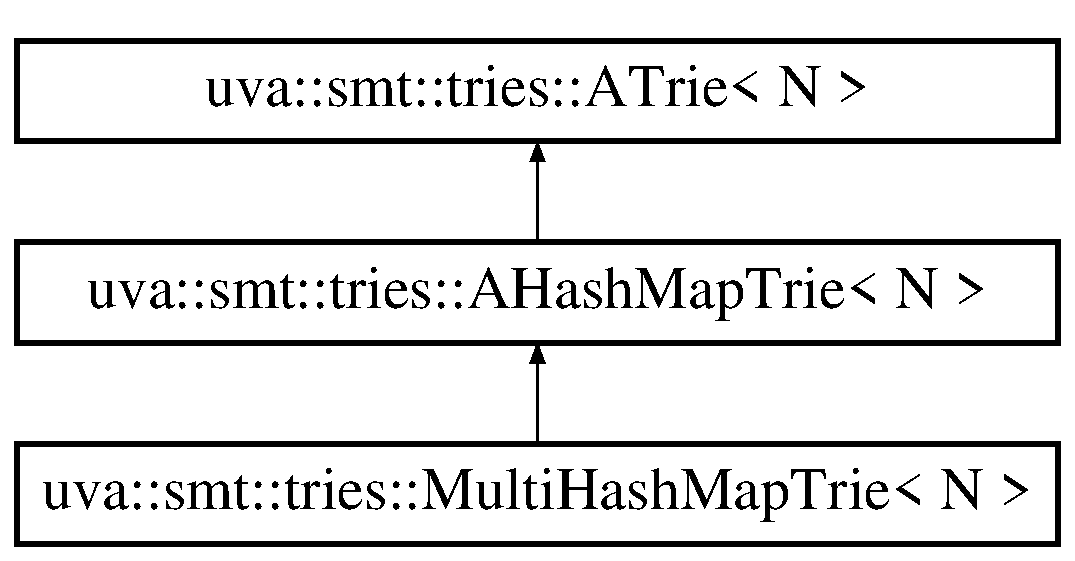
\includegraphics[height=3.000000cm]{classuva_1_1smt_1_1tries_1_1_multi_hash_map_trie}
\end{center}
\end{figure}
\subsection*{Public Member Functions}
\begin{DoxyCompactItemize}
\item 
\hyperlink{classuva_1_1smt_1_1tries_1_1_multi_hash_map_trie_a33184c09e7b63bcdbfad0443492cab93}{Multi\+Hash\+Map\+Trie} (const float word\+Index\+Mem\+Factor)
\item 
virtual void \hyperlink{classuva_1_1smt_1_1tries_1_1_multi_hash_map_trie_ac7d916356f0ad36d33c0c4722e6459b9}{pre\+Allocate} (const size\+\_\+t counts\mbox{[}N\mbox{]})
\item 
virtual void \hyperlink{classuva_1_1smt_1_1tries_1_1_multi_hash_map_trie_aa49f2f0ed0d86038fe5efb13e6ee70a5}{add1\+Gram} (const \hyperlink{structuva_1_1smt_1_1tries_1_1_s_back_off_n_gram}{S\+Back\+Off\+N\+Gram} \&o\+Gram)
\item 
virtual void \hyperlink{classuva_1_1smt_1_1tries_1_1_multi_hash_map_trie_aa01609671de94014323015352e03c441}{add\+M\+Gram} (const \hyperlink{structuva_1_1smt_1_1tries_1_1_s_back_off_n_gram}{S\+Back\+Off\+N\+Gram} \&m\+Gram)
\item 
virtual void \hyperlink{classuva_1_1smt_1_1tries_1_1_multi_hash_map_trie_a3ecb4eb51f5163eedcf100ed8b8f0104}{add\+N\+Gram} (const \hyperlink{structuva_1_1smt_1_1tries_1_1_s_back_off_n_gram}{S\+Back\+Off\+N\+Gram} \&n\+Gram)
\item 
virtual void \hyperlink{classuva_1_1smt_1_1tries_1_1_multi_hash_map_trie_a6b31b10b19c93ea3e6d08923ee1c0df7}{query\+N\+Gram} (const vector$<$ string $>$ \&ngram, \hyperlink{structuva_1_1smt_1_1tries_1_1_s_prob_result}{S\+Prob\+Result} \&result)
\item 
virtual \hyperlink{classuva_1_1smt_1_1tries_1_1_multi_hash_map_trie_aa4b3b06c1768e6a5725e5ff5eda5a6e4}{$\sim$\+Multi\+Hash\+Map\+Trie} ()
\end{DoxyCompactItemize}
\subsection*{Static Public Attributes}
\begin{DoxyCompactItemize}
\item 
static const \hyperlink{namespaceuva_1_1smt_1_1tries_a26064146e98856c7c4185efab0e61a36}{T\+Model\+Level} \hyperlink{classuva_1_1smt_1_1tries_1_1_multi_hash_map_trie_a7efd4616e7d1f51db0cc4cb50f11345e}{M\+G\+R\+A\+M\+\_\+\+I\+D\+X\+\_\+\+O\+F\+F\+S\+E\+T} = 3
\end{DoxyCompactItemize}
\subsection*{Additional Inherited Members}


\subsection{Detailed Description}
\subsubsection*{template$<$T\+Model\+Level N$>$class uva\+::smt\+::tries\+::\+Multi\+Hash\+Map\+Trie$<$ N $>$}

This is a Hash\+Mpa based I\+Trie interface implementation class. Note 1\+: This implementation uses the unsigned long for the hashes it is not optimal Note 2\+: the unordered\+\_\+map might be not as efficient as a hash\+\_\+map with respect to memory usage but it is supposed to be faster

This implementation is chosen because it resembles the ordered array implementation from\+: \char`\"{}\+Faster and Smaller N -\/\+Gram Language Models\char`\"{} Adam Pauls Dan Klein Computer Science Division University of California, Berkeley

and unordered\+\_\+maps showed good performance in\+: \char`\"{}\+Efficient in-\/memory data structures for n-\/grams indexing\char`\"{} Daniel Robenek, Jan Platoˇs, and V ́aclav Sn ́aˇsel Department of Computer Science, F\+E\+I, V\+S\+B – Technical University of Ostrava
\begin{DoxyEnumerate}
\item listopadu 15, 708 33, Ostrava-\/\+Poruba, Czech Republic \{daniel.\+robenek.\+st, jan.\+platos, vaclav.\+snasel\}.cz 
\end{DoxyEnumerate}

\subsection{Constructor \& Destructor Documentation}
\hypertarget{classuva_1_1smt_1_1tries_1_1_multi_hash_map_trie_a33184c09e7b63bcdbfad0443492cab93}{}\index{uva\+::smt\+::tries\+::\+Multi\+Hash\+Map\+Trie@{uva\+::smt\+::tries\+::\+Multi\+Hash\+Map\+Trie}!Multi\+Hash\+Map\+Trie@{Multi\+Hash\+Map\+Trie}}
\index{Multi\+Hash\+Map\+Trie@{Multi\+Hash\+Map\+Trie}!uva\+::smt\+::tries\+::\+Multi\+Hash\+Map\+Trie@{uva\+::smt\+::tries\+::\+Multi\+Hash\+Map\+Trie}}
\subsubsection[{Multi\+Hash\+Map\+Trie(const float word\+Index\+Mem\+Factor)}]{\setlength{\rightskip}{0pt plus 5cm}template$<$T\+Model\+Level N$>$ {\bf uva\+::smt\+::tries\+::\+Multi\+Hash\+Map\+Trie}$<$ N $>$\+::{\bf Multi\+Hash\+Map\+Trie} (
\begin{DoxyParamCaption}
\item[{const float}]{word\+Index\+Mem\+Factor}
\end{DoxyParamCaption}
)\hspace{0.3cm}{\ttfamily [explicit]}}\label{classuva_1_1smt_1_1tries_1_1_multi_hash_map_trie_a33184c09e7b63bcdbfad0443492cab93}
The basic class constructor, accepts memory factor(s) that are the coefficients used when pre-\/allocating memory for unordered maps.

If a factor is equal to 0.\+0 then no memory is pre-\/allocated. If the factor is equal to 1.\+0 then there is only as much preallocated as needed to store the gram entries. The latter is typically not enough as unordered\+\_\+map needs more memory for internal administration. If there is not enough memory pre-\/allocated then additional allocations will take place but it does not alway lead to more efficient memory usage. The observed behavior is that it is better to pre-\/allocate a bit more memory beforehand, than needed. This leads to less memory consumption. Depending on the type of unordered\+\_\+map key/value pair types the advised factor values are from 2.\+0 to 2.\+6. Because it can not be optimally determined beforehand, these are made constructor parameters so that they can be configured by the used. This breaks encapsulation a bit, exposing the internals, but there is no other better way, for fine tuning the memory usage.


\begin{DoxyParams}{Parameters}
{\em word\+Index\+Mem\+Factor} & the assigned memory factor for storage allocation in the unordered\+\_\+map used for the word index \\
\hline
\end{DoxyParams}
\hypertarget{classuva_1_1smt_1_1tries_1_1_multi_hash_map_trie_aa4b3b06c1768e6a5725e5ff5eda5a6e4}{}\index{uva\+::smt\+::tries\+::\+Multi\+Hash\+Map\+Trie@{uva\+::smt\+::tries\+::\+Multi\+Hash\+Map\+Trie}!````~Multi\+Hash\+Map\+Trie@{$\sim$\+Multi\+Hash\+Map\+Trie}}
\index{````~Multi\+Hash\+Map\+Trie@{$\sim$\+Multi\+Hash\+Map\+Trie}!uva\+::smt\+::tries\+::\+Multi\+Hash\+Map\+Trie@{uva\+::smt\+::tries\+::\+Multi\+Hash\+Map\+Trie}}
\subsubsection[{$\sim$\+Multi\+Hash\+Map\+Trie()}]{\setlength{\rightskip}{0pt plus 5cm}template$<$T\+Model\+Level N$>$ virtual {\bf uva\+::smt\+::tries\+::\+Multi\+Hash\+Map\+Trie}$<$ N $>$\+::$\sim${\bf Multi\+Hash\+Map\+Trie} (
\begin{DoxyParamCaption}
{}
\end{DoxyParamCaption}
)\hspace{0.3cm}{\ttfamily [inline]}, {\ttfamily [virtual]}}\label{classuva_1_1smt_1_1tries_1_1_multi_hash_map_trie_aa4b3b06c1768e6a5725e5ff5eda5a6e4}
The destructor 

\subsection{Member Function Documentation}
\hypertarget{classuva_1_1smt_1_1tries_1_1_multi_hash_map_trie_aa49f2f0ed0d86038fe5efb13e6ee70a5}{}\index{uva\+::smt\+::tries\+::\+Multi\+Hash\+Map\+Trie@{uva\+::smt\+::tries\+::\+Multi\+Hash\+Map\+Trie}!add1\+Gram@{add1\+Gram}}
\index{add1\+Gram@{add1\+Gram}!uva\+::smt\+::tries\+::\+Multi\+Hash\+Map\+Trie@{uva\+::smt\+::tries\+::\+Multi\+Hash\+Map\+Trie}}
\subsubsection[{add1\+Gram(const S\+Back\+Off\+N\+Gram \&o\+Gram)}]{\setlength{\rightskip}{0pt plus 5cm}template$<$T\+Model\+Level N$>$ void {\bf uva\+::smt\+::tries\+::\+Multi\+Hash\+Map\+Trie}$<$ N $>$\+::add1\+Gram (
\begin{DoxyParamCaption}
\item[{const {\bf S\+Back\+Off\+N\+Gram} \&}]{o\+Gram}
\end{DoxyParamCaption}
)\hspace{0.3cm}{\ttfamily [virtual]}}\label{classuva_1_1smt_1_1tries_1_1_multi_hash_map_trie_aa49f2f0ed0d86038fe5efb13e6ee70a5}
This method adds a 1-\/\+Gram (word) to the trie. For more details \begin{DoxySeeAlso}{See also}
I\+Trie 
\end{DoxySeeAlso}


Implements \hyperlink{classuva_1_1smt_1_1tries_1_1_a_trie_af184dbb0b095d24c76f79c7da6479eda}{uva\+::smt\+::tries\+::\+A\+Trie$<$ N $>$}.

\hypertarget{classuva_1_1smt_1_1tries_1_1_multi_hash_map_trie_aa01609671de94014323015352e03c441}{}\index{uva\+::smt\+::tries\+::\+Multi\+Hash\+Map\+Trie@{uva\+::smt\+::tries\+::\+Multi\+Hash\+Map\+Trie}!add\+M\+Gram@{add\+M\+Gram}}
\index{add\+M\+Gram@{add\+M\+Gram}!uva\+::smt\+::tries\+::\+Multi\+Hash\+Map\+Trie@{uva\+::smt\+::tries\+::\+Multi\+Hash\+Map\+Trie}}
\subsubsection[{add\+M\+Gram(const S\+Back\+Off\+N\+Gram \&m\+Gram)}]{\setlength{\rightskip}{0pt plus 5cm}template$<$T\+Model\+Level N$>$ void {\bf uva\+::smt\+::tries\+::\+Multi\+Hash\+Map\+Trie}$<$ N $>$\+::add\+M\+Gram (
\begin{DoxyParamCaption}
\item[{const {\bf S\+Back\+Off\+N\+Gram} \&}]{m\+Gram}
\end{DoxyParamCaption}
)\hspace{0.3cm}{\ttfamily [virtual]}}\label{classuva_1_1smt_1_1tries_1_1_multi_hash_map_trie_aa01609671de94014323015352e03c441}
This method adds a M-\/\+Gram (word) to the trie where 1 $<$ M $<$ N For more details \begin{DoxySeeAlso}{See also}
I\+Trie 
\end{DoxySeeAlso}


Implements \hyperlink{classuva_1_1smt_1_1tries_1_1_a_trie_acf62fc322ece5ec01ca00e96e17eb9ef}{uva\+::smt\+::tries\+::\+A\+Trie$<$ N $>$}.

\hypertarget{classuva_1_1smt_1_1tries_1_1_multi_hash_map_trie_a3ecb4eb51f5163eedcf100ed8b8f0104}{}\index{uva\+::smt\+::tries\+::\+Multi\+Hash\+Map\+Trie@{uva\+::smt\+::tries\+::\+Multi\+Hash\+Map\+Trie}!add\+N\+Gram@{add\+N\+Gram}}
\index{add\+N\+Gram@{add\+N\+Gram}!uva\+::smt\+::tries\+::\+Multi\+Hash\+Map\+Trie@{uva\+::smt\+::tries\+::\+Multi\+Hash\+Map\+Trie}}
\subsubsection[{add\+N\+Gram(const S\+Back\+Off\+N\+Gram \&n\+Gram)}]{\setlength{\rightskip}{0pt plus 5cm}template$<$T\+Model\+Level N$>$ void {\bf uva\+::smt\+::tries\+::\+Multi\+Hash\+Map\+Trie}$<$ N $>$\+::add\+N\+Gram (
\begin{DoxyParamCaption}
\item[{const {\bf S\+Back\+Off\+N\+Gram} \&}]{n\+Gram}
\end{DoxyParamCaption}
)\hspace{0.3cm}{\ttfamily [virtual]}}\label{classuva_1_1smt_1_1tries_1_1_multi_hash_map_trie_a3ecb4eb51f5163eedcf100ed8b8f0104}
This method adds a N-\/\+Gram (word) to the trie where For more details \begin{DoxySeeAlso}{See also}
I\+Trie 
\end{DoxySeeAlso}


Implements \hyperlink{classuva_1_1smt_1_1tries_1_1_a_trie_a240c090a5651e74304cf37b131ca9741}{uva\+::smt\+::tries\+::\+A\+Trie$<$ N $>$}.

\hypertarget{classuva_1_1smt_1_1tries_1_1_multi_hash_map_trie_ac7d916356f0ad36d33c0c4722e6459b9}{}\index{uva\+::smt\+::tries\+::\+Multi\+Hash\+Map\+Trie@{uva\+::smt\+::tries\+::\+Multi\+Hash\+Map\+Trie}!pre\+Allocate@{pre\+Allocate}}
\index{pre\+Allocate@{pre\+Allocate}!uva\+::smt\+::tries\+::\+Multi\+Hash\+Map\+Trie@{uva\+::smt\+::tries\+::\+Multi\+Hash\+Map\+Trie}}
\subsubsection[{pre\+Allocate(const size\+\_\+t counts[N])}]{\setlength{\rightskip}{0pt plus 5cm}template$<$T\+Model\+Level N$>$ void {\bf uva\+::smt\+::tries\+::\+Multi\+Hash\+Map\+Trie}$<$ N $>$\+::pre\+Allocate (
\begin{DoxyParamCaption}
\item[{const size\+\_\+t}]{counts\mbox{[}\+N\mbox{]}}
\end{DoxyParamCaption}
)\hspace{0.3cm}{\ttfamily [virtual]}}\label{classuva_1_1smt_1_1tries_1_1_multi_hash_map_trie_ac7d916356f0ad36d33c0c4722e6459b9}
This method can be used to provide the N-\/gram count information That should allow for pre-\/allocation of the memory For more details \begin{DoxySeeAlso}{See also}
I\+Trie 
\end{DoxySeeAlso}


Reimplemented from \hyperlink{classuva_1_1smt_1_1tries_1_1_a_hash_map_trie_ad867b72350326f464b563fba6727ba5f}{uva\+::smt\+::tries\+::\+A\+Hash\+Map\+Trie$<$ N $>$}.

\hypertarget{classuva_1_1smt_1_1tries_1_1_multi_hash_map_trie_a6b31b10b19c93ea3e6d08923ee1c0df7}{}\index{uva\+::smt\+::tries\+::\+Multi\+Hash\+Map\+Trie@{uva\+::smt\+::tries\+::\+Multi\+Hash\+Map\+Trie}!query\+N\+Gram@{query\+N\+Gram}}
\index{query\+N\+Gram@{query\+N\+Gram}!uva\+::smt\+::tries\+::\+Multi\+Hash\+Map\+Trie@{uva\+::smt\+::tries\+::\+Multi\+Hash\+Map\+Trie}}
\subsubsection[{query\+N\+Gram(const vector$<$ string $>$ \&ngram, S\+Prob\+Result \&result)}]{\setlength{\rightskip}{0pt plus 5cm}template$<$T\+Model\+Level N$>$ void {\bf uva\+::smt\+::tries\+::\+Multi\+Hash\+Map\+Trie}$<$ N $>$\+::query\+N\+Gram (
\begin{DoxyParamCaption}
\item[{const vector$<$ string $>$ \&}]{ngram, }
\item[{{\bf S\+Prob\+Result} \&}]{result}
\end{DoxyParamCaption}
)\hspace{0.3cm}{\ttfamily [virtual]}}\label{classuva_1_1smt_1_1tries_1_1_multi_hash_map_trie_a6b31b10b19c93ea3e6d08923ee1c0df7}
This method will get the N-\/gram in a form of a vector, e.\+g.\+: \mbox{[}word1 word2 word3 word4 word5\mbox{]} and will compute and return the Language Model Probability for it For more details \begin{DoxySeeAlso}{See also}
I\+Trie 
\end{DoxySeeAlso}


Implements \hyperlink{classuva_1_1smt_1_1tries_1_1_a_trie_a86f8301bb7a9e7a232f16bcd000062b2}{uva\+::smt\+::tries\+::\+A\+Trie$<$ N $>$}.



\subsection{Member Data Documentation}
\hypertarget{classuva_1_1smt_1_1tries_1_1_multi_hash_map_trie_a7efd4616e7d1f51db0cc4cb50f11345e}{}\index{uva\+::smt\+::tries\+::\+Multi\+Hash\+Map\+Trie@{uva\+::smt\+::tries\+::\+Multi\+Hash\+Map\+Trie}!M\+G\+R\+A\+M\+\_\+\+I\+D\+X\+\_\+\+O\+F\+F\+S\+E\+T@{M\+G\+R\+A\+M\+\_\+\+I\+D\+X\+\_\+\+O\+F\+F\+S\+E\+T}}
\index{M\+G\+R\+A\+M\+\_\+\+I\+D\+X\+\_\+\+O\+F\+F\+S\+E\+T@{M\+G\+R\+A\+M\+\_\+\+I\+D\+X\+\_\+\+O\+F\+F\+S\+E\+T}!uva\+::smt\+::tries\+::\+Multi\+Hash\+Map\+Trie@{uva\+::smt\+::tries\+::\+Multi\+Hash\+Map\+Trie}}
\subsubsection[{M\+G\+R\+A\+M\+\_\+\+I\+D\+X\+\_\+\+O\+F\+F\+S\+E\+T}]{\setlength{\rightskip}{0pt plus 5cm}template$<$T\+Model\+Level N$>$ const {\bf T\+Model\+Level} {\bf uva\+::smt\+::tries\+::\+Multi\+Hash\+Map\+Trie}$<$ N $>$\+::M\+G\+R\+A\+M\+\_\+\+I\+D\+X\+\_\+\+O\+F\+F\+S\+E\+T = 3\hspace{0.3cm}{\ttfamily [static]}}\label{classuva_1_1smt_1_1tries_1_1_multi_hash_map_trie_a7efd4616e7d1f51db0cc4cb50f11345e}


The documentation for this class was generated from the following files\+:\begin{DoxyCompactItemize}
\item 
inc/\hyperlink{_multi_hash_map_trie_8hpp}{Multi\+Hash\+Map\+Trie.\+hpp}\item 
src/\hyperlink{_multi_hash_map_trie_8cpp}{Multi\+Hash\+Map\+Trie.\+cpp}\end{DoxyCompactItemize}

\hypertarget{structuva_1_1smt_1_1tries_1_1alloc_1_1_greedy_memory_allocator_1_1rebind}{}\section{uva\+:\+:smt\+:\+:tries\+:\+:alloc\+:\+:Greedy\+Memory\+Allocator$<$ T $>$\+:\+:rebind$<$ U $>$ Struct Template Reference}
\label{structuva_1_1smt_1_1tries_1_1alloc_1_1_greedy_memory_allocator_1_1rebind}\index{uva\+::smt\+::tries\+::alloc\+::\+Greedy\+Memory\+Allocator$<$ T $>$\+::rebind$<$ U $>$@{uva\+::smt\+::tries\+::alloc\+::\+Greedy\+Memory\+Allocator$<$ T $>$\+::rebind$<$ U $>$}}


{\ttfamily \#include $<$Greedy\+Memory\+Allocator.\+hpp$>$}

\subsection*{Public Types}
\begin{DoxyCompactItemize}
\item 
typedef \hyperlink{classuva_1_1smt_1_1tries_1_1alloc_1_1_greedy_memory_allocator}{Greedy\+Memory\+Allocator}$<$ U $>$ \hyperlink{structuva_1_1smt_1_1tries_1_1alloc_1_1_greedy_memory_allocator_1_1rebind_a4c9a2812bdf3606f7e8a1cbe635fea90}{other}
\end{DoxyCompactItemize}


\subsection{Member Typedef Documentation}
\hypertarget{structuva_1_1smt_1_1tries_1_1alloc_1_1_greedy_memory_allocator_1_1rebind_a4c9a2812bdf3606f7e8a1cbe635fea90}{}\index{uva\+::smt\+::tries\+::alloc\+::\+Greedy\+Memory\+Allocator\+::rebind@{uva\+::smt\+::tries\+::alloc\+::\+Greedy\+Memory\+Allocator\+::rebind}!other@{other}}
\index{other@{other}!uva\+::smt\+::tries\+::alloc\+::\+Greedy\+Memory\+Allocator\+::rebind@{uva\+::smt\+::tries\+::alloc\+::\+Greedy\+Memory\+Allocator\+::rebind}}
\subsubsection[{other}]{\setlength{\rightskip}{0pt plus 5cm}template$<$typename T$>$ template$<$typename U $>$ typedef {\bf Greedy\+Memory\+Allocator}$<$U$>$ {\bf uva\+::smt\+::tries\+::alloc\+::\+Greedy\+Memory\+Allocator}$<$ T $>$\+::{\bf rebind}$<$ U $>$\+::{\bf other}}\label{structuva_1_1smt_1_1tries_1_1alloc_1_1_greedy_memory_allocator_1_1rebind_a4c9a2812bdf3606f7e8a1cbe635fea90}


The documentation for this struct was generated from the following file\+:\begin{DoxyCompactItemize}
\item 
inc/\hyperlink{_greedy_memory_allocator_8hpp}{Greedy\+Memory\+Allocator.\+hpp}\end{DoxyCompactItemize}

\hypertarget{structuva_1_1smt_1_1tries_1_1_s_back_off_n_gram}{}\section{uva\+:\+:smt\+:\+:tries\+:\+:S\+Back\+Off\+N\+Gram Struct Reference}
\label{structuva_1_1smt_1_1tries_1_1_s_back_off_n_gram}\index{uva\+::smt\+::tries\+::\+S\+Back\+Off\+N\+Gram@{uva\+::smt\+::tries\+::\+S\+Back\+Off\+N\+Gram}}


{\ttfamily \#include $<$A\+Trie.\+hpp$>$}

\subsection*{Public Attributes}
\begin{DoxyCompactItemize}
\item 
\hyperlink{namespaceuva_1_1smt_1_1tries_acd0660255dd9ef5d644f01de49102750}{T\+Log\+Prob\+Back\+Off} \hyperlink{structuva_1_1smt_1_1tries_1_1_s_back_off_n_gram_a3af5b26367189b16778ff72a5cd29abc}{prob}
\item 
\hyperlink{namespaceuva_1_1smt_1_1tries_acd0660255dd9ef5d644f01de49102750}{T\+Log\+Prob\+Back\+Off} \hyperlink{structuva_1_1smt_1_1tries_1_1_s_back_off_n_gram_ae299498d72b31a024af702332ff6a49c}{back\+\_\+off}
\item 
vector$<$ string $>$ \hyperlink{structuva_1_1smt_1_1tries_1_1_s_back_off_n_gram_ab862f62269c845d2587dfcb7b9491271}{tokens}
\end{DoxyCompactItemize}


\subsection{Detailed Description}
This structure is used to store the N-\/\+Gram data of the back-\/off Language Model. 
\begin{DoxyParams}{Parameters}
{\em prob} & stores the log\+\_\+10 probability of the N-\/\+Gram Must be a negative value \\
\hline
{\em back\+\_\+off} & stores the log\+\_\+10 back-\/off weight (probability) of the N-\/gram can be 0 is the probability is not available \\
\hline
{\em tokens} & stores the N-\/gram words the size of this vector defines the N-\/gram level. \\
\hline
\end{DoxyParams}


\subsection{Member Data Documentation}
\hypertarget{structuva_1_1smt_1_1tries_1_1_s_back_off_n_gram_ae299498d72b31a024af702332ff6a49c}{}\index{uva\+::smt\+::tries\+::\+S\+Back\+Off\+N\+Gram@{uva\+::smt\+::tries\+::\+S\+Back\+Off\+N\+Gram}!back\+\_\+off@{back\+\_\+off}}
\index{back\+\_\+off@{back\+\_\+off}!uva\+::smt\+::tries\+::\+S\+Back\+Off\+N\+Gram@{uva\+::smt\+::tries\+::\+S\+Back\+Off\+N\+Gram}}
\subsubsection[{back\+\_\+off}]{\setlength{\rightskip}{0pt plus 5cm}{\bf T\+Log\+Prob\+Back\+Off} uva\+::smt\+::tries\+::\+S\+Back\+Off\+N\+Gram\+::back\+\_\+off}\label{structuva_1_1smt_1_1tries_1_1_s_back_off_n_gram_ae299498d72b31a024af702332ff6a49c}
\hypertarget{structuva_1_1smt_1_1tries_1_1_s_back_off_n_gram_a3af5b26367189b16778ff72a5cd29abc}{}\index{uva\+::smt\+::tries\+::\+S\+Back\+Off\+N\+Gram@{uva\+::smt\+::tries\+::\+S\+Back\+Off\+N\+Gram}!prob@{prob}}
\index{prob@{prob}!uva\+::smt\+::tries\+::\+S\+Back\+Off\+N\+Gram@{uva\+::smt\+::tries\+::\+S\+Back\+Off\+N\+Gram}}
\subsubsection[{prob}]{\setlength{\rightskip}{0pt plus 5cm}{\bf T\+Log\+Prob\+Back\+Off} uva\+::smt\+::tries\+::\+S\+Back\+Off\+N\+Gram\+::prob}\label{structuva_1_1smt_1_1tries_1_1_s_back_off_n_gram_a3af5b26367189b16778ff72a5cd29abc}
\hypertarget{structuva_1_1smt_1_1tries_1_1_s_back_off_n_gram_ab862f62269c845d2587dfcb7b9491271}{}\index{uva\+::smt\+::tries\+::\+S\+Back\+Off\+N\+Gram@{uva\+::smt\+::tries\+::\+S\+Back\+Off\+N\+Gram}!tokens@{tokens}}
\index{tokens@{tokens}!uva\+::smt\+::tries\+::\+S\+Back\+Off\+N\+Gram@{uva\+::smt\+::tries\+::\+S\+Back\+Off\+N\+Gram}}
\subsubsection[{tokens}]{\setlength{\rightskip}{0pt plus 5cm}vector$<$string$>$ uva\+::smt\+::tries\+::\+S\+Back\+Off\+N\+Gram\+::tokens}\label{structuva_1_1smt_1_1tries_1_1_s_back_off_n_gram_ab862f62269c845d2587dfcb7b9491271}


The documentation for this struct was generated from the following file\+:\begin{DoxyCompactItemize}
\item 
inc/\hyperlink{_a_trie_8hpp}{A\+Trie.\+hpp}\end{DoxyCompactItemize}

\hypertarget{classuva_1_1smt_1_1tries_1_1_single_hash_map_trie}{}\section{uva\+:\+:smt\+:\+:tries\+:\+:Single\+Hash\+Map\+Trie$<$ N $>$ Class Template Reference}
\label{classuva_1_1smt_1_1tries_1_1_single_hash_map_trie}\index{uva\+::smt\+::tries\+::\+Single\+Hash\+Map\+Trie$<$ N $>$@{uva\+::smt\+::tries\+::\+Single\+Hash\+Map\+Trie$<$ N $>$}}


{\ttfamily \#include $<$Single\+Hash\+Map\+Trie.\+hpp$>$}

Inheritance diagram for uva\+:\+:smt\+:\+:tries\+:\+:Single\+Hash\+Map\+Trie$<$ N $>$\+:\begin{figure}[H]
\begin{center}
\leavevmode
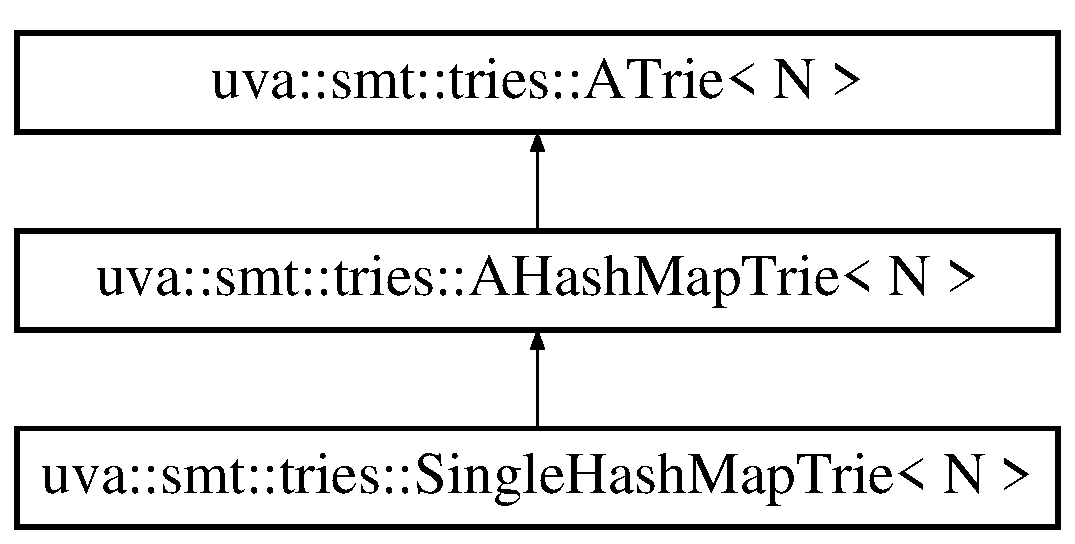
\includegraphics[height=3.000000cm]{classuva_1_1smt_1_1tries_1_1_single_hash_map_trie}
\end{center}
\end{figure}
\subsection*{Public Member Functions}
\begin{DoxyCompactItemize}
\item 
\hyperlink{classuva_1_1smt_1_1tries_1_1_single_hash_map_trie_aeb7a9f63ac580aa6004c6e041cfae4a7}{Single\+Hash\+Map\+Trie} (const float word\+Index\+Mem\+Factor)
\item 
virtual void \hyperlink{classuva_1_1smt_1_1tries_1_1_single_hash_map_trie_a6a40f4047280dedc7f402d6502547b2c}{pre\+Allocate} (const size\+\_\+t counts\mbox{[}N\mbox{]})
\item 
virtual void \hyperlink{classuva_1_1smt_1_1tries_1_1_single_hash_map_trie_a27f420ad02db97ab648ef27ffb12e688}{add1\+Gram} (const \hyperlink{structuva_1_1smt_1_1tries_1_1_s_back_off_n_gram}{S\+Back\+Off\+N\+Gram} \&o\+Gram)
\item 
virtual void \hyperlink{classuva_1_1smt_1_1tries_1_1_single_hash_map_trie_a2da8d1cba4cdbab7cc79bcfc4f55117b}{add\+M\+Gram} (const \hyperlink{structuva_1_1smt_1_1tries_1_1_s_back_off_n_gram}{S\+Back\+Off\+N\+Gram} \&m\+Gram)
\item 
virtual void \hyperlink{classuva_1_1smt_1_1tries_1_1_single_hash_map_trie_af9541116f44c985e80f9d1173512fc4f}{add\+N\+Gram} (const \hyperlink{structuva_1_1smt_1_1tries_1_1_s_back_off_n_gram}{S\+Back\+Off\+N\+Gram} \&n\+Gram)
\item 
virtual void \hyperlink{classuva_1_1smt_1_1tries_1_1_single_hash_map_trie_ac0a2b8c57ccfd60a8b06ea2116cf8349}{query\+N\+Gram} (const vector$<$ string $>$ \&ngram, \hyperlink{structuva_1_1smt_1_1tries_1_1_s_prob_result}{S\+Prob\+Result} \&result)
\item 
virtual \hyperlink{classuva_1_1smt_1_1tries_1_1_single_hash_map_trie_aac6973244c2fc6cdfac3d2200c4b9dcf}{$\sim$\+Single\+Hash\+Map\+Trie} ()
\end{DoxyCompactItemize}
\subsection*{Additional Inherited Members}


\subsection{Detailed Description}
\subsubsection*{template$<$T\+Model\+Level N$>$class uva\+::smt\+::tries\+::\+Single\+Hash\+Map\+Trie$<$ N $>$}

This is a Hash\+Mpa based I\+Trie interface implementation class.

This implementation is chosen because it resembles the single hashmap implementation mentioned in\+: \char`\"{}\+Ken\+L\+M\+: Faster and Smaller Language Model Queries\char`\"{} Kenneth Heafield Carnegie Mellon University 5000 Forbes Ave Pittsburgh, P\+A 15213 U\+S\+A \href{mailto:heafield@cs.cmu.edu}{\tt heafield@cs.\+cmu.\+edu}

and unordered\+\_\+maps showed good performance in\+: \char`\"{}\+Efficient in-\/memory data structures for n-\/grams indexing\char`\"{} Daniel Robenek, Jan Platoˇs, and V ́aclav Sn ́aˇsel Department of Computer Science, F\+E\+I, V\+S\+B – Technical University of Ostrava
\begin{DoxyEnumerate}
\item listopadu 15, 708 33, Ostrava-\/\+Poruba, Czech Republic \{daniel.\+robenek.\+st, jan.\+platos, vaclav.\+snasel\}.cz 
\end{DoxyEnumerate}

\subsection{Constructor \& Destructor Documentation}
\hypertarget{classuva_1_1smt_1_1tries_1_1_single_hash_map_trie_aeb7a9f63ac580aa6004c6e041cfae4a7}{}\index{uva\+::smt\+::tries\+::\+Single\+Hash\+Map\+Trie@{uva\+::smt\+::tries\+::\+Single\+Hash\+Map\+Trie}!Single\+Hash\+Map\+Trie@{Single\+Hash\+Map\+Trie}}
\index{Single\+Hash\+Map\+Trie@{Single\+Hash\+Map\+Trie}!uva\+::smt\+::tries\+::\+Single\+Hash\+Map\+Trie@{uva\+::smt\+::tries\+::\+Single\+Hash\+Map\+Trie}}
\subsubsection[{Single\+Hash\+Map\+Trie(const float word\+Index\+Mem\+Factor)}]{\setlength{\rightskip}{0pt plus 5cm}template$<$T\+Model\+Level N$>$ {\bf uva\+::smt\+::tries\+::\+Single\+Hash\+Map\+Trie}$<$ N $>$\+::{\bf Single\+Hash\+Map\+Trie} (
\begin{DoxyParamCaption}
\item[{const float}]{word\+Index\+Mem\+Factor}
\end{DoxyParamCaption}
)\hspace{0.3cm}{\ttfamily [explicit]}}\label{classuva_1_1smt_1_1tries_1_1_single_hash_map_trie_aeb7a9f63ac580aa6004c6e041cfae4a7}
The basic class constructor, accepts memory factor(s) that are the coefficients used when pre-\/allocating memory for unordered maps.

If a factor is equal to 0.\+0 then no memory is pre-\/allocated. If the factor is equal to 1.\+0 then there is only as much preallocated as needed to store the gram entries. The latter is typically not enough as unordered\+\_\+map needs more memory for internal administration. If there is not enough memory pre-\/allocated then additional allocations will take place but it does not alway lead to more efficient memory usage. The observed behavior is that it is better to pre-\/allocate a bit more memory beforehand, than needed. This leads to less memory consumption. Depending on the type of unordered\+\_\+map key/value pair types the advised factor values are from 2.\+0 to 2.\+6. Because it can not be optimally determined beforehand, these are made constructor parameters so that they can be configured by the used. This breaks encapsulation a bit, exposing the internals, but there is no other better way, for fine tuning the memory usage.


\begin{DoxyParams}{Parameters}
{\em word\+Index\+Mem\+Factor} & the assigned memory factor for storage allocation in the unordered\+\_\+map used for the word index \\
\hline
\end{DoxyParams}
\hypertarget{classuva_1_1smt_1_1tries_1_1_single_hash_map_trie_aac6973244c2fc6cdfac3d2200c4b9dcf}{}\index{uva\+::smt\+::tries\+::\+Single\+Hash\+Map\+Trie@{uva\+::smt\+::tries\+::\+Single\+Hash\+Map\+Trie}!````~Single\+Hash\+Map\+Trie@{$\sim$\+Single\+Hash\+Map\+Trie}}
\index{````~Single\+Hash\+Map\+Trie@{$\sim$\+Single\+Hash\+Map\+Trie}!uva\+::smt\+::tries\+::\+Single\+Hash\+Map\+Trie@{uva\+::smt\+::tries\+::\+Single\+Hash\+Map\+Trie}}
\subsubsection[{$\sim$\+Single\+Hash\+Map\+Trie()}]{\setlength{\rightskip}{0pt plus 5cm}template$<$T\+Model\+Level N$>$ virtual {\bf uva\+::smt\+::tries\+::\+Single\+Hash\+Map\+Trie}$<$ N $>$\+::$\sim${\bf Single\+Hash\+Map\+Trie} (
\begin{DoxyParamCaption}
{}
\end{DoxyParamCaption}
)\hspace{0.3cm}{\ttfamily [inline]}, {\ttfamily [virtual]}}\label{classuva_1_1smt_1_1tries_1_1_single_hash_map_trie_aac6973244c2fc6cdfac3d2200c4b9dcf}
The destructor 

\subsection{Member Function Documentation}
\hypertarget{classuva_1_1smt_1_1tries_1_1_single_hash_map_trie_a27f420ad02db97ab648ef27ffb12e688}{}\index{uva\+::smt\+::tries\+::\+Single\+Hash\+Map\+Trie@{uva\+::smt\+::tries\+::\+Single\+Hash\+Map\+Trie}!add1\+Gram@{add1\+Gram}}
\index{add1\+Gram@{add1\+Gram}!uva\+::smt\+::tries\+::\+Single\+Hash\+Map\+Trie@{uva\+::smt\+::tries\+::\+Single\+Hash\+Map\+Trie}}
\subsubsection[{add1\+Gram(const S\+Back\+Off\+N\+Gram \&o\+Gram)}]{\setlength{\rightskip}{0pt plus 5cm}template$<$T\+Model\+Level N$>$ void {\bf uva\+::smt\+::tries\+::\+Single\+Hash\+Map\+Trie}$<$ N $>$\+::add1\+Gram (
\begin{DoxyParamCaption}
\item[{const {\bf S\+Back\+Off\+N\+Gram} \&}]{o\+Gram}
\end{DoxyParamCaption}
)\hspace{0.3cm}{\ttfamily [virtual]}}\label{classuva_1_1smt_1_1tries_1_1_single_hash_map_trie_a27f420ad02db97ab648ef27ffb12e688}
This method adds a 1-\/\+Gram (word) to the trie. For more details \begin{DoxySeeAlso}{See also}
I\+Trie 
\end{DoxySeeAlso}


Implements \hyperlink{classuva_1_1smt_1_1tries_1_1_a_trie_af184dbb0b095d24c76f79c7da6479eda}{uva\+::smt\+::tries\+::\+A\+Trie$<$ N $>$}.

\hypertarget{classuva_1_1smt_1_1tries_1_1_single_hash_map_trie_a2da8d1cba4cdbab7cc79bcfc4f55117b}{}\index{uva\+::smt\+::tries\+::\+Single\+Hash\+Map\+Trie@{uva\+::smt\+::tries\+::\+Single\+Hash\+Map\+Trie}!add\+M\+Gram@{add\+M\+Gram}}
\index{add\+M\+Gram@{add\+M\+Gram}!uva\+::smt\+::tries\+::\+Single\+Hash\+Map\+Trie@{uva\+::smt\+::tries\+::\+Single\+Hash\+Map\+Trie}}
\subsubsection[{add\+M\+Gram(const S\+Back\+Off\+N\+Gram \&m\+Gram)}]{\setlength{\rightskip}{0pt plus 5cm}template$<$T\+Model\+Level N$>$ void {\bf uva\+::smt\+::tries\+::\+Single\+Hash\+Map\+Trie}$<$ N $>$\+::add\+M\+Gram (
\begin{DoxyParamCaption}
\item[{const {\bf S\+Back\+Off\+N\+Gram} \&}]{m\+Gram}
\end{DoxyParamCaption}
)\hspace{0.3cm}{\ttfamily [virtual]}}\label{classuva_1_1smt_1_1tries_1_1_single_hash_map_trie_a2da8d1cba4cdbab7cc79bcfc4f55117b}
This method adds a M-\/\+Gram (word) to the trie where 1 $<$ M $<$ N For more details \begin{DoxySeeAlso}{See also}
I\+Trie 
\end{DoxySeeAlso}


Implements \hyperlink{classuva_1_1smt_1_1tries_1_1_a_trie_acf62fc322ece5ec01ca00e96e17eb9ef}{uva\+::smt\+::tries\+::\+A\+Trie$<$ N $>$}.

\hypertarget{classuva_1_1smt_1_1tries_1_1_single_hash_map_trie_af9541116f44c985e80f9d1173512fc4f}{}\index{uva\+::smt\+::tries\+::\+Single\+Hash\+Map\+Trie@{uva\+::smt\+::tries\+::\+Single\+Hash\+Map\+Trie}!add\+N\+Gram@{add\+N\+Gram}}
\index{add\+N\+Gram@{add\+N\+Gram}!uva\+::smt\+::tries\+::\+Single\+Hash\+Map\+Trie@{uva\+::smt\+::tries\+::\+Single\+Hash\+Map\+Trie}}
\subsubsection[{add\+N\+Gram(const S\+Back\+Off\+N\+Gram \&n\+Gram)}]{\setlength{\rightskip}{0pt plus 5cm}template$<$T\+Model\+Level N$>$ void {\bf uva\+::smt\+::tries\+::\+Single\+Hash\+Map\+Trie}$<$ N $>$\+::add\+N\+Gram (
\begin{DoxyParamCaption}
\item[{const {\bf S\+Back\+Off\+N\+Gram} \&}]{n\+Gram}
\end{DoxyParamCaption}
)\hspace{0.3cm}{\ttfamily [virtual]}}\label{classuva_1_1smt_1_1tries_1_1_single_hash_map_trie_af9541116f44c985e80f9d1173512fc4f}
This method adds a N-\/\+Gram (word) to the trie where For more details \begin{DoxySeeAlso}{See also}
I\+Trie 
\end{DoxySeeAlso}


Implements \hyperlink{classuva_1_1smt_1_1tries_1_1_a_trie_a240c090a5651e74304cf37b131ca9741}{uva\+::smt\+::tries\+::\+A\+Trie$<$ N $>$}.

\hypertarget{classuva_1_1smt_1_1tries_1_1_single_hash_map_trie_a6a40f4047280dedc7f402d6502547b2c}{}\index{uva\+::smt\+::tries\+::\+Single\+Hash\+Map\+Trie@{uva\+::smt\+::tries\+::\+Single\+Hash\+Map\+Trie}!pre\+Allocate@{pre\+Allocate}}
\index{pre\+Allocate@{pre\+Allocate}!uva\+::smt\+::tries\+::\+Single\+Hash\+Map\+Trie@{uva\+::smt\+::tries\+::\+Single\+Hash\+Map\+Trie}}
\subsubsection[{pre\+Allocate(const size\+\_\+t counts[N])}]{\setlength{\rightskip}{0pt plus 5cm}template$<$T\+Model\+Level N$>$ void {\bf uva\+::smt\+::tries\+::\+Single\+Hash\+Map\+Trie}$<$ N $>$\+::pre\+Allocate (
\begin{DoxyParamCaption}
\item[{const size\+\_\+t}]{counts\mbox{[}\+N\mbox{]}}
\end{DoxyParamCaption}
)\hspace{0.3cm}{\ttfamily [virtual]}}\label{classuva_1_1smt_1_1tries_1_1_single_hash_map_trie_a6a40f4047280dedc7f402d6502547b2c}
This method can be used to provide the N-\/gram count information That should allow for pre-\/allocation of the memory For more details \begin{DoxySeeAlso}{See also}
I\+Trie 
\end{DoxySeeAlso}


Reimplemented from \hyperlink{classuva_1_1smt_1_1tries_1_1_a_hash_map_trie_ad867b72350326f464b563fba6727ba5f}{uva\+::smt\+::tries\+::\+A\+Hash\+Map\+Trie$<$ N $>$}.

\hypertarget{classuva_1_1smt_1_1tries_1_1_single_hash_map_trie_ac0a2b8c57ccfd60a8b06ea2116cf8349}{}\index{uva\+::smt\+::tries\+::\+Single\+Hash\+Map\+Trie@{uva\+::smt\+::tries\+::\+Single\+Hash\+Map\+Trie}!query\+N\+Gram@{query\+N\+Gram}}
\index{query\+N\+Gram@{query\+N\+Gram}!uva\+::smt\+::tries\+::\+Single\+Hash\+Map\+Trie@{uva\+::smt\+::tries\+::\+Single\+Hash\+Map\+Trie}}
\subsubsection[{query\+N\+Gram(const vector$<$ string $>$ \&ngram, S\+Prob\+Result \&result)}]{\setlength{\rightskip}{0pt plus 5cm}template$<$T\+Model\+Level N$>$ void {\bf uva\+::smt\+::tries\+::\+Single\+Hash\+Map\+Trie}$<$ N $>$\+::query\+N\+Gram (
\begin{DoxyParamCaption}
\item[{const vector$<$ string $>$ \&}]{ngram, }
\item[{{\bf S\+Prob\+Result} \&}]{result}
\end{DoxyParamCaption}
)\hspace{0.3cm}{\ttfamily [virtual]}}\label{classuva_1_1smt_1_1tries_1_1_single_hash_map_trie_ac0a2b8c57ccfd60a8b06ea2116cf8349}
This method will get the N-\/gram in a form of a vector, e.\+g.\+: \mbox{[}word1 word2 word3 word4 word5\mbox{]} and will compute and return the Language Model Probability for it For more details \begin{DoxySeeAlso}{See also}
I\+Trie 
\end{DoxySeeAlso}


Implements \hyperlink{classuva_1_1smt_1_1tries_1_1_a_trie_a86f8301bb7a9e7a232f16bcd000062b2}{uva\+::smt\+::tries\+::\+A\+Trie$<$ N $>$}.



The documentation for this class was generated from the following files\+:\begin{DoxyCompactItemize}
\item 
inc/\hyperlink{_single_hash_map_trie_8hpp}{Single\+Hash\+Map\+Trie.\+hpp}\item 
src/\hyperlink{_single_hash_map_trie_8cpp}{Single\+Hash\+Map\+Trie.\+cpp}\end{DoxyCompactItemize}

\hypertarget{structuva_1_1smt_1_1tries_1_1_s_prob_result}{}\section{uva\+:\+:smt\+:\+:tries\+:\+:S\+Prob\+Result Struct Reference}
\label{structuva_1_1smt_1_1tries_1_1_s_prob_result}\index{uva\+::smt\+::tries\+::\+S\+Prob\+Result@{uva\+::smt\+::tries\+::\+S\+Prob\+Result}}


{\ttfamily \#include $<$A\+Trie.\+hpp$>$}

\subsection*{Public Attributes}
\begin{DoxyCompactItemize}
\item 
float \hyperlink{structuva_1_1smt_1_1tries_1_1_s_prob_result_ab3ee325486a4178241c94f0f1f113f2e}{prob}
\end{DoxyCompactItemize}


\subsection{Detailed Description}
This data structure is to be used to return the N-\/\+Gram query result. It contains the computed Back-\/\+Off language model probability and potentially additional meta data for the decoder 
\begin{DoxyParams}{Parameters}
{\em prob} & the computed Back-\/\+Off language model probability as log\+\_\+\$\{L\+O\+G\+\_\+\+P\+R\+O\+B\+\_\+\+W\+E\+I\+G\+H\+T\+\_\+\+B\+A\+S\+E\} \\
\hline
\end{DoxyParams}


\subsection{Member Data Documentation}
\hypertarget{structuva_1_1smt_1_1tries_1_1_s_prob_result_ab3ee325486a4178241c94f0f1f113f2e}{}\index{uva\+::smt\+::tries\+::\+S\+Prob\+Result@{uva\+::smt\+::tries\+::\+S\+Prob\+Result}!prob@{prob}}
\index{prob@{prob}!uva\+::smt\+::tries\+::\+S\+Prob\+Result@{uva\+::smt\+::tries\+::\+S\+Prob\+Result}}
\subsubsection[{prob}]{\setlength{\rightskip}{0pt plus 5cm}float uva\+::smt\+::tries\+::\+S\+Prob\+Result\+::prob}\label{structuva_1_1smt_1_1tries_1_1_s_prob_result_ab3ee325486a4178241c94f0f1f113f2e}


The documentation for this struct was generated from the following file\+:\begin{DoxyCompactItemize}
\item 
inc/\hyperlink{_a_trie_8hpp}{A\+Trie.\+hpp}\end{DoxyCompactItemize}

\hypertarget{classuva_1_1smt_1_1monitore_1_1_statistics_monitor}{}\section{uva\+:\+:smt\+:\+:monitore\+:\+:Statistics\+Monitor Class Reference}
\label{classuva_1_1smt_1_1monitore_1_1_statistics_monitor}\index{uva\+::smt\+::monitore\+::\+Statistics\+Monitor@{uva\+::smt\+::monitore\+::\+Statistics\+Monitor}}


{\ttfamily \#include $<$Statistics\+Monitor.\+hpp$>$}

\subsection*{Static Public Member Functions}
\begin{DoxyCompactItemize}
\item 
static void \hyperlink{classuva_1_1smt_1_1monitore_1_1_statistics_monitor_ad035148c19b9b5dff93a6450fb7635ba}{get\+Memory\+Statistics} (\hyperlink{namespaceuva_1_1smt_1_1monitore_aaa66b205d3960a0507eaa35abcb56374}{T\+Memoty\+Usage} \&mem\+Stat)  throw (\+Exception)
\item 
static double \hyperlink{classuva_1_1smt_1_1monitore_1_1_statistics_monitor_aa3d29b120f9cc6f8bfbbef053a029dd3}{get\+C\+P\+U\+Time} ()
\end{DoxyCompactItemize}


\subsection{Detailed Description}
This class is responsible for monitoring the program statistics, such as the used memory and C\+P\+U times. This class is a trivial singleton 

\subsection{Member Function Documentation}
\hypertarget{classuva_1_1smt_1_1monitore_1_1_statistics_monitor_aa3d29b120f9cc6f8bfbbef053a029dd3}{}\index{uva\+::smt\+::monitore\+::\+Statistics\+Monitor@{uva\+::smt\+::monitore\+::\+Statistics\+Monitor}!get\+C\+P\+U\+Time@{get\+C\+P\+U\+Time}}
\index{get\+C\+P\+U\+Time@{get\+C\+P\+U\+Time}!uva\+::smt\+::monitore\+::\+Statistics\+Monitor@{uva\+::smt\+::monitore\+::\+Statistics\+Monitor}}
\subsubsection[{get\+C\+P\+U\+Time()}]{\setlength{\rightskip}{0pt plus 5cm}double uva\+::smt\+::monitore\+::\+Statistics\+Monitor\+::get\+C\+P\+U\+Time (
\begin{DoxyParamCaption}
{}
\end{DoxyParamCaption}
)\hspace{0.3cm}{\ttfamily [static]}}\label{classuva_1_1smt_1_1monitore_1_1_statistics_monitor_aa3d29b120f9cc6f8bfbbef053a029dd3}
This function returns the current C\+P\+U time as given in the article \href{http://nadeausoftware.com/articles/2012/03/c_c_tip_how_measure_cpu_time_benchmarking}{\tt http\+://nadeausoftware.\+com/articles/2012/03/c\+\_\+c\+\_\+tip\+\_\+how\+\_\+measure\+\_\+cpu\+\_\+time\+\_\+benchmarking} \begin{DoxyReturn}{Returns}
Returns the amount of C\+P\+U time used by the current process, in seconds, or -\/1.\+0 if an error occurred. 
\end{DoxyReturn}
\hypertarget{classuva_1_1smt_1_1monitore_1_1_statistics_monitor_ad035148c19b9b5dff93a6450fb7635ba}{}\index{uva\+::smt\+::monitore\+::\+Statistics\+Monitor@{uva\+::smt\+::monitore\+::\+Statistics\+Monitor}!get\+Memory\+Statistics@{get\+Memory\+Statistics}}
\index{get\+Memory\+Statistics@{get\+Memory\+Statistics}!uva\+::smt\+::monitore\+::\+Statistics\+Monitor@{uva\+::smt\+::monitore\+::\+Statistics\+Monitor}}
\subsubsection[{get\+Memory\+Statistics(\+T\+Memoty\+Usage \&mem\+Stat)}]{\setlength{\rightskip}{0pt plus 5cm}void uva\+::smt\+::monitore\+::\+Statistics\+Monitor\+::get\+Memory\+Statistics (
\begin{DoxyParamCaption}
\item[{{\bf T\+Memoty\+Usage} \&}]{mem\+Stat}
\end{DoxyParamCaption}
) throw  {\bf Exception}) \hspace{0.3cm}{\ttfamily [static]}}\label{classuva_1_1smt_1_1monitore_1_1_statistics_monitor_ad035148c19b9b5dff93a6450fb7635ba}
Allows to get the current memory usage of the process. 
\begin{DoxyParams}{Parameters}
{\em mem\+Stat} & this is an out parameter that will store the obtained data \\
\hline
\end{DoxyParams}

\begin{DoxyExceptions}{Exceptions}
{\em Exception} & in case the memory statistics can not be obtained.\\
\hline
\end{DoxyExceptions}
This implementation is derived from \href{http://locklessinc.com/articles/memory_usage/}{\tt http\+://locklessinc.\+com/articles/memory\+\_\+usage/} This here is actually C-\/style code and also pretty ugly. 

The documentation for this class was generated from the following files\+:\begin{DoxyCompactItemize}
\item 
inc/\hyperlink{_statistics_monitor_8hpp}{Statistics\+Monitor.\+hpp}\item 
src/\hyperlink{_statistics_monitor_8cpp}{Statistics\+Monitor.\+cpp}\end{DoxyCompactItemize}

\hypertarget{struct_t_app_params}{}\section{T\+App\+Params Struct Reference}
\label{struct_t_app_params}\index{T\+App\+Params@{T\+App\+Params}}
\subsection*{Public Attributes}
\begin{DoxyCompactItemize}
\item 
string \hyperlink{struct_t_app_params_a9100df24fdae6a8a2ebba700389d9afc}{model\+File\+Name}
\item 
string \hyperlink{struct_t_app_params_aa507fd765fbe8670bd55bb79f978a1ba}{test\+File\+Name}
\item 
string \hyperlink{struct_t_app_params_a013e2bf1bb7b68a7807caf4c40caaf86}{trie\+Type\+Name}
\end{DoxyCompactItemize}


\subsection{Detailed Description}
This structure is needed to store the application parameters 

\subsection{Member Data Documentation}
\hypertarget{struct_t_app_params_a9100df24fdae6a8a2ebba700389d9afc}{}\index{T\+App\+Params@{T\+App\+Params}!model\+File\+Name@{model\+File\+Name}}
\index{model\+File\+Name@{model\+File\+Name}!T\+App\+Params@{T\+App\+Params}}
\subsubsection[{model\+File\+Name}]{\setlength{\rightskip}{0pt plus 5cm}string T\+App\+Params\+::model\+File\+Name}\label{struct_t_app_params_a9100df24fdae6a8a2ebba700389d9afc}
\hypertarget{struct_t_app_params_aa507fd765fbe8670bd55bb79f978a1ba}{}\index{T\+App\+Params@{T\+App\+Params}!test\+File\+Name@{test\+File\+Name}}
\index{test\+File\+Name@{test\+File\+Name}!T\+App\+Params@{T\+App\+Params}}
\subsubsection[{test\+File\+Name}]{\setlength{\rightskip}{0pt plus 5cm}string T\+App\+Params\+::test\+File\+Name}\label{struct_t_app_params_aa507fd765fbe8670bd55bb79f978a1ba}
\hypertarget{struct_t_app_params_a013e2bf1bb7b68a7807caf4c40caaf86}{}\index{T\+App\+Params@{T\+App\+Params}!trie\+Type\+Name@{trie\+Type\+Name}}
\index{trie\+Type\+Name@{trie\+Type\+Name}!T\+App\+Params@{T\+App\+Params}}
\subsubsection[{trie\+Type\+Name}]{\setlength{\rightskip}{0pt plus 5cm}string T\+App\+Params\+::trie\+Type\+Name}\label{struct_t_app_params_a013e2bf1bb7b68a7807caf4c40caaf86}


The documentation for this struct was generated from the following file\+:\begin{DoxyCompactItemize}
\item 
src/\hyperlink{main_8cpp}{main.\+cpp}\end{DoxyCompactItemize}

\hypertarget{structuva_1_1smt_1_1monitore_1_1_t_memoty_usage}{}\section{uva\+:\+:smt\+:\+:monitore\+:\+:T\+Memoty\+Usage Struct Reference}
\label{structuva_1_1smt_1_1monitore_1_1_t_memoty_usage}\index{uva\+::smt\+::monitore\+::\+T\+Memoty\+Usage@{uva\+::smt\+::monitore\+::\+T\+Memoty\+Usage}}


{\ttfamily \#include $<$Statistics\+Monitor.\+hpp$>$}

\subsection*{Public Attributes}
\begin{DoxyCompactItemize}
\item 
unsigned int \hyperlink{structuva_1_1smt_1_1monitore_1_1_t_memoty_usage_a2899bd97567443117eb064ee4ced277e}{vmsize}
\item 
unsigned int \hyperlink{structuva_1_1smt_1_1monitore_1_1_t_memoty_usage_ad95a47875e4fb92f9fac3d0960386e77}{vmpeak}
\item 
unsigned int \hyperlink{structuva_1_1smt_1_1monitore_1_1_t_memoty_usage_a55337bfac835a2cdf05d98db116615da}{vmrss}
\item 
unsigned int \hyperlink{structuva_1_1smt_1_1monitore_1_1_t_memoty_usage_a4a7ea0bbc7e0a06c85bd7ed53d3c022a}{vmhwm}
\end{DoxyCompactItemize}


\subsection{Detailed Description}
This structure stores the memory statistics. Resident Set Size\+: number of pages the process has in real memory. This is just the pages which count toward text, data, or stack space. This does not include pages which have not been demand-\/loaded in, or which are swapped out. For more information see \href{http://man7.org/linux/man-pages/man5/proc.5.html}{\tt http\+://man7.\+org/linux/man-\/pages/man5/proc.\+5.\+html} 

\subsection{Member Data Documentation}
\hypertarget{structuva_1_1smt_1_1monitore_1_1_t_memoty_usage_a4a7ea0bbc7e0a06c85bd7ed53d3c022a}{}\index{uva\+::smt\+::monitore\+::\+T\+Memoty\+Usage@{uva\+::smt\+::monitore\+::\+T\+Memoty\+Usage}!vmhwm@{vmhwm}}
\index{vmhwm@{vmhwm}!uva\+::smt\+::monitore\+::\+T\+Memoty\+Usage@{uva\+::smt\+::monitore\+::\+T\+Memoty\+Usage}}
\subsubsection[{vmhwm}]{\setlength{\rightskip}{0pt plus 5cm}unsigned int uva\+::smt\+::monitore\+::\+T\+Memoty\+Usage\+::vmhwm}\label{structuva_1_1smt_1_1monitore_1_1_t_memoty_usage_a4a7ea0bbc7e0a06c85bd7ed53d3c022a}
\hypertarget{structuva_1_1smt_1_1monitore_1_1_t_memoty_usage_ad95a47875e4fb92f9fac3d0960386e77}{}\index{uva\+::smt\+::monitore\+::\+T\+Memoty\+Usage@{uva\+::smt\+::monitore\+::\+T\+Memoty\+Usage}!vmpeak@{vmpeak}}
\index{vmpeak@{vmpeak}!uva\+::smt\+::monitore\+::\+T\+Memoty\+Usage@{uva\+::smt\+::monitore\+::\+T\+Memoty\+Usage}}
\subsubsection[{vmpeak}]{\setlength{\rightskip}{0pt plus 5cm}unsigned int uva\+::smt\+::monitore\+::\+T\+Memoty\+Usage\+::vmpeak}\label{structuva_1_1smt_1_1monitore_1_1_t_memoty_usage_ad95a47875e4fb92f9fac3d0960386e77}
\hypertarget{structuva_1_1smt_1_1monitore_1_1_t_memoty_usage_a55337bfac835a2cdf05d98db116615da}{}\index{uva\+::smt\+::monitore\+::\+T\+Memoty\+Usage@{uva\+::smt\+::monitore\+::\+T\+Memoty\+Usage}!vmrss@{vmrss}}
\index{vmrss@{vmrss}!uva\+::smt\+::monitore\+::\+T\+Memoty\+Usage@{uva\+::smt\+::monitore\+::\+T\+Memoty\+Usage}}
\subsubsection[{vmrss}]{\setlength{\rightskip}{0pt plus 5cm}unsigned int uva\+::smt\+::monitore\+::\+T\+Memoty\+Usage\+::vmrss}\label{structuva_1_1smt_1_1monitore_1_1_t_memoty_usage_a55337bfac835a2cdf05d98db116615da}
\hypertarget{structuva_1_1smt_1_1monitore_1_1_t_memoty_usage_a2899bd97567443117eb064ee4ced277e}{}\index{uva\+::smt\+::monitore\+::\+T\+Memoty\+Usage@{uva\+::smt\+::monitore\+::\+T\+Memoty\+Usage}!vmsize@{vmsize}}
\index{vmsize@{vmsize}!uva\+::smt\+::monitore\+::\+T\+Memoty\+Usage@{uva\+::smt\+::monitore\+::\+T\+Memoty\+Usage}}
\subsubsection[{vmsize}]{\setlength{\rightskip}{0pt plus 5cm}unsigned int uva\+::smt\+::monitore\+::\+T\+Memoty\+Usage\+::vmsize}\label{structuva_1_1smt_1_1monitore_1_1_t_memoty_usage_a2899bd97567443117eb064ee4ced277e}


The documentation for this struct was generated from the following file\+:\begin{DoxyCompactItemize}
\item 
inc/\hyperlink{_statistics_monitor_8hpp}{Statistics\+Monitor.\+hpp}\end{DoxyCompactItemize}

\chapter{File Documentation}
\hypertarget{_8dep_8inc}{}\section{.dep.\+inc File Reference}
\label{_8dep_8inc}\index{.\+dep.\+inc@{.\+dep.\+inc}}

\hypertarget{_release-_mac_os_2_g_n_u-_mac_o_s_x_2src_2_a_r_p_a_gram_builder_8o_8d}{}\section{build/\+Release-\/\+Mac\+Os/\+G\+N\+U-\/\+Mac\+O\+S\+X/src/\+A\+R\+P\+A\+Gram\+Builder.o.\+d File Reference}
\label{_release-_mac_os_2_g_n_u-_mac_o_s_x_2src_2_a_r_p_a_gram_builder_8o_8d}\index{build/\+Release-\/\+Mac\+Os/\+G\+N\+U-\/\+Mac\+O\+S\+X/src/\+A\+R\+P\+A\+Gram\+Builder.\+o.\+d@{build/\+Release-\/\+Mac\+Os/\+G\+N\+U-\/\+Mac\+O\+S\+X/src/\+A\+R\+P\+A\+Gram\+Builder.\+o.\+d}}

\hypertarget{_release_____mac_os___2_g_n_u-_mac_o_s_x_2src_2_a_r_p_a_gram_builder_8o_8d}{}\section{build/\+Release\+\_\+\+\_\+\+Mac\+Os\+\_\+/\+G\+N\+U-\/\+Mac\+O\+S\+X/src/\+A\+R\+P\+A\+Gram\+Builder.o.\+d File Reference}
\label{_release_____mac_os___2_g_n_u-_mac_o_s_x_2src_2_a_r_p_a_gram_builder_8o_8d}\index{build/\+Release\+\_\+\+\_\+\+Mac\+Os\+\_\+/\+G\+N\+U-\/\+Mac\+O\+S\+X/src/\+A\+R\+P\+A\+Gram\+Builder.\+o.\+d@{build/\+Release\+\_\+\+\_\+\+Mac\+Os\+\_\+/\+G\+N\+U-\/\+Mac\+O\+S\+X/src/\+A\+R\+P\+A\+Gram\+Builder.\+o.\+d}}

\hypertarget{_release-_mac_os_2_g_n_u-_mac_o_s_x_2src_2_a_r_p_a_trie_builder_8o_8d}{}\section{build/\+Release-\/\+Mac\+Os/\+G\+N\+U-\/\+Mac\+O\+S\+X/src/\+A\+R\+P\+A\+Trie\+Builder.o.\+d File Reference}
\label{_release-_mac_os_2_g_n_u-_mac_o_s_x_2src_2_a_r_p_a_trie_builder_8o_8d}\index{build/\+Release-\/\+Mac\+Os/\+G\+N\+U-\/\+Mac\+O\+S\+X/src/\+A\+R\+P\+A\+Trie\+Builder.\+o.\+d@{build/\+Release-\/\+Mac\+Os/\+G\+N\+U-\/\+Mac\+O\+S\+X/src/\+A\+R\+P\+A\+Trie\+Builder.\+o.\+d}}

\hypertarget{_release_____mac_os___2_g_n_u-_mac_o_s_x_2src_2_a_r_p_a_trie_builder_8o_8d}{}\section{build/\+Release\+\_\+\+\_\+\+Mac\+Os\+\_\+/\+G\+N\+U-\/\+Mac\+O\+S\+X/src/\+A\+R\+P\+A\+Trie\+Builder.o.\+d File Reference}
\label{_release_____mac_os___2_g_n_u-_mac_o_s_x_2src_2_a_r_p_a_trie_builder_8o_8d}\index{build/\+Release\+\_\+\+\_\+\+Mac\+Os\+\_\+/\+G\+N\+U-\/\+Mac\+O\+S\+X/src/\+A\+R\+P\+A\+Trie\+Builder.\+o.\+d@{build/\+Release\+\_\+\+\_\+\+Mac\+Os\+\_\+/\+G\+N\+U-\/\+Mac\+O\+S\+X/src/\+A\+R\+P\+A\+Trie\+Builder.\+o.\+d}}

\hypertarget{_hash_map_trie_8o_8d}{}\section{build/\+Release-\/\+Mac\+Os/\+G\+N\+U-\/\+Mac\+O\+S\+X/src/\+Hash\+Map\+Trie.o.\+d File Reference}
\label{_hash_map_trie_8o_8d}\index{build/\+Release-\/\+Mac\+Os/\+G\+N\+U-\/\+Mac\+O\+S\+X/src/\+Hash\+Map\+Trie.\+o.\+d@{build/\+Release-\/\+Mac\+Os/\+G\+N\+U-\/\+Mac\+O\+S\+X/src/\+Hash\+Map\+Trie.\+o.\+d}}

\hypertarget{_release-_mac_os_2_g_n_u-_mac_o_s_x_2src_2_logger_8o_8d}{}\section{build/\+Release-\/\+Mac\+Os/\+G\+N\+U-\/\+Mac\+O\+S\+X/src/\+Logger.o.\+d File Reference}
\label{_release-_mac_os_2_g_n_u-_mac_o_s_x_2src_2_logger_8o_8d}\index{build/\+Release-\/\+Mac\+Os/\+G\+N\+U-\/\+Mac\+O\+S\+X/src/\+Logger.\+o.\+d@{build/\+Release-\/\+Mac\+Os/\+G\+N\+U-\/\+Mac\+O\+S\+X/src/\+Logger.\+o.\+d}}

\hypertarget{_release_____mac_os___2_g_n_u-_mac_o_s_x_2src_2_logger_8o_8d}{}\section{build/\+Release\+\_\+\+\_\+\+Mac\+Os\+\_\+/\+G\+N\+U-\/\+Mac\+O\+S\+X/src/\+Logger.o.\+d File Reference}
\label{_release_____mac_os___2_g_n_u-_mac_o_s_x_2src_2_logger_8o_8d}\index{build/\+Release\+\_\+\+\_\+\+Mac\+Os\+\_\+/\+G\+N\+U-\/\+Mac\+O\+S\+X/src/\+Logger.\+o.\+d@{build/\+Release\+\_\+\+\_\+\+Mac\+Os\+\_\+/\+G\+N\+U-\/\+Mac\+O\+S\+X/src/\+Logger.\+o.\+d}}

\hypertarget{_release-_mac_os_2_g_n_u-_mac_o_s_x_2src_2main_8o_8d}{}\section{build/\+Release-\/\+Mac\+Os/\+G\+N\+U-\/\+Mac\+O\+S\+X/src/main.o.\+d File Reference}
\label{_release-_mac_os_2_g_n_u-_mac_o_s_x_2src_2main_8o_8d}\index{build/\+Release-\/\+Mac\+Os/\+G\+N\+U-\/\+Mac\+O\+S\+X/src/main.\+o.\+d@{build/\+Release-\/\+Mac\+Os/\+G\+N\+U-\/\+Mac\+O\+S\+X/src/main.\+o.\+d}}

\hypertarget{_release_____mac_os___2_g_n_u-_mac_o_s_x_2src_2main_8o_8d}{}\section{build/\+Release\+\_\+\+\_\+\+Mac\+Os\+\_\+/\+G\+N\+U-\/\+Mac\+O\+S\+X/src/main.o.\+d File Reference}
\label{_release_____mac_os___2_g_n_u-_mac_o_s_x_2src_2main_8o_8d}\index{build/\+Release\+\_\+\+\_\+\+Mac\+Os\+\_\+/\+G\+N\+U-\/\+Mac\+O\+S\+X/src/main.\+o.\+d@{build/\+Release\+\_\+\+\_\+\+Mac\+Os\+\_\+/\+G\+N\+U-\/\+Mac\+O\+S\+X/src/main.\+o.\+d}}

\hypertarget{_release-_mac_os_2_g_n_u-_mac_o_s_x_2src_2_statistics_monitor_8o_8d}{}\section{build/\+Release-\/\+Mac\+Os/\+G\+N\+U-\/\+Mac\+O\+S\+X/src/\+Statistics\+Monitor.o.\+d File Reference}
\label{_release-_mac_os_2_g_n_u-_mac_o_s_x_2src_2_statistics_monitor_8o_8d}\index{build/\+Release-\/\+Mac\+Os/\+G\+N\+U-\/\+Mac\+O\+S\+X/src/\+Statistics\+Monitor.\+o.\+d@{build/\+Release-\/\+Mac\+Os/\+G\+N\+U-\/\+Mac\+O\+S\+X/src/\+Statistics\+Monitor.\+o.\+d}}

\hypertarget{_release_____mac_os___2_g_n_u-_mac_o_s_x_2src_2_statistics_monitor_8o_8d}{}\section{build/\+Release\+\_\+\+\_\+\+Mac\+Os\+\_\+/\+G\+N\+U-\/\+Mac\+O\+S\+X/src/\+Statistics\+Monitor.o.\+d File Reference}
\label{_release_____mac_os___2_g_n_u-_mac_o_s_x_2src_2_statistics_monitor_8o_8d}\index{build/\+Release\+\_\+\+\_\+\+Mac\+Os\+\_\+/\+G\+N\+U-\/\+Mac\+O\+S\+X/src/\+Statistics\+Monitor.\+o.\+d@{build/\+Release\+\_\+\+\_\+\+Mac\+Os\+\_\+/\+G\+N\+U-\/\+Mac\+O\+S\+X/src/\+Statistics\+Monitor.\+o.\+d}}

\hypertarget{_context_multi_hash_map_trie_8o_8d}{}\section{build/\+Release\+\_\+\+\_\+\+Mac\+Os\+\_\+/\+G\+N\+U-\/\+Mac\+O\+S\+X/src/\+Context\+Multi\+Hash\+Map\+Trie.o.\+d File Reference}
\label{_context_multi_hash_map_trie_8o_8d}\index{build/\+Release\+\_\+\+\_\+\+Mac\+Os\+\_\+/\+G\+N\+U-\/\+Mac\+O\+S\+X/src/\+Context\+Multi\+Hash\+Map\+Trie.\+o.\+d@{build/\+Release\+\_\+\+\_\+\+Mac\+Os\+\_\+/\+G\+N\+U-\/\+Mac\+O\+S\+X/src/\+Context\+Multi\+Hash\+Map\+Trie.\+o.\+d}}

\hypertarget{_multi_hash_map_trie_8o_8d}{}\section{build/\+Release\+\_\+\+\_\+\+Mac\+Os\+\_\+/\+G\+N\+U-\/\+Mac\+O\+S\+X/src/\+Multi\+Hash\+Map\+Trie.o.\+d File Reference}
\label{_multi_hash_map_trie_8o_8d}\index{build/\+Release\+\_\+\+\_\+\+Mac\+Os\+\_\+/\+G\+N\+U-\/\+Mac\+O\+S\+X/src/\+Multi\+Hash\+Map\+Trie.\+o.\+d@{build/\+Release\+\_\+\+\_\+\+Mac\+Os\+\_\+/\+G\+N\+U-\/\+Mac\+O\+S\+X/src/\+Multi\+Hash\+Map\+Trie.\+o.\+d}}

\hypertarget{_single_hash_map_trie_8o_8d}{}\section{build/\+Release\+\_\+\+\_\+\+Mac\+Os\+\_\+/\+G\+N\+U-\/\+Mac\+O\+S\+X/src/\+Single\+Hash\+Map\+Trie.o.\+d File Reference}
\label{_single_hash_map_trie_8o_8d}\index{build/\+Release\+\_\+\+\_\+\+Mac\+Os\+\_\+/\+G\+N\+U-\/\+Mac\+O\+S\+X/src/\+Single\+Hash\+Map\+Trie.\+o.\+d@{build/\+Release\+\_\+\+\_\+\+Mac\+Os\+\_\+/\+G\+N\+U-\/\+Mac\+O\+S\+X/src/\+Single\+Hash\+Map\+Trie.\+o.\+d}}

\hypertarget{_a_hash_map_trie_8hpp}{}\section{inc/\+A\+Hash\+Map\+Trie.hpp File Reference}
\label{_a_hash_map_trie_8hpp}\index{inc/\+A\+Hash\+Map\+Trie.\+hpp@{inc/\+A\+Hash\+Map\+Trie.\+hpp}}
{\ttfamily \#include $<$utility$>$}\\*
{\ttfamily \#include $<$unordered\+\_\+map$>$}\\*
{\ttfamily \#include $<$inttypes.\+h$>$}\\*
{\ttfamily \#include \char`\"{}A\+Trie.\+hpp\char`\"{}}\\*
{\ttfamily \#include \char`\"{}Globals.\+hpp\char`\"{}}\\*
{\ttfamily \#include \char`\"{}Hashing\+Utils.\+hpp\char`\"{}}\\*
{\ttfamily \#include \char`\"{}Logger.\+hpp\char`\"{}}\\*
{\ttfamily \#include \char`\"{}String\+Utils.\+hpp\char`\"{}}\\*
{\ttfamily \#include \char`\"{}Greedy\+Memory\+Allocator.\+hpp\char`\"{}}\\*
\subsection*{Classes}
\begin{DoxyCompactItemize}
\item 
class \hyperlink{classuva_1_1smt_1_1tries_1_1_a_hash_map_trie}{uva\+::smt\+::tries\+::\+A\+Hash\+Map\+Trie$<$ N $>$}
\end{DoxyCompactItemize}
\subsection*{Namespaces}
\begin{DoxyCompactItemize}
\item 
 \hyperlink{namespaceuva}{uva}
\item 
 \hyperlink{namespaceuva_1_1smt}{uva\+::smt}
\item 
 \hyperlink{namespaceuva_1_1smt_1_1tries}{uva\+::smt\+::tries}
\end{DoxyCompactItemize}
\subsection*{Macros}
\begin{DoxyCompactItemize}
\item 
\#define \hyperlink{_a_hash_map_trie_8hpp_a02f1c02ee83e5e1e409ae82a39fa2b86}{M\+O\+N\+I\+T\+O\+R\+E\+\_\+\+C\+O\+L\+L\+I\+S\+I\+O\+N\+S}~false
\item 
\#define \hyperlink{_a_hash_map_trie_8hpp_a432ed87990a5baeb7bbcdd13179b736a}{R\+E\+P\+O\+R\+T\+\_\+\+C\+O\+L\+L\+I\+S\+I\+O\+N\+\_\+\+W\+A\+R\+N\+I\+N\+G}(tokens,  word\+Hash,  context\+Hash,  prev\+Prob,  prev\+Back\+Off,  new\+Prob,  new\+Back\+Off)
\end{DoxyCompactItemize}
\subsection*{Typedefs}
\begin{DoxyCompactItemize}
\item 
typedef pair$<$ \hyperlink{namespaceuva_1_1smt_1_1tries_acd0660255dd9ef5d644f01de49102750}{T\+Log\+Prob\+Back\+Off}, \hyperlink{namespaceuva_1_1smt_1_1tries_acd0660255dd9ef5d644f01de49102750}{T\+Log\+Prob\+Back\+Off} $>$ \hyperlink{namespaceuva_1_1smt_1_1tries_aeca18bf92dfc5ecf2028d93f9ba73981}{uva\+::smt\+::tries\+::\+T\+Prob\+Back\+Off\+Entry\+Pair}
\item 
typedef unordered\+\_\+map$<$ \hyperlink{namespaceuva_1_1smt_1_1hashing_acdc1f2765e669283f8e9c1ed42705314}{T\+Word\+Hash\+Size}, \hyperlink{namespaceuva_1_1smt_1_1tries_aeca18bf92dfc5ecf2028d93f9ba73981}{T\+Prob\+Back\+Off\+Entry\+Pair} $>$ \hyperlink{namespaceuva_1_1smt_1_1tries_a320b838ead9f4f7ce1ca28f18acef6ec}{uva\+::smt\+::tries\+::\+T\+B\+Gram\+Entry\+Map}
\item 
typedef unordered\+\_\+map$<$ \hyperlink{namespaceuva_1_1smt_1_1hashing_a6cc10b288b11b76c718a898b022fbdd1}{T\+Reference\+Hash\+Size}, \hyperlink{namespaceuva_1_1smt_1_1tries_aeca18bf92dfc5ecf2028d93f9ba73981}{T\+Prob\+Back\+Off\+Entry\+Pair} $>$ \hyperlink{namespaceuva_1_1smt_1_1tries_a21490f0bf060a75f3e963c580a64a3db}{uva\+::smt\+::tries\+::\+T\+M\+Gram\+Entry\+Map}
\item 
typedef unordered\+\_\+map$<$ \hyperlink{namespaceuva_1_1smt_1_1hashing_a6cc10b288b11b76c718a898b022fbdd1}{T\+Reference\+Hash\+Size}, \hyperlink{namespaceuva_1_1smt_1_1tries_acd0660255dd9ef5d644f01de49102750}{T\+Log\+Prob\+Back\+Off} $>$ \hyperlink{namespaceuva_1_1smt_1_1tries_a994b61d58b0b25d288c1fb8a6a56a48a}{uva\+::smt\+::tries\+::\+T\+N\+Gram\+Entry\+Map}
\end{DoxyCompactItemize}


\subsection{Macro Definition Documentation}
\hypertarget{_a_hash_map_trie_8hpp_a02f1c02ee83e5e1e409ae82a39fa2b86}{}\index{A\+Hash\+Map\+Trie.\+hpp@{A\+Hash\+Map\+Trie.\+hpp}!M\+O\+N\+I\+T\+O\+R\+E\+\_\+\+C\+O\+L\+L\+I\+S\+I\+O\+N\+S@{M\+O\+N\+I\+T\+O\+R\+E\+\_\+\+C\+O\+L\+L\+I\+S\+I\+O\+N\+S}}
\index{M\+O\+N\+I\+T\+O\+R\+E\+\_\+\+C\+O\+L\+L\+I\+S\+I\+O\+N\+S@{M\+O\+N\+I\+T\+O\+R\+E\+\_\+\+C\+O\+L\+L\+I\+S\+I\+O\+N\+S}!A\+Hash\+Map\+Trie.\+hpp@{A\+Hash\+Map\+Trie.\+hpp}}
\subsubsection[{M\+O\+N\+I\+T\+O\+R\+E\+\_\+\+C\+O\+L\+L\+I\+S\+I\+O\+N\+S}]{\setlength{\rightskip}{0pt plus 5cm}\#define M\+O\+N\+I\+T\+O\+R\+E\+\_\+\+C\+O\+L\+L\+I\+S\+I\+O\+N\+S~false}\label{_a_hash_map_trie_8hpp_a02f1c02ee83e5e1e409ae82a39fa2b86}
\hypertarget{_a_hash_map_trie_8hpp_a432ed87990a5baeb7bbcdd13179b736a}{}\index{A\+Hash\+Map\+Trie.\+hpp@{A\+Hash\+Map\+Trie.\+hpp}!R\+E\+P\+O\+R\+T\+\_\+\+C\+O\+L\+L\+I\+S\+I\+O\+N\+\_\+\+W\+A\+R\+N\+I\+N\+G@{R\+E\+P\+O\+R\+T\+\_\+\+C\+O\+L\+L\+I\+S\+I\+O\+N\+\_\+\+W\+A\+R\+N\+I\+N\+G}}
\index{R\+E\+P\+O\+R\+T\+\_\+\+C\+O\+L\+L\+I\+S\+I\+O\+N\+\_\+\+W\+A\+R\+N\+I\+N\+G@{R\+E\+P\+O\+R\+T\+\_\+\+C\+O\+L\+L\+I\+S\+I\+O\+N\+\_\+\+W\+A\+R\+N\+I\+N\+G}!A\+Hash\+Map\+Trie.\+hpp@{A\+Hash\+Map\+Trie.\+hpp}}
\subsubsection[{R\+E\+P\+O\+R\+T\+\_\+\+C\+O\+L\+L\+I\+S\+I\+O\+N\+\_\+\+W\+A\+R\+N\+I\+N\+G}]{\setlength{\rightskip}{0pt plus 5cm}\#define R\+E\+P\+O\+R\+T\+\_\+\+C\+O\+L\+L\+I\+S\+I\+O\+N\+\_\+\+W\+A\+R\+N\+I\+N\+G(
\begin{DoxyParamCaption}
\item[{}]{tokens, }
\item[{}]{word\+Hash, }
\item[{}]{context\+Hash, }
\item[{}]{prev\+Prob, }
\item[{}]{prev\+Back\+Off, }
\item[{}]{new\+Prob, }
\item[{}]{new\+Back\+Off}
\end{DoxyParamCaption}
)}\label{_a_hash_map_trie_8hpp_a432ed87990a5baeb7bbcdd13179b736a}
{\bfseries Value\+:}
\begin{DoxyCode}
\hyperlink{_logger_8hpp_adf4476a6a4ea6c74231c826e899d7189}{LOG\_WARNING} << \textcolor{stringliteral}{"The "} << tokens.size() << \textcolor{stringliteral}{"-Gram : '"} << tokensToString(tokens)                 
        \(\backslash\)
                        << \textcolor{stringliteral}{"' has been already seen! "}  << \textcolor{stringliteral}{"wordHash: "} << \hyperlink{_logger_8hpp_a0d2f37137ee1fd6ff4a0ef803849dd63}{SSTR}(wordHash)              
            \(\backslash\)
                        << \textcolor{stringliteral}{", contextHash: "} << \hyperlink{_logger_8hpp_a0d2f37137ee1fd6ff4a0ef803849dd63}{SSTR}(contextHash) << \textcolor{stringliteral}{". "}                              
            \(\backslash\)
                        << \textcolor{stringliteral}{"Changing the (prob,back-off) data from ("}                                      
        \(\backslash\)
                        << prevProb << \textcolor{stringliteral}{","} << prevBackOff << \textcolor{stringliteral}{") to ("}                                      
        \(\backslash\)
                        << newProb << \textcolor{stringliteral}{","} << newBackOff << \textcolor{stringliteral}{")"} << \hyperlink{_logger_8hpp_a80f2223fb302398deb65324a1543b8db}{END\_LOG};
\end{DoxyCode}

\hypertarget{_a_r_p_a_gram_builder_8hpp}{}\section{inc/\+A\+R\+P\+A\+Gram\+Builder.hpp File Reference}
\label{_a_r_p_a_gram_builder_8hpp}\index{inc/\+A\+R\+P\+A\+Gram\+Builder.\+hpp@{inc/\+A\+R\+P\+A\+Gram\+Builder.\+hpp}}
{\ttfamily \#include $<$regex$>$}\\*
{\ttfamily \#include $<$functional$>$}\\*
{\ttfamily \#include $<$A\+Trie.\+hpp$>$}\\*
{\ttfamily \#include \char`\"{}Globals.\+hpp\char`\"{}}\\*
{\ttfamily \#include $<$Exceptions.\+hpp$>$}\\*
{\ttfamily \#include \char`\"{}Memory\+Mapped\+File\+Reader.\+hpp\char`\"{}}\\*
\subsection*{Classes}
\begin{DoxyCompactItemize}
\item 
class \hyperlink{classuva_1_1smt_1_1tries_1_1arpa_1_1_a_r_p_a_gram_builder}{uva\+::smt\+::tries\+::arpa\+::\+A\+R\+P\+A\+Gram\+Builder}
\end{DoxyCompactItemize}
\subsection*{Namespaces}
\begin{DoxyCompactItemize}
\item 
 \hyperlink{namespaceuva}{uva}
\item 
 \hyperlink{namespaceuva_1_1smt}{uva\+::smt}
\item 
 \hyperlink{namespaceuva_1_1smt_1_1tries}{uva\+::smt\+::tries}
\item 
 \hyperlink{namespaceuva_1_1smt_1_1tries_1_1arpa}{uva\+::smt\+::tries\+::arpa}
\end{DoxyCompactItemize}
\subsection*{Typedefs}
\begin{DoxyCompactItemize}
\item 
typedef std\+::function$<$ void(const \hyperlink{structuva_1_1smt_1_1tries_1_1mgrams_1_1_t___m___gram}{T\+\_\+\+M\+\_\+\+Gram} \&) $>$ \hyperlink{namespaceuva_1_1smt_1_1tries_1_1arpa_a9af1fc82824b7244f557bc5a265ce3f0}{uva\+::smt\+::tries\+::arpa\+::\+T\+Add\+Gram\+Funct}
\end{DoxyCompactItemize}

\hypertarget{_a_r_p_a_gram_builder_factory_8hpp}{}\section{inc/\+A\+R\+P\+A\+Gram\+Builder\+Factory.hpp File Reference}
\label{_a_r_p_a_gram_builder_factory_8hpp}\index{inc/\+A\+R\+P\+A\+Gram\+Builder\+Factory.\+hpp@{inc/\+A\+R\+P\+A\+Gram\+Builder\+Factory.\+hpp}}
{\ttfamily \#include $<$string$>$}\\*
{\ttfamily \#include $<$ios$>$}\\*
{\ttfamily \#include \char`\"{}Globals.\+hpp\char`\"{}}\\*
{\ttfamily \#include \char`\"{}A\+R\+P\+A\+Gram\+Builder.\+hpp\char`\"{}}\\*
{\ttfamily \#include \char`\"{}Exceptions.\+hpp\char`\"{}}\\*
{\ttfamily \#include \char`\"{}Logger.\+hpp\char`\"{}}\\*
\subsection*{Classes}
\begin{DoxyCompactItemize}
\item 
class \hyperlink{classuva_1_1smt_1_1tries_1_1arpa_1_1_a_r_p_a_gram_builder_factory}{uva\+::smt\+::tries\+::arpa\+::\+A\+R\+P\+A\+Gram\+Builder\+Factory}
\end{DoxyCompactItemize}
\subsection*{Namespaces}
\begin{DoxyCompactItemize}
\item 
 \hyperlink{namespaceuva}{uva}
\item 
 \hyperlink{namespaceuva_1_1smt}{uva\+::smt}
\item 
 \hyperlink{namespaceuva_1_1smt_1_1tries}{uva\+::smt\+::tries}
\item 
 \hyperlink{namespaceuva_1_1smt_1_1tries_1_1arpa}{uva\+::smt\+::tries\+::arpa}
\end{DoxyCompactItemize}

\hypertarget{_a_r_p_a_trie_builder_8hpp}{}\section{inc/\+A\+R\+P\+A\+Trie\+Builder.hpp File Reference}
\label{_a_r_p_a_trie_builder_8hpp}\index{inc/\+A\+R\+P\+A\+Trie\+Builder.\+hpp@{inc/\+A\+R\+P\+A\+Trie\+Builder.\+hpp}}
{\ttfamily \#include $<$fstream$>$}\\*
{\ttfamily \#include $<$regex$>$}\\*
{\ttfamily \#include \char`\"{}A\+Trie.\+hpp\char`\"{}}\\*
{\ttfamily \#include \char`\"{}Text\+Piece\+Reader.\+hpp\char`\"{}}\\*
{\ttfamily \#include \char`\"{}A\+File\+Reader.\+hpp\char`\"{}}\\*
\subsection*{Classes}
\begin{DoxyCompactItemize}
\item 
class \hyperlink{classuva_1_1smt_1_1tries_1_1arpa_1_1_a_r_p_a_trie_builder}{uva\+::smt\+::tries\+::arpa\+::\+A\+R\+P\+A\+Trie\+Builder$<$ N $>$}
\end{DoxyCompactItemize}
\subsection*{Namespaces}
\begin{DoxyCompactItemize}
\item 
 \hyperlink{namespaceuva}{uva}
\item 
 \hyperlink{namespaceuva_1_1smt}{uva\+::smt}
\item 
 \hyperlink{namespaceuva_1_1smt_1_1tries}{uva\+::smt\+::tries}
\item 
 \hyperlink{namespaceuva_1_1smt_1_1tries_1_1arpa}{uva\+::smt\+::tries\+::arpa}
\end{DoxyCompactItemize}

\hypertarget{_a_trie_8hpp}{}\section{inc/\+A\+Trie.hpp File Reference}
\label{_a_trie_8hpp}\index{inc/\+A\+Trie.\+hpp@{inc/\+A\+Trie.\+hpp}}
{\ttfamily \#include $<$vector$>$}\\*
{\ttfamily \#include $<$string$>$}\\*
{\ttfamily \#include \char`\"{}Globals.\+hpp\char`\"{}}\\*
{\ttfamily \#include \char`\"{}Exceptions.\+hpp\char`\"{}}\\*
\subsection*{Classes}
\begin{DoxyCompactItemize}
\item 
struct \hyperlink{structtries_1_1_s_frequency_result}{tries\+::\+S\+Frequency\+Result$<$ N $>$}
\item 
class \hyperlink{classtries_1_1_a_trie}{tries\+::\+A\+Trie$<$ N, do\+Cache $>$}
\begin{DoxyCompactList}\small\item\em This is a common abstract class for all possible Trie implementations The purpose of having this as a template class is performance optimization. \end{DoxyCompactList}\end{DoxyCompactItemize}
\subsection*{Namespaces}
\begin{DoxyCompactItemize}
\item 
 \hyperlink{namespacetries}{tries}
\end{DoxyCompactItemize}
\subsection*{Typedefs}
\begin{DoxyCompactItemize}
\item 
typedef A\+Trie$<$ \hyperlink{_globals_8hpp_a5f3826bb70e91d12acce8d68c346c07b}{N\+\_\+\+G\+R\+A\+M\+\_\+\+P\+A\+R\+A\+M}, true $>$ \hyperlink{namespacetries_a8b71e593af4a9a80282f1fa85d7f8255}{tries\+::\+T\+Five\+Cache\+Trie}
\item 
typedef A\+Trie$<$ \hyperlink{_globals_8hpp_a5f3826bb70e91d12acce8d68c346c07b}{N\+\_\+\+G\+R\+A\+M\+\_\+\+P\+A\+R\+A\+M}, false $>$ \hyperlink{namespacetries_adc3f42d6b717a7d2a34ad0d90c028a00}{tries\+::\+T\+Five\+No\+Cache\+Trie}
\end{DoxyCompactItemize}

\hypertarget{_context_multi_hash_map_trie_8hpp}{}\section{inc/\+Context\+Multi\+Hash\+Map\+Trie.hpp File Reference}
\label{_context_multi_hash_map_trie_8hpp}\index{inc/\+Context\+Multi\+Hash\+Map\+Trie.\+hpp@{inc/\+Context\+Multi\+Hash\+Map\+Trie.\+hpp}}
{\ttfamily \#include $<$utility$>$}\\*
{\ttfamily \#include $<$unordered\+\_\+map$>$}\\*
{\ttfamily \#include \char`\"{}A\+Hash\+Map\+Trie.\+hpp\char`\"{}}\\*
{\ttfamily \#include \char`\"{}Globals.\+hpp\char`\"{}}\\*
{\ttfamily \#include \char`\"{}Hashing\+Utils.\+hpp\char`\"{}}\\*
{\ttfamily \#include \char`\"{}Logger.\+hpp\char`\"{}}\\*
\subsection*{Classes}
\begin{DoxyCompactItemize}
\item 
class \hyperlink{classuva_1_1smt_1_1tries_1_1_context_multi_hash_map_trie}{uva\+::smt\+::tries\+::\+Context\+Multi\+Hash\+Map\+Trie$<$ N $>$}
\end{DoxyCompactItemize}
\subsection*{Namespaces}
\begin{DoxyCompactItemize}
\item 
 \hyperlink{namespaceuva}{uva}
\item 
 \hyperlink{namespaceuva_1_1smt}{uva\+::smt}
\item 
 \hyperlink{namespaceuva_1_1smt_1_1tries}{uva\+::smt\+::tries}
\end{DoxyCompactItemize}
\subsection*{Typedefs}
\begin{DoxyCompactItemize}
\item 
typedef \hyperlink{classuva_1_1smt_1_1tries_1_1_context_multi_hash_map_trie}{Context\+Multi\+Hash\+Map\+Trie}$<$ M\+A\+X\+\_\+\+N\+G\+R\+A\+M\+\_\+\+L\+E\+V\+E\+L $>$ \hyperlink{namespaceuva_1_1smt_1_1tries_a7ed391e3ba96f812885c5b45234b7a66}{uva\+::smt\+::tries\+::\+T\+Five\+Context\+Multi\+Hash\+Map\+Trie}
\end{DoxyCompactItemize}

\hypertarget{_exceptions_8hpp}{}\section{inc/\+Exceptions.hpp File Reference}
\label{_exceptions_8hpp}\index{inc/\+Exceptions.\+hpp@{inc/\+Exceptions.\+hpp}}
{\ttfamily \#include $<$exception$>$}\\*
{\ttfamily \#include $<$string$>$}\\*
\subsection*{Classes}
\begin{DoxyCompactItemize}
\item 
class \hyperlink{classuva_1_1smt_1_1exceptions_1_1_exception}{uva\+::smt\+::exceptions\+::\+Exception}
\end{DoxyCompactItemize}
\subsection*{Namespaces}
\begin{DoxyCompactItemize}
\item 
 \hyperlink{namespaceuva}{uva}
\item 
 \hyperlink{namespaceuva_1_1smt}{uva\+::smt}
\item 
 \hyperlink{namespaceuva_1_1smt_1_1exceptions}{uva\+::smt\+::exceptions}
\end{DoxyCompactItemize}
\subsection*{Macros}
\begin{DoxyCompactItemize}
\item 
\#define \hyperlink{_exceptions_8hpp_af0cef80fd59702870671c5b0aff6308d}{T\+H\+R\+O\+W\+\_\+\+E\+X\+C\+E\+P\+T\+I\+O\+N}(text)
\item 
\#define \hyperlink{_exceptions_8hpp_a26bbf40c42ee9bdf40814bf74e3470a2}{T\+H\+R\+O\+W\+\_\+\+M\+U\+S\+T\+\_\+\+O\+V\+E\+R\+R\+I\+D\+E}()~\hyperlink{_exceptions_8hpp_af0cef80fd59702870671c5b0aff6308d}{T\+H\+R\+O\+W\+\_\+\+E\+X\+C\+E\+P\+T\+I\+O\+N}(\char`\"{} Must be overridden in the sub class!\char`\"{})
\item 
\#define \hyperlink{_exceptions_8hpp_aa48cae2efe78985f442077587947c5ef}{T\+H\+R\+O\+W\+\_\+\+M\+U\+S\+T\+\_\+\+N\+O\+T\+\_\+\+C\+A\+L\+L}()~\hyperlink{_exceptions_8hpp_af0cef80fd59702870671c5b0aff6308d}{T\+H\+R\+O\+W\+\_\+\+E\+X\+C\+E\+P\+T\+I\+O\+N}(\char`\"{} Must not be called, is not needed!\char`\"{})
\end{DoxyCompactItemize}


\subsection{Macro Definition Documentation}
\hypertarget{_exceptions_8hpp_af0cef80fd59702870671c5b0aff6308d}{}\index{Exceptions.\+hpp@{Exceptions.\+hpp}!T\+H\+R\+O\+W\+\_\+\+E\+X\+C\+E\+P\+T\+I\+O\+N@{T\+H\+R\+O\+W\+\_\+\+E\+X\+C\+E\+P\+T\+I\+O\+N}}
\index{T\+H\+R\+O\+W\+\_\+\+E\+X\+C\+E\+P\+T\+I\+O\+N@{T\+H\+R\+O\+W\+\_\+\+E\+X\+C\+E\+P\+T\+I\+O\+N}!Exceptions.\+hpp@{Exceptions.\+hpp}}
\subsubsection[{T\+H\+R\+O\+W\+\_\+\+E\+X\+C\+E\+P\+T\+I\+O\+N}]{\setlength{\rightskip}{0pt plus 5cm}\#define T\+H\+R\+O\+W\+\_\+\+E\+X\+C\+E\+P\+T\+I\+O\+N(
\begin{DoxyParamCaption}
\item[{}]{text}
\end{DoxyParamCaption}
)}\label{_exceptions_8hpp_af0cef80fd59702870671c5b0aff6308d}
{\bfseries Value\+:}
\begin{DoxyCode}
\{ \(\backslash\)
    stringstream msg; \(\backslash\)
    msg << \_\_FILE\_\_ << \textcolor{stringliteral}{"::"} << \_\_FUNCTION\_\_ \(\backslash\)
        << \textcolor{stringliteral}{"(...)"} << \textcolor{stringliteral}{": "} << text; \(\backslash\)
    throw Exception(msg.str()); \(\backslash\)
    \}
\end{DoxyCode}
\hypertarget{_exceptions_8hpp_aa48cae2efe78985f442077587947c5ef}{}\index{Exceptions.\+hpp@{Exceptions.\+hpp}!T\+H\+R\+O\+W\+\_\+\+M\+U\+S\+T\+\_\+\+N\+O\+T\+\_\+\+C\+A\+L\+L@{T\+H\+R\+O\+W\+\_\+\+M\+U\+S\+T\+\_\+\+N\+O\+T\+\_\+\+C\+A\+L\+L}}
\index{T\+H\+R\+O\+W\+\_\+\+M\+U\+S\+T\+\_\+\+N\+O\+T\+\_\+\+C\+A\+L\+L@{T\+H\+R\+O\+W\+\_\+\+M\+U\+S\+T\+\_\+\+N\+O\+T\+\_\+\+C\+A\+L\+L}!Exceptions.\+hpp@{Exceptions.\+hpp}}
\subsubsection[{T\+H\+R\+O\+W\+\_\+\+M\+U\+S\+T\+\_\+\+N\+O\+T\+\_\+\+C\+A\+L\+L}]{\setlength{\rightskip}{0pt plus 5cm}\#define T\+H\+R\+O\+W\+\_\+\+M\+U\+S\+T\+\_\+\+N\+O\+T\+\_\+\+C\+A\+L\+L(
\begin{DoxyParamCaption}
{}
\end{DoxyParamCaption}
)~{\bf T\+H\+R\+O\+W\+\_\+\+E\+X\+C\+E\+P\+T\+I\+O\+N}(\char`\"{} Must not be called, is not needed!\char`\"{})}\label{_exceptions_8hpp_aa48cae2efe78985f442077587947c5ef}
\hypertarget{_exceptions_8hpp_a26bbf40c42ee9bdf40814bf74e3470a2}{}\index{Exceptions.\+hpp@{Exceptions.\+hpp}!T\+H\+R\+O\+W\+\_\+\+M\+U\+S\+T\+\_\+\+O\+V\+E\+R\+R\+I\+D\+E@{T\+H\+R\+O\+W\+\_\+\+M\+U\+S\+T\+\_\+\+O\+V\+E\+R\+R\+I\+D\+E}}
\index{T\+H\+R\+O\+W\+\_\+\+M\+U\+S\+T\+\_\+\+O\+V\+E\+R\+R\+I\+D\+E@{T\+H\+R\+O\+W\+\_\+\+M\+U\+S\+T\+\_\+\+O\+V\+E\+R\+R\+I\+D\+E}!Exceptions.\+hpp@{Exceptions.\+hpp}}
\subsubsection[{T\+H\+R\+O\+W\+\_\+\+M\+U\+S\+T\+\_\+\+O\+V\+E\+R\+R\+I\+D\+E}]{\setlength{\rightskip}{0pt plus 5cm}\#define T\+H\+R\+O\+W\+\_\+\+M\+U\+S\+T\+\_\+\+O\+V\+E\+R\+R\+I\+D\+E(
\begin{DoxyParamCaption}
{}
\end{DoxyParamCaption}
)~{\bf T\+H\+R\+O\+W\+\_\+\+E\+X\+C\+E\+P\+T\+I\+O\+N}(\char`\"{} Must be overridden in the sub class!\char`\"{})}\label{_exceptions_8hpp_a26bbf40c42ee9bdf40814bf74e3470a2}

\hypertarget{_globals_8hpp}{}\section{inc/\+Globals.hpp File Reference}
\label{_globals_8hpp}\index{inc/\+Globals.\+hpp@{inc/\+Globals.\+hpp}}
{\ttfamily \#include $<$inttypes.\+h$>$}\\*
{\ttfamily \#include $<$string$>$}\\*
{\ttfamily \#include \char`\"{}Logger.\+hpp\char`\"{}}\\*
\subsection*{Namespaces}
\begin{DoxyCompactItemize}
\item 
 \hyperlink{namespaceuva}{uva}
\item 
 \hyperlink{namespaceuva_1_1smt}{uva\+::smt}
\item 
 \hyperlink{namespaceuva_1_1smt_1_1tries}{uva\+::smt\+::tries}
\item 
 \hyperlink{namespaceuva_1_1smt_1_1tries_1_1_____a_hash_map_trie}{uva\+::smt\+::tries\+::\+\_\+\+\_\+\+A\+Hash\+Map\+Trie}
\item 
 \hyperlink{namespaceuva_1_1smt_1_1tries_1_1_____context_multi_hash_map_trie}{uva\+::smt\+::tries\+::\+\_\+\+\_\+\+Context\+Multi\+Hash\+Map\+Trie}
\item 
 \hyperlink{namespaceuva_1_1smt_1_1hashing}{uva\+::smt\+::hashing}
\end{DoxyCompactItemize}
\subsection*{Typedefs}
\begin{DoxyCompactItemize}
\item 
typedef uint16\+\_\+t \hyperlink{namespaceuva_1_1smt_1_1tries_a26064146e98856c7c4185efab0e61a36}{uva\+::smt\+::tries\+::\+T\+Model\+Level}
\item 
typedef uint32\+\_\+t \hyperlink{namespaceuva_1_1smt_1_1hashing_acdc1f2765e669283f8e9c1ed42705314}{uva\+::smt\+::hashing\+::\+T\+Word\+Hash\+Size}
\item 
typedef uint64\+\_\+t \hyperlink{namespaceuva_1_1smt_1_1hashing_a6cc10b288b11b76c718a898b022fbdd1}{uva\+::smt\+::hashing\+::\+T\+Reference\+Hash\+Size}
\end{DoxyCompactItemize}
\subsection*{Variables}
\begin{DoxyCompactItemize}
\item 
const string \hyperlink{namespaceuva_1_1smt_afb9a44bd9eb3ded951a6f0c41f07c108}{uva\+::smt\+::\+P\+A\+T\+H\+\_\+\+S\+E\+P\+A\+R\+A\+T\+I\+O\+N\+\_\+\+S\+Y\+M\+B\+O\+L\+S} = \char`\"{}/\textbackslash{}\textbackslash{}\char`\"{}
\item 
const char \hyperlink{namespaceuva_1_1smt_a83e439b9599a06adad4132cbfa40e4e3}{uva\+::smt\+::\+T\+O\+K\+E\+N\+\_\+\+D\+E\+L\+I\+M\+I\+T\+E\+R\+\_\+\+C\+H\+A\+R} = \textquotesingle{} \textquotesingle{}
\item 
const uint \hyperlink{namespaceuva_1_1smt_a2914c44c8d1f679d2c8e79543bd915cf}{uva\+::smt\+::\+E\+X\+P\+E\+C\+T\+E\+D\+\_\+\+N\+U\+M\+B\+E\+R\+\_\+\+O\+F\+\_\+\+A\+R\+G\+U\+M\+E\+N\+T\+S} = 3
\item 
const uint \hyperlink{namespaceuva_1_1smt_a3e6faa2f4ff7b75ea9e1d8eca32c45bd}{uva\+::smt\+::\+E\+X\+P\+E\+C\+T\+E\+D\+\_\+\+U\+S\+E\+R\+\_\+\+N\+U\+M\+B\+E\+R\+\_\+\+O\+F\+\_\+\+A\+R\+G\+U\+M\+E\+N\+T\+S} = (E\+X\+P\+E\+C\+T\+E\+D\+\_\+\+N\+U\+M\+B\+E\+R\+\_\+\+O\+F\+\_\+\+A\+R\+G\+U\+M\+E\+N\+T\+S -\/ 1)
\item 
const uint \hyperlink{namespaceuva_1_1smt_aa523eb99b0238e896a2c4448fb2016c7}{uva\+::smt\+::\+B\+Y\+T\+E\+S\+\_\+\+O\+N\+E\+\_\+\+M\+B} = 1024u
\item 
const T\+Model\+Level \hyperlink{namespaceuva_1_1smt_1_1tries_ad08b42e58134f38a6aa8af8591035ab9}{uva\+::smt\+::tries\+::\+M\+A\+X\+\_\+\+N\+G\+R\+A\+M\+\_\+\+L\+E\+V\+E\+L} = 5u
\item 
const T\+Model\+Level \hyperlink{namespaceuva_1_1smt_1_1tries_aaa0549945bf349e9796dcffd7824ffa1}{uva\+::smt\+::tries\+::\+M\+I\+N\+\_\+\+N\+G\+R\+A\+M\+\_\+\+L\+E\+V\+E\+L} = 1u
\item 
const float \hyperlink{namespaceuva_1_1smt_1_1tries_1_1_____a_hash_map_trie_ad8c7f2e55f1aa93739f8404784918d9a}{uva\+::smt\+::tries\+::\+\_\+\+\_\+\+A\+Hash\+Map\+Trie\+::\+U\+M\+\_\+\+W\+O\+R\+D\+\_\+\+I\+N\+D\+E\+X\+\_\+\+M\+E\+M\+O\+R\+Y\+\_\+\+F\+A\+C\+T\+O\+R} = 2.\+6
\item 
const float \hyperlink{namespaceuva_1_1smt_1_1tries_1_1_____context_multi_hash_map_trie_ab5f843814455e8c03ba0ca80b78fef77}{uva\+::smt\+::tries\+::\+\_\+\+\_\+\+Context\+Multi\+Hash\+Map\+Trie\+::\+U\+M\+\_\+\+O\+\_\+\+G\+R\+A\+M\+\_\+\+M\+E\+M\+O\+R\+Y\+\_\+\+F\+A\+C\+T\+O\+R} = 2.\+6
\item 
const float \hyperlink{namespaceuva_1_1smt_1_1tries_1_1_____context_multi_hash_map_trie_a997e5084e13e3c54bbc0c9d092ba1172}{uva\+::smt\+::tries\+::\+\_\+\+\_\+\+Context\+Multi\+Hash\+Map\+Trie\+::\+U\+M\+\_\+\+M\+\_\+\+G\+R\+A\+M\+\_\+\+M\+E\+M\+O\+R\+Y\+\_\+\+F\+A\+C\+T\+O\+R} = 2.\+0
\item 
const float \hyperlink{namespaceuva_1_1smt_1_1tries_1_1_____context_multi_hash_map_trie_a7f79947a139d98629cbcd14d39b495d6}{uva\+::smt\+::tries\+::\+\_\+\+\_\+\+Context\+Multi\+Hash\+Map\+Trie\+::\+U\+M\+\_\+\+N\+\_\+\+G\+R\+A\+M\+\_\+\+M\+E\+M\+O\+R\+Y\+\_\+\+F\+A\+C\+T\+O\+R} = 2.\+5
\end{DoxyCompactItemize}

\hypertarget{_greedy_memory_allocator_8hpp}{}\section{inc/\+Greedy\+Memory\+Allocator.hpp File Reference}
\label{_greedy_memory_allocator_8hpp}\index{inc/\+Greedy\+Memory\+Allocator.\+hpp@{inc/\+Greedy\+Memory\+Allocator.\+hpp}}
{\ttfamily \#include $<$typeinfo$>$}\\*
{\ttfamily \#include \char`\"{}Greedy\+Memory\+Storage.\+hpp\char`\"{}}\\*
{\ttfamily \#include \char`\"{}Logger.\+hpp\char`\"{}}\\*
{\ttfamily \#include \char`\"{}Exceptions.\+hpp\char`\"{}}\\*
{\ttfamily \#include \char`\"{}Globals.\+hpp\char`\"{}}\\*
\subsection*{Classes}
\begin{DoxyCompactItemize}
\item 
class \hyperlink{classuva_1_1smt_1_1tries_1_1alloc_1_1_greedy_memory_allocator}{uva\+::smt\+::tries\+::alloc\+::\+Greedy\+Memory\+Allocator$<$ T $>$}
\item 
struct \hyperlink{structuva_1_1smt_1_1tries_1_1alloc_1_1_greedy_memory_allocator_1_1rebind}{uva\+::smt\+::tries\+::alloc\+::\+Greedy\+Memory\+Allocator$<$ T $>$\+::rebind$<$ U $>$}
\end{DoxyCompactItemize}
\subsection*{Namespaces}
\begin{DoxyCompactItemize}
\item 
 \hyperlink{namespaceuva}{uva}
\item 
 \hyperlink{namespaceuva_1_1smt}{uva\+::smt}
\item 
 \hyperlink{namespaceuva_1_1smt_1_1tries}{uva\+::smt\+::tries}
\item 
 \hyperlink{namespaceuva_1_1smt_1_1tries_1_1alloc}{uva\+::smt\+::tries\+::alloc}
\end{DoxyCompactItemize}
\subsection*{Functions}
\begin{DoxyCompactItemize}
\item 
{\footnotesize template$<$typename T\+Contaner , typename T\+Allocator $>$ }\\void \hyperlink{namespaceuva_1_1smt_1_1tries_1_1alloc_a06a0b287f69168d8f3eaa4eafd7a8513}{uva\+::smt\+::tries\+::alloc\+::allocate\+\_\+container} (T\+Contaner $\ast$$\ast$pp\+Container, T\+Allocator $\ast$$\ast$pp\+Allocator, const size\+\_\+t num\+Entries, const string ct\+Name, const float factor)
\item 
{\footnotesize template$<$typename T\+Contaner , typename T\+Allocator $>$ }\\void \hyperlink{namespaceuva_1_1smt_1_1tries_1_1alloc_a2c181932d57f2889db12f245097d3b96}{uva\+::smt\+::tries\+::alloc\+::reserve\+\_\+mem\+\_\+unordered\+\_\+map} (T\+Contaner $\ast$$\ast$pp\+Container, T\+Allocator $\ast$$\ast$pp\+Allocator, const size\+\_\+t num\+Entries, const string ct\+Name, const float factor=U\+N\+O\+R\+D\+E\+R\+E\+D\+\_\+\+M\+A\+P\+\_\+\+M\+E\+M\+O\+R\+Y\+\_\+\+F\+A\+C\+T\+O\+R)
\item 
{\footnotesize template$<$typename T\+Contaner , typename T\+Allocator $>$ }\\void \hyperlink{namespaceuva_1_1smt_1_1tries_1_1alloc_a8f63d24e724796c5c4daa555ee1f3bc7}{uva\+::smt\+::tries\+::alloc\+::deallocate\+\_\+container} (T\+Contaner $\ast$$\ast$pp\+Container, T\+Allocator $\ast$$\ast$pp\+Allocator)
\item 
{\footnotesize template$<$typename T , typename U $>$ }\\bool \hyperlink{namespaceuva_1_1smt_1_1tries_1_1alloc_a9e2fd05ee524012c1fd4398fe457e5dc}{uva\+::smt\+::tries\+::alloc\+::operator==} (const Greedy\+Memory\+Allocator$<$ T $>$ \&, const Greedy\+Memory\+Allocator$<$ U $>$ \&)
\item 
{\footnotesize template$<$typename T $>$ }\\bool \hyperlink{namespaceuva_1_1smt_1_1tries_1_1alloc_a4148e630799431da09b14782fea4cc96}{uva\+::smt\+::tries\+::alloc\+::operator==} (const Greedy\+Memory\+Allocator$<$ T $>$ \&, const Greedy\+Memory\+Allocator$<$ T $>$ \&)
\item 
{\footnotesize template$<$typename T , typename U $>$ }\\bool \hyperlink{namespaceuva_1_1smt_1_1tries_1_1alloc_a49f57a5b2c27ce6e2b8da7f15d1d44ad}{uva\+::smt\+::tries\+::alloc\+::operator!=} (const Greedy\+Memory\+Allocator$<$ T $>$ \&, const Greedy\+Memory\+Allocator$<$ U $>$ \&)
\item 
{\footnotesize template$<$typename T $>$ }\\bool \hyperlink{namespaceuva_1_1smt_1_1tries_1_1alloc_ad691046a976d11527099d8792bb93e21}{uva\+::smt\+::tries\+::alloc\+::operator!=} (const Greedy\+Memory\+Allocator$<$ T $>$ \&, const Greedy\+Memory\+Allocator$<$ T $>$ \&)
\end{DoxyCompactItemize}

\hypertarget{_greedy_memory_storage_8hpp}{}\section{inc/\+Greedy\+Memory\+Storage.hpp File Reference}
\label{_greedy_memory_storage_8hpp}\index{inc/\+Greedy\+Memory\+Storage.\+hpp@{inc/\+Greedy\+Memory\+Storage.\+hpp}}
{\ttfamily \#include $<$vector$>$}\\*
{\ttfamily \#include \char`\"{}Logger.\+hpp\char`\"{}}\\*
{\ttfamily \#include \char`\"{}Exceptions.\+hpp\char`\"{}}\\*
{\ttfamily \#include \char`\"{}Globals.\+hpp\char`\"{}}\\*
\subsection*{Classes}
\begin{DoxyCompactItemize}
\item 
class \hyperlink{classuva_1_1smt_1_1tries_1_1alloc_1_1_greedy_memory_storage}{uva\+::smt\+::tries\+::alloc\+::\+Greedy\+Memory\+Storage}
\end{DoxyCompactItemize}
\subsection*{Namespaces}
\begin{DoxyCompactItemize}
\item 
 \hyperlink{namespaceuva}{uva}
\item 
 \hyperlink{namespaceuva_1_1smt}{uva\+::smt}
\item 
 \hyperlink{namespaceuva_1_1smt_1_1tries}{uva\+::smt\+::tries}
\item 
 \hyperlink{namespaceuva_1_1smt_1_1tries_1_1alloc}{uva\+::smt\+::tries\+::alloc}
\end{DoxyCompactItemize}

\hypertarget{_hashing_utils_8hpp}{}\section{inc/\+Hashing\+Utils.hpp File Reference}
\label{_hashing_utils_8hpp}\index{inc/\+Hashing\+Utils.\+hpp@{inc/\+Hashing\+Utils.\+hpp}}
{\ttfamily \#include $<$string$>$}\\*
{\ttfamily \#include $<$cmath$>$}\\*
{\ttfamily \#include $<$stdint.\+h$>$}\\*
{\ttfamily \#include $<$functional$>$}\\*
{\ttfamily \#include \char`\"{}Logger.\+hpp\char`\"{}}\\*
{\ttfamily \#include \char`\"{}Globals.\+hpp\char`\"{}}\\*
{\ttfamily \#include \char`\"{}xxhash.\+h\char`\"{}}\\*
{\ttfamily \#include \char`\"{}Text\+Piece\+Reader.\+hpp\char`\"{}}\\*
\subsection*{Namespaces}
\begin{DoxyCompactItemize}
\item 
 \hyperlink{namespaceuva}{uva}
\item 
 \hyperlink{namespaceuva_1_1smt}{uva\+::smt}
\item 
 \hyperlink{namespaceuva_1_1smt_1_1hashing}{uva\+::smt\+::hashing}
\end{DoxyCompactItemize}
\subsection*{Macros}
\begin{DoxyCompactItemize}
\item 
\#define \hyperlink{_hashing_utils_8hpp_acde9dad44d3e0e432474bef93e12f9e7}{X\+X\+H\+\_\+\+N\+A\+M\+E\+S\+P\+A\+C\+E}
\item 
\#define \hyperlink{_hashing_utils_8hpp_abc7d71657be8975a51684e41029b7964}{get16bits}(d)
\item 
\#define \hyperlink{_hashing_utils_8hpp_a955f504eccf76b4eb2489c0adab03121}{A}~54059 /$\ast$ a prime $\ast$/
\item 
\#define \hyperlink{_hashing_utils_8hpp_a111da81ae5883147168bbb8366377b10}{B}~76963 /$\ast$ another prime $\ast$/
\item 
\#define \hyperlink{_hashing_utils_8hpp_ac4cf4b2ab929bd23951a8676eeac086b}{C}~86969 /$\ast$ yet another prime $\ast$/
\item 
\#define \hyperlink{_hashing_utils_8hpp_a4faa59f47eb95c1158c8ec8166b87b9d}{cwfold}(a,  b,  lo,  hi)~\{ p = (uint32\+\_\+t)(a) $\ast$ (uint64\+\_\+t)(b); lo $^\wedge$= (uint32\+\_\+t)p; hi $^\wedge$= (uint32\+\_\+t)(p $>$$>$ 32); \}
\item 
\#define \hyperlink{_hashing_utils_8hpp_aaa3b6b86b8e77fd73da672aa9bfe5b08}{cwmixa}(in)~\{ \hyperlink{_hashing_utils_8hpp_a4faa59f47eb95c1158c8ec8166b87b9d}{cwfold}( in, m, k, h ); \}
\item 
\#define \hyperlink{_hashing_utils_8hpp_af0c06b3a9249ee9e674293ed0a797db2}{cwmixb}(in)~\{ \hyperlink{_hashing_utils_8hpp_a4faa59f47eb95c1158c8ec8166b87b9d}{cwfold}( in, n, h, k ); \}
\end{DoxyCompactItemize}
\subsection*{Functions}
\begin{DoxyCompactItemize}
\item 
uint\+\_\+fast32\+\_\+t \hyperlink{namespaceuva_1_1smt_1_1hashing_a1122f9cea7a46ff058d6e1d1a956ad5c}{uva\+::smt\+::hashing\+::hash32} (uint32\+\_\+t key)
\item 
uint\+\_\+fast64\+\_\+t \hyperlink{namespaceuva_1_1smt_1_1hashing_ab2ab5c0482dae95dd76bf3380d064fa2}{uva\+::smt\+::hashing\+::hash64} (uint64\+\_\+t key)
\item 
uint\+\_\+fast32\+\_\+t \hyperlink{namespaceuva_1_1smt_1_1hashing_aa43fdcfec1c39ef1651c37a01ea6d239}{uva\+::smt\+::hashing\+::hash\+Str} (const char $\ast$data, int len)
\item 
uint\+\_\+fast32\+\_\+t \hyperlink{namespaceuva_1_1smt_1_1hashing_a05470691cb4fdaa03ae388a92cae3c8e}{uva\+::smt\+::hashing\+::hash\+Str} (const string \&token)
\item 
uint\+\_\+fast32\+\_\+t \hyperlink{namespaceuva_1_1smt_1_1hashing_ab58ee6072dad2326f67f8a90e62238b6}{uva\+::smt\+::hashing\+::basic\+\_\+fnv\+\_\+1} (const char $\ast$data, uint32\+\_\+t len)
\item 
uint32\+\_\+t \hyperlink{namespaceuva_1_1smt_1_1hashing_a801a5a0fcbdd5ce27d8cdb0b61a48325}{uva\+::smt\+::hashing\+::basic\+\_\+fnv\+\_\+1} (const string \&token)
\item 
uint\+\_\+fast32\+\_\+t \hyperlink{namespaceuva_1_1smt_1_1hashing_adfac598555f7bc1c5f977534d8c0489b}{uva\+::smt\+::hashing\+::basic\+\_\+fnv\+\_\+1a} (const char $\ast$data, uint32\+\_\+t len)
\item 
uint32\+\_\+t \hyperlink{namespaceuva_1_1smt_1_1hashing_ab7815ccec4356d786ef65bb512dca9dd}{uva\+::smt\+::hashing\+::basic\+\_\+fnv\+\_\+1a} (const string \&token)
\item 
uint\+\_\+fast32\+\_\+t \hyperlink{namespaceuva_1_1smt_1_1hashing_ab5657e6a0476111854d640e62043c91c}{uva\+::smt\+::hashing\+::compute\+X\+X\+Hash32} (const char $\ast$data, uint32\+\_\+t len)
\item 
uint\+\_\+fast32\+\_\+t \hyperlink{namespaceuva_1_1smt_1_1hashing_a074c1b5bc4c4b1d69c28bb100bae6729}{uva\+::smt\+::hashing\+::compute\+X\+X\+Hash32} (const string \&token)
\item 
uint\+\_\+fast64\+\_\+t \hyperlink{namespaceuva_1_1smt_1_1hashing_a481534e67432cc3f5a8a35970b351458}{uva\+::smt\+::hashing\+::compute\+X\+X\+Hash64} (const char $\ast$data, uint32\+\_\+t len)
\item 
uint\+\_\+fast64\+\_\+t \hyperlink{namespaceuva_1_1smt_1_1hashing_adc422e2a0504d94933794bb1639398fe}{uva\+::smt\+::hashing\+::compute\+X\+X\+Hash64} (const string \&token)
\item 
uint\+\_\+fast32\+\_\+t \hyperlink{namespaceuva_1_1smt_1_1hashing_a6c3fa130e885dfb598755d0a0374bb55}{uva\+::smt\+::hashing\+::compute\+Paul\+Hsieh\+Hash} (const char $\ast$data, uint32\+\_\+t len)
\item 
uint\+\_\+fast32\+\_\+t \hyperlink{namespaceuva_1_1smt_1_1hashing_a5dddda6049bbe46b8de0196c32b8ed88}{uva\+::smt\+::hashing\+::compute\+Paul\+Hsieh\+Hash} (const string \&str)
\item 
uint\+\_\+fast32\+\_\+t \hyperlink{namespaceuva_1_1smt_1_1hashing_a6acd19fa0ec401ebcf83bddb084868a2}{uva\+::smt\+::hashing\+::compute\+Djb2\+Hash} (const char $\ast$data, uint32\+\_\+t len)
\item 
uint\+\_\+fast32\+\_\+t \hyperlink{namespaceuva_1_1smt_1_1hashing_a831b522e0defd7f2fb98e4659c238233}{uva\+::smt\+::hashing\+::compute\+Djb2\+Hash} (const string \&str)
\item 
uint\+\_\+fast32\+\_\+t \hyperlink{namespaceuva_1_1smt_1_1hashing_aa7ec4be33256ab5f88807cf253aa64f0}{uva\+::smt\+::hashing\+::compute\+Primes\+Hash} (const char $\ast$data, uint32\+\_\+t len)
\item 
uint\+\_\+fast32\+\_\+t \hyperlink{namespaceuva_1_1smt_1_1hashing_aba060665a729921116e2d55ec06b571e}{uva\+::smt\+::hashing\+::compute\+Primes\+Hash} (const string \&str)
\item 
uint\+\_\+fast32\+\_\+t \hyperlink{namespaceuva_1_1smt_1_1hashing_a769ad382d3dbb50f27cdb8e834c0f8ba}{uva\+::smt\+::hashing\+::compute\+R\+S\+Hash} (const char $\ast$data, uint32\+\_\+t len)
\item 
uint\+\_\+fast32\+\_\+t \hyperlink{namespaceuva_1_1smt_1_1hashing_a6fd5b042010c6cb97387719407ca7552}{uva\+::smt\+::hashing\+::compute\+R\+S\+Hash} (const string \&str)
\item 
uint\+\_\+fast32\+\_\+t \hyperlink{namespaceuva_1_1smt_1_1hashing_ac90e791feb022e306f9a587f38634929}{uva\+::smt\+::hashing\+::stupid\+Hash} (const char $\ast$data, uint32\+\_\+t len)
\item 
uint\+\_\+fast32\+\_\+t \hyperlink{namespaceuva_1_1smt_1_1hashing_a90bf2bab20f065c7693da46a1d776cc3}{uva\+::smt\+::hashing\+::stupid\+Hash} (const string \&str)
\item 
{\footnotesize template$<$uint32\+\_\+t seed$>$ }\\uint32\+\_\+t \hyperlink{namespaceuva_1_1smt_1_1hashing_a7f5c6b8537cc241d515c16782d7e7732}{uva\+::smt\+::hashing\+::crap\+Wow\+Hash} (const char $\ast$key, uint32\+\_\+t len)
\item 
{\footnotesize template$<$uint64\+\_\+t seed$>$ }\\uint64\+\_\+t \hyperlink{namespaceuva_1_1smt_1_1hashing_aab30ac60ac5c660503b4b736df2896f2}{uva\+::smt\+::hashing\+::\+Murmur\+Hash64\+A} (const void $\ast$key, std\+::size\+\_\+t len)
\item 
{\footnotesize template$<$uint64\+\_\+t seed$>$ }\\uint64\+\_\+t \hyperlink{namespaceuva_1_1smt_1_1hashing_a3da1f706ea51c541ff3c1c1634dadb38}{uva\+::smt\+::hashing\+::\+Murmur\+Hash64\+B} (const void $\ast$key, std\+::size\+\_\+t len)
\item 
uint\+\_\+fast64\+\_\+t \hyperlink{namespaceuva_1_1smt_1_1hashing_aa372dbea8bcfd35b1278598df650a56f}{uva\+::smt\+::hashing\+::compute\+Hash} (const char $\ast$data, uint32\+\_\+t len)
\item 
uint\+\_\+fast64\+\_\+t \hyperlink{namespaceuva_1_1smt_1_1hashing_a3dec5678734cb96a27ecf4df41c6f3ce}{uva\+::smt\+::hashing\+::compute\+Hash} (const \hyperlink{classuva_1_1smt_1_1file_1_1_text_piece_reader}{Text\+Piece\+Reader} \&token)
\item 
uint\+\_\+fast64\+\_\+t \hyperlink{namespaceuva_1_1smt_1_1hashing_a5d52e69625f3cde0c9d05c17994c4943}{uva\+::smt\+::hashing\+::compute\+Hash} (const string \&token)
\item 
uint\+\_\+fast32\+\_\+t \hyperlink{namespaceuva_1_1smt_1_1hashing_a0185c620c3b3707f559c423f366a7f19}{uva\+::smt\+::hashing\+::compute\+Bounded\+Hash} (const char $\ast$data, uint32\+\_\+t len, const uint32\+\_\+t limit)
\item 
uint\+\_\+fast32\+\_\+t \hyperlink{namespaceuva_1_1smt_1_1hashing_a387f024518c6907d3a1fca92443bf53d}{uva\+::smt\+::hashing\+::compute\+Bounded\+Hash} (const \hyperlink{classuva_1_1smt_1_1file_1_1_text_piece_reader}{Text\+Piece\+Reader} \&token, const uint32\+\_\+t limit)
\item 
uint\+\_\+fast32\+\_\+t \hyperlink{namespaceuva_1_1smt_1_1hashing_a767a9f7163a83984fbc240edaf75b61a}{uva\+::smt\+::hashing\+::compute\+Bounded\+Hash} (const string \&token, const uint32\+\_\+t limit)
\item 
T\+Long\+Id \hyperlink{namespaceuva_1_1smt_1_1hashing_ab870d4db140cd2f763a334f82db0d904}{uva\+::smt\+::hashing\+::cantor} (T\+Long\+Id x, T\+Long\+Id y)
\item 
void \hyperlink{namespaceuva_1_1smt_1_1hashing_a5c885761adf4c13f267b1d0c1f205daa}{uva\+::smt\+::hashing\+::uncantor} (const T\+Long\+Id z, T\+Short\+Id \&x, T\+Long\+Id \&y)
\item 
T\+Long\+Id \hyperlink{namespaceuva_1_1smt_1_1hashing_aa902304943fda935979f1b3bd0bea64d}{uva\+::smt\+::hashing\+::szudzik} (T\+Long\+Id x, T\+Long\+Id y)
\item 
void \hyperlink{namespaceuva_1_1smt_1_1hashing_ab81d1f9d50a921d629e445eff89988b3}{uva\+::smt\+::hashing\+::unszudzik} (const T\+Long\+Id z, T\+Short\+Id \&x, T\+Long\+Id \&y)
\end{DoxyCompactItemize}
\subsection*{Variables}
\begin{DoxyCompactItemize}
\item 
const std\+::size\+\_\+t \hyperlink{namespaceuva_1_1smt_1_1hashing_a1d75c23c055906113f9c29f0ef93c3be}{uva\+::smt\+::hashing\+::fnv\+\_\+prime} = 1099511628211u
\item 
const std\+::size\+\_\+t \hyperlink{namespaceuva_1_1smt_1_1hashing_a114900b041415523076700317d62613a}{uva\+::smt\+::hashing\+::fnv\+\_\+offset\+\_\+basis} = 14695981039346656037u
\end{DoxyCompactItemize}


\subsection{Macro Definition Documentation}
\hypertarget{_hashing_utils_8hpp_a955f504eccf76b4eb2489c0adab03121}{}\index{Hashing\+Utils.\+hpp@{Hashing\+Utils.\+hpp}!A@{A}}
\index{A@{A}!Hashing\+Utils.\+hpp@{Hashing\+Utils.\+hpp}}
\subsubsection[{A}]{\setlength{\rightskip}{0pt plus 5cm}\#define A~54059 /$\ast$ a prime $\ast$/}\label{_hashing_utils_8hpp_a955f504eccf76b4eb2489c0adab03121}
This is a hash function found online \href{http://stackoverflow.com/questions/8317508/hash-function-for-a-string}{\tt http\+://stackoverflow.\+com/questions/8317508/hash-\/function-\/for-\/a-\/string} It\textquotesingle{}s origin is unknown but it proves to work perfect (without collisions) on both test sets! So I do not need to complicate a hash map to a multi-\/map for now! Note\+: The time complexity is linear in the length of the word. Note\+: There are no observed collisions up until now. Note\+: But it is not yet known if this hash is collision free. 
\begin{DoxyParams}{Parameters}
{\em str} & the word to hash \\
\hline
\end{DoxyParams}
\begin{DoxyReturn}{Returns}
the resulting hash 
\end{DoxyReturn}
\hypertarget{_hashing_utils_8hpp_a111da81ae5883147168bbb8366377b10}{}\index{Hashing\+Utils.\+hpp@{Hashing\+Utils.\+hpp}!B@{B}}
\index{B@{B}!Hashing\+Utils.\+hpp@{Hashing\+Utils.\+hpp}}
\subsubsection[{B}]{\setlength{\rightskip}{0pt plus 5cm}\#define B~76963 /$\ast$ another prime $\ast$/}\label{_hashing_utils_8hpp_a111da81ae5883147168bbb8366377b10}
\hypertarget{_hashing_utils_8hpp_ac4cf4b2ab929bd23951a8676eeac086b}{}\index{Hashing\+Utils.\+hpp@{Hashing\+Utils.\+hpp}!C@{C}}
\index{C@{C}!Hashing\+Utils.\+hpp@{Hashing\+Utils.\+hpp}}
\subsubsection[{C}]{\setlength{\rightskip}{0pt plus 5cm}\#define C~86969 /$\ast$ yet another prime $\ast$/}\label{_hashing_utils_8hpp_ac4cf4b2ab929bd23951a8676eeac086b}
\hypertarget{_hashing_utils_8hpp_a4faa59f47eb95c1158c8ec8166b87b9d}{}\index{Hashing\+Utils.\+hpp@{Hashing\+Utils.\+hpp}!cwfold@{cwfold}}
\index{cwfold@{cwfold}!Hashing\+Utils.\+hpp@{Hashing\+Utils.\+hpp}}
\subsubsection[{cwfold}]{\setlength{\rightskip}{0pt plus 5cm}\#define cwfold(
\begin{DoxyParamCaption}
\item[{}]{a, }
\item[{}]{b, }
\item[{}]{lo, }
\item[{}]{hi}
\end{DoxyParamCaption}
)~\{ p = (uint32\+\_\+t)(a) $\ast$ (uint64\+\_\+t)(b); lo $^\wedge$= (uint32\+\_\+t)p; hi $^\wedge$= (uint32\+\_\+t)(p $>$$>$ 32); \}}\label{_hashing_utils_8hpp_a4faa59f47eb95c1158c8ec8166b87b9d}
\hypertarget{_hashing_utils_8hpp_aaa3b6b86b8e77fd73da672aa9bfe5b08}{}\index{Hashing\+Utils.\+hpp@{Hashing\+Utils.\+hpp}!cwmixa@{cwmixa}}
\index{cwmixa@{cwmixa}!Hashing\+Utils.\+hpp@{Hashing\+Utils.\+hpp}}
\subsubsection[{cwmixa}]{\setlength{\rightskip}{0pt plus 5cm}\#define cwmixa(
\begin{DoxyParamCaption}
\item[{}]{in}
\end{DoxyParamCaption}
)~\{ {\bf cwfold}( in, m, k, h ); \}}\label{_hashing_utils_8hpp_aaa3b6b86b8e77fd73da672aa9bfe5b08}
\hypertarget{_hashing_utils_8hpp_af0c06b3a9249ee9e674293ed0a797db2}{}\index{Hashing\+Utils.\+hpp@{Hashing\+Utils.\+hpp}!cwmixb@{cwmixb}}
\index{cwmixb@{cwmixb}!Hashing\+Utils.\+hpp@{Hashing\+Utils.\+hpp}}
\subsubsection[{cwmixb}]{\setlength{\rightskip}{0pt plus 5cm}\#define cwmixb(
\begin{DoxyParamCaption}
\item[{}]{in}
\end{DoxyParamCaption}
)~\{ {\bf cwfold}( in, n, h, k ); \}}\label{_hashing_utils_8hpp_af0c06b3a9249ee9e674293ed0a797db2}
\hypertarget{_hashing_utils_8hpp_abc7d71657be8975a51684e41029b7964}{}\index{Hashing\+Utils.\+hpp@{Hashing\+Utils.\+hpp}!get16bits@{get16bits}}
\index{get16bits@{get16bits}!Hashing\+Utils.\+hpp@{Hashing\+Utils.\+hpp}}
\subsubsection[{get16bits}]{\setlength{\rightskip}{0pt plus 5cm}\#define get16bits(
\begin{DoxyParamCaption}
\item[{}]{d}
\end{DoxyParamCaption}
)}\label{_hashing_utils_8hpp_abc7d71657be8975a51684e41029b7964}
{\bfseries Value\+:}
\begin{DoxyCode}
((((uint\_fast32\_t)(((\textcolor{keyword}{const} uint8\_t *)(d))[1])) << 8)\(\backslash\)
                       +(uint\_fast32\_t)(((\textcolor{keyword}{const} uint8\_t *)(d))[0]) )
\end{DoxyCode}
The string hashing functions\+: compute\+Paul\+Hsieh\+Hash -\/ This one showed the worst speed on a test run compute\+Djb2\+Hash -\/ This one showed medium speed on a test run compute\+Primes\+Hash -\/ This one showed medium speed on a test run compute\+R\+S\+Hash -\/ This one showed the best speed on a test run

Note that the X\+X\+H\+A\+S\+H should be the best with respect to everything, see\+: \href{https://github.com/Cyan4973/xxHash}{\tt https\+://github.\+com/\+Cyan4973/xx\+Hash}

Yet it is not even on a 64 bit machine with X\+X\+H64 it is beated by R\+S\+Hash! At least the hash based trie performs faster (200 vs 250 C\+P\+U seconds) on a 20 Gb model with 100.\+000.\+000 queries. So for us X\+X\+H\+A\+S\+H is not the best. The following is the Paul Hsieh implementation of a string hashing function This one seems to be very efficient in computation time and has good distribution\+: \href{http://www.azillionmonkeys.com/qed/hash.html}{\tt http\+://www.\+azillionmonkeys.\+com/qed/hash.\+html} \hypertarget{_hashing_utils_8hpp_acde9dad44d3e0e432474bef93e12f9e7}{}\index{Hashing\+Utils.\+hpp@{Hashing\+Utils.\+hpp}!X\+X\+H\+\_\+\+N\+A\+M\+E\+S\+P\+A\+C\+E@{X\+X\+H\+\_\+\+N\+A\+M\+E\+S\+P\+A\+C\+E}}
\index{X\+X\+H\+\_\+\+N\+A\+M\+E\+S\+P\+A\+C\+E@{X\+X\+H\+\_\+\+N\+A\+M\+E\+S\+P\+A\+C\+E}!Hashing\+Utils.\+hpp@{Hashing\+Utils.\+hpp}}
\subsubsection[{X\+X\+H\+\_\+\+N\+A\+M\+E\+S\+P\+A\+C\+E}]{\setlength{\rightskip}{0pt plus 5cm}\#define X\+X\+H\+\_\+\+N\+A\+M\+E\+S\+P\+A\+C\+E}\label{_hashing_utils_8hpp_acde9dad44d3e0e432474bef93e12f9e7}

\hypertarget{_logger_8hpp}{}\section{inc/\+Logger.hpp File Reference}
\label{_logger_8hpp}\index{inc/\+Logger.\+hpp@{inc/\+Logger.\+hpp}}
{\ttfamily \#include $<$iostream$>$}\\*
{\ttfamily \#include $<$sstream$>$}\\*
{\ttfamily \#include $<$vector$>$}\\*
{\ttfamily \#include \char`\"{}Exceptions.\+hpp\char`\"{}}\\*
\subsection*{Classes}
\begin{DoxyCompactItemize}
\item 
class \hyperlink{class_logger}{Logger}
\begin{DoxyCompactList}\small\item\em This is a trivial logging facility that exchibits a singleton behavior and does output to stderr and stdout. \end{DoxyCompactList}\end{DoxyCompactItemize}
\subsection*{Macros}
\begin{DoxyCompactItemize}
\item 
\#define \hyperlink{_logger_8hpp_a46c5641c9a0192f415a133917f57b01a}{L\+O\+G\+G\+E\+R\+\_\+\+H\+P\+P}
\item 
\#define \hyperlink{_logger_8hpp_a6a29bf797538ea7ba250e7ccbc0f9082}{P\+R\+O\+G\+R\+E\+S\+S\+\_\+\+U\+P\+D\+A\+T\+E\+\_\+\+P\+E\+R\+I\+O\+D}~0.\+1
\item 
\#define \hyperlink{_logger_8hpp_ac44bfa0883a8e25bcc4b05d7b5835054}{L\+O\+G\+E\+R\+\_\+\+M\+A\+X\+\_\+\+L\+E\+V\+E\+L}~\hyperlink{class_logger_a96ecc57d01700c7b14d101f0f65a9932a616a45f059b15bff1cda9207cd465564}{Logger\+::\+D\+E\+B\+U\+G2}
\item 
\#define \hyperlink{_logger_8hpp_a8909731db6798bb18ac697c179b4dedd}{L\+O\+G\+G\+E\+R}(level)                                                
\end{DoxyCompactItemize}


\subsection{Macro Definition Documentation}
\hypertarget{_logger_8hpp_ac44bfa0883a8e25bcc4b05d7b5835054}{}\index{Logger.\+hpp@{Logger.\+hpp}!L\+O\+G\+E\+R\+\_\+\+M\+A\+X\+\_\+\+L\+E\+V\+E\+L@{L\+O\+G\+E\+R\+\_\+\+M\+A\+X\+\_\+\+L\+E\+V\+E\+L}}
\index{L\+O\+G\+E\+R\+\_\+\+M\+A\+X\+\_\+\+L\+E\+V\+E\+L@{L\+O\+G\+E\+R\+\_\+\+M\+A\+X\+\_\+\+L\+E\+V\+E\+L}!Logger.\+hpp@{Logger.\+hpp}}
\subsubsection[{L\+O\+G\+E\+R\+\_\+\+M\+A\+X\+\_\+\+L\+E\+V\+E\+L}]{\setlength{\rightskip}{0pt plus 5cm}\#define L\+O\+G\+E\+R\+\_\+\+M\+A\+X\+\_\+\+L\+E\+V\+E\+L~{\bf Logger\+::\+D\+E\+B\+U\+G2}}\label{_logger_8hpp_ac44bfa0883a8e25bcc4b05d7b5835054}


Definition at line 45 of file Logger.\+hpp.

\hypertarget{_logger_8hpp_a8909731db6798bb18ac697c179b4dedd}{}\index{Logger.\+hpp@{Logger.\+hpp}!L\+O\+G\+G\+E\+R@{L\+O\+G\+G\+E\+R}}
\index{L\+O\+G\+G\+E\+R@{L\+O\+G\+G\+E\+R}!Logger.\+hpp@{Logger.\+hpp}}
\subsubsection[{L\+O\+G\+G\+E\+R}]{\setlength{\rightskip}{0pt plus 5cm}\#define L\+O\+G\+G\+E\+R(
\begin{DoxyParamCaption}
\item[{}]{level}
\end{DoxyParamCaption}
)}\label{_logger_8hpp_a8909731db6798bb18ac697c179b4dedd}
{\bfseries Value\+:}
\begin{DoxyCode}
\textcolor{keywordflow}{if} (level > \hyperlink{_logger_8hpp_ac44bfa0883a8e25bcc4b05d7b5835054}{LOGER\_MAX\_LEVEL}) ;               \(\backslash\)
  else \textcolor{keywordflow}{if} (level > \hyperlink{class_logger_a8b07a26d2b5896a239e3b834ff4e9024}{Logger::ReportingLevel}()) ; \(\backslash\)
       else \hyperlink{class_logger_ae2b3102712f501c8a87306b242c6e85f}{Logger::Get}(level)
\end{DoxyCode}


Definition at line 47 of file Logger.\+hpp.

\hypertarget{_logger_8hpp_a46c5641c9a0192f415a133917f57b01a}{}\index{Logger.\+hpp@{Logger.\+hpp}!L\+O\+G\+G\+E\+R\+\_\+\+H\+P\+P@{L\+O\+G\+G\+E\+R\+\_\+\+H\+P\+P}}
\index{L\+O\+G\+G\+E\+R\+\_\+\+H\+P\+P@{L\+O\+G\+G\+E\+R\+\_\+\+H\+P\+P}!Logger.\+hpp@{Logger.\+hpp}}
\subsubsection[{L\+O\+G\+G\+E\+R\+\_\+\+H\+P\+P}]{\setlength{\rightskip}{0pt plus 5cm}\#define L\+O\+G\+G\+E\+R\+\_\+\+H\+P\+P}\label{_logger_8hpp_a46c5641c9a0192f415a133917f57b01a}


Definition at line 38 of file Logger.\+hpp.

\hypertarget{_logger_8hpp_a6a29bf797538ea7ba250e7ccbc0f9082}{}\index{Logger.\+hpp@{Logger.\+hpp}!P\+R\+O\+G\+R\+E\+S\+S\+\_\+\+U\+P\+D\+A\+T\+E\+\_\+\+P\+E\+R\+I\+O\+D@{P\+R\+O\+G\+R\+E\+S\+S\+\_\+\+U\+P\+D\+A\+T\+E\+\_\+\+P\+E\+R\+I\+O\+D}}
\index{P\+R\+O\+G\+R\+E\+S\+S\+\_\+\+U\+P\+D\+A\+T\+E\+\_\+\+P\+E\+R\+I\+O\+D@{P\+R\+O\+G\+R\+E\+S\+S\+\_\+\+U\+P\+D\+A\+T\+E\+\_\+\+P\+E\+R\+I\+O\+D}!Logger.\+hpp@{Logger.\+hpp}}
\subsubsection[{P\+R\+O\+G\+R\+E\+S\+S\+\_\+\+U\+P\+D\+A\+T\+E\+\_\+\+P\+E\+R\+I\+O\+D}]{\setlength{\rightskip}{0pt plus 5cm}\#define P\+R\+O\+G\+R\+E\+S\+S\+\_\+\+U\+P\+D\+A\+T\+E\+\_\+\+P\+E\+R\+I\+O\+D~0.\+1}\label{_logger_8hpp_a6a29bf797538ea7ba250e7ccbc0f9082}


Definition at line 41 of file Logger.\+hpp.


\hypertarget{_multi_hash_map_trie_8hpp}{}\section{inc/\+Multi\+Hash\+Map\+Trie.hpp File Reference}
\label{_multi_hash_map_trie_8hpp}\index{inc/\+Multi\+Hash\+Map\+Trie.\+hpp@{inc/\+Multi\+Hash\+Map\+Trie.\+hpp}}
{\ttfamily \#include $<$utility$>$}\\*
{\ttfamily \#include $<$unordered\+\_\+map$>$}\\*
{\ttfamily \#include \char`\"{}A\+Hash\+Map\+Trie.\+hpp\char`\"{}}\\*
{\ttfamily \#include \char`\"{}Globals.\+hpp\char`\"{}}\\*
{\ttfamily \#include \char`\"{}Hashing\+Utils.\+hpp\char`\"{}}\\*
{\ttfamily \#include \char`\"{}Logger.\+hpp\char`\"{}}\\*
\subsection*{Classes}
\begin{DoxyCompactItemize}
\item 
class \hyperlink{classuva_1_1smt_1_1tries_1_1_multi_hash_map_trie}{uva\+::smt\+::tries\+::\+Multi\+Hash\+Map\+Trie$<$ N $>$}
\end{DoxyCompactItemize}
\subsection*{Namespaces}
\begin{DoxyCompactItemize}
\item 
 \hyperlink{namespaceuva}{uva}
\item 
 \hyperlink{namespaceuva_1_1smt}{uva\+::smt}
\item 
 \hyperlink{namespaceuva_1_1smt_1_1tries}{uva\+::smt\+::tries}
\end{DoxyCompactItemize}
\subsection*{Typedefs}
\begin{DoxyCompactItemize}
\item 
typedef \hyperlink{classuva_1_1smt_1_1tries_1_1_multi_hash_map_trie}{Multi\+Hash\+Map\+Trie}$<$ M\+A\+X\+\_\+\+N\+G\+R\+A\+M\+\_\+\+L\+E\+V\+E\+L $>$ \hyperlink{namespaceuva_1_1smt_1_1tries_a0916c3aed3745b55a6ea956b697d0193}{uva\+::smt\+::tries\+::\+T\+Five\+Multi\+Hash\+Map\+Trie}
\end{DoxyCompactItemize}

\hypertarget{_single_hash_map_trie_8hpp}{}\section{inc/\+Single\+Hash\+Map\+Trie.hpp File Reference}
\label{_single_hash_map_trie_8hpp}\index{inc/\+Single\+Hash\+Map\+Trie.\+hpp@{inc/\+Single\+Hash\+Map\+Trie.\+hpp}}
{\ttfamily \#include $<$utility$>$}\\*
{\ttfamily \#include $<$unordered\+\_\+map$>$}\\*
{\ttfamily \#include \char`\"{}A\+Hash\+Map\+Trie.\+hpp\char`\"{}}\\*
{\ttfamily \#include \char`\"{}Globals.\+hpp\char`\"{}}\\*
{\ttfamily \#include \char`\"{}Hashing\+Utils.\+hpp\char`\"{}}\\*
{\ttfamily \#include \char`\"{}Logger.\+hpp\char`\"{}}\\*
{\ttfamily \#include \char`\"{}String\+Utils.\+hpp\char`\"{}}\\*
\subsection*{Classes}
\begin{DoxyCompactItemize}
\item 
class \hyperlink{classuva_1_1smt_1_1tries_1_1_single_hash_map_trie}{uva\+::smt\+::tries\+::\+Single\+Hash\+Map\+Trie$<$ N $>$}
\end{DoxyCompactItemize}
\subsection*{Namespaces}
\begin{DoxyCompactItemize}
\item 
 \hyperlink{namespaceuva}{uva}
\item 
 \hyperlink{namespaceuva_1_1smt}{uva\+::smt}
\item 
 \hyperlink{namespaceuva_1_1smt_1_1tries}{uva\+::smt\+::tries}
\end{DoxyCompactItemize}
\subsection*{Typedefs}
\begin{DoxyCompactItemize}
\item 
typedef \hyperlink{classuva_1_1smt_1_1tries_1_1_single_hash_map_trie}{Single\+Hash\+Map\+Trie}$<$ M\+A\+X\+\_\+\+N\+G\+R\+A\+M\+\_\+\+L\+E\+V\+E\+L $>$ \hyperlink{namespaceuva_1_1smt_1_1tries_a193f8f81788ff26920b4a93a34042d0b}{uva\+::smt\+::tries\+::\+T\+Five\+Single\+Hash\+Map\+Trie}
\end{DoxyCompactItemize}

\hypertarget{_statistics_monitor_8hpp}{}\section{inc/\+Statistics\+Monitor.hpp File Reference}
\label{_statistics_monitor_8hpp}\index{inc/\+Statistics\+Monitor.\+hpp@{inc/\+Statistics\+Monitor.\+hpp}}
{\ttfamily \#include \char`\"{}Exceptions.\+hpp\char`\"{}}\\*
\subsection*{Classes}
\begin{DoxyCompactItemize}
\item 
struct \hyperlink{struct_t_memoty_usage}{T\+Memoty\+Usage}
\begin{DoxyCompactList}\small\item\em This structure stores the memory statistics. \end{DoxyCompactList}\item 
class \hyperlink{class_statistics_monitor}{Statistics\+Monitor}
\begin{DoxyCompactList}\small\item\em This class is responsible for monitoring the program statistics, such as the used memory and C\+P\+U times. \end{DoxyCompactList}\end{DoxyCompactItemize}

\hypertarget{_string_utils_8hpp}{}\section{inc/\+String\+Utils.hpp File Reference}
\label{_string_utils_8hpp}\index{inc/\+String\+Utils.\+hpp@{inc/\+String\+Utils.\+hpp}}
{\ttfamily \#include $<$string$>$}\\*
{\ttfamily \#include $<$vector$>$}\\*
{\ttfamily \#include $<$sstream$>$}\\*
{\ttfamily \#include $<$cstddef$>$}\\*
{\ttfamily \#include $<$limits$>$}\\*
{\ttfamily \#include $<$cstring$>$}\\*
{\ttfamily \#include \char`\"{}Logger.\+hpp\char`\"{}}\\*
{\ttfamily \#include \char`\"{}Globals.\+hpp\char`\"{}}\\*
\subsection*{Namespaces}
\begin{DoxyCompactItemize}
\item 
 \hyperlink{namespaceuva}{uva}
\item 
 \hyperlink{namespaceuva_1_1smt}{uva\+::smt}
\item 
 \hyperlink{namespaceuva_1_1smt_1_1utils}{uva\+::smt\+::utils}
\item 
 \hyperlink{namespaceuva_1_1smt_1_1utils_1_1text}{uva\+::smt\+::utils\+::text}
\end{DoxyCompactItemize}
\subsection*{Macros}
\begin{DoxyCompactItemize}
\item 
\#define \hyperlink{_string_utils_8hpp_a77f89089972f027bab0d7f971c2b1969}{valid\+\_\+digit}(c)~((c) $>$= \textquotesingle{}0\textquotesingle{} \&\& (c) $<$= \textquotesingle{}9\textquotesingle{})
\end{DoxyCompactItemize}
\subsection*{Functions}
\begin{DoxyCompactItemize}
\item 
void \hyperlink{namespaceuva_1_1smt_1_1utils_1_1text_a503e3fe0a1b6e85afccb16ea257069ec}{uva\+::smt\+::utils\+::text\+::trim} (std\+::string \&str, const std\+::string \&whitespace=W\+H\+I\+T\+E\+S\+P\+A\+C\+E\+S)
\item 
void \hyperlink{namespaceuva_1_1smt_1_1utils_1_1text_a59495b5dced26bf68dcc3eec15d16fcd}{uva\+::smt\+::utils\+::text\+::reduce} (std\+::string \&str, const std\+::string \&fill=\char`\"{} \char`\"{}, const std\+::string \&whitespace=W\+H\+I\+T\+E\+S\+P\+A\+C\+E\+S)
\item 
{\footnotesize template$<$typename T $>$ }\\bool \hyperlink{namespaceuva_1_1smt_1_1utils_1_1text_a04b838a2ffa29661c25528c966c799f6}{uva\+::smt\+::utils\+::text\+::fast\+\_\+sto\+T} (T \&r, const char $\ast$p)
\end{DoxyCompactItemize}
\subsection*{Variables}
\begin{DoxyCompactItemize}
\item 
const string \hyperlink{namespaceuva_1_1smt_1_1utils_1_1text_a1251cf45616a5bc009c8dfb643b794e1}{uva\+::smt\+::utils\+::text\+::\+W\+H\+I\+T\+E\+S\+P\+A\+C\+E\+S} = \char`\"{}\textbackslash{}t\textbackslash{}f\textbackslash{}v\textbackslash{}n\textbackslash{}r \char`\"{}
\end{DoxyCompactItemize}


\subsection{Macro Definition Documentation}
\hypertarget{_string_utils_8hpp_a77f89089972f027bab0d7f971c2b1969}{}\index{String\+Utils.\+hpp@{String\+Utils.\+hpp}!valid\+\_\+digit@{valid\+\_\+digit}}
\index{valid\+\_\+digit@{valid\+\_\+digit}!String\+Utils.\+hpp@{String\+Utils.\+hpp}}
\subsubsection[{valid\+\_\+digit}]{\setlength{\rightskip}{0pt plus 5cm}\#define valid\+\_\+digit(
\begin{DoxyParamCaption}
\item[{}]{c}
\end{DoxyParamCaption}
)~((c) $>$= \textquotesingle{}0\textquotesingle{} \&\& (c) $<$= \textquotesingle{}9\textquotesingle{})}\label{_string_utils_8hpp_a77f89089972f027bab0d7f971c2b1969}

\hypertarget{_r_e_a_d_m_e_8md}{}\section{R\+E\+A\+D\+M\+E.\+md File Reference}
\label{_r_e_a_d_m_e_8md}\index{R\+E\+A\+D\+M\+E.\+md@{R\+E\+A\+D\+M\+E.\+md}}

\hypertarget{_a_r_p_a_gram_builder_8cpp}{}\section{src/\+A\+R\+P\+A\+Gram\+Builder.cpp File Reference}
\label{_a_r_p_a_gram_builder_8cpp}\index{src/\+A\+R\+P\+A\+Gram\+Builder.\+cpp@{src/\+A\+R\+P\+A\+Gram\+Builder.\+cpp}}
{\ttfamily \#include \char`\"{}A\+R\+P\+A\+Gram\+Builder.\+hpp\char`\"{}}\\*
{\ttfamily \#include $<$string$>$}\\*
{\ttfamily \#include $<$vector$>$}\\*
{\ttfamily \#include $<$stdexcept$>$}\\*
{\ttfamily \#include $<$algorithm$>$}\\*
{\ttfamily \#include \char`\"{}Logger.\+hpp\char`\"{}}\\*
{\ttfamily \#include \char`\"{}String\+Utils.\+hpp\char`\"{}}\\*
{\ttfamily \#include \char`\"{}Exceptions.\+hpp\char`\"{}}\\*
\subsection*{Namespaces}
\begin{DoxyCompactItemize}
\item 
 \hyperlink{namespaceuva}{uva}
\item 
 \hyperlink{namespaceuva_1_1smt}{uva\+::smt}
\item 
 \hyperlink{namespaceuva_1_1smt_1_1tries}{uva\+::smt\+::tries}
\item 
 \hyperlink{namespaceuva_1_1smt_1_1tries_1_1arpa}{uva\+::smt\+::tries\+::arpa}
\end{DoxyCompactItemize}

\hypertarget{_a_r_p_a_trie_builder_8cpp}{}\section{src/\+A\+R\+P\+A\+Trie\+Builder.cpp File Reference}
\label{_a_r_p_a_trie_builder_8cpp}\index{src/\+A\+R\+P\+A\+Trie\+Builder.\+cpp@{src/\+A\+R\+P\+A\+Trie\+Builder.\+cpp}}
{\ttfamily \#include $<$iostream$>$}\\*
{\ttfamily \#include $<$string$>$}\\*
{\ttfamily \#include \char`\"{}A\+R\+P\+A\+Trie\+Builder.\+hpp\char`\"{}}\\*
{\ttfamily \#include \char`\"{}Globals.\+hpp\char`\"{}}\\*
{\ttfamily \#include \char`\"{}Logger.\+hpp\char`\"{}}\\*
{\ttfamily \#include \char`\"{}String\+Utils.\+hpp\char`\"{}}\\*
{\ttfamily \#include \char`\"{}A\+R\+P\+A\+Gram\+Builder.\+hpp\char`\"{}}\\*
{\ttfamily \#include \char`\"{}A\+R\+P\+A\+Gram\+Builder\+Factory.\+hpp\char`\"{}}\\*
\subsection*{Namespaces}
\begin{DoxyCompactItemize}
\item 
 \hyperlink{namespaceuva}{uva}
\item 
 \hyperlink{namespaceuva_1_1smt}{uva\+::smt}
\item 
 \hyperlink{namespaceuva_1_1smt_1_1tries}{uva\+::smt\+::tries}
\item 
 \hyperlink{namespaceuva_1_1smt_1_1tries_1_1arpa}{uva\+::smt\+::tries\+::arpa}
\end{DoxyCompactItemize}

\hypertarget{_context_multi_hash_map_trie_8cpp}{}\section{src/\+Context\+Multi\+Hash\+Map\+Trie.cpp File Reference}
\label{_context_multi_hash_map_trie_8cpp}\index{src/\+Context\+Multi\+Hash\+Map\+Trie.\+cpp@{src/\+Context\+Multi\+Hash\+Map\+Trie.\+cpp}}
{\ttfamily \#include \char`\"{}Context\+Multi\+Hash\+Map\+Trie.\+hpp\char`\"{}}\\*
{\ttfamily \#include $<$stdexcept$>$}\\*
{\ttfamily \#include $<$sstream$>$}\\*
{\ttfamily \#include $<$algorithm$>$}\\*
{\ttfamily \#include \char`\"{}Logger.\+hpp\char`\"{}}\\*
{\ttfamily \#include \char`\"{}String\+Utils.\+hpp\char`\"{}}\\*
\subsection*{Namespaces}
\begin{DoxyCompactItemize}
\item 
 \hyperlink{namespaceuva}{uva}
\item 
 \hyperlink{namespaceuva_1_1smt}{uva\+::smt}
\item 
 \hyperlink{namespaceuva_1_1smt_1_1tries}{uva\+::smt\+::tries}
\end{DoxyCompactItemize}

\hypertarget{_logger_8cpp}{}\section{src/\+Logger.cpp File Reference}
\label{_logger_8cpp}\index{src/\+Logger.\+cpp@{src/\+Logger.\+cpp}}
{\ttfamily \#include \char`\"{}Logger.\+hpp\char`\"{}}\\*
{\ttfamily \#include \char`\"{}Statistics\+Monitor.\+hpp\char`\"{}}\\*

\hypertarget{main_8cpp}{}\section{src/main.cpp File Reference}
\label{main_8cpp}\index{src/main.\+cpp@{src/main.\+cpp}}
{\ttfamily \#include $<$string$>$}\\*
{\ttfamily \#include $<$iostream$>$}\\*
{\ttfamily \#include $<$sstream$>$}\\*
{\ttfamily \#include $<$fstream$>$}\\*
{\ttfamily \#include $<$math.\+h$>$}\\*
{\ttfamily \#include \char`\"{}Exceptions.\+hpp\char`\"{}}\\*
{\ttfamily \#include \char`\"{}Statistics\+Monitor.\+hpp\char`\"{}}\\*
{\ttfamily \#include \char`\"{}Logger.\+hpp\char`\"{}}\\*
{\ttfamily \#include \char`\"{}A\+Trie.\+hpp\char`\"{}}\\*
{\ttfamily \#include \char`\"{}Multi\+Hash\+Map\+Trie.\+hpp\char`\"{}}\\*
{\ttfamily \#include \char`\"{}Single\+Hash\+Map\+Trie.\+hpp\char`\"{}}\\*
{\ttfamily \#include \char`\"{}Context\+Multi\+Hash\+Map\+Trie.\+hpp\char`\"{}}\\*
{\ttfamily \#include \char`\"{}A\+R\+P\+A\+Trie\+Builder.\+hpp\char`\"{}}\\*
{\ttfamily \#include \char`\"{}Globals.\+hpp\char`\"{}}\\*
{\ttfamily \#include \char`\"{}A\+R\+P\+A\+Gram\+Builder.\+hpp\char`\"{}}\\*
{\ttfamily \#include \char`\"{}String\+Utils.\+hpp\char`\"{}}\\*
\subsection*{Classes}
\begin{DoxyCompactItemize}
\item 
struct \hyperlink{struct_t_app_params}{T\+App\+Params}
\end{DoxyCompactItemize}
\subsection*{Functions}
\begin{DoxyCompactItemize}
\item 
int \hyperlink{main_8cpp_a3c04138a5bfe5d72780bb7e82a18e627}{main} (int argc, char $\ast$$\ast$argv)
\end{DoxyCompactItemize}


\subsection{Function Documentation}
\hypertarget{main_8cpp_a3c04138a5bfe5d72780bb7e82a18e627}{}\index{main.\+cpp@{main.\+cpp}!main@{main}}
\index{main@{main}!main.\+cpp@{main.\+cpp}}
\subsubsection[{main(int argc, char $\ast$$\ast$argv)}]{\setlength{\rightskip}{0pt plus 5cm}int main (
\begin{DoxyParamCaption}
\item[{int}]{argc, }
\item[{char $\ast$$\ast$}]{argv}
\end{DoxyParamCaption}
)}\label{main_8cpp_a3c04138a5bfe5d72780bb7e82a18e627}
The main program entry point 
\hypertarget{_multi_hash_map_trie_8cpp}{}\section{src/\+Multi\+Hash\+Map\+Trie.cpp File Reference}
\label{_multi_hash_map_trie_8cpp}\index{src/\+Multi\+Hash\+Map\+Trie.\+cpp@{src/\+Multi\+Hash\+Map\+Trie.\+cpp}}
{\ttfamily \#include \char`\"{}Multi\+Hash\+Map\+Trie.\+hpp\char`\"{}}\\*
{\ttfamily \#include $<$stdexcept$>$}\\*
{\ttfamily \#include $<$sstream$>$}\\*
{\ttfamily \#include $<$algorithm$>$}\\*
{\ttfamily \#include \char`\"{}Logger.\+hpp\char`\"{}}\\*
{\ttfamily \#include \char`\"{}String\+Utils.\+hpp\char`\"{}}\\*
\subsection*{Namespaces}
\begin{DoxyCompactItemize}
\item 
 \hyperlink{namespaceuva}{uva}
\item 
 \hyperlink{namespaceuva_1_1smt}{uva\+::smt}
\item 
 \hyperlink{namespaceuva_1_1smt_1_1tries}{uva\+::smt\+::tries}
\end{DoxyCompactItemize}

\hypertarget{_single_hash_map_trie_8cpp}{}\section{src/\+Single\+Hash\+Map\+Trie.cpp File Reference}
\label{_single_hash_map_trie_8cpp}\index{src/\+Single\+Hash\+Map\+Trie.\+cpp@{src/\+Single\+Hash\+Map\+Trie.\+cpp}}
{\ttfamily \#include \char`\"{}Single\+Hash\+Map\+Trie.\+hpp\char`\"{}}\\*
{\ttfamily \#include $<$stdexcept$>$}\\*
{\ttfamily \#include $<$sstream$>$}\\*
{\ttfamily \#include $<$algorithm$>$}\\*
{\ttfamily \#include \char`\"{}Logger.\+hpp\char`\"{}}\\*
{\ttfamily \#include \char`\"{}String\+Utils.\+hpp\char`\"{}}\\*
\subsection*{Namespaces}
\begin{DoxyCompactItemize}
\item 
 \hyperlink{namespaceuva}{uva}
\item 
 \hyperlink{namespaceuva_1_1smt}{uva\+::smt}
\item 
 \hyperlink{namespaceuva_1_1smt_1_1tries}{uva\+::smt\+::tries}
\end{DoxyCompactItemize}

\hypertarget{_statistics_monitor_8cpp}{}\section{src/\+Statistics\+Monitor.cpp File Reference}
\label{_statistics_monitor_8cpp}\index{src/\+Statistics\+Monitor.\+cpp@{src/\+Statistics\+Monitor.\+cpp}}
{\ttfamily \#include \char`\"{}Statistics\+Monitor.\+hpp\char`\"{}}\\*
{\ttfamily \#include \char`\"{}Exceptions.\+hpp\char`\"{}}\\*
{\ttfamily \#include \char`\"{}Logger.\+hpp\char`\"{}}\\*
{\ttfamily \#include $<$cstring$>$}\\*
{\ttfamily \#include $<$cstdlib$>$}\\*
{\ttfamily \#include $<$cstdio$>$}\\*
{\ttfamily \#include $<$sstream$>$}\\*

%--- End generated contents ---

% Index
\backmatter
\newpage
\phantomsection
\clearemptydoublepage
\addcontentsline{toc}{chapter}{Index}
\printindex

\end{document}
